\chapter{学而}
%%%%%%%%%%%%%%%%%%%%%%%%%%%%%%%%%%%%%%%%%%%%%%%%%%%%%%%%%%%%

\lytopics{学,友,君子,人我,知,快乐}
\lyblob{子曰:“学而时习之,不亦说乎?有朋自远方来,不亦乐乎?人不知而不愠,不亦君子乎?”}
{
\item \lylabel{zi3}\lyterm{子曰}(\lypy{yuē})。\lyterm{曰}:说,说道。\lyterm{子}:对男子的尊称。对曾任\lylink{qingdafushi}{大夫}者,也可称\lykw{夫子}。《论语》是孔门弟子记录孔子言行的书,所以不加限定的“子”专指孔子,相当于老师;不加限定的“曰”,除非有明显的上下文关系,也是孔子说的话。

在对话中,“子”用来客气地称呼对方,相当于您。\lyl{\lyref{2.21} \lyq{或谓孔子曰:“子奚不为政?”}}
\item \lyterm{时习}。\lylabel{shi2}\lyterm{时}:按时,时常,timely, regularly。\lyterm{习}:复习,review,是对所学的回顾;也可以理解为练习,practice,是对理论的实践,即知行合一。习的繁体字是習,本义为幼鸟扇动翅膀反复试飞。
% NOTE: 时,有认为应严格解释为在适当的时候、按适宜的时间,此不细分。

学习的目的,有求禄,有求知,有修身。孔子之学,学为\lylink{junzi}{君子},生活修身不分离,理论实践不偏废。\lyc{\lyref{2.18} \lyref{7.20} \lyref{6.3} \lyref{4.5} \lyref{13.5}。\lylabel{xuezuozhenren}教育家陶行知(1891--1946)说:\lyq{千教万教,教人求真;千学万学,学做真人。}}

\item \lyterm{不亦(\lypy{yì})说(\lypy{yuè})乎}。\lyterm{说}:通“悦”,快乐,喜悦。《论语》中所有的“说”,除了在 \lyref{3.11} \lyq{禘之说……知其说者}中指道理、说法,在 \lyref{3.21} \lyq{成事不说},\lyref{12.8} \lyq{惜乎,夫子之说君子也},\lyref{17.14} \lyq{道听而涂说}中指讲述、评论以外,其它都通“悦”。\lyc{\lyref{15.31}}

\lylabel{buyi}\lyterm{亦}:也。\lyterm{不亦……乎}构成反问句,字面上是说“不也怎样怎样吗”,实际是用委婉的形式表达自己的观点主张,相当于“应该就是怎样怎样的”。这跟现代汉语也常用的“何不”,英语中“Why not + 动作”表示建议怎样做的结构,都有共通之处。
\item \lyterm{朋}:师出同门为朋,志趣相投为友,这里泛指朋友,志同道合的人。“朋”仅在本章单独出现过,后面都是“友”或“朋友”连用。\lyc{《礼记·学记》:\lyq{独学而无友,则孤陋而寡闻。}欧阳修《朋党论》:\lyq{所守者道义,所行者忠信,所惜者名节。以之修身,则同道而相益;以之事国,则同心而共济。终始如一,此君子之朋也。}}
% NOTE: 有说“有”当为“友”,如《白虎通·辟雍》引作\lyq{朋友自远方来}。

“说”的本字为兑,其甲骨文字形像人咧嘴而笑,这里指源于自身的高兴。\lyterm{乐}引申自音乐带给人的愉快,是外部\lylink{xinshengyue}{相感}的共鸣之乐,就如《\lylink{yijing}{周易}·乾》中孔子说的\lyq{同声相应,同气相求}。

\item \lyterm{人不知而不愠}(\lypy{yùn})。\lyterm{愠}:恼怒,怨恨。\lyterm{人}:别人,他人,与“己”相对。\lylabel{zhi1b}\lyterm{知}:理解,懂得。用于朋友平辈间,含有知心、投契的意味;用于君臣上下间,含有知遇、赏识的意味。\lyl{《史记·管晏列传》:\lyq{生我者父母,知我者\lycharlink{baoshuya}{鲍子}也。}《管子·四称》:\lyq{君知则\lylink{shi4a}{仕},不知则\lylink{yi3b}{已}。}}\lyc{\lyref{1.16}}

这句话讲全了是:人不知我,而我不愠。文言文中,尤其是较古的篇章,常会省略、变换主语或宾语,需要读者根据上下文自行补全。适应性练习:\lyref{2.9} \lyref{6.5} \lyref{10.3} \lyref{13.1}。

\item \lylabel{junzi}\lyterm{君子}:道德高尚的人,与“小人”相对。在古汉语中,这两个词含有强烈的褒贬,成为善与恶、受尊崇与被唾弃的通用代称,近似于现代口语的好人、坏蛋。孔子所认可的君子,具有丰富的内涵,需要通过后文不断加深理解。\lyc{\lyref{15.18}。《礼记·曲礼上》:\lyq{博闻强\lylink{zhi4c}{识}而让,敦善行而不怠,谓之君子。}(敦:勤勉。)}

\lylabel{daren}
“君子”最早见于《\lylink{shangshu}{尚书}》的《虞夏书·大禹谟》(伪)、《周书·酒诰》等篇,用来称呼\lylink{qingdafushi}{大夫}及以上的贵族官员,暗含对他们地位高、入\lylink{wenhuaxiayi}{官学}、有文化的赞美。字面上看,“\lylink{jun1}{君}之子”出身高贵,天生是要成为人上人的。后来,君子就成为有官职或地位高者的通称,相当于古装剧里的大人、老爷、贵人。相对的也叫小人,或称\lylink{yeren}{野人},也就是\lylink{shu4b}{庶民},平民百姓。这个用法并没有品性上的褒贬,只表达阶层高低、地位主从的实际情况。不少古画,比如明代的\lyurl{http://www.yupoo.com/photos/bluebeard/53885864/}{江舜夫官服图},常会把仆从画得不成比例的小,从中可以体会君子、小人的这种含义。\lyl{\lyref{4.11} \lyq{君子怀德,小人怀土。}《\lylink{shijing}{诗经}·魏风·伐檀》:\lyq{彼君子兮,不素餐兮!}}
% NOTE: 《尚书·周书·酒诰》:\lyq{越庶伯君子。}孔颖达传:\lyq{众伯君子长官大夫统庶士有正者。}因此君子不包括士一级。

\lylabel{junzizhilu}
不凭出身高低而论道德品行,是孔子那个时代赋予“君子”的新内涵。孔子创建的\lylink{wenhuaxiayi}{私学},开辟了平民通往君子之路。说、乐与君子并列,也说明\lylink{sidao}{斯道}并不遥远乏味。
}
{
《论语》开篇采用孔子直抒胸臆的一段话,传达了儒家关注的几个重点主题:\lylink{topicxue2}{学习}、\lylink{topicyou3}{朋友}、\lylink{topicrenwo}{人我}、\lylink{topicjunzi}{君子}。琅琅上口,值得玩味。

最后一句“人不知而不愠”,“知”的所指并不确定。知道我有才能(而任用我),只是讲得通的解释之一。正因为如此,才留下无尽想象空间,成为未尽之妙。就像英语里简单的“You don't know me!”,是适合多种语境的。比如还可以想成,孔子是在表达对于“人与人沟通之难”的看法,“知”是指对方有没有理解“我为什么要这样说、做、想”。人与人能不能真正相互理解?生活中,沟通多有偏差,矛盾常出自误会,有时候自己也难以理解自己。孔子不在这种抽象问题上纠结,而是豁达地说,“就算人家没理解我,我也不生气”,这是他的典型风格。\lyc{\lyref{12.22} \lyq{问\lylink{zhi4d}{知},子曰:“知人。”}}
}

\lytopics{孝,弟,君臣,君子,本末,道,仁}
\lyblob{\lychar{有子}曰:“其为人也孝弟,而好犯上者,鲜矣;不好犯上,而好作乱者,未之有也。君子务本,本立而道生。孝弟也者,其为仁之本与!”}
{
\item \lyterm{其为人也孝弟(\lypy{tì}),而好(\lypy{hào})犯上者}。\lyterm{其}:代词,他,他的,这里用作泛指。\lyterm{其……者}的句式,相当于英语He who/whose...做主语的用法。\lyl{\lyqe{He who knows, does not speak.}(\lyq{知者不言。}出自《老子》第56章。)}

\lyterm{也}:语气词,用作句中停顿,相当于轻读的啊、呀、哦。

\lylabel{xiao4}\lyterm{孝}:子女敬爱、尽心尽力侍奉父母。\lyc{西汉贾谊《新书·道术》:\lyq{子爱利亲谓之孝,反孝为孽。}(爱利:爱之利之。)对应地,父母关爱子女称为\lykw{\lylink{ci2}{慈}}。《\lylink{xiaojing}{孝经}·开宗明义》:\lyq{夫孝,\lylink{de2}{德}之本也,教之所由生也。}}

\lylabel{ti4}\lyterm{弟}:通“悌”(\lypy{tì}),弟弟敬爱哥哥。对应地,哥哥爱护弟弟称为\lykw{友}。\lyl{\lyref{2.21} \lyq{孝乎惟孝,友于兄弟,施于有政。}}

\lyterm{\lylink{hao4}{好}}(\lypy{hào}):动词,喜欢,偏爱。

\item \lylabel{xian3}\lyterm{鲜}(\lypy{xiǎn}):稀少。\lyl{成语“鲜为人知”。}

\item \lylabel{nzhiv}\lyterm{未之有也}:“未有之也”的倒装。代词\lyterm{之}在否定句中做宾语时,常会提到动词V与否定词N中间,形成“N之V”的倒装结构,增强了否定的语气。否定词是未、莫时,这种结构尤其常见。\lyl{\lyref{5.14} \lyq{子路有闻,未之能行,唯恐有闻。} \lyref{13.15} \lyq{如其善而莫之违也,不亦善乎?}《礼记·礼器》:\lyq{故作事不以礼,弗之敬矣;出言不以礼,弗之信矣。}}
\item \lyterm{务本}。\lyterm{务}:从事,致力于。\lylabel{ben3}\lyterm{本}:本义为植物的根,引申为事物的基础,根本。比如,读古文就应该“以本为本”(第一个本指古文的原文)。

\item \lylabel{dao4}\lyterm{道}:本义为路,road, approach,引申为规律,道理,能够指导行为的法则。它的内涵比较丰富:
\begin{lyitemize}
\item 做好某件事的具体方法、途径。\lyl{\lyref{4.5} \lyq{不以其道得之,不处也。}《史记·扁鹊仓公列传》:\lyq{虽欲改过自新,其道莫由,终不可得。}成语“以其人之道,还治其人之身”。}
\item 客观存在的一般性规律、原理。\lyl{《老子》第77章:\lyq{天之道,损有余而补不足。人之道则不然,损不足以奉有余。}(奉:献给,供养。)}
\item 较为主观专有的,某个学派或学者的体系化思想、学说、技能。\lyl{\lyref{4.15} \lyq{吾道一以贯之。}《列子·仲尼》:\lyq{老聃之弟子有亢仓之者,得聃之道,能以耳视而目听。}}
\item 正义,道义。\lyl{\lyref{11.24} \lyq{以道事君,不可则止。}}
\item 又特指治国安邦的正途、大道。\lyl{\lyref{14.3} \lyq{邦有道,危言危行。}评书演义里也常出现“无道昏君”。}
\end{lyitemize}
\item \lyterm{其为仁之本与}(\lypy{yú})。\lylabel{qi2a}\lyterm{其}:用于谓语之前加强语气的副词(而不是代词),随后的谓语可以表示判断(多半,大概)、推测(将会,将要)、反问(难道,岂)、祈使(还是,应该)等。\lyl{\lyref{3.23} \lyq{乐其可知也。} \lyref{5.7} \lyq{从我者其由与?} \lyref{6.6} \lyq{虽欲勿用,山川其舍诸?}《史记·田敬仲完世家》:\lyq{\lycharlink{chenchengzi}{田常}言于齐平公曰:“德施,人之所欲,君其行之;刑罚,人之所恶,臣请行之。”}}

\lylabel{yu2}
\lyterm{与}:句末语气词,可以表示感叹、疑问或反问,后来写成“欤”(\lypy{yú})。\lyl{\lyref{5.22} \lyq{归与!归与!}\lyref{8.6} \lyq{君子人与?君子人也。} \lyref{12.21} \lyq{先事后得,非崇德与?}}

\lylabel{ren2}
\lyterm{仁}:人与人相亲相爱。字形结构是二人为仁,它是儒家思想的核心,衡量“真正的人”的第一标准。《论语》中出现的仁,有的是评价人的标准,有的是修行的目标,有的是仁的体现,有的指仁人,需要根据上下文具体把握。\lyl{\lyref{5.5} \lyq{或曰:“雍也仁而不佞。”}\lyref{6.7} \lyq{回也,其心三月不违仁。}\lyref{14.16} \lyq{如其仁,如其仁!} \lyref{1.6} \lyq{泛爱众而亲仁。}}

\lyc{孔子开创性地将“仁”提高到人之至\lylink{de2}{德}、总德的地位,以人为本,注重人与人之间的良性关系。《论语》从多方面阐述了仁,影响最大的要数 \lyref{6.30} \lyref{12.1} \lyref{12.22}。这里摘录后世对仁的若干论述作为参考。
\begin{lyitemize}
\item 《中庸》:\lyq{仁者人也,亲亲为大。}(\lylabel{qinqin}第一个\lylink{qin1}{亲}是动词,爱;第二个是名词,亲属,特指父母。)
\item 《孟子·离娄下》:\lyq{仁者爱人,有礼者敬人。}(讲仁礼。亦见 \lyref{12.22}。)
% \item 《孟子·尽心下》:\lyq{人皆有所不忍,达之于其所忍,仁也;人皆有所不为,达之于其所为,义也。}(讲仁义。达:指扩大到。) % NOTE: 略与康有为同。
\item \lylabel{sishanduan}《孟子·公孙丑上》:\lyq{恻隐之心,仁之端也;羞恶之心,义之端也;辞让之心,礼之端也;是非之心,智之端也。}(端:开始,开端。)
\item 《韩非子·解老》:\lyq{仁者,谓其中心欣然爱人也。……生心之所不能已也,非求其报也。}
\item 韩愈《原道》:\lyq{博爱之谓仁,行而宜之之谓义,由是而之焉之谓道,足乎己无所待于外之谓德。}(讲仁义道德。)
\item 朱熹《四书集注》:\lyq{仁者,爱之理,心之德也。}(讲体用:人之心是仁的本体,爱人利物是仁的功用。)% TODO: 心,脑,东西方。Move to back?
\item 康有为《孟子微》:\lyq{不忍人之心,仁心也。不忍人之政,仁政也。……\lylink{fu2}{夫}仁者,相人偶之谓。}(讲仁政。\lylabel{ren3}忍:残酷,残忍,用作动词,残忍对待,残害。人偶:动词,相亲相敬,像爱惜自己一样尊重他人的存在价值。偶:对等,同等。)
\item 梁启超《孔子》:\lyq{曲尽人与人相互之道,人格才算完成,……若懂得仁字是人格的抽象名词,句句都通了。}
\end{lyitemize}
}
% NOTE: 朱熹从求修己复性出发,认为仁属于人的本性,孝弟是仁的表现,解释为孝弟是“为仁”之本。并引程颐语:\lyq{故为仁以孝弟为本;论性,则以仁为孝弟之本。……谓行仁自孝弟始,孝弟是仁之一事。谓之行仁之本则可,谓是仁之本则不可。盖仁是性也,孝弟是用也。性中只有个仁、义、礼、智四者而已,曷尝有孝弟来?然仁主于爱,爱莫大于爱亲。}
}
{}


\lytopics{言,色,仁}
\lyblob{子曰:“巧言令色,鲜矣仁。”}
{
\item \lyterm{巧言}:虚伪欺诈的话。\lylabel{qiao3}\lyterm{巧}:技艺高超精致,巧妙,引申为(言辞)花哨伪饰,(手段)奸诈不正当。\lyl{成语“花言巧语”、“巧取豪夺”。}
\item \lyterm{令色}:和气喜悦的表情,这里指满脸堆笑、恭维讨好的态度。\lylabel{ling4}\lyterm{令}:美好的。\lyl{《世说新语·自新·一》:\lyq{人患志之不立,亦何忧令名不彰邪?}(\lylabel{ye2}邪(\lypy{yé}):表示疑问、反问、感叹的语气词,相当于呢,啊。)} % 可用于尊称对方的亲属,如令尊、令堂、令郎、令爱(或令嫒)。

《论语》4次谈到巧言,3次与令色并列 \lyref{5.25} \lyref{15.27} \lyref{17.17},都是坚决否定的态度,可见孔子对于\lylink{ning4}{佞人}的深切反感。\lyc{\lyref{5.10} \lyref{13.27} \lyref{14.27}}
}
{}


\lytopics{反省,忠,友,信,学}
\lyblob{\lychar{曾子}曰:“吾日三省吾身:为人谋而不忠乎?与朋友交而不信乎?传不习乎?”}
{
\item \lylabel{xiushen}\lyterm{吾日三省(\lypy{xǐng})吾身}。\lyterm{日}:每天,daily。\lylabel{xing3}\lyterm{省}:(自我)检查,introspect。\lyterm{吾身}:我自己,自身,myself。\lyc{\lyref{14.42}。宋儒根据《大学》提出\lykw{三纲八目},其根本在于修身:\lyq{自\lylink{tianzi}{天子}以至于\lylink{shu4b}{庶人},\lylink{yi1}{壹}是皆以修身为本。}修身说的是陶冶精神,修养品德,也就是\lylink{xuezuozhenren}{学做人}。柳诒徵《中国文化史》弁言认为:\lyq{庶人修其身,不愧天子;天子不修其身,不足侪庶人。}(侪(\lypy{chái}):同等,并列。)扩展阅读:\lyurl{http://www.inspirationpeak.com/cgi-bin/stories.cgi?record=118}{\emph{Start With Yourself}}。}
% NOTE: Start With Yourself的内容是1993年美国畅销书《心灵鸡汤》(Chicken Soup for the Soul)创作的,Westminster Abbey 并无此墓志铭。THINK: 为什么很多人从未读过《心灵鸡汤》,却言之凿凿地贬低它?从个人来看,这是怎样的心态?作为群体现象,它在历史上是过渡性的,还是普遍存在的?% TODO: 三纲八目的根本,还是八目的根本?内圣外王(《庄子·天下》)。

% TODO: move \lylabel{sangangbamu}三纲八目 to 源流, 补充解释(\lykw{三纲}是明明德、亲民、止于至善,\lykw{八目}是格物、致知、诚意、正心、修身、齐家、治国、平天下)。对四书的说明,儒家从政济世的抱负。参:“修己治人”,《中国学术史讲话》表列,p. 78.

\item \lylabel{zhong1}\lyterm{忠}:做事尽心尽力无私心。从字形结构看,可以理解为放在心正中。后又引申为对君上忠诚无二心。\lyc{贾谊《新书·道术》:\lyq{爱利出中谓之忠,反忠为倍。}(\lylabel{bei4}倍:通“背”。)\lylabel{gongsunhong}《史记·平津侯主父列传》写汉丞相公孙弘曲承上意,\lyq{不肯面折庭争},任左内史时,\lyq{尝与公卿约议,至上前,皆倍其约以顺上旨。汲黯庭诘弘曰:“齐人多诈而无情实,始与臣等建此议,今皆倍之,不忠。”上问弘,弘谢曰:“夫知臣者以臣为忠,不知臣者以臣为不忠。”上然弘言。}(上:指汉武帝。汲黯:当时著名的直臣。齐人:指公孙弘。谢:认错,道歉。然:认为对。)公孙弘的回答外方内圆,把忠于事转为忠于君,让汉武帝很是受用。}
% NOTE: \lyc{《说苑·立节》引孔子语:\lyq{国亡而不知,不智;知而不争,不忠;忠而不死,不\lylink{lian2}{廉}。}}

\lylabel{xin4}\lyterm{信}:诚实可靠,言出必行。\lyc{清代黄式三《论语后案》:\lyq{忠者心之尽,信者言之实。}}

\item \lylabel{chuan2}\lyterm{传}(\lypy{chuán}):传授,指老师教过的内容。
}
{}


\lytopics{政,敬,信,俭,用人}
\lyblob{子曰:“道千乘之国,敬事而信,节用而爱人,使民以时。”}
{
\item \lyterm{道(\lypy{dǎo})千乘(\lypy{shèng})之国}。\lylabel{dao3}\lyterm{道}:通“导”,领导,治理,guide, lead。\lyl{\lyref{2.3} \lyq{道之以政。}}

\lylabel{sheng4a}\lyterm{乘}:\lylink{zhouchao}{春秋}时配步兵的木制战车,又称革车,每辆通常由4匹马牵引(称为\lylink{si4}{驷}),车上乘甲士3名,驾车者居中,车下配步兵72名。乘也可以指不配兵士,仅作交通工具的4马1车。

\lylink{zhouchao}{战国}中期,机动灵活的骑射开始成为战车与步兵的强大补充。秦统一天下后,冲击力强但笨重难用的战车逐渐被淘汰。明清起各种火器的应用,又使骑兵走向没落。

\lylabel{bingyi}
按\lylink{zhouchao}{周}制,每576家(64 \lylink{jingtianzhi}{井})百姓负责配齐一乘兵车及其步兵与装备。\lyterm{千乘之国}就是用兵力来衡量国力的强弱。\lylabel{qianli}\lylink{tianzi}{天子}\lylink{wangji}{畿}内\lylink{fang1a}{地方}千里(即纵隔各千里,\lylabel{li3b}每300 \lylink{bu4}{步}为1 \lykw{里},约合414米),出兵车万乘,\lylink{zhuhou}{诸侯}地方50里至数百里,出兵车千乘,\lylabel{fuyong}不足50里者则为附庸,因此天子也称“万乘之尊”。但东周时王室衰微,诸侯间征伐兼并,制度常为\lylink{juwen}{具文}。《战国策》刘向书录称,战国末期\lyq{万乘之国七、千乘之国五},在七雄纷争的舞台上,\lylink{xizhouguo}{西周国}、东周国仅余千乘自保了。

\lyc{中国历史上,最高统治者的称号是不固定的。
\begin{lyenumerate}
% \item[0.] 远古神话中,巨人\lykw{盘古}开天辟地,死后化身为世间万物,他是世界的创造者,不用称号。
\item \lylabel{sanhuang}\lylink{xiachao}{夏朝}以前,传说由\lykw{三皇五帝}统治\lylink{tianxia}{天下}。\lykw{三皇}有7种说法,唐代司马贞《补史记·三皇本纪》认为指伏羲、女娲、神农。他们的年代久远难考,估计在前6000年至前3000年间。\lylabel{huang2}\lykw{皇}的本义为火光盛大明亮,当时体现为有功德于民,而非象征权威的称号。

\item \lylabel{wudi}\lykw{五帝}的时代约在前3000年至前2000年间,一般采用《史记·五帝本纪》的说法,认为指黄帝、颛顼(\lypy{zhuān xū},黄帝之孙)、喾(\lypy{kù},黄帝曾孙)、\lycharlink{yao}{尧}、\lycharlink{shun}{舜}。\lykw{帝}是\lylink{di4}{禘}的本字,这时开始成为称号,有了天下共主的含义。《论语》仅有 \lyref{20.1} 提到帝,指的是\lylink{shangdi}{上帝},而非人间统治者。
\item \lylink{xiachao}{夏}、\lylink{shangchao}{商}、\lylink{zhouchao}{周}是最初的3个封建王朝,最高统治者都称为\lykw{王}。\lylabel{tianzi}为了体现受命于\lylink{shangdi}{天}、万人之上的地位,又称为\lykw{天子},这个便利的称号一直沿用到清朝。\lyc{天子原称元子,即长子。\lylabel{yuan2}元:首。《\lylink{shangshu}{尚书}·周书·召诰》:\lyq{\lylink{shangdi}{皇天上帝},改厥元子\lylink{zi1}{兹}大国\lylink{shangchao}{殷}之命。}(\lylabel{jue2}厥(\lypy{jué}):其。)郑玄注:\lyq{言首子者,凡人皆天之子,天子为之首耳。}《尚书·周书·洪范》:\lyq{天子作民父母,以为\lylink{tianxia}{天下}王。}天下一家,长兄如父,故可以代天行命。另一方面,\lylink{tianshitianting}{天视天听}来自万民,\lyq{天\lylink{jin1a}{矜}于民,民之所欲,天必从之}(《尚书·周书·泰誓上》(伪)),天意改变则有\lylink{geming}{革命},形成循环制约。}
% NOTE: 《史记》认为夏、商两代称帝,周武王起贬帝称王,应有误。

\lylabel{zhuhou}
\lykw{诸侯}拥有基本自治的\lykw{封国},定期向天子朝贡,在发生战争等大事时,听从天子的统一调遣。诸侯中的领袖称为\lykw{伯}或\lykw{\lylink{badao}{霸}},地位仅次于天子。
% NOTE: 商朝时,一方诸侯中的领袖称为\lykw{方伯}。据《礼记·王制》郑玄注:\lyq{殷之州长曰伯,虞夏及周皆曰牧。}九州中除天子居中的一州外,8方之州各有伯,故名方伯。周朝之伯,据《礼记·王制》:\lyq{属于天子之老二人,分天下以为左右,曰二伯。}故周有2伯,如周公、召公分陕而治之意。据《周礼·春官宗伯·大宗伯》郑玄注:\lyq{上公有功德者,加命为二伯,得征五侯、九伯者。}(命:官职等级。)据《周礼·春官宗伯·大宗伯》:\lyq{七命赐国,八命作牧,九命作伯。}即,七命为诸侯,八命为州长(等于商朝的方伯),九命为诸侯之长,位极人臣。

\lylabel{juewei}
周朝诸侯的\lykw{爵位}分为\lykw{公、侯、伯、子、男}5等(爵位的伯与诸侯之首的伯不是一回事)。大诸侯国中,只有\lylink{shangchao}{殷}之后人的\lylink{songguo}{宋}爵位是公。侯爵较多见(所以统称诸侯),如鲁(\lycharlink{zhougong}{周公}的封国)、齐、(\lycharlink{jiangtaigong}{吕尚}的封国)、燕(\lycharlink{shaogong}{召公}的封国)。远离\lylink{zhongyuan}{中原}的国家常被封为伯、子,如\lylink{qinbo}{秦}为伯,楚、\lylink{tianzishiguan}{郯}为子。男爵很罕见,如参与拥立\lycharlink{zhouyouwang}{周平王}的许。\lycharlink{qihuangong}{齐桓公}、\lycharlink{aigong}{鲁哀公}等称呼,只是和谥号连用的惯例,不代表爵位。\lyc{《左传·隐公元年》孔颖达正义:\lyq{五等之爵虽尊卑殊号,臣子尊其君父,皆称为公,是礼之常也。}}

\lylabel{jun1}
从天子到\lylink{qingdafushi}{大夫},无论势力大小,又都可以叫\lykw{君}。这是有领地的统治者的通用头衔,就像不直接反映级别的“老板”。

\lylink{zhouchao}{东周}时周王室暗弱,强大有野心的诸侯也会自封为王。由前704年偏处南方的楚国挑头,至战国中后期成为常态。% TODO: 参考《礼记·曲礼下》,修正;及 https://zh.wikipedia.org/wiki/%E5%91%A8%E6%9C%9D%E8%AB%B8%E4%BE%AF%E5%9C%8B%E5%88%97%E8%A1%A8

\item \lylabel{yingzheng}前221年秦始皇嬴政统一天下后,自觉功过三皇,德兼五帝,于是创造了\lykw{皇帝}的称号,一直沿用到清朝,简称为\lykw{帝}。诸侯众臣的最高爵位升为\lykw{王},常被封与皇帝的近亲和有大功之臣。

秦汉以后,\lylink{wangji}{分封制}逐渐消亡,有爵位者从朝廷领取俸禄,不再拥有大片自主管理的领地,国与天下的范畴基本合二为一了。直到清末开眼看世界,才惊觉\lyq{数千年来未有之变局}(李鸿章语)。
\end{lyenumerate}
}

\item \lyterm{敬}:恭敬,端肃,用作动词,尊敬,重视。\lyc{《\lylink{yijing}{周易}·坤》:\lyq{君子敬以直内,义以方外,敬义立而德不孤。}}\lyterm{事}:指政事,可参照 \lyref{16.1} 的\lylink{youshi}{有事}。
\item \lyterm{使民以时}。\lyterm{使民}:役使民众,指征用民力服劳役、兵役等。\lyterm{以时}:按适当的时间,指适应农忙农闲,重实效不折腾。\lyl{《黄帝内经·上古天真论》:\lyq{虚邪\lylink{zei2}{贼}风,避之有时。}(指根据季节性变化躲避有害健康的风。)}\lylabel{sanshiwunong}\lyc{《国语·周语上》:\lyq{王\lylink{shi4d}{事}唯农是务,无有求利于其官,以\lylink{gan1}{干}农功。三时务农而一时\lylink{jiang3}{讲}武,故征则有威,守则有财。}(三时:指春夏秋三季。)}
}
{}


\lytopics{孝,弟,谨慎,信,学,文}
\lyblob{子曰:“弟子入则孝,出则弟,谨而信,泛爱众而亲仁。行有余力,则以学文。”}
{
\item \lylabel{dizi}\lyterm{弟子}:做弟弟的和做孩子的,后生晚辈。这里主要指年纪幼小的人,少年儿童。“弟子”更常见的含义是\lylink{menren}{学生},子侄晚辈的含义后来多用“子弟”表示。
\item \lyterm{入}:在家里。\lyterm{出}:出门在外。
\item \lylabel{qin1}\lyterm{亲}:动词,接近,结交。其本义为关系近,感情深。后来亲密、亲爱都成为常用词。
\item \lylabel{wen2}\lyterm{文}:指文章辞令,写作表达能力,这是启蒙阶段的基本功。
% NOTE: 此处“文”的具体所指,古注较有分歧,有说为礼乐六艺,有说为诗书六艺,有说为读音文字。

\lyref{6.27} 的\lyq{博学于文},则指文化内涵更丰富的礼乐教化,相当于 \lyref{5.13} 的\lyq{夫子之文章},\lyref{9.5} 的\lylink{siwen}{斯文}。这是\lylink{junzi}{君子}有责任继承发扬的精神财富。

文的本义是器具、衣物等表面上色彩交错的花纹,所以既有华美可观的意思,也可以指外表浮华虚饰。\lyl{\lyref{19.8} \lyq{小人之过也必文。}}\lyc{《周易·系辞下传》:\lyq{物相杂,故曰文。}鲁迅《汉文学史纲要·自文字至文章》:\lyq{凡所谓文,必相错综,错而不乱,亦近丽尔之象。}(丽尔:华丽。)}

仁义德行为本,文章辞令为饰,不可本末倒置,所以说\lyterm{行有余力}。\lyc{\lyref{6.18} 文与质的比较。\lyref{15.41} \lyq{辞达而已矣。}}
}
{
\lylabel{dizigui}清代李毓(\lypy{yù})秀编辑的童蒙读物《弟子规》,就以本章的片段作为各篇标题。如果孔子也编一套现代版“小学生日常行为规范”,会不会简单亲切得多呢?
\begin{lyenumerate}
\item 在家孝敬父母。
\item 在校尊重师长。% NOTE: 包括老师和高年级同学。“学长”本义为主持学习事务者,如陈独秀曾任北大文科学长,相当于教务长;作为对高年级同学的尊称,流行于台湾,日、韩称前辈。《现代汉语词典》(第6版)未加区分地将后者列为第1义,不妥。
\item 做事认真,说话算数。
\item 做大家喜欢的人,多学别人的长处。
\item 课余时间多读书,勤动笔。
\end{lyenumerate}
(应付考试时,可以简记为:在在做说,做多多勤。)
}


\lytopics{好恶,美色,孝,君臣,友,信,学,行}
\lyblob{\lychar{子夏}曰:“贤贤易色;事父母,能竭其力;事君,能致其身;与朋友交,言而有信。虽曰未学,吾必谓之学矣。”}
{
\item \lylabel{xianxianyise}\lyterm{贤贤易色}:重贤轻色。第一个\lyterm{贤}是动词,以……为贤,尊崇,重视,value,honor;第二个是名词,德行才能,virtue。\lyl{《史记·梁孝王世家》:\lyq{\lylink{shangchao}{殷}道尊尊,\lylink{zhouchao}{周}道\lylink{qinqin}{亲亲}。}《三国志·魏书·武文世王公》裴松之注引魏宗室曹冏(\lypy{jiǒng})上书:\lyq{古之王者,必建同\lylink{xingshi}{姓}以明亲亲,必树异姓以明贤贤。……非贤无与兴功,非亲无与辅治。}(建:指分封。)}

\lylabel{xian2}“贤”字从贝,本义为财富多,又泛指好。用于比较,表示胜(过),优(于)。用于人,表示才能佳,德行优。东汉许慎的《说文解字》解释为\lyq{多才也}。《三国志·魏书·武帝纪》载,建安十五年(210年)春,曹操颁布《求贤令》,明言天下未定,\lyq{唯才是举},不论出身与品行。在《论语》中,仅凭才能出众,是称不起“贤人”的,随着儒学主流地位的确立,\lylink{de2}{德}成为贤的必要部分。《孟子·公孙丑上》推崇\lyq{贤者在位,能者在职};南朝编著的《玉篇》将贤解释为\lyq{有善行也};《宋史·叶梦得传》引叶梦得言:\lyq{贤者,有德之称;能者,有才之称。故\lylink{xianwang}{先王}常使德胜才,不使才胜德。}近代选拔干部时,过多注重思想可靠,忽视业务能力,也许是这个古老理念的流弊。中国中央电视台2002年7月的《\lyurl{http://www.tudou.com/programs/view/WV6V2SNNgLU/}{对话}》节目里,陈章良(时任北京大学副校长)与李开复(时任微软公司全球副总裁)作为人才的供需两方,讨论了人才的首选标准、人品应该谁负责等话题,可以作为评价“贤”的现代版参考。阅读后文时,还可以留意贤与\lylink{ren2}{仁}的不同。\lyl{\lyref{11.16} \lyq{师与商也孰贤?} \lyref{6.11} \lyq{贤哉回也!}}

\lylabel{yi4g}\lyterm{易}:动词,轻视。\lyl{《史记·高祖本纪》:\lyq{高祖为亭长,素易诸吏。}}\lyterm{色}:美貌。

古注有把“易色”解释成端肃态度,或者把“贤贤易色”解释成以好色之心重贤,“易”就是替换,也讲得通,但从内容顺序看,说的更像是择偶标准。

\item \lyterm{事}:动词,侍奉,服侍。\lyl{成语“事齐事楚”。}

\item \lylabel{zhi4}\lyterm{致}:给予,献出,投入,dedicate,devote。\lyl{\lyref{19.1} \lyq{士见危致命。}常用词“致力”与“注意”的构词方式相同。思考:它们后接宾语时,在现代用法中有什么差异?}
\item \lyterm{虽}:表示让步或假设的副词,尽管,即使。\lyl{《史记·孔子世家》:\lyq{虽不能至,然心乡往之。}(乡:通“向”。)}

子夏这句话,反映了孔子注重实践的一贯观点。\lyref{4.24} \lyref{9.24} \lyref{15.18}
}
{}


\lytopics{君子,学,威,忠,信,固,友,过失}
\lyblob{子曰:“君子不重则不威,学则不固。主忠信,无友不如己者。过则勿惮改。”}
{
\item \lyterm{重}:庄重,稳重。\lyterm{威}:有威严。
\item \lylabel{gu4}\lyterm{固}:浅陋狭隘。\lyl{\lyref{7.36} \lyq{奢则不孙,俭则固。}}
\item \lylabel{zhu3}\lyterm{主}:注重,崇尚。\lyl{\lyref{3.16} \lyq{射不主皮。}}
\item \lyterm{无友不如己者}:不要和(各方面都)不如自己的人交朋友。\lyterm{友}是动词。

\lyterm{无}:不要。从其含义、词性与用法的演化可以感受汉字的生命力:\\
\lylabel{wu2}本义为没有,不存在。\lyl{\lyref{2.22} \lyq{人而无信,不知其可也。}} →\\
不,表示一般性的否定。\lyl{\lyref{1.14} \lyq{君子食无求饱,居无求安。}} →\\
不要,表示祈使,后来多用毋(\lypy{wú}),勿(\lypy{wù})。\lyl{《史记·儒林列传》:\lyq{固曰:“\lycharlink{gongsunhong}{公孙子},务正学以言,无曲学以阿世!”}(固:西汉宿儒辕固生。阿(\lypy{ē}):迎合。)\lyref{9.25} \lyq{毋友不如己者。}} → \\
\lylabel{wu2a}条件连词,无论,不管。\lyl{\lyref{20.2} \lyq{君子无众寡,无小大,\lylink{wu2}{无}敢慢。}}\\
从本义“没有”又演变为哲学名词,空虚,虚无。\lyl{《老子》第1章:\lyq{无,名天地之始。有,名万物之母。}(按\lycharlink{laozizhuyi}{高亨}先生的断句。)}\\
这种灵活性很便于一语双关。如《史记·张释之冯唐列传》中,汉文帝让张释之进言时\lyq{\lylink{bei1}{卑}之,毋甚高论},意思是切合实际别唱高调,\lyq{令今可施行也}。中小学语文课本收入的华罗庚《统筹方法》用作\lyq{卑之无甚高论},意思是说穿了不值一文钱,\lyq{这些道理谁都懂得}。
% NOTE: “卑之无甚高论”的这个用法并非华先生首创。如明末朱舜水《批古文奇赏四十九条》评唐代吴武陵《上韩舍人行军书》:\lyq{……则集思广益诚难哉!卑之无甚高论,只是周至切当,然亦参以权谋术数,却便露其本色。}

孔子这句话不是宣扬功利比附,让人疏远贫贱之交,可以参见他对\lycharlink{yuanrang}{原壤}的态度。本章主旨在于修身治学,“友”的关注点也是不断学习提高:\lyref{12.24} \lyq{以友辅仁},\lyref{9.30} \lyq{共学}\lyq{、适道、与立、与权}。尺短寸长,\lyref{13.23} \lyq{君子和而不同},\lyref{7.22} \lyq{三人行,必有我师焉},假如真能按“如”与“不如”排序,那么谁也不会有朋友,这个道理子张在 \lyref{19.3} 说得很明白。

% NOTE: \lyc{《吕氏春秋·先识览·观世》:\lyq{譬之若登山,登山者,处已高矣,左右视,尚巍巍焉山在其上。贤者之所与处,有似于此。身已贤矣,行已高矣,左右视,尚尽贤于己。故周公旦曰:“不如吾者,吾不与处,累我者也;与我齐者,吾不与处,无益我者也。”惟贤者必与贤于己者处。}}

\item \lyterm{惮}(\lypy{dàn}):畏惧,怕难。\lyl{成语“肆无忌惮”。}\lyc{《孟子·告子下》:\lyq{人恒过,然后能改。}(\lylabel{heng2a}\lylink{heng2}{恒}:常。说的是通过错误学习进步。)南宋王应麟《困学纪闻》:\lyq{去恶不力,则为善不勇。}}
}
{}


\lytopics{生死,人民,德}
\lyblob{\lychar{曾子}曰:“慎终追远,民德归厚矣。”}
{
\item \lyterm{慎终追远}。\lyterm{慎}:动词,严肃谨慎地对待。\lyterm{终}:人去世,引申为丧事。\lyterm{追}:怀念,追思。\lyterm{远}:指已故之人,先人。成语“慎终追远”指谨慎做事,不忘先贤。
\item \lylabel{de2}\lyterm{德}:道德品质,character,多指优良的道德品质,virtue。与\lylink{ren2}{仁}相比,它通用且泛化得多,仁、\lylink{yi4}{义}、\lylink{li3}{礼}、\lylink{zhi4d}{智}等都属于德的一种。

不同语言的常用词汇相互解释,难以强求起源、文化背景的近似。例如用于君上的\lylink{de2a}{德},常暗示受到天意认可般的超群品质,virtue就缺少相应的附加含义,charisma也只是略为接近。\lyl{\lyref{7.23} \lyq{天生德于予,桓魋其如予何?}}
\item \lyterm{厚}:厚道,即诚实善良、宽容友爱的品质。用于形容民风,相反的也是“薄”,或“浇薄”。\lyl{《南史·王俭传》:\lyq{人情浇薄,不能持久。}}
}
{}  % TODO: 主要指子女对父母、祖先的态度。家庭、家族观念。“亲厚”。


\lytopics{政,德,温,恭,俭,让,人评孔子}
\lyblob{\lychar{子禽}问于\lychar{子贡}曰:“夫子至于是邦也,必闻其政。求之与,抑与之与?”

子贡曰:“夫子温、良、恭、俭、让以得之。夫子之求之也,其诸异乎人之求之与?”}
{
\item \lyterm{是邦}。\lyterm{是}:泛指代词,一个,任一。\lylabel{bang1}\lyterm{邦}:\lylink{zhuhou}{诸侯}的封国。
\item \lyterm{求}:索取,指自己询问访求。
\item \lyterm{抑与(\lypy{yǔ})之与(\lypy{yú})}。\lyterm{抑}:表示选择的连词,还是,或是。第一个\lyterm{与}是动词,给予,指别人主动提供。第二个\lyterm{与}是\lylink{yu2}{句末语气词},表示疑问。
\item \lyterm{温、良、恭、俭、让}:温和、善良、恭敬、自律、谦逊。\lyterm{俭}:约束,节制,这是其本义。\lyl{《孟子·告子下》:\lyq{\lycharlink{zhougong}{周公}之封于鲁,为方百里也;地非不足,而俭于百里。}(“为方百里”应是孟子的表达需要,未必是\lylink{luzhifengdi}{史实}。)}
\item \lyterm{其诸}:相当于副词\lylink{qi2a}{其}。\lyterm{诸}:无意义的助词,用于单字词后补足音节,使句子读起来更顺畅。
}
{}


\lytopics{孝,志,行,识人}
\lyblob{子曰:“父在,观其志;父没,观其行。三年无改于父之道,可谓孝矣。”}
{
\item \lyterm{其}:指“父”的子女。\lylabel{zhi4g}\lyterm{志}:将要有所作为的决心,志向。其甲骨文字形为心之所之。
\item \lylabel{mo4a}\lyterm{没}(\lypy{mò}):终,尽,引申为去世。这是从沉没、消逝的意义演变来的,后来专写为“殁”。
\item \lylabel{xing2}\lyterm{行}:(能反映个人品质的)行为,表现。\lyl{\lyref{5.10} \lyq{今吾于人也,听其言而观其行。}}
\item \lylabel{sannianzhisang}\lyterm{三年无改于父之道}。\lyterm{三年}:古代父母去世后,子女按礼应在家守丧三年。《礼记》、《仪礼》对居丧期间的服饰、举止等方面有详细规定。\lyc{\lyref{17.21} 关于丧期长短的对话。}
% TODO: 27月?

本句争议较多,主要是父之持家为政之道如有未善,何不立即改正?较可取的解释有:孝子三年内应专心服丧,无暇顾及它事;父之道不宜\lylink{ju4}{遽}改,以免显扬先人之过。\lyc{\lyref{14.40} \lyref{13.18}}
}
{}


\lytopics{礼,和,道}
\lyblob{\lychar{有子}曰:“礼之用,和为贵。先王之道,斯为美,小大由之。有所不行:知和而和,不以礼节之,亦不可行也。”}
{
\item \lylabel{li3}\lyterm{礼}:礼节,礼仪,本义为敬祭神灵以求降福。\lycharlink{zhougong}{周公}制礼作乐后,礼的内涵逐渐由崇拜神灵转变为尊崇道德,孔子又丰富了它的\lylink{lun2}{伦理}因素。在\lylink{zhuxingding}{成文法}通行以前,礼具有社会约束的效用,“不可无礼”也一直比法律条文更深入人心,如《诗经·鄘风·相鼠》:\lyq{相鼠有体,人而无礼;人而无礼,胡不遄死!}(相:视。遄(\lypy{chuán}):快,疾速。)仁、礼是儒家思想的核心观念。

\lyc{\lyref{6.27} \lyq{约之以礼。}《礼记·乐记》:\lyq{先王之制\lylink{liyue}{礼乐},人为之\lylink{jie2a}{节}……礼节民心,乐和民声,政以行之,刑以防之。礼乐刑政,四达而不悖,则\lylink{wangdao}{王道}备矣。}(礼,节而非禁。)《荀子·礼论》:\lyq{礼起于何也?曰:人生而有欲,欲而不得,则不能无求;求而无度量分界,则不能不争;争则乱,乱则\lylink{qiong2}{穷}。先王恶其乱也,故制礼义以分之,以养人之欲,给人之求,使欲必不穷乎物,物必不屈于欲,两者相持而长。}(给(\lypy{jǐ}):供养。)《韩非子·解老》:\lyq{礼者,所以貌情也,群义之文章也,君臣父子之交也,贵贱贤不肖之所以别也。……礼者,外饰之所以谕内也。}(礼发自人情。貌:动词,表现,表达。群:众,各种。\lylink{wen2}{文}章:指经由礼仪的外在表现。\lylabel{yu4c}谕:表明,显现。)《左传·僖公十一年》:\lyq{礼,国之干也;敬,礼之舆也。不敬则礼不行,礼不行则上下昏,何以长世?}(\lylink{yu2b}{舆}:承载,基础。)亦参 \lyref{2.1} \lylink{dezhi}{德治}与\lylink{fazhi}{法治}的比较,\lyref{6.22} \lylink{mingshenli}{所引}《礼记·表记》。}
% NOTE: 《左传·文公十八年》(前609年),\lycharlink{jiwenzi}{季文子}回答\lycharlink{xuangong}{鲁宣公}时说:\lyq{先君周公制《周礼》曰:“则以观德,德以处事,事以度功,功以食民。”}(则:指礼的准则。)《孟子·离娄上》用\lylink{ren2}{仁}、\lylink{yi4}{义}来阐述智、礼、乐:\lyq{智之实,知斯二者弗去是也;礼之实,\lylink{jie2a}{节}\lylink{wen3}{文}斯二者是也;乐之实,乐(\lypy{lè})斯二者,乐则生矣。生则恶可已也,恶可已,则不知足之蹈之手之舞之。}

\item \lylabel{he2}\lyterm{和}:适宜,协调,恰如其分。它的繁体字是龢,本义为伴随着排箫协调地唱,读作\lypy{hè}。\lyl{成语“一唱一和”。}
% TODO: 比较“君子和而不同,小人同而不和。”中与“同”的区别;参见“\lylink{zhongyong}{中庸}”对“和”的解释,加以充实。参《孔子》p. 181.

\item \lylabel{xianwang}\lyterm{先王}:古代的圣明君王,儒家多是专指\lycharlink{yao}{尧}、\lycharlink{shun}{舜}、\lycharlink{yu}{禹}、\lycharlink{tang}{汤}、\lycharlink{wen}{文}、\lycharlink{wu}{武},有时也包括\lycharlink{zhougong}{周公},又合称为\lykw{\lylink{sheng4}{圣}王}。另外,先王还可以指前代君王。\lyl{\lyref{16.1} \lyq{昔者先王以为东蒙主。}}
% NOTE: 与圣王相对,墨子把桀、纣、幽、厉称为暴王。

圣王以后的历代君王、当代君王,包括未来之君,都可以称为\lykw{后王}。\lyl{清代顾炎武《与杨雪臣》:\lyq{〔《日知录》〕意在拨乱涤污,法\lylink{guzhidao}{古}用\lylink{xiachao}{夏},启多闻于来学,待一治于后王。}(\lylabel{fa3}法:效仿。)}

后来,\lyterm{先王之\lylink{dao4}{道}}逐渐成为一个信仰式的笼统说法,泛指传统政教礼制的思想内容精华。\lyl{《旧唐书·贾至传》:\lyq{夫先王之道消,则小人之道长;小人之道长,则乱臣贼子由是出焉。}}\lyc{\lyref{3.16} \lyq{古之道}。《汉书·董仲舒传》引董仲舒答汉武帝策问:\lyq{道者,所由\lylink{shi4b}{适}于治之路也,仁义礼乐皆其具也。故\lylink{xianwang}{圣王}已\lylink{mo4a}{没},而子孙长久安宁数百岁,此皆礼乐教化之功也。}}

历史上,“法先王”与“法后王”的浪潮此起彼伏。前者重在继承,是对过去黄金年代的追忆重建,长于深刻严谨的反思;后者重在发展,是对未来理想世界的憧憬探求,长于勇猛无畏的前进。

\item \lyterm{斯}:指示代词,这,此。\lyl{\lyref{9.17} \lyq{逝者如斯夫!}}
\item \lyterm{小大由之}:(无论)大事小事,(都)遵循这个原则。
\item \lyterm{有所不行:知和而和,不以礼节之,亦不可行也}。\lyterm{不行}:行不通,不起作用。\lyl{\lyref{12.6} \lyq{浸润之谮、肤受之愬,不行焉,可谓明也已矣。}}

\lyterm{知和而和}:只知道“和”好(,没有充分理解),而硬追求“和”。

\lylabel{jie2a}\lyterm{节}:动词,约束,节制。

\lylabel{yi4d}\lyterm{亦}:用于判断或推测之前的副词,表示让步或转折,相当于也就,也将。\lyl{\lyref{6.27} \lyq{君子博学于文,约之以礼,亦可以弗畔矣夫。} \lyref{7.12} \lyq{富而可求也,虽执鞭之士,吾亦为之。}}
}
{}


\lytopics{信,义,恭,礼,亲}
\lyblob{\lychar{有子}曰:“信近于义,言可复也。恭近于礼,远耻辱也。因不失其亲,亦可宗也。”}
{
\item \lylabel{yi4}\lyterm{义}:宜,适当,又引申为正义,符合道德规范。\lyl{\lyref{7.16} \lyq{不义而富且贵,于我如浮云。}}\lyc{《韩非子·解老》:\lyq{义者,君臣上下之事,父子贵贱之差也,知交朋友之接也,亲疏内外之分也。……义者,谓其宜也,宜而为之。}《孟子·告子上》:\lyq{仁,人心也;义,人路也。}}
\item \lyterm{言可复也}:说过的话能够兑现。\lyterm{复}:抵偿,偿还,引申为履行,实践。

\item \lyterm{因不失其亲,\lylink{yi4d}{亦}可宗也}:较难确解。唐代张说《府君墓志》等古文中,把上半句引作\lyq{姻不失亲};南朝梁皇侃《论语义疏》里,下半句为\lyq{亦可宗敬也}。据此理解,\lyterm{因}通“姻”,如因缘亦通姻缘;\lyterm{宗}为动词,尊崇,效法。这句话的意思就是,结婚成家以后,如果不疏远了本家亲戚,也是值得尊敬的榜样。如果把“亲”单纯地理解为\lylink{qinqin}{父母},就类似于现代说的不能“娶了媳妇忘了娘”。这里的解释与各家不同。\lyc{\lyref{18.10}}
% NOTE: 皇侃《论语义疏》,引自清朝鲍廷博辑“知不足斋丛书”,据卢文弨序,该本得于\lyq{日本足利学中,其正文与高丽本大略相同。} TODO: 《义疏》敦煌本作何?
}
{}


\lytopics{君子,食,居,学,行,谨慎,过失}
\lyblob{子曰:“君子食无求饱,居无求安,敏于事而慎于言,就有道而正焉,可谓好学也已。”}
{
\item \lyterm{敏于事}:做事勤快麻利。\lylabel{min3}\lyterm{敏}:本义为快速,敏捷,agile,引申为勤勉,积极,active。\lyl{\lyref{7.20} \lyq{我非生而知之者,好古敏以求之者也。}}
\item \lyterm{就有道而正焉}:多跟有道德的人学习,从而纠正自己的缺点不足。\lyterm{就}:动词,趋向,接近。\lyl{成语“半推半就”。}\lyterm{焉}:助词,用作句末或分句末停顿,自身无意义。
\item \lylabel{yeyi}\lyterm{已}:表示确定、判断的句末语气词,相当于“了”。\lyterm{也已}连用于句末,语气略强。\lyl{《史记·秦本纪》:\lyq{将袭郑,郑今已觉之,往无及已。}}

句末语气词“矣”相当于感叹意味较多的“已”,即稍重读的啦、啊。“已矣”也用于句末。\lyl{\lyref{3.8} \lyq{起予者商也!始可与言《诗》已矣。} \lyref{8.1} \lyq{泰伯,其可谓至德也已矣。}}
}
{}  % TODO: 食无求饱,居无求安,比较Steve Jobs: Stay hungry, stay foolish. 翻译,过度诠释,没有标准答案,思考空间。守饥,守拙。(以缺(不足)为源(动力))。运动场-能量差。例:驴子头上的胡萝卜。


\lytopics{贫富,识人,谄,谦,快乐,礼,诗经}
\lybloba{\lychar{子贡}曰:“贫而无谄,富而无骄,何如?”

子曰:“可也。未若贫而乐,富而好礼者也。”

子贡曰:“《诗》云:‘如切如磋,如琢如磨’,其斯之谓与?”

子曰:“\lychar{赐}也,始可与言《诗》已矣!告诸往而知来者。”}
{
《论语》包含很多的孔子师徒问答,本章是第一例,就体现出孔子因人施教的特点,他的回答往往根据提问者的性格、所处环境的不同有所偏重。子贡头脑机敏,口才出众,善于经商,是同门中的首富。
\begin{lyblobitemize}
\item \lyterm{谄}(\lypy{chǎn}):奉承,巴结。\lyl{成语“谄上欺下”。}
\item \lyterm{未若}:不如,比不上。\lyl{《世说新语·言语·七十一》:\lyq{白雪纷纷何所似?……撒盐空中差可拟。……未若柳絮因风起。}(差:略,大致。)}

孔子的这句回答,《史记·仲尼弟子列传》引作\lyq{不如贫而乐道,富而好礼}。也可以参照\lylink{topickuaile}{主题索引}体会乐在何处。

\item \lylabel{shijing}\lyterm{《诗》}:即《诗经》,是中国历史上第一部诗歌总集,收录了\lylink{zhouchao}{周}初至春秋中叶500多年间的305首诗,分为三部分:
\begin{lyitemize}
\item 风:诸侯国民俗诗,共15国风。
\item 雅:朝堂\lylink{wuyiyan}{政治诗},又分天子用的大雅、诸侯用的小雅。
\item 颂:\lylink{zongmiao}{宗庙}祭祀诗,又分周、鲁、商颂。
\end{lyitemize}
原本所有的诗都配乐可歌,可惜乐谱久已失传。《诗经》从汉代起被奉为儒家经典。

《诗经》是陆续辑成的,大部分诗篇采自\lylink{zhongyuan}{中原}地区,孔子也参与了编选修订。《史记·孔子世家》称:\lyq{古者《诗》三千余篇,及至孔子,去其重,取可施于礼义,……三百五篇孔子皆弦歌之,以求合《\lylink{shaoyue}{韶}》、《\lylink{wuyue}{武}》、《雅》、《颂》之音。\lylink{liyue}{礼乐}自此可得而述,以备\lylink{wangdao}{王道},成\lylink{liujing}{六艺}。}程度上或有夸大,但参考 \lyref{9.15},仍可想见孔子对于《诗经》思想规范化的重要影响。
% NOTE: 《风》之来源,可参见朱东润《国风出于民间论质疑》。

\item \lyterm{云}:说,称。云略偏重于传达内容,\lylink{zi3}{曰}略偏重于动作的进行。成语“子曰诗云”泛指儒家典籍,常用来调侃人只会引经据典却不通实务。
\item \lyterm{如切如磋,如琢如磨}:出自《诗经·卫风》第一首《淇奥》,原诗是形容君子勤于修养学问品德,就像工匠精心打磨象牙、雕琢美玉。子贡引用它想表达的意思是,人有了好的条件,还要注重修养磨练才能成器。\lyc{《诗经》毛亨传:\lyq{治骨曰切,象曰磋,玉曰琢,石曰磨。}《礼记·学记》:\lyq{玉不琢,不成器;人不学,不知道。是故古之王者建国君民,教学为先。}}
% TODO: link: \lyc{子夏的“礼后乎?”;吾自卫返鲁,然后乐正,雅、颂各得其所}

\lylabel{huoyongjingdian}
从经典中抽取只言片语来表达自己的观点,是当时的惯常做法。有时想表达的意思故意偏离或超出了原意,就要只看字面含义,从引用者的上下文重新理解。后文还有引用《诗经》之处,可以留意这个特点。元代钱惟善《韩诗外传序》评价:\lyq{《外传》虽非解经之详,断章取义,要有合于孔门\lycharlink{zixia}{商}、\lycharlink{zigong}{赐}言诗之旨}(\lylabel{yao4}要:总,总之),说的就是本章与 \lyref{3.8},这种方式被视为\lyq{阐\lylink{weiyandayi}{微}而彰显}的学术成就(明代杨祜(\lypy{hù})《韩诗外传》序)。\lylink{liujing}{六经}成为正统后,古代学者的主要职责之一就是注疏经典,根据静态的文本阐述古代圣贤之意,发掘适合时用的修身治世准则,由此形成了传统儒家学术的主体——经学。

\item \lylabel{zhu1}\lyterm{诸}:代词,用作宾语,相当于“之”。另外还能代替“之于”和“之乎”。\lyl{\lyref{5.24} \lyq{乞诸其邻而与之。}\lyref{6.6} \lyq{山川其舍诸?}}
\item \lyterm{往}:过去,从前。其本义为去,根据上下文,既能表达已经发生的过往、往事,也能表达尚未发生的以后、今后。\lyl{\lyref{3.21} \lyq{既往不咎。}\lyref{7.29} \lyq{与其洁也,不保其往也。}}
\end{lyblobitemize}
}
{}


\lytopics{人我,忧患,知}
\lyblob{子曰:“不患人之不己知,患不知人也。”}
{
\item \lyterm{患}:忧虑,担心。这是其本义,从字形上看,就是忧心如穿。\lyl{\lyref{3.24} \lyq{二三子何患于丧乎?}成语“患得患失”。}
\item \lylabel{nov}\lyterm{不己\lylink{zhi1b}{知}}:“不知己”的倒装。在不、莫、未等否定词开头的简单动宾结构中,如果宾语O是代词,则常被提到否定词N和动词V之间,形成“NOV”的倒装,效果是突出了宾语。如果宾语是“之”,就变成“\lylink{nzhiv}{N之V}”的倒装结构。\lyl{\lyref{4.14} \lyq{不患莫己知。}《后汉书·范式传》:\lyq{子未我忘,岂能相及?}成语“时不我待”。}
}
{}


\chapter{为政}
%%%%%%%%%%%%%%%%%%%%%%%%%%%%%%%%%%%%%%%%%%%%%%%%%%%%%%%%%%%%

\lytopics{政,德,君臣}
\lyblob{子曰:“为政以德,譬如北辰,居其所而众星共之。”}
{
\item \lylabel{de2a}\lyterm{\lylink{de2}{德}}:特指与上位者的身份地位相匹配的崇高道德品质。它的异体字是惪(\lypy{dé},也是其右半边),《说文解字》解释为:\lyq{外得于人,内得于己也。从直,从心。}甲骨文中未发现“德”字而有“徝”(\lypy{zhì})字,表示视正行直。金文加心成“德”,有时还省去“彳”旁,突出了心地正直的含义。据此推测,道德观念兴起于\lylink{zhouchao}{周朝},可能是武力灭\lylink{shangchao}{商}后,需要用\lylink{geming}{天赋王权}之说来解释维护自身的正义,即\lylink{13.3}{正名}。执政过程中,“有德”又成为无可回避的标准。
% NOTE: 视正行直、心地正直的解释,引自《汉字源流字典》。

\lylabel{dezhi}\lyc{儒家推崇的\lykw{德治},是将家族观念推广了的贤人政治,在上修身勤政,对下仁爱教化,很依赖上位者的道德才干,于是有了“父母官”、“爱民如子”的说法。《大学》:\lyq{《诗》云:“乐\lylink{zhi1a}{只}君子,民之父母。”民之所好好之,民之所恶恶之,此之谓民之父母。}(所引诗句出自《诗经·小雅·南山有台》。)《论语》中多次强调,执政者必须以身作则,如 \lyref{13.6} 等。《孝经·圣治》也说,\lylink{daren}{君子}\lyq{言思可道,行思可乐,德义可尊,做事可\lylink{fa3}{法},容止可观,进退可度,以\lylink{lin2}{临}其民。是以其民畏而爱之,\lylink{ze2}{则}而象之,故能成其德教,而行其政令。}只有施行德政,才能得到上天眷顾,具体政策则可以灵活掌握。《尚书·周书·蔡仲之命》(伪):\lyq{\lylink{shangdi}{皇天}无亲,惟德\lylink{shi4}{是}辅;民心无常,惟\lylink{hui4}{惠}之怀。为善不同,同归于治;为恶不同,同归于乱。}
% TODO: 比较德治,仁政,民主政治。

\lylabel{fazhi}
法家主张的\lykw{法治},以密法严刑为基础,不强求执政者德才无瑕,却足以建立坚实的底线。《管子·任法》:\lyq{所谓仁义\lylink{liyue}{礼乐}者,皆出于法,此先圣之所以一民也。……君臣上下贵贱皆发\lylink{yan1a}{焉},故曰“法”。……君臣上下贵贱皆从法,此谓为大治。}(\lylabel{yimin}一民:统治百姓。发:产生。)《商君书·开塞》:\lyq{古之民朴\lylink{yi3a}{以}厚,今之民巧以伪。故效于古者,先德而治;效于今者,前刑而法。}《韩非子·难势》:\lyq{且夫\lycharlink{yao}{尧}、\lycharlink{shun}{舜}、\lycharlink{xiachao}{桀}、\lycharlink{zhou}{纣},千世而一出,……吾所以为言势者,中也。……抱法处势则治,背法去势则乱。今废势背法而待尧舜,尧舜至乃治,是千世乱而一治也;抱法处势而待桀纣,桀纣至乃乱,是千世治而一乱也。}

传统政治实践中,德治与法治相为补益。《汉书·元帝本纪》载,汉元帝为太子时,\lylabel{hanxuandi}曾向宣帝进言:\lyq{“陛下持刑太深,宜用儒生。”宣帝作色曰:“汉家自有法度,本以\lylink{wangdao}{霸王道}杂之,奈何纯任德教,用周政乎!且俗儒不达时宜,好是古非今,使人眩于\lylink{zhengming}{名实},不知所守,何足委任?”}652年编定的《唐律疏议》首卷倡言:\lyq{德礼为政教之本,刑罚为政教之用,犹昏晓阳秋,相须而成者也。}(礼法之功效,在于自律他律。阳秋:即春秋,晋朝时为避文帝皇后讳,改春字为阳。)

教化中则多偏重德礼修养,轻视普法宣传。《史记·礼书》开头,\lyq{太史公曰:\lylink{yangyang}{洋洋}美德乎!宰制万物,役使群众,岂人力也哉?}(人力:指强力可为。)《大戴礼记·礼察》:\lyq{凡人之知,能见已然,不能见将然。礼者,禁于将然之前,而法者,禁于已然之后。是故法之用易见,而礼之所为生难知也。}(礼法之用,为事前事后。“法禁于已然之后”的观念,可能也造成中国百姓的法律意识淡薄,违法就自认倒霉。)\lyref{2.3} 比较了法治与德治的效果。
}

\item \lyterm{北辰}:即北极星,是北半球肉眼可见的亮星中最接近地球自转轴的,古人认为它恒定不动,视为众星之主,用以比喻帝王或众望所归者,又称为帝星、紫微星。\lyc{根据现代天文学,由于太阳和其它天体的引力,地球的自转轴也在缓慢旋转,约25800年旋转一周,所以北极星并不固定。孔子当时的北极星是小熊座β。约500年,祖暅(\lypy{gèng},数学家祖冲之之子)观测到北极星偏离真北极1度多,当时的北极星是鹿豹座32H,也是迄今最暗的北极星。现代的北极星是小熊座α。}

\item \lyterm{众星}:喻指臣僚。\lyterm{共}(\lypy{gǒng}):通“拱”,环绕,环卫。这个比喻是说,为政以德,人心所向,才能\lylink{15.5}{无为而治}。
}
{}


\lytopics{诗经}
\lyblob{子曰:“《诗》三百,一言以蔽之,曰:‘思无邪’。”}
{
\item \lyterm{蔽}:覆盖,引申为概括。
\item \lyterm{思无邪}:思想纯正。这一句出自《\lylink{shijing}{诗经}·鲁颂》的第一首《駉》(\lypy{jiōng},马肥壮),其主旨是赞颂\lycharlink{luxigong}{鲁僖公}养马之繁盛。原诗中,\lyterm{思}是无意义的句首助词,用以协调句式。孔子看重的,当然是自己亲手删订过的《诗经》的思想精神。如果仍把思理解为助词,暗含的主语也还是思想,只有重读和停顿的不同,不必强作定性。原诗中,\lyterm{邪}不表示邪恶,而是偏斜,\lyterm{无邪}是说马儿体态端正,这里采用\lycharlink{shijingquanzhu}{褚斌杰}先生的解释。孔子对《诗经》的引申,是\lylink{huoyongjingdian}{活用经典}的佳例。\lyc{\lyref{16.13} \lyq{不学《诗》,无以言}注释\lylink{wuyiyan}{所引}《汉书·艺文志》。}
}
{}


\lytopics{政,刑,德,耻,礼}
\lyblob{子曰:“道之以政,齐之以刑,民免而无耻;道之以德,齐之以礼,有耻且格。”}
{
\item \lyterm{政}:禁令,法规。
\item \lylabel{qi2b}\lyterm{齐}:使整齐一致,引申为整治,管束。
\item \lyterm{免}:指免于犯罪。后文还有 \lyref{6.16} \lyq{免于今之世},\lyref{6.19} \lyq{罔之生也幸而免},\lyref{8.3} \lyq{吾知免夫},都要根据上下文具体解读。
\item \lyterm{耻}:羞惭心,耻辱感。其本字为“恥”,会意为心中羞惭使耳朵赤热。\lyc{《中庸》:\lyq{好学近乎知,力行近乎仁,知耻近乎勇。知斯三者,则知所以\lylink{xiushen}{修身};知所以修身,则知所以治人;知所以治人,则知所以治天下国家矣。}《战国策》刘向书录引用本章来批评秦政之弊:\lyq{任刑罚以为治,信小术以为道。……惠不下施,情不上达,君臣相疑,骨肉相疏,化道浅薄,纲纪坏败,民不见义而悬于不宁。抚天下十四岁,天下大溃,诈伪之弊也。其比\lylink{wangdao}{王}德,岂不远哉!孔子曰:“……”夫使天下有所耻,故化可\lylink{zhi4b}{致}也。\lylink{gou3a}{苟}以诈伪偷活取容,自上为之,何以率下?秦之败也,不亦宜乎!}(\lylabel{hua4}化:教化,引申为大治。抚:据有。\lylabel{tou1}偷:苟且,萎靡怠惰。)}
% TODO: more on 羞耻感,西方,心理学,what a shame! https://en.wikipedia.org/wiki/Shame
\item \lyterm{格}:纠正。\lyl{《尚书·周书·冏命》(伪):\lyq{\lylink{qian1}{绳愆纠谬},格其非心。}(非心:邪\lylink{pi4}{僻}之心。)}\lyc{《孟子·尽心上》:\lyq{善政不如善教之得民也。善政民畏之,善教民爱之。善政得民财,善教得民心。}}
}
{}  % TODO: 儒家、法家。晏婴的批评?其他家的批评?


\lytopics{孔子自评,学,志}
\lybloba{子曰:“吾十有五而志于学,三十而立,四十而不惑,五十而知天命,六十而耳顺,七十而从心所欲不逾矩。”}
{
\begin{lyblobitemize}
\item \lylabel{erli}\lyterm{立}:立身,自立,指学问上有所成就,能够创造价值、自食其力。据《左传·昭公七年》,\lylabel{mengxizi}孟僖子(?--前518年)临终前嘱咐儿子\lycharlink{mengyizi}{孟懿子}向孔子学礼,孔子时年34岁,就已名声在外了。也有把“立”解释为 \lyref{7.6} 立志求道、\lyref{8.8} \lyq{立于礼}等。\lyc{英国生物学家赫胥黎(Thomas Henry Huxley)1892年写给友人之子的一封信上说:\lyqe{In my opinion a man's first duty is to find a way of supporting himself, thereby relieving other people of the necessity of supporting him.}(\lyq{我认为做人的第一要务是想办法来自食其力,而不用依靠别人去撑持他。})}
\item \lyterm{不惑}:遇到事情能明辨是非而不迷惑。\lyterm{惑}:糊涂,迷乱。

\item \lylabel{tianming}\lyterm{天命}:\lylink{shangdi}{上天}的旨意和安排。对于个人而言,就是冥冥中已经决定的命运,既有宿命(destiny)也有使命(duty)的意味。\lylabel{ming4}\lyterm{命}:本义为上对下的指令,“命里注定”的祸福吉凶,是它的后起义,相当于天命的简称。\lyl{\lyref{12.5} \lyq{死生有命,富贵在天。}后来又有成语“听天由命”。}\lyc{《孟子·万章上》,孟子对天、命的理解是:\lyq{莫之为而为者,天也;莫之致而至者,命也。}(\lylink{zhi4b}{致}:使到来,招引。)《汉书·董仲舒传》引董仲舒策对:\lyq{命者,天之令也。}清代刘宝楠《论语正义》:\lyq{命者,立之于己而受之于天,圣人所不敢辞也。}}
\item \lyterm{耳顺}:耳朵顺合于话语,即自然而然就能准确地领会别人话中的含义,另外也有多从积极的方面理解别人的话、兼收并蓄的意思。
\item \lyterm{逾矩}:超越法度,违规犯法。\lylabel{yu2d}\lyterm{逾}:越过,超过。\lyterm{矩}:法度,规范,本义为用来画直角的曲尺,又引申为方形。
\end{lyblobitemize}
\lylabel{erlibuhuo}后来,而立、不惑、知命、耳顺就指年龄的30岁、40岁、50岁、60岁。
}
{} % TODO: 成熟来自mature,和不断求进的传统观念不同;grow up。


\lytopics{孝,礼,生死}
\lybloba{孟懿子问孝,子曰:“无违。”

\lychar{樊迟}御,子告之曰:“孟孙问孝于我,我对曰‘无违’。”

樊迟曰:“何谓也?”

子曰:“生,事之以礼;死,葬之以礼,祭之以礼。”}
{
\begin{lyblobitemize}
\item \lylabel{mengyizi}\lyterm{孟懿(\lypy{yì})子},\lyterm{孟孙}:名何忌,鲁国\lycharlink{mengshi}{孟孙氏}第9代宗主,\lycharlink{mengwubo}{孟武伯}之父,谥号是懿(“温柔圣善曰懿”)。他曾遵父亲\lycharlink{mengxizi}{孟僖子}的遗命向孔子学礼。% TODO: 源流,孟僖子的话;add link

\lylabel{zongzhu}\lyc{\lykw{祖}包括爷爷及以上的父系先人。同祖为\lykw{宗},其字形是设立神主以供祭祀的房子,即\lylink{zongmiao}{宗庙}。正妻为\lykw{嫡},妾为\lykw{庶}。按周朝宗法制度,嫡长子一支称为\lykw{大宗},对父位有天然的继承权,其他的嫡子及庶子则各为\lykw{小宗}。一宗的首领为\lykw{宗主},通常由嫡长子担任。源自一祖而聚居的直系与旁系亲属群,就形成\lykw{族}。}
% TODO: 补充家族观念(人治链接于此),宗的组织。

\item \lyterm{问孝}:问(孔子)孝是什么意思,怎样才算孝。后文还会有\lylink{2.13}{问君子}、\lylink{3.4}{问礼之本}、\lylink{6.22}{问知}、\lylink{12.1}{问仁}、\lylink{12.7}{问政}等相同句式。\lylabel{wen4}与现代汉语不同,古代的\lyterm{问}用于询问时,直接宾语是事,而非作为信息来源的人。要表达“向某人询问某事”(ask sb about sth),需加介词“于”,即“问 sth 于 sb”(\lyq{孟孙问孝于我})。如果是“问 sb”,要么表示问他是什么样的人,仍然在问事,要么表示慰问,探望。\lyl{\lyref{1.10} \lyq{子禽问于子贡曰:“……”}\lyref{14.9} \lyq{或问子产,子曰:“惠人也。”} \lyref{6.10} \lyq{伯牛有疾,子问之。}成语有“问道于盲”、“访贫问苦”。}
% \item \lyterm{无违}:不违背(周礼的要求)。
\item \lylabel{yu4b}\lyterm{御}:驾驭车马。春秋时的车是用马拉的,御属于\lykw{\lylink{liuyi}{六艺}}之一的技能,相当于现代的驾驶汽车。
\item \lyterm{对}:答,回答。\lyl{成语“对答如流”。}
\end{lyblobitemize}
\lyc{《礼记·祭统》:\lyq{祭者,所以追养继孝也。……是故孝子之事亲也有三道焉:生则养,\lylink{mo4a}{没}则丧,丧毕则祭。养则观其顺也,丧则观其哀也,祭则观其敬而时也。尽此三道,孝子之行也。}}
}
{}


\lytopics{孝,忧患}
\lyblob{\lychar{孟武伯}问孝,子曰:“父母唯其疾之忧。”}
{
\item \lyterm{父母唯其疾之忧}:(使)父母(不为子女担心别的,)只担心他们(会不会)生病。意思是,为父母减忧是孝的表现。即使在医学昌明的今天,疾病仍然很难预防,如果其它的都不用担心,说明子女的才能品德各方面足以让父母欣慰了。

\lylabel{ozhiv}\lyterm{其疾之忧}:“忧其疾”的倒装。助词\lyterm{之}把宾语O提到动词或介词V之前加以强调,形成“O之V”的倒装结构,“之”自身无意义。\lyl{\lyref{4.10} \lyq{义之与比。}\lyref{5.6} \lyq{吾斯之未能信。}\lyref{9.14} \lyq{君子居之,何陋之有?}\lyref{11.10} \lyq{非夫人之为(\lypy{wèi})恸而谁为?}\lyref{11.24} \lyq{吾以子为异之问,曾由与求之问。}}还可以比较 \lyref{1.2} “\lylink{nzhiv}{N之V}”的倒装结构,在那里“之”是宾语。
}
{}


\lytopics{孝,敬}
\lyblob{\lychar{子游}问孝,子曰:“今之孝者,是谓能养。至于犬马,皆能有养;不敬,何以别乎?”}
{
\item \lyterm{养}:供养,养老。\lyterm{犬马}是\lyterm{有养}的宾语(而非主语)。
\item \lyterm{别}:区分,区别。所以“孝敬”后来就合为了一个常用词。用现代的话说,宠物是宠物,就算再“通人性”,也远不能与敬养父母相提并论。\lyc{《孝经·圣治》:\lyq{亲生之膝下,以养父母日严。圣人因严以教敬,因亲以教爱。}(亲生之膝下:指子女对父母的爱,萌生于年幼依依膝下之时。严:恭谨。)孔子对宠物有爱心而不逾礼。《礼记·檀弓下》:\lyq{仲尼之畜狗死,使子贡埋之,曰:“吾闻之也:\lylink{bi4b}{敝}帷不弃,为埋马也;敝\lylink{qinggai}{盖}不弃,为埋狗也。丘也贫,无盖,于其封也,亦予之席,毋使其首陷焉。”}(\lylabel{wei2a}帷(\lypy{wéi}):围在四周的帐子。封(\lypy{biǎn}):通“窆”(\lypy{biǎn}),下葬。予(\lypy{yǔ}):给。陷:指直接埋在土里。)}
}
{} % TODO: 宠物?


\lytopics{孝,色}
\lyblob{\lychar{子夏}问孝,子曰:“色难!有事,弟子服其劳;有酒食,先生馔,曾是以为孝乎?”}
{
\item \lyterm{色难}:保持恭顺愉快的态度,这是很难的。\lyterm{色}:脸色,特指和悦的脸色。\lyc{《礼记·祭义》:\lyq{孝子之有深爱者,必有和气;有和气者,必有愉色;有愉色者,必有婉容。}(婉:温顺。)}
\item \lylabel{fu2a}\lyterm{服}:从事,担当。\lyl{服役。}
\item \lyterm{\lylink{dizi}{弟子}}:因为这里是问孝,所以偏指做孩子的,子侄辈。
\item \lyterm{先生馔}(\lypy{zhuàn}):长辈享用。\lyterm{先生}指年长者,相当于现代口语“有年纪的人”。\lyterm{馔}:食物,菜肴,用作动词,食用。
\item \lylabel{zeng1}\lyterm{曾}(\lypy{zēng}):加强语气的副词,近似于英语的ever,根据上下文不同,可以表示反问(难道,岂)、意外(竟然,乃)、衬托(尚且,还)、转折(可是,却)等,这里是第一种。\lyl{\lyref{3.6} \lyq{曾谓泰山不如林放乎?} \lyref{11.24} \lyq{吾以子为异之问,曾由与求之问。}《列子·汤问》:\lyq{以残年余力,曾不能毁山之一毛,其如土石何?}《汉书·王莽传》:\lyq{强者归田以千数,弱者曾无立锥之地。}}
}
{}


\lytopics{学,愚,智,思考}
\lyblob{子曰:“吾与\lychar{回}言终日,不违如愚;退而省其私,亦足以发。回也不愚!”}
{
\item \lyterm{不违如愚}和后一句的主语都是颜回。他在《论语》中第一次出现,就表现出潜心向学、深思明悟的特质。后来有成语“大智若愚”。
\item \lyterm{退而\lylink{xing3}{省}(\lypy{xǐng})其私}。\lylabel{tui4}\lyterm{退}:(从尊长跟前或重大场合)离开,回到自己那里(原位或非正式处所),与“进”相对。\lyl{\lyref{16.13} \lyq{鲤退而学《诗》。}}\lyterm{私}:自己,个人,指自己理解领会的东西。可以比较它和 \lyref{1.4} \lylink{chuan2}{传}的区别。
\item \lyterm{\lylink{fa1}{发}}:阐发,发明,对学到的内容有所引申发挥。
}
{}


\lytopics{识人}
\lyblob{子曰:“视其所以,观其所由,察其所安,人焉廋哉?人焉廋哉?”}
{
\item \lyterm{视}:看。\lyl{成语“视而不见”。}

\lyterm{观}:注视,比“视”的主动性强,持续时间长。\lyl{熟语“静观其变”。}

\lylabel{cha2}
\lyterm{察}:仔细观察努力弄清楚,又比“观”的程度深入。\lyl{成语“察颜观色”。}
\item \lyterm{所\lylink{yi3}{以}}:使用的方法、工具。这是具体可见的。

\lyterm{所由}:经由的途径、策略。它比“所以”丰富抽象,需要观察思考才能理解。% \lyc{《韩诗外传》第1卷第10章:\lyq{言不务多,务审其所谓;行不务多,务审其所由而已。}}

\lylabel{an1a}\lyterm{安}:安定,心理上达到宁静平和的满足。\lyc{《四书集注》:\lyq{所由虽善而心之所乐不在于是,则亦伪耳,岂能久而不变哉?}}

\item \lylabel{yan1}\lyterm{焉}:疑问代词,可以指代处所(哪里)、人(谁)、事物(什么),这里是第一种。\lyl{\lyref{18.2} \lyq{焉往而不三黜?} \lyref{19.22} \lyq{仲尼焉学?}\lyref{20.2} \lyq{欲仁而得仁,又焉贪?}}

它也可以表示反问,怎,何,岂。这两种意义都与\lylink{an1}{安}相通。\lyl{\lyref{5.5} \lyq{不知其仁,焉用佞?}\lyref{9.23} \lyq{焉知来者之不如今也?}}
% TODO: review all occurrences

\item \lyterm{廋}(\lypy{sōu}):藏匿,隐藏。\lyc{《韩诗外传》第3卷第6章:\lyq{夫观士也,\lylink{ju1}{居}则视其所\lylink{qinqin}{亲},富则视其所\lylink{yu3}{与},\lylink{da2}{达}则视其所\lylink{ju3}{举},\lylink{qiong2}{穷}则视其所不为,贫则视其所不取。此五者足以观矣。}}
}
{}


\lytopics{学}
\lyblob{子曰:“温故而知新,可以为师矣。”}
{
\item \lyterm{温故}。\lyterm{故}:旧的东西,指已学过的知识。\lyterm{温}:复习,review,所取的意思是不使其生冷凝滞,而要热乎乎、活泼泼地。后有成语“温故知新”。
}
{}  % TODO: 当我的老师?当老师?Those who can, do; those who can't, teach. 李方桂抢白傅斯年:“第一流的人应当做学问,第二流做教师,第三流才去做官。”创造力,对生产力的直接推动。


\lytopics{君子}
\lyblob{子曰:“君子不器。”}
{
\item \lylabel{qi4}\lyterm{器}:器具,用具,比喻人局限于某一方面的才能,不会融会贯通,灵活机变。又引申为才能,人才。\lyc{《周易·系辞》:\lyq{形而上者谓之道,形而下者谓之器,化而裁之谓之变,推而行之谓之通,举而措之天下之民,谓之事业。}(形而上:在具体形态产生之前,即抽象,元(meta-)。)}
}
{}  % TODO: 传统上好空谈轻实践,以逻辑(人人可理解)、实验(人人可重复)为本的科学,反倒被视为阴森的黑魔法,面子上不屑骨子里畏惧。成器:be a useful person. 首先要有成器的基础:文明其精神,野蛮其体魄;上马杀敌,倚马做赋。口语:不是个东西,不是个玩意。空谈误国,首先要有能力“是个东西”。参见:“亦可以为成人矣”。


\lytopics{君子,行}
\lybloba{\lychar{子贡}问君子,子曰:“先行其言而后从之。”}
{
\begin{lyblobitemize}
\item \lyterm{先行其言而后从之}:先行后言,做了再说。\lyterm{之}:指代“其言”。\lyterm{从}:使跟随,而不是更常见的\lylink{conggensui}{跟随}。\lyl{《史记·项羽本纪》:\lyq{沛公旦日从百余骑来见项王。}}\lyc{南北朝傅昭《处世悬镜·信之卷》:\lyq{践行其言而人不信者有矣,未有不践言而人信之者。}}
% NOTE: 也有断句为“先行,其言而后从之”,理解上倒很方便,“而后”的用法更像是现代汉语了。
\end{lyblobitemize}
子贡以口才见长,后文\lylink{12.4}{司马牛}、\lylink{14.42}{子路}也曾问君子,孔子的回答各有偏重。
}
{} % TODO: 王小波,给他们一个惊喜。


\lytopics{君子,小人}
\lyblob{子曰:“君子周而不比,小人比而不周。”}
{
\item \lylabel{zhou2}\lyterm{周}:本义为周到细密,引申为亲密。
\item \lylabel{bi3}\lyterm{比}:本义为二人并肩齐行,引申为亲近,这里指勾结,偏私。
}  % TODO: 和而不同?
{}


\lytopics{学,思考}
\lyblob{子曰:“学而不思则罔,思而不学则殆。”}
{
\item \lylabel{wang3}\lyterm{罔}(\lypy{wǎng}):迷惑,糊涂。\lyl{成语“欺君\lylink{wang3a}{罔}上”。}
\item \lylabel{dai4b}\lyterm{殆}(\lypy{dài}):疲倦,倦怠。\lyl{曹植《洛神赋》:\lyq{日既西倾,车殆马烦。}}
}
{}


\lytopics{学}
\lyblob{子曰:“攻乎异端,斯害也已。”}
{
\item \lyterm{攻乎异端}:费心劳神于杂学。\lyterm{攻}:治,专心从事。\lyl{《诗经·大雅·灵台》:\lyq{经始灵台,经之营之。庶民攻之,不日成之。}}\lyc{\lyref{13.4}}

也有认为“攻”表示言辞上的攻击,批判,依据是《论语》中的另外两例:\lyref{11.17} \lyq{鸣鼓而攻之},\lyref{12.21} \lyq{攻其恶,无攻人之恶},都是这个意思。尊重和包容异议,的确契合现代精神,但当时私学方起,百家待兴,未必有争鸣的条件,前一个解释更符合《论语》的整体观念。
% NOTE: 包容异见的理念,可参《孟子·尽心上》:\lyq{执中无\lylink{quan2}{权},犹执一也。所恶执一者,为其贼道也,举一而废百也。}

\lyterm{异端}:跟自己不是一头儿的,从孔子的角度,也就是与仁礼大道的宗旨不同的小道、杂学。孔子并不反对娱乐爱好,而是要珍惜光阴,分清主次。\lyc{\lyref{15.20} \lyref{17.22} \lyref{19.4}}

也许是受“攻”的影响,这个词后来有了强烈的对抗性,相当于歪门邪道。称别人为异端的,常隐含认为自己才算正统、真理。

\item \lyterm{斯害\lylink{yeyi}{也已}}:这就有害了。\lyterm{斯}:代词,用作判断句的主语,指代前句所述情况,这(就),这(是)。\lyl{\lyref{4.7} \lyq{观过,斯知仁矣。}}\lyc{近代崔适《论语足征记》:\lyq{《颜氏家训·省事篇》:“古人云多为少善,不如执一。……”多能乃圣人之事,常人而务多能,必至一无所能。……多为少善者,攻异端之害也。}}

也有认为这里“已”是动词,停止,例如 \lyref{17.22} \lyq{为之犹贤乎已},这样句意就反过来了。《论语》包含16处“也已”,仅 \lyref{17.5} \lyq{末之也已}用于句中表示让步,另外14处都用于句末表示判断,和本章句式相同的有 \lyref{9.23} \lyq{斯亦不足畏也已}、\lyref{17.26} \lyq{其终也已},故不采信。
}
{}


\lytopics{知,智,学}
\lyblob{子曰:“\lychar{由}!诲女知之乎?知之为知之,不知为不知,是知也。”}
{
\item \lyterm{诲}(\lypy{huì}):教导。\lyl{\lyref{7.2} \lyq{诲人不倦。}}
\item \lyterm{女}(\lypy{rǔ}):通“汝”,你。《论语》中出现的女,除了在 \lyref{17.25} \lyq{唯女子与小人为难养也}和 \lyref{18.4} \lyq{齐人归女乐}中指女子外,其它都指你。
\item \lylabel{zhi4d}最后一个\lyterm{知}(\lypy{zhì})通“智”,智慧,明智;其它都是懂得、明白的意思。当时“智”字还没有从“知”分离出来,《论语》中都用“知”。

另一种解释,仍然把它读作\lypy{zhī},理解为对待知与不知的正确态度,也就是更高层面的知。\lyc{比较古希腊哲人苏格拉底(Socrates,前470年--前399年)的名言:\lyq{我知道自己无知。}(\lyqe{I know that I know nothing.})\lyref{9.8} \lyq{吾有知乎哉?无知也。}}
}
{}  % TODO: 遵循这个教诲,大学毕业生就不会有“学了有什么用”的困惑。


\lytopics{政,谨慎,行,言}
\lyblob{\lychar{子张}学干禄。子曰:“多闻阙疑,慎言其余,则寡尤;多见阙殆,慎行其余,则寡悔。言寡尤,行寡悔,禄在其中矣。”}
{
\item \lyterm{干(\lypy{gān})禄}:挣公家俸禄,即做官。\lylabel{gan1}\lyterm{干}:动词,本义为触犯,冲扰,引申为求取,索求,有行为出格的意味,用作谦卑文雅的说法。\lyl{成语“矫情干誉”(矫:逆,违背)。王安石《宝应二三进士见送乞诗》:\lyq{少喜功名尽坦\lylink{tu2}{涂},那知干世最崎岖。}(干世:涉世,求用于世。)}

\lylabel{lu4a}\lyterm{禄}:官俸,当官挣得的薪金。\lyl{成语“高官厚禄”。}
\item \lyterm{多闻阙(\lypy{quē})疑}:多听取(各方面意见),存疑的地方暂时空着(而不臆断)。成语“多闻阙疑”形容治学谦虚谨慎。\lylabel{que1}\lyterm{阙}:空隙,缺口,用作动词,空缺,放着。\lyl{熟语“付之阙如”是说因为条件尚不具备而暂且空着不做。}
\item \lyterm{其余}:指未闻、未见的事情。\lyc{《中庸》:\lyq{有所不足,不敢不勉;有余,不敢尽。言顾行,行顾言。君子胡不慥慥尔!}(胡:疑问代词,何,谁,哪个。慥慥(\lypy{zào}):笃实的样子。)}
\item \lyterm{尤}:过失。\lyl{成语“以儆效尤”(\lylabel{jing3}儆(\lypy{jǐng}):告诫,警告,又引申为戒备,防备。效:模仿)。}
\item \lyterm{\lylink{dai4b}{殆}}:疲困不解,引申为疑惑。\lyc{《明史·夏原吉传》载,明初大臣夏原吉雅量敬慎,\lyq{与同列饮他所,夜归值雪,过禁门,有欲不下者,原吉曰:“君子不以冥冥堕行。”其慎如此。}(禁门:皇宫门,礼应出轿下马。冥冥:幽暗无人知。)}
}
{}


\lytopics{政,人民,用人}
\lyblob{\lychar{哀公}问曰:“何为则民服?”

孔子对曰:“举直错诸枉,则民服;举枉错诸直,则民不服。”}
{
\item \lyterm{举直错诸枉}:把正直君子安排在比邪曲小人高的职位上。\lylabel{ju3}\lyterm{举}:选用,推荐。\lylabel{cuo4}\lyterm{错}:通“措”,放置,安放。\lyterm{枉}:弯曲,不直。\lyc{《韩诗外传》第4卷第4章强调了小人在位的危害:\lyq{《周书》曰:“无为虎傅翼,将飞入\lylink{yi4c}{邑},择人而食。”夫置不肖之人于位,是为虎傅翼也,不亦\lylink{dai4}{殆}乎?}(\lylabel{fu4a}傅:附,加。)}
}
{}


\lytopics{政,人民}
\lyblob{\lychar{季康子}问:“使民敬、忠以劝,如之何?”

子曰:“临之以庄,则敬;孝慈,则忠;举善而教不能,则劝。”}
{
\item \lylabel{yi3a}第一个\lyterm{以}是表示并列的连词,而,又。\lyl{\lyref{12.20} \lyq{质直而好义,察言而观色,虑以下人。}屈原《离骚》:\lyq{长太息以掩涕兮,哀民生之多艰。}(\lylabel{taixi}太息:深深叹息。)}
\item \lylabel{quan4}\lyterm{劝}:勤勉,努力。\lyl{《管子·八观》:\lyq{赏庆信必,则有功者劝。}(庆:赏赐。)}
\item \lyterm{如之何?}:字面上是说拿它怎么办呢?用于当说明了一个情况、观点或愿望之后,征询对方的看法或建议。这里是问:要怎么做才行呢?\lyl{\lyref{11.14} \lyq{仍旧贯,如之何?}(怎么样?)\lyref{12.9} \lyq{年饥,用不足,如之何?}(怎么办?)}

“如之何其”引导的问句,带有强烈的反问:怎么能够,为什么要。\lyl{\lyref{11.22} \lyq{有父兄在,如之何其闻斯行之?}}
\item \lylabel{lin2}\lyterm{临}:从上面看下面,站在高处面向低处,引申为统治,治理,reign over。\lyl{\lyref{6.2} \lyq{居敬而行简,以临其民。}}
\item \lyterm{庄}:严肃,庄重。
\item \lylabel{ci2}\lyterm{慈}:上爱下,特指父母爱子女。\lyl{成语“父慈子孝”。}
}
{}


\lytopics{孝,弟,政,尚书}
\lyblob{或谓孔子曰:“子奚不为政?”

子曰:“《书》云:‘孝乎惟孝,友于兄弟,施于有政。’是亦为政,奚其为为政?”}
{
\item \lyterm{或}:泛指代词,有人,someone。
\item \lylabel{xi1}\lyterm{奚}(\lypy{xī}):疑问词,何,这里是问为什么(why),也可以表示什么(what),哪个(which),哪里(where)。\lyl{《韩非子·和氏》:\lyq{子奚哭之悲也?} \lyref{13.5} \lyq{虽多,亦奚以为?}《庄子·山木》:\lyq{其一能鸣,其一不能鸣,请奚杀?}《庄子·逍遥游》:\lyq{彼且奚\lylink{shi4b}{适}也?}(且:将。)}
\item \lylabel{shangshu}\lyterm{《书》}:指《尚书》,主要记录了从\lycharlink{yao}{尧帝}到\lylink{xiachao}{夏}、\lylink{shangchao}{商}、\lylink{zhouchao}{西周}以来贤君名臣间的谈话劝诫之辞,以及起兵前的誓师词等,是中国最古老的历史文献,后来成为儒家\lylink{liujing}{六经}之一。据《汉书·艺文志》,《尚书》由孔子编纂为100篇,但在流传过程中亡失很多。今本《尚书》共58篇,一般认为其中有25篇是东晋时的伪作,本书在其篇名后标注“(伪)”。
% NOTE: \lyc{《汉书·艺文志》:\lyq{古之王者,世有史官,君举必书,所以慎言行、昭法式也。左史记言,右史记事,事为《春秋》,言为《尚书》。}}
\item \lyterm{友于兄弟,施于有政}:关爱自己的兄弟,扩散影响于政治风气。这句话见于《尚书·周书·君陈》(伪),文字略有不同。\lyterm{友}:兄弟间相亲相爱。

\lylabel{you3}\lyterm{有}:无意义的助词,用于单字名词之前,感觉比较郑重或专注。从“存在”的角度理解,它含有“无需明言也众所周知”的意味,近似于英语大写的THE或such。\lyl{《尚书·周书·召诰》:\lyq{有王虽小,\lylink{tianzi}{元子}哉。}(王:指\lycharlink{chengwang}{周成王}。)}
\item \lyterm{\lylink{xi1}{奚}\lylink{qi2a}{其}为}。\lyterm{为}:表示疑问或感叹的助词,多用于句末。\lyl{\lyref{12.8} \lyq{君子质而已矣,何以文为?} \lyref{13.5} \lyq{虽多,亦奚以为?}}

\lyterm{奚其}:相当于重读的“为何”,表示反问或感叹,这里是反问:那为什么还要专职为政呢?\lyl{\lyref{14.19} \lyq{夫如是,奚其丧?}}
}
{}


\lytopics{信}
\lyblob{子曰:“人而无信,不知其可也。大车无輗,小车无軏,其何以行之哉?”}
{
\item \lylabel{er2a}\lyterm{而}:用于主谓语之间表示假设的连词,如果,要是。\lyl{\lyref{3.22} \lyq{管氏而知礼,孰不知礼?} \lyref{7.12} \lyq{富而可求也,虽执鞭之士,吾亦为之。}}
\item \lyterm{輗}(\lypy{ní}):古代用牛拉的大车上,连接车轴横木与牛牵引的两根车辕木的活动销子。

\lyterm{軏}(\lypy{yuè}):古代用马拉的小车上,对应于“輗”的活动销子。

\item \lyterm{行}一语双关:对车,指行驶;对人,指立身行事。
}
{}  % TODO: 行:车走,人前进,处世。


\lytopics{历史,知}
\lyblob{\lychar{子张}问:“十世可知也?”

子曰:“殷因于夏礼,所损益,可知也。周因于殷礼,所损益,可知也。其或继周者,虽百世,可知也。”}
{
\item \lyterm{十世}:指十世之后的事。一\lyterm{世}为30年。从对话当时后推300年,大约是公元前180年,\lylink{qintongyitianxia}{统一}意义下的中国的首个盛世,西汉文景之治即将拉开序幕。也有根据孔子的回答反推,认为\lyterm{十世}指十个朝代,亦通。\lyc{《孟子·公孙丑上》:\lyq{见其礼而知其政,闻其乐而知其德。由百世之后,等百世之王,莫之能违也。}(等:动词,品评。)\lylabel{wenjingzhizhi}《汉书·景帝纪》结尾\lyq{\lylink{zan4}{赞}曰:孔子称“\lylink{simin}{斯民},三代之所以直道而行也”,信哉!\lylink{zhouchao}{周}、秦之敝,罔密文峻,而\lylink{jiangui}{奸轨}不胜。汉兴,扫除烦苛,与民休息。至于孝文,加之以恭俭,孝景遵业,五六十载之间,至于移风易俗,黎民醇厚。周云\lycharlink{chengwang}{成、康},汉言文、景,美矣!}(罔:“网”的本字,指政治监管网络,法网。文:指法规条文。\lylabel{jun4}峻:严苛,少宽容,本义为山高而陡。)}

\item \lylabel{xiachao}\lyterm{夏}(约前2070年--约前1600年):即夏朝,国号夏\lylink{hou4}{后},姒(\lypy{sì})\lylink{xingshi}{姓},是中国历史上第一个\lylink{shanrang}{世袭制}王朝,由\lycharlink{yu}{禹}传位给儿子启建立,末代君王是著名的暴君桀(\lypy{jié})。夏朝社会处于半游牧半农耕阶段,尚未有明晰的都城概念,部族定居处多次迁徙。尽管考古依据尚未充足,传统上一直把夏朝视为中国的第一个朝代,\lylink{yidihuaxia}{华夏}也成为中国的代名词。又有传说,夏朝之前还存在虞朝,\lycharlink{shun}{舜帝}就是有虞氏的一员,所以古书常合称虞夏。

\lylabel{shangchao}
\lyterm{殷}(约前1600年--前1046年):即商朝,子姓,由\lycharlink{tang}{汤}伐桀推翻\lylink{xiachao}{夏朝}后建立,末代君王是著名的暴君\lycharlink{zhou}{纣}。据《史记·殷本纪》,商王室的始祖契(\lypy{xiè})被\lycharlink{shun}{舜帝}封于商(在今河南省商丘市),就取地名为国号。《帝王世纪·殷商》载:\lyq{帝盘庚徙都殷,始改商曰殷。}盘庚迁都约在前1300年,殷墟在今河南省安阳市,此后一直是商的都城。\lylabel{zhaoge}\lycharlink{zhou}{纣王}常驻的陪都朝(\lypy{zhāo})歌,在今河南省鹤壁市淇县。商朝的甲骨文和金文,是中国最早的文字系统。% NOTE: 《史记·殷本纪》称契助禹治水有功,恐不确。

\lylabel{zhouchao}
\lyterm{周}(前1046年--前256年):即周朝,姬姓,由\lycharlink{wu}{武王}伐\lycharlink{zhou}{纣}推翻\lylink{shangchao}{商朝}后建立。前771年,\lycharlink{lixuanyouping}{周平王}不堪\lycharlink{yidihuaxia}{犬戎}\lylink{zhouyouwang}{侵扰},将都城由镐(\lypy{hào})京(即西都\lykw{宗周},在今陕西省西安市)东迁至\lylabel{luoyi}洛邑(即东都\lykw{成周},在今河南省洛阳市,较接近殷遗民之地)。周朝以此为先后,分为\lykw{西周}和\lykw{东周},开启了周室衰落、诸侯争\lylink{badao}{霸}的序幕。后代史家又将东周分为\lykw{春秋}时期和\lykw{战国}时期,分法并不统一,如以\lylink{sanjiafenjin}{三家分晋}(前453年或前403年)为界,标志着各国之间征伐兼并、各国内部君臣权贵争斗厮杀的白热化。从西周\lylink{zhoushaogonghe}{共和元年}(前841年)起,中国历史有了连贯的同期文字记录,进入信史时代。% NOTE: 战国起始之年有7种说法。

\lylabel{wangji}
王朝首都周边由君王直接管辖的区域,称为\lykw{王畿}(\lypy{jī})。西周的王畿在镐京至洛邑一带,方圆约千里,东迁后大为缩减。商朝和周朝实行\lykw{分封制},由君王将王畿以外的土地分封给诸侯,授以爵位,建立相对独立自治的国家。\lylabel{xizhouguo}前440年,周考王封其弟于王畿,这个小国称为\lykw{西周国},国君称西周公(或西周\lylink{jun1}{君},和\lycharlink{zhougong}{周公}不是一回事)。前367年由于内乱,又从西周国里分裂出\lykw{东周国}。战国末期,秦国独大,前256年,西周国联合诸侯攻秦,反遭秦吞并,尽丧其36 \lylink{yi4c}{邑}及周王室九鼎,西周公和周朝末代君王周赧王均于同年去世,周朝灭亡。前249年,东周国同样伐秦失败而遭灭国。\lylabel{qintongyitianxia}前221年,秦完成了对其它诸侯国的侵吞,统一天下,随后取消分封,设立郡县,由朝廷选派官员统一管理,开创了\lykw{中央集权制}的时代。
% NOTE: 汉初为安抚群雄,实行郡国制,之后异姓王纷纷废灭,同姓王的权力也渐削,前127年汉武帝实行推恩令后,中央集权就不可动摇了。

\lylabel{sandai}
夏、商、周合称\lykw{三代},被儒家视为盛世的象征。东周时所称的三代只包含到西周,如 \lyref{15.25},秦朝以后,才将整个周朝都算在内。周朝由盛转衰的标志是平王东迁,天子之权从此操弄于诸侯之手。如清代乾隆帝为《贞观政要》作的序言中说:\lyq{夫三代以上,君明臣良,天下雍熙,世登上理。自东迁以降,风俗日\lylink{tou1a}{薄},天下无复熙皞之美。}(雍:和谐。熙:繁荣和睦。熙皞(\lypy{hào}):和乐。)

\item \lylabel{yin1}\lyterm{因}:顺承,沿袭。\lyl{成语“因循守旧”。}

\item \lylabel{sunyi}\lyterm{损益}:增减,修改。\lyterm{损}:减少。\lyterm{益}:增加。\lyl{《老子》第48章:\lyq{为学日益,为道日损。}}

\item \lylabel{huo4}\lyterm{或}:动词,有,存在。\lyl{\lyref{11.26} \lyq{如或知尔,则何以哉?}《尚书·虞夏书·五子之歌》(伪):\lyq{有一于此,未或不亡。}(未或:不曾有,没有。)}
}
{}  % TODO: 有所损益,并非一成不变的复古。


\lytopics{礼,祭,谄,勇}
\lyblob{子曰:“非其鬼而祭之,谄也;见义不为,无勇也。”}
{
\item \lyterm{非其鬼}:不是自己家去世的亲人。
\item \lyterm{见\lylink{yi4}{义}不为,无勇也。}后来有成语“见义勇为”,形容英勇正义的行为,也用来鼓励人勇敢去做正确的事。\lyc{《左传·文公二年》:\lyq{死而不\lylink{yi4}{义},非勇也。}}
}
{}



\chapter{八佾}
%%%%%%%%%%%%%%%%%%%%%%%%%%%%%%%%%%%%%%%%%%%%%%%%%%%%%%%%%%%%

\lytopics{礼}
\lyblob{孔子谓\lychar{季氏}:“八佾舞于庭,是可忍也,孰不可忍也?”}
{
\item \lyterm{谓}:评论,评说。句式“A谓B”的意思是A评论B,“A谓B曰”是A对B说。\lyl{\lyref{13.8} \lyq{子谓卫公子荆善居室。}\lyref{2.21} \lyq{或谓孔子曰:“子奚不为政?”}}唯一的特例是 \lyref{9.21}。
\item \lyterm{八佾(\lypy{yì})}:8×8人的舞蹈方阵。\lyterm{佾}:乐舞的队列。据《左传·隐公五年》,天子才可用八佾,诸侯用六佾,卿大夫用四佾,士用二佾。因为\lycharlink{zhougong}{周公}的功德,鲁国也被特许使用八佾。季氏作为卿大夫而用八佾,是\lylink{zhengming}{非分越礼}的。
% NOTE: 《公羊传》、《谷梁传》的说法则不同:\lyq{天子八佾,诸公六,诸侯四。}

\lylabel{jianyongbayi}\lyc{《左传·昭公二十五年》(前517年):\lyq{将\lylink{di4}{禘}于襄公,万者二人,其众万于季氏。}(\lylabel{xianggong}襄公:鲁襄公(前575年--前542年),名午,鲁国第22任国君,\lycharlink{zhaogong}{鲁昭公}之父。万:一种大型乐舞。其众:指鲁公室八佾中的大多数舞师,他们去和季氏自有的四佾组成八佾了。\lylabel{jipingzi}季氏:指当时的权臣、\lycharlink{jishi}{季孙氏}第4任宗主季平子(季孙意如),他是\lycharlink{jihuanzi}{季桓子}之父。)

\lylabel{qingdafushi}
周朝\lylink{zhuhou}{诸侯国}在国君以下的贵族(与\lylink{shu4b}{庶民}相对),有\lykw{卿}、\lykw{大(\lypy{dà})夫}、\lykw{士}3等,每等又分为上、中(或称亚、次)、下3级。诸侯有三卿,上卿执政,又称\lykw{正卿}。周王有六卿,卿之上还有\lykw{公}(三公:师、保、傅),执政大臣称为\lykw{卿士}。士与平民的距离最近,下士的俸禄刚够糊口,不必亲身耕作了。大夫比卿的群体大,比士的权力高,是官吏阶层的中坚。

\lylabel{shidafu}后世表示身份的称谓中,\lykw{卿大夫}、\lykw{公卿大夫}属于高级官员;\lykw{士大夫}泛指官吏阶层,特别是有公职名望的知识分子;\lykw{士人}是尚无官位但有一定才誉的读书人(即\lylink{shi4c}{士}),士大夫的后备军。
}
% NOTE: 俸禄见《孟子·万章下》。诸侯国多不设中大夫。又有说上大夫即卿。
% \lyc{《周礼·冬官考工记》:\lyq{坐而论道,谓之王公;\lylink{suishaobizuo}{作}而行之,谓之士大夫。}}

\item \lyterm{忍}:可以理解为容受,容忍,主语就是孔子或者天理;或理解为\lylink{ren3}{忍心},心硬干得上来,主语是季氏,皆通。成语“是可忍也,孰不可忍”中仅指容忍。
\item \lylabel{shu2}\lyterm{孰}:疑问代词,什么。它的另一个常见义是“谁”。\lyl{\lyref{3.22} \lyq{管氏而知礼,孰不知礼?}}
}
{}


\lytopics{礼,祭,诗经}
\lyblob{三家者以《雍》彻。子曰:“‘相维辟公,天子穆穆’,奚取于三家之堂?”}
{
\item \lyterm{三家者以《雍》彻}。\lyterm{《雍》}见于《诗经·周颂》,是周天子祭祀\lycharlink{wen}{周文王}专用的。本章的逻辑承接上一章。\lyterm{彻}:通“撤”,指撤去祭品时唱诵。

\lylabel{jia1}
\lyterm{家}:\lylink{qingdafushi}{卿}或大夫的\lylink{yi4c}{封邑},又称\lykw{采(\lypy{cài})邑},是从\lylink{tianzi}{天子}的\lylink{wangji}{王畿}或\lylink{zhuhou}{诸侯}的封国中划分的领地,该地百姓的赋税成为受封者的俸禄。扩展而言,当时邦家一体,天子以\lylink{tianxia}{天下}为家,诸侯以国为家,卿大夫以邑为家。\lyl{\lyref{16.1} \lyq{有国有家者,不患寡而患不均,不患贫而患不安。}}\lyc{《资治通鉴·唐高祖武德九年》(626年)载,唐太宗即位之初,亲自带领侍卫将卒习射,以免\lyq{闲居无事}、\lyq{逸游忘战}。群臣多有谏阻:“\lyq{万一有狂夫\lylink{qie4a}{窃}发,出于不意,非所以重\lylink{sheji}{社稷}也。}”太宗\lyq{曰:“王者视\lylink{sihai}{四海}如一家,封域之内,皆朕赤子,朕一一推心置其腹中,奈何宿卫之士亦加猜忌乎!”由是人思自励,数年之间,悉为精锐。}(赤子:婴儿,这里指孩子。赤指体色。)}

\lylabel{sanhuan}
\lyterm{三家}:指当时把持鲁国政权的三大权贵家族,\lycharlink{jishi}{季孙氏}、\lycharlink{mengshi}{孟孙氏}、叔孙氏,他们都是鲁国第15任国君鲁桓公(前711年--前694年在位)的后代,又称\lykw{三桓}。桓公的嫡长子为鲁庄公;庶长子庆父的后代为孟孙氏,庶次子叔牙的后代为叔孙氏,\lylabel{jiyou}嫡次子季友的后代为季孙氏。季孙氏就是季氏,“孙”不是氏的一部分,仅用于尊称各家宗主,例如\lycharlink{shusunwushu}{叔孙武叔}和\lycharlink{jiziran}{季子然}的区别。\lylabel{bozhongshuji}\lyc{古代兄弟姐妹之间的排行,按\lykw{伯}(或\lykw{孟})\lykw{仲叔季}为序。《左传·隐公元年》孔颖达正义:\lyq{《礼纬》云:“庶长称孟”,然则嫡妻之子长者称伯,妾子长于妻子,则称为孟,所以别\lylink{zongzhu}{嫡庶}也。}}

鲁庄公临终时,庆父与叔牙勾结企图\lylink{cuan4}{篡}位为君,被季友力阻,叔牙被赐自尽。贼心不死的庆父在随后3年内连续杀害了2任鲁君:公子般(前662年,在任不足2月)与鲁闵公(前660年),史称\lykw{庆父之难}。季友再次力挽狂澜,除掉庆父,\lylabel{luxigong}立鲁僖公(前659年--前627年在位),此后担任正卿16年,季孙氏也壮大成为鲁国第一望族。

鲁国自第20任的\lycharlink{xuangong}{宣公}起,实权一直受三桓把持(其间3年由季氏家臣\lycharlink{yanghuo}{阳货}控制),直到第29任的穆公(前415年--前377年在位)才恢复\lylink{gongshi}{公室}权威,叔孙氏、孟孙氏流亡到齐国,季孙氏据其封邑\lylink{feiyi}{费邑}独立为费国。% TODO: 自宣公还是庄公开始专权?

\lylabel{sifengongshi}
\lyc{早在孔子成年以前,三桓已经三分、四分公室,形成对鲁政的垄断。《左传·襄公十一年》(前562年):\lyq{正月,作\lylink{sanjun}{三军},三分公室而〔三桓〕各有其一。\lycharlink{sanzi}{三子}各毁其乘。}(公室:指鲁国国家\lylink{bingyi}{军队},包括相关的\lylink{jingtianzhi}{赋税}。毁其乘:指撤销私家部队,并入自己统领的一军。)\lylabel{sifenggongshi}《左传·昭公五年》(前537年):\lyq{五年春,王正月,舍中军,\lylink{bei1}{卑}公室也。}(王正月:\lylink{lifa}{周历}正月。)《左传·昭公五年》孔颖达正义:\lyq{襄十一年初作三军,十二分其国民,三家得七,公得五。国民不尽属公,公室已是卑矣。今舍中军,四分公室,三家自取其税,减己税以贡于公,国民不复属于公,公室\lylink{mi2}{弥}益卑矣。是“舍中军”者,三家所以卑弱公室也。作中军,卑公室之渐;舍中军,卑公室之极。}(三分:三军中,季孙全取一军,叔孙取半军,孟孙取1/4军,其余归公室。四分:三军减为两军,季孙全取一军,叔孙、孟孙各取半军,再合拨经费以养公室。)}

鲁政的旁落,固然是三桓野心勃勃,从\lylink{shimo}{第三者}的角度看,也由于鲁国连续几代国君或幼弱或平庸,而三桓人才辈出,政绩斐然,是民心所向。

\item \lyterm{相(\lypy{xiàng})维辟(\lypy{bì})公,\lylink{tianzi}{天子}穆穆}:《雍》中的两句,意思是:在旁助祭的是诸侯,天子仪态肃穆从容。

\lylabel{xiang4}\lyterm{相}:辅助,扶助。\lyl{\lyref{16.1} \lyq{危而不持,颠而不扶,则将焉用彼相矣?}}

\lyterm{维}:为,是。

\lyterm{辟公}:指诸侯。\lyterm{辟}:君。\lyl{《诗经·大雅·荡》开头是:\lyq{荡荡上帝,下民之辟。}(\lylink{dangdang}{荡荡}:一语双关,实指骄纵妄为。\lylink{shangdi}{上帝}:影射\lycharlink{lixuanyouping}{周厉王}。)}

\item \lyterm{堂}:房屋的正厅。% TODO: 加图。
}
{}


\lytopics{仁,礼,音乐}
\lybloba{子曰:“人而不仁,如礼何?人而不仁,如乐何?”}
{
\begin{lyblobitemize}
\item \lyterm{如礼何?}:对待礼会怎样呢?意思是无从知礼。\lyterm{如}:动词,奈,对待。\lyterm{如……何}是表达疑问、反问、感叹的常见结构,对……(会、该)怎么样呢,拿……(要、能)怎么办呢。可以比较它在表达反问或感叹时,与\lylink{buyi}{不亦……乎}的相似之处。\lyl{\lyref{7.23} \lyq{桓魋其如予何?}苏轼《后赤壁赋》:\lyq{有客无酒,有酒无肴,月白风清,如此良夜何!}}
\end{lyblobitemize}
\lylabel{liyue}\lyc{儒家强调礼乐并重,后来“礼乐”几乎成为文化秩序的代称,\lyq{礼乐相须以为用,礼非乐不行,乐非礼不举}(南宋郑樵《通志·乐略》)。个人修养上,如《史记·乐书》:\lyq{乐者,音之所由生也,其本在人心感于物也。……夫礼由外入,乐自内出。故君子不可\lylink{xuyu}{须臾}离礼,须臾离礼则\lylink{baoman}{暴慢}之行\lylink{qiong2}{穷}外;不可须臾离乐,须臾离乐则奸邪之行穷内。故乐音者,君子之所养\lylink{yi4}{义}也。}治国理政上,如《孝经·广要道》:\lyq{教民亲爱,莫善于孝;教民礼顺,莫善于\lylink{ti4}{悌};移风易俗,莫善于乐;安上治民,莫善于礼。}\lylabel{xinshengyue}《礼记·乐记》也阐述了传统儒家以礼乐教化天下的理念:\lyq{礼以道其志,乐以和其声,政以一其行,刑以防其奸。礼乐刑政,其极一也,所以同民心而出治道也。}}
% NOTE: 今本《史记·乐书》大量引用了《礼记·乐记》。
% TODO: 周公制礼作乐。参考《古代音乐》,乐经。
}
{}


\lytopics{礼,本末,俭奢,色}
\lyblob{\lychar{林放}问礼之本,子曰:“大哉问!礼,与其奢也,宁俭;丧,与其易也,宁戚。”}
{
\item \lyterm{大哉问!}:这个问题真大啊!形容词+感叹词提前,是常见的倒装结构,增强了形容的语气。\lyl{\lyref{7.5} \lyq{甚矣吾衰也!久矣吾不复梦见周公!}}
\item \lyterm{宁}(\lypy{nìng}):情愿,宁愿。\lyl{成语“宁缺勿滥”。}
\item \lyterm{易}:指(因悲痛过度而)神志混乱,变得魔魔怔怔的。\lyl{《韩非子·内储说下》:\lyq{燕人其妻有私通于士,其夫早自外而来,士适出。夫曰:“何客也?”其妻曰:“无客。”问左右,左右言“无有”,如出一口。其妻曰:“公惑易也。”}}

从相反的角度,也可以理解成简易,简慢。这两种解释均与各家不同,他们多根据上下文强解为排场铺张。\lyc{《孔子家语·曲礼子夏问》:\lyq{子贡问居父母丧,孔子曰:“敬为上,哀次之,瘠为下。\lylink{yanse}{颜色}称情,戚容称\lylink{wufu}{服}。”}(瘠(\lypy{jí}):菲薄。《荀子·礼论》:\lyq{送死不忠厚、不敬文,谓之瘠。}例如\lycharlink{yuanrang}{原壤}。称(\lypy{chèn}):符合,相称。)}
% NOTE: 《家语》所说的“瘠”是简易不恭,还是相反方向程度加深的形销骨立,是辨析的关键。他注常引《礼记·檀弓上》:\lyq{子路曰:“吾闻诸夫子:丧礼,与其哀不足而礼有余也,不若礼不足而哀有余也。”}似乎并不直接说明问题。
\item \lyterm{戚}:悲伤,忧愁。\lyl{成语“休戚与共”(休:喜悦,快乐)。}
% NOTE: \lyc{《韩诗外传》第2卷第33章:\lyq{礼者,因人情为文。}}
}
{}


\lytopics{君臣,夷夏}
\lybloba{子曰:“夷狄之有君,不如诸夏之亡也。”}
{
\begin{lyblobitemize}
\item \lylabel{yidihuaxia}\lyterm{夷狄}:泛指中原地区以外的异族人。历史上,居住在中原地区、崇尚农耕文化的汉族具有浓厚的中心意识和优越感,自称\lykw{华夏},将文化较落后、从事游牧的外族蔑称为\lykw{夷}或\lykw{裔},又按方位分为东夷、南蛮、西戎、北狄。\lylink{zhouchao}{春秋}时起,人口的流动与杂居增强,许多周边民族自觉或不自觉地被中原文明同化,成为华夏的有机部分。\lyl{《晋书·何曾传》载,阮籍居丧放诞,何曾建议魏文帝\lyq{宜摈〔籍〕四裔,无令污染华夏。}(摈(\lypy{bìn}):弃,指放逐。)}\lyc{《左传·定公十年》孔颖达正义:\lyq{夏,大也。\lylink{zhongguo}{中国}有礼仪之大,故称夏;有服章之美,谓之华。华、夏一也。}唐太宗认为:\lyq{治安中国,而四夷自服},这也是中国古代的传统外交理念。}

\lylabel{zhongyuan}
\lykw{中原}是以今天的河南省为中心,延至黄河中下游地区,大致包括河南、河北、山西南部、山东西部、安徽北部。河南大致对应于古代\lylink{sanfentianxia}{九州}居中的豫州,夏商周三代都奠基于此,被认为是\lylink{tianxia}{天下}的中心。春秋时期主要的中原诸侯国由东至西有:齐、鲁、宋、卫、郑、陈、蔡、晋,其中,周都北方的晋和东北的齐并为赫然大国。中原以外的主要诸侯国有:齐国北部的燕、东南沿海的吴与越、南方的楚、西方的秦,它们都曾称霸一时,以楚与秦的实力最为雄厚。 % TODO: move 诸侯国 to 源流。

\lylabel{zhongguo}
\lykw{中国}之名体现了华夏民族历史久远的自我中心观。周天子自称中国,是指中原地区。诸侯有时也自称中国,是以国都为中心的封国。秦汉统一天下后,中国就成为地理与政治文化正统合而为一的概念。

\item \lyterm{诸夏}:指中原地区各诸侯国。
\item \lyterm{亡}(\lypy{wú}):通“无”,没有。《论语》中所有的“亡”,除了 \lyref{17.1} \lyq{孔子时其亡也而往拜之}以外,都是没有的意思。\lyc{南朝刘宋僧人慧琳:\lyq{有君无礼,不如有礼无君。}}
\end{lyblobitemize}
这句话隐含的意思是:当时各国纲纪废弛,上下失序,\lylink{18.4}{君不君}\lylink{14.21}{臣不臣},\lylink{7.15}{父不父子不子},令人心痛。\lylabel{chunqiu}这种寓褒贬于曲笔(allusiveness)的表达方式,集中体现于孔子删订的编年体史书《春秋》,被称为\lykw{春秋笔法}。\lylabel{weiyandayi}为了强调圣人之言精微奥妙,一字定褒贬,也称\lykw{微言大义}。对理想社会的憧憬描绘,和对现实世界的痛惜振救,构成了《论语》的二重基调。\lyc{《汉书·艺文志》:\lyq{《春秋》所贬损大人当世君臣,有威权势力,其事实皆形于传,是以隐其书而不宣,所以\lylink{mianyujinzhishi}{免时难}也。}(传:口说传述,后来加以记载,成为注解阐释《春秋》的《左传》、《公羊传》、《谷梁传》等。)}
% TODO: Move 春秋、传 to 源流。
}
{} % TODO: 各国纲纪废弛的链接例证。Add link to 春秋。对序跋的重视。


\lytopics{礼,祭}
\lyblob{\lychar{季氏}旅于泰山。子谓\lychar{冉有}曰:“女弗能救与?”对曰:“不能。”子曰:“呜呼!曾谓泰山不如\lychar{林放}乎?”}
{
\item \lyterm{旅}:陈列祭品进行祭祀。按周礼,天子可以祭祀天下名山,诸侯可以祭祀自己封地内的名山。季氏作为鲁国大夫而去祭泰山,是非分越礼的。
\item \lyterm{弗}(\lypy{fú}):不。\lyl{\lyref{5.9} \lyq{弗如也。}}
\item \lyterm{救}:制止,阻止,这是其本义。\lyl{《史记·孙子吴起列传》载,孙膑献围魏救赵之计时说:\lyq{夫解杂乱纷纠者不控捲,救斗者不搏撠。批亢捣虚,形格势禁,则自为解耳。}(控:操。捲:通“拳”。搏:抓取。撠:通“戟”。批:用手击打。亢(\lypy{háng}):通“吭”,咽喉。)} % NOTE: 控、搏、撠的解释,似与各家不同。
\item \lyterm{\lylink{zeng1}{曾}谓泰山不如林放乎?}:难道说泰山之神还不如凡人林放(懂礼,愿意接受这种谄祭)吗?
}
{}


\lytopics{君子,礼}
\lyblob{子曰:“君子无所争,必也射乎!揖让而升,下而饮。其争也君子。”}
{
\item \lyterm{必也射乎}:真要说有争的话,那就是在比赛射箭的时候吧。

\lylabel{bi4}\lyterm{必}:如果确实,果真,假如,表示让步或假设。\lyl{《史记·廉颇蔺相如列传》:\lyq{大王必欲急臣,臣头今与璧俱碎于柱矣!}(\lylabel{bi4d}璧(\lypy{bì}):\includestandalone[height=0.8em]{img/bi} 形玉器,古代用作贵重礼器或饰物。)\lyref{12.7} \lyq{必不得已而去,于斯三者何先?}}

\lylabel{sheli}\lyterm{射}:指大射礼。\lykw{射礼}是演礼性质的射箭饮酒比赛,而非军队演武的射技,分为4种:大射(贵族选拔任用)、宾射(天子宴请诸侯)、燕射(贵族日常娱乐)、乡射(百姓学习锻炼)。《仪礼》有乡射礼、大射两篇,记载了射礼的规程。\lyc{《礼记·射义》:\lyq{是故古者天子以射选诸侯、卿、大夫、士。……射者,仁之道也。射求正诸己,己正而后发;发而不中,则不怨胜己者,反求诸己而已矣。}}

当时的学礼,既包括仪式内涵的理论,也需要亲身操作演练。射礼和\lylink{xiangyinjiuli}{乡饮酒礼}可能是较为常用的两种。\lyc{\lyref{17.21} \lyq{君子三年不为礼,礼必坏。}《史记·儒林列传》:\lyq{汉兴,然后诸儒始得修其经艺,讲习大射乡饮之礼。}}
\item \lyterm{升}:登上(堂阶)。在都城中有专门的大射礼习射场所,称为射宫。
}
{}


\lytopics{诗经,仁,礼}
\lybloba{\lychar{子夏}问曰:“‘巧笑倩兮,美目盼兮,素以为绚兮’,何谓也?”

子曰:“绘事后素。”

曰:“礼后乎?”

子曰:“起予者\lychar{商}也!始可与言《诗》已矣。”}
{
\begin{lyblobitemize}
\item \lyterm{巧笑倩(\lypy{qiàn})兮,美目盼兮,素以为绚(\lypy{xuàn})兮}。\lyterm{巧笑}:精致美好的笑容。\lyterm{倩}:口颊俏丽的样子,近似“笑意盈盈”的感觉。\lyterm{盼}:眼睛黑白分明波光流转的样子,就像沈从文小说《雪晴》里\lyq{黑而有光的眼睛}。\lyterm{绚}:色彩丰富灿烂的样子。
% NOTE: 《赤魇》、《雪晴》、《巧秀和冬生》、《传奇不奇》,是一组系列故事,发表于1945--1947。

\lyterm{巧笑倩兮,美目盼兮}出自《诗经·卫风·硕人》,是连续7句形容美人(\lycharlink{weijun}{卫庄公}夫人庄姜)的末两句。\lyterm{素以为绚兮}的出处则不可考,可能是当时《诗经》里有的,后来被删掉了,也可能是孔子或别人对前两句诗的评论,子夏请孔子进一步解释。
\item \lyterm{绘事后素}:先有白底子才可以作画。\lyterm{绘事}:绘画。表示技能的动词+“事”,是较文雅地指称该行为或工作。\lyl{\lyref{9.16} \lyq{丧事不敢不勉},现代汉语“钟情译事多年”。}

\lyterm{后}:动词,follow,A后B就是先B后A。它既可以指顺序的先后(如:先礼后兵),也能含有重要性的高低、关系的递进(如:\lylink{5.20}{三思而后行}、\lylink{qiong2}{穷}而后工),才引出了子夏的下一问。

\item \lyterm{礼后乎?}:即礼后仁乎?(那也可以说,先有仁)后有礼吧?这个联想真让人拍案叫绝,孔老师的欣喜也就不奇怪了。\lyc{\lyref{3.3} \lyref{1.15}}
\item \lyterm{起}:通“启”,启发。\lyref{7.8} 有\lyq{不愤不启}。\lyterm{予}(\lypy{yú}):我。《论语》中所有的“予”都指我,而用“与”表示动词给予(\lypy{yǔ})。\lyl{\lyref{6.4} \lyq{与之釜。}}
\end{lyblobitemize}
\lyc{南朝宋裴松之补注《三国志》,博采各家,兼有论辩,自成一体。他在《上三国志注表》中,强调素、质之外,绚、文也很重要:\lyq{\lylink{qie4a}{窃}惟绘事以众色成文,蜜蜂以兼采为味,故能使绚素有\lylink{zhang1}{章},甘\lylink{yu2d}{逾}\lylink{ben3}{本}\lylink{zhi4f}{质}。}又见 \lyref{12.8} \lycharlink{zigong}{子贡}的话。}}
{}
% TODO:
%毛泽东,1958年4月,“一张白纸,没有负担,好写最新最美的文字,好画最新最美的画图。”
%
%仁:爱人、平等无差别观念(\lyl{成语“一视同仁”});礼:敬人、等级秩序观念。礼在仁后。可以推论,在孔子的价值判断中,仁是比礼更根本、更理所应当的。可比较1776年美国《独立宣言》的开头:“\lyq{We hold these truths to be self-evident, that all men are created equal, ...}”


\lytopics{礼,历史}
\lyblob{子曰:“夏礼,吾能言之,杞不足征也;殷礼,吾能言之,宋不足征也。文献不足故也,足则吾能征之矣。”}
{
\item \lylabel{qiguo}\lyterm{杞}(\lypy{qǐ}):杞国,商、周时封给\lycharlink{yu}{夏禹}后人的小国,姒姓。它几经存亡迁徙,爵位也由公一降再降,当时位于齐鲁之间,都城在今山东省安丘县东北的杞城。

\lylabel{songguo}
\lyterm{宋}:宋国,子姓,都城在今河南省商丘市。这也是\lylink{shangchao}{商}王室始祖的封地,周灭商后,\lycharlink{wu}{周武王}封\lycharlink{zhou}{殷纣王}之子武庚于\lylink{zhaoge}{朝歌}。后来武庚趁\lycharlink{chengwang}{成王}年幼、\lycharlink{zhougong}{周公}摄政之机,联合监国的周王叔管叔、蔡叔作乱。周公平灭武庚后,封\lycharlink{biganjiziweizi}{微子}于宋,爵位为公,以续殷祀。宋国第二任国君、微子之弟微仲,是孔子的十五世祖。

古代新王朝建立后,为了昭显奉天命承正统,\lylink{20.1}{兴灭国继绝世}的仁德,也以告慰前朝的\lyq{多先哲王在天}(《尚书·周书·召诰》),常封前朝王室后裔很高的爵位,待以宾客之礼。这些封爵合称\lykw{二王三恪}(\lypy{kè}):封前二代后裔的,称为\lykw{二王后};封前三代后裔的,称为\lykw{三恪}。二者可以并存,上溯的朝代有远有近。周朝的三恪之国,就是\lylink{chenguo}{陈}、杞、宋;二王后之国,是封\lycharlink{sanhuang}{黄帝}后人于蓟(\lypy{jì},在今北京市广安门一带),\lycharlink{yao}{尧帝}后人于祝(在今山东省济南市长清区),见《礼记·乐记》。\lyc{《礼记·礼运》有孔子欲观夏殷之道,而赴杞与宋的自述。}
% TODO: more? % NOTE: 周之三恪的另一说,见《左传·襄公二十五年》。

\item \lyterm{征}:验证,印证。“言”是讲述理论,“征”是联系实际。
}
{}  % TODO: 可见当时就存在文化失传的问题。


\lytopics{礼,祭}
\lyblob{子曰:“禘自既灌而往者,吾不欲观之矣。”}
{
\item \lylabel{di4}\lyterm{禘}(\lypy{dì}):指大禘,是一种天子专用的在\lylink{ye3}{郊外}祭天、祭始祖的重大祭祀。由于\lycharlink{zhougong}{周公}的功德,鲁国也被特许使用禘祭。后一句的\lyterm{不欲观之},也许是如此庄严的仪式却操办得轻慢懈怠,孔子认为不堪入目。本章可以和后两章连起来理解。

\lyc{《礼记·礼运》:\lyq{孔子曰:“呜呼哀哉!我观周道,幽、厉伤之,吾舍鲁何适矣!鲁之郊禘,非礼也,周公其衰矣!”}《礼记·郊特牲》:\lyq{万物本乎天,人本乎祖,此所以配\lylink{shangdi}{上帝}也。郊之祭,大报本反始也。} % NOTE: 禘的具体含义,古注莫衷一是,无法确考。
\lylabel{lixuanyouping}
\lylink{zhouchao}{周朝}第10--13任君王,厉(前877年--前841年在位)、宣(前827年--前782年在位)、幽(前781年--前771年在位)、平(前770年--前720年在位),他们在位的百年间,是周王室由天下共主滑落的转折期。
\begin{lyenumerate}
\item \lylabel{zhouliwang}\lykw{厉王}暴虐,\lylink{guoren}{国人}道路以目,激发暴动被逐,\lylabel{zhoushaogonghe}其后14年间由\lycharlink{zhougong}{周公}、\lycharlink{shaogong}{召公}代为执政,史称\lykw{周召共和}。
\item 厉王死后,一直受召公保护的太子被立为\lykw{宣王},国势短暂中兴。
\item \lylabel{zhouyouwang}宣王之子\lykw{幽王}继位后,宠信美女佞臣,废黜王后太子,烽火戏诸侯。王后之父申侯借兵\lycharlink{yidihuaxia}{犬戎}一举攻下镐京,幽王被犬戎杀害,镐京也遭到劫掠。北方游牧民族对中原的侵扰自此而始,直到1697年康熙平灭噶尔丹才告平息。
\item 旧太子继位为\lykw{平王},迁都\lylink{luoyi}{洛邑},镐京一带于是被犬戎窃据。周王室丧失诸侯信任,放弃关中地利,国势顿衰,天下逐渐走向分裂。

\lylabel{wenhuaxiayi}礼乐典籍的散失、公职学者的外流,也使高等教育从周室贵族垄断的\lykw{官学}传入各诸侯国,逐渐产生了\lylink{7.7}{门槛较低}的大众\lykw{私学}。\lylabel{tianzishiguan}前525年(《左传·昭公十七年》),27岁的孔子向访鲁的郯国国君问学后感叹:\lyq{“吾闻之:天子失官,学在\lycharlink{yidihuaxia}{四夷},犹信。”}(郯(\lypy{tán})国:己姓小国,都城在今山东省临沂市郯城县北。\lylabel{shiguan}失官:亡失传统的典籍制度。这里“官”的含义与《周礼》的原名《周官》中相同。失官又指失职。)\lyref{18.9} 则是文化再由诸侯国散入民间的写照。

\item \lylabel{qinbo}《史记·秦本纪》载,平王册封救护有功的秦襄公为\lylink{juewei}{伯爵},并立誓:\lyq{戎无道,侵夺我\lylink{taibo}{岐}\lylink{fengyi}{丰}之地,秦能攻逐戎,即有其地。}秦国经过20余年伐戎成功,\lyq{遂收周余民有之,地至岐,岐以东献之周},奠定了争雄天下的基础。
\end{lyenumerate}
}

\item \lyterm{灌}:通“祼”(\lypy{guàn})。禘祭中为了求神降临,共有9次向尸(代替死者受祭的活人)进献香酒并浇酒于地,其中第一次称为祼。
}
{}


\lytopics{礼,祭}
\lyblob{或问禘之说,子曰:“不知也。知其说者之于天下也,其如示诸斯乎!”指其掌。}
{
\item \lyterm{\lylink{di4}{禘}之说}:禘祭的道理意义。这是人君之学,不应随便讨论,所以孔子说\lyterm{不知}。可以对比 \lyref{3.21} \lycharlink{zaiyu}{宰予}的表现。\lyc{《礼记·祭统》:\lyq{禘、尝之义大矣,治国之本也,不可不知也。明其义者,君也;能其事者,臣也。}(禘:这里指四季先王之祭中的夏祭,天子和诸侯均可使用。尝:与夏禘对应的秋祭。)}

\item \lylabel{tianxia}\lyterm{天下}:\lylink{shangdi}{天}覆盖下的人间,实指全中国,含有蒙受天之恩宠眷顾的意味,它是古人心目中“有意义”的全世界。政治上,它包括接受\lylink{tianzi}{天子}统治的地区;文化上,它包括接受\lylink{yidihuaxia}{华夏}礼乐教化的地区。古代的观念中,华夏以外是四夷,尚属可以教化安抚的对象;再以外就是天外、化外,荒远迷离也无需探究了。\lyc{《诗经·小雅·北山》:\lyq{溥天之下,莫非王土。率土之滨,莫非王臣。}(溥(\lypy{pǔ}):广大。率:循,沿着。)《日知录·卷十三·正始》:\lyq{有亡国,有亡天下。亡国与亡天下\lylink{xi1}{奚}辨?曰:改姓易号,谓之亡国;仁义充塞,而至于率兽食人,人将相食,谓之亡天下。……是故知保天下,然后知保其国。保国者,其君其臣,肉食者谋之;保天下者,\lylink{pifu}{匹夫}之贱,与有责焉耳矣。}(充塞:堵塞,断绝。肉食者:指为官者,古代高官厚禄才能食肉为常。)}

\item \lyterm{其如示诸斯乎!}:恐怕就像摆在这(手掌)上那样(简单明显)吧!意思是知禘之说者治天下当易如反掌,也含有对当时政教不修的不满。\lyc{《孟子·梁惠王上》:\lyq{老吾老,以及人之老;幼吾幼,以及人之幼,天下可运于掌。}《孟子·公孙丑上》:\lyq{以不\lylink{ren3}{忍}人之心,行不忍人之政,治天下可运之掌上。}}
}
{}


\lytopics{礼,祭}
\lyblob{祭如在,祭神如神在。子曰:“吾不与祭,如不祭。”}
{
\item \lyterm{祭如在}:祭拜祖先(时的态度),要像祖先宛然就在眼前一样。\lyc{对“如在”的理解,可以参考隋代《胜鬘宝窟》对佛的称号“如来”的解说:\lyq{如来者,体如而来,故名如来。又如诸佛来,故名如来。……如本隐今显,亦得称来。}(鬘(\lypy{mán}):璎珞,佛像颈间的珍宝串饰。)}
\item \lyterm{与}(\lypy{yù}):参与,take part in。\lyterm{与祭}:指祭拜时态度虔诚,心入其境。
}
{}  % TODO: 同情之理解。


\lytopics{政}
\lyblob{\lychar{王孙贾}问曰:“‘与其媚于奥,宁媚于灶’,何谓也?”

子曰:“不然。获罪于天,无所祷也。”}
{
\item \lyterm{媚}:取悦,迎合。这句引语的出处不详。
\item \lyterm{奥}:指奥神,具体来历已失传,受祭于室内西南角,于是西南角也称为奥,是室内的尊位。这里喻指名位尊贵但不起实际作用的人,难以确考是谁,有认为指\lylink{6.28}{子见南子}一事。% NOTE: “堂奥”指高深的道理或深邃的境界。
\item \lyterm{灶}:指灶神,即灶王爷,传说掌管厨灶饮食的神,他在诸神中品级不高,却直接关系到每个人的日常生活。这里喻指掌实权、能直接影响孔子前途的人,也就是王孙贾自己。
}
{}


\lytopics{政,文}
\lyblob{子曰:“周监于二代,郁郁乎文哉!吾从周。”}
{
\item \lyterm{周监(\lypy{jiàn})于二代}。\lyterm{监}:通“鉴”,即镜子,这里指借鉴,批判性学习。其甲骨文字形为俯身面向水盆照视。\lyl{《尚书·周书·酒诰》:\lyq{人无于水监,当于民监。}}

\lyterm{二代}:指\lylink{xiachao}{夏朝}与\lylink{shangchao}{商朝}。\lyc{\lylink{sandai}{三代}治国之道,皆以敬慎戒惧为主,敬畏天命,重视史鉴,例如 \lyref{20.1} 的祭天之词。\lylabel{yinjian}《诗经·大雅·荡》借\lycharlink{wen}{周文王}之口,批评\lycharlink{zhou}{殷纣王}不知借鉴夏桀的覆亡:\lyq{殷鉴不远,在\lylink{xiachao}{夏后}之世。}《尚书·周书·召诰》记录了\lycharlink{shaogong}{召公}在营建\lylink{luoyi}{洛邑}时的诰文:\lyq{我不可不监于\lylink{you3}{有}夏,亦不可不监于有殷。……}后面用连续的\lyq{我不敢知曰},反思了夏、商二朝受命于天,又因不敬修其德而\lyq{早坠\lylink{jue2}{厥}命}的教训,动情地希望周朝能够\lyq{上下勤恤}(\lylabel{xu4}恤(\lypy{xù}):忧患),敬德永命。}
\item \lyterm{郁郁乎文哉}:“文郁郁乎哉”的倒装。\lyterm{郁郁}:文采盛美的样子,这是形容周朝礼乐典章的美善。\lylabel{wen2b}\lyterm{文}:文化政教制度,相当于 \lyref{5.13}、\lyref{8.19} 里的\lylink{wenzhang}{文章}。\lyc{《礼记·表记》在\lylink{mingshenli}{比较}了三代的政教风俗之后评价:\lyq{虞夏之质,殷周之文,至矣!虞夏之文,不胜其质;殷周之质,不胜其文。} \lyref{6.18} 谈了质与文对于个人的意义。}

\item \lylabel{conggensui}\lyterm{从}:跟随,follow,引申为依照,遵从,采用。\lyl{\lyref{11.1} \lyq{如用之,则吾从先进。}}
}
{}


\lytopics{礼,学}
\lyblob{子入太庙,每事问。或曰:“孰谓鄹人之子知礼乎?入太庙,每事问。”子闻之,曰:“是礼也。”}
{
\item \lylabel{taimiao}\lyterm{太庙}:帝王供奉祭祀开国之祖(太祖)的\lylink{zongmiao}{宗庙}。鲁国供奉\lycharlink{zhougong}{周公}之庙也称太庙,这里是指鲁国太庙。
% NOTE: 太庙也称祖考庙。考:对死去的父亲的称呼。
\item \lyterm{鄹(\lypy{zōu})人之子}:指孔子。从这个称呼看,本章应为孔子年轻时的事。\lyterm{鄹人}:指孔子的父亲叔梁纥(\lypy{hé}),曾任鄹邑大夫,孔子也出生于鄹。\lyterm{鄹}:也写作陬,鲁国小邑,在今山东省曲阜市。
}
{}


\lytopics{礼}
\lyblob{子曰:“射不主皮,为力不同科,古之道也。”}
{
\item \lyterm{射不主皮}:指\lylink{sheli}{射礼}不以贯穿箭靶的皮革为目的,射中就好。主皮是习战之射,不主皮则是演礼之射。\lyc{《礼记·射义》:\lyq{故射者,进退周还必\lylink{zhong4}{中}礼。内志正,外体直,然后持弓矢审固;持弓矢审固,然后可以言中。此可以观德行矣。}}
\item \lyterm{科}:等级,level。

\item \lylabel{guzhidao}\lyterm{古}:古代。孔子心中所称许的“古”,泛一点是指夏、商、西周\lylink{sandai}{三代},专一点是指鼎盛时期的西周,\lycharlink{wu}{武王}、\lycharlink{zhougong}{周公}秉政,礼乐毕备\lylink{meishan}{尽善尽美}的西周,它是孔子的理想寄托,就好像古希腊传说中人类的黄金时代(Golden Age)。与其将“古”视为无法企及的旧日荣光,不如理解成《礼记·\lylink{lijiliyun}{礼运}》描述的天下为公、人尽其才的大同社会,处处洋溢着充实安乐的气氛。尽管孔子本人的政治实践不算成功,他勾勒的理想蓝图仍是后人的宝贵财富。
}
{}  % TODO: 宁斗智不斗力,典型的中国思维方式。中学为体,西学为用,甚至各种推诿抵赖,更是等而下之。不打基础,张扬发皇意志血性之“力”,奢谈架构、平台。软科学?


\lytopics{礼,祭}
\lyblob{\lychar{子贡}欲去告朔之饩羊,子曰:“\lychar{赐}也!尔爱其羊,我爱其礼。”}
{
\item \lyterm{去告朔(\lypy{shuò})之饩(\lypy{xì})羊}:省去在告朔祭祖时(按周礼应)宰杀的羊。\lyterm{告朔}:诸侯每月朔日(阴历初一)都要举行的祭拜祖庙之礼,表示坐朝理政的开始。\lyterm{饩}:活的牲畜。\lyc{《汉书·律历志》:\lyq{自\lycharlink{wengong}{文公}闰月不告朔,至此百有余年,莫能正\lylink{lishu}{历数},故子贡欲去其饩羊。}} % TODO: 告朔,闰月?
\item 第一个\lyterm{爱}指舍不得,吝惜。\lyl{王若虚《焚驴志》:\lyq{杀我而有利于人,吾何爱一死?}}孔子表面上批评子贡,实际是对\lycharlink{sanhuan}{三桓}主政下鲁国纲纪废弛的痛心。\lyc{\lyref{3.5}}
}
{}


\lytopics{礼,君臣,谄}
\lybloba{子曰:“事君尽礼,人以为谄也。”}
{
\lyc{\lyref{9.3} \lyref{10.4}}
}
{}


\lytopics{君臣,礼,忠}
\lybloba{\lychar{定公}问:“君使臣,臣事君,如之何?”

孔子对曰:“君使臣以礼,臣事君以忠。”}
{
\lyc{《困学纪闻》引宋代尹焞(\lypy{tūn})语:\lyq{君臣,以\lylink{yi4}{义}合者也。}《左传·襄公二十五年》(前548年)载,\lycharlink{cuizhu}{崔杼}弑齐庄公后,\lycharlink{yanpingzhong}{晏婴}不殉死也不逃亡,原因是庄公并非为\lylink{sheji}{社稷}公义而死,臣应\lylink{zhong1}{忠}于国而非忠于君:\lyq{君民者,岂以\lylink{ling2}{陵}民?社稷\lylink{shi4}{是}主。臣君者,岂为其口实?社稷是养。故君为社稷死,则死之;为社稷亡,则亡之。若为己死而为己亡,非其亲昵,谁敢任之?}(君民:为民之君。口实:口中的食物,指俸禄。)《孟子·离娄下》把君臣相依的关系说得更直接:\lyq{君之视臣如手足,则臣视君如腹心;君之视臣如犬马,则臣视君如国人;君之视臣如土芥,则臣视君如寇仇。}}
}
{}


\lytopics{诗经}
\lyblob{子曰:“《关雎》乐而不淫,哀而不伤。”}
{
\item \lylabel{guanju}\lyterm{《关雎》}(\lypy{jū}):出自《\lylink{shijing}{诗经}·\lylink{zhounan}{周南}》,它是《诗经》的第一首,写男子思慕追求女子的情诗。
\begin{lyquotepoem}
关关雎鸠,在河之洲。窈窕淑女,君子好逑。

参差荇菜,左右流之。窈窕淑女,寤寐求之。

求之不得,寤寐思服。悠哉悠哉,辗转反侧。

参差荇菜,左右采之。窈窕淑女,琴瑟友之。

参差荇菜,左右芼之。窈窕淑女,钟鼓乐之。
\end{lyquotepoem}
(关关:鸟鸣应和声。雎鸠:一种捕鱼为食的水鸟,朱熹《诗集传》说它们\lyq{生有定偶而不相乱,偶常并游而相\lylink{xia2}{狎}。}洲:水中陆地。窈窕(\lypy{yǎo tiǎo}):形容女子娴静美好。西汉扬雄《方言》说:\lyq{秦、晋之间,美心为窈,美状为窕。}二字本义均为洞穴幽深,现代转指体态优美。好逑(\lypy{hǎo qiú}):好的配偶,良匹。荇(\lypy{xìng})菜:一种可食用水草,叶为对生心形,漂浮水面,茎根细长柔软,沉在水中。流:指顺水采择。\lylabel{wumei}寤寐(\lypy{wù mèi}):醒着和睡着,指没日没夜地。服:思念。辗转反侧:《诗集传》:\lyq{辗者,转之半;转者,辗之周;反者,辗之过;侧者,转之留。皆卧不安席之意。}芼(\lypy{mào}):采择。琴瑟友之是相会共处之乐,钟鼓乐之是憧憬婚庆之乐。)

\item \lylabel{yin2}\lyterm{淫}:过度,无节制,本义为雨水不停。\lyl{范仲淹《岳阳楼记》:\lyq{淫雨霏霏,连月不开。}}

\lyterm{伤}:损害,指过分哀愁以至有害。\lyc{《四书集注》:\lyq{求之未得,则不能无寤寐反侧之忧;求而得之,则宜其有琴瑟钟鼓之乐。盖其忧虽深而不害于和,其乐虽盛而不失其正,故夫子称之如此。}}
% NOTE: 《毛诗正义》认为《关雎》是赞颂妇德,描写后妃\lyq{幽闲贞专},为丈夫寻求贤女,\lyq{欲与之共己职也},似牵强。《史记·儒林列传》:\lyq{夫周室衰而《关雎》作,幽厉微而礼乐坏};《汉书·杜钦传》引杜钦上疏:\lyq{佩玉晏鸣,《关雎》叹之};《后汉书·杨赐传》引杨赐上疏:\lyq{康王一朝晏起,《关雎》见几而作},都认为是讽刺之作,所本应为西汉列为学官的鲁诗,与未列的毛诗不同。
}
{}


\lytopics{祭,言}
\lybloba{\lychar{哀公}问社于\lychar{宰我},宰我对曰:“夏后氏以松,殷人以柏,周人以栗,曰‘使民战栗’。”子闻之,曰:“成事不说,遂事不谏,既往不咎。”}
{
\begin{lyblobitemize}
\item \lyterm{社}:土地神,这里指土地神的木制牌位。
\item \lyterm{夏后氏}:指\lylink{xiachao}{夏朝}人。
\item \lylabel{yue1a}\lyterm{曰‘使民战栗’}里的\lyterm{曰},意思是称为,叫做,说法是。
\item \lyterm{遂事不谏}(\lypy{jiàn}):已经结束的事,就不再挽回了。\lylabel{sui4}\lyterm{遂}:完成,终结。\lylabel{jian4c}\lyterm{谏}:本义为下对上的规劝,引申为挽回,纠正。\lyl{陶潜《归去来兮辞》:\lyq{悟已往之不谏,知来者之可追。}}
\item \lyterm{既往不咎}(\lypy{jiù}):已经过去的事,就不再责怪了。\lylabel{jiu4}\lyterm{咎}:本义为灾祸,用作动词,责怪,追究罪责。成语“既往不咎”指将过去犯下的错误一笔勾销,不再追究。
\end{lyblobitemize}
孔子对宰予的批评,在于“使民战栗”上。君子\lylink{13.21}{有所为有所不为},与人君对答不可不慎,应多劝以仁政爱民,而不是充当直筒子背书的\lylink{2.12}{机器}。
% NOTE: 古注有说本章问答实为哀公欲去三桓之隐语,较牵强。
}
{}


\lytopics{俭奢,礼}
\lyblob{子曰:“\lychar{管仲}之器小哉!”

或曰:“管仲俭乎?”

曰:“管仲有三归,官事不摄,焉得俭?”

“然则管仲知礼乎?”

曰:“邦君树塞门,管氏亦树塞门;邦君为两君之好,有反坫,管氏亦有反坫。管氏而知礼,孰不知礼?”}
{
\item \lyterm{管仲之器小}。\lylabel{qixiao}\lyterm{器}:才具,喻指胸怀,度量,格局。\lyterm{器小}则易盈,具体所指有不同的解释。

\lylabel{wangdao}
《史记·管晏列传》认为指管仲未能辅佐\lycharlink{qihuangong}{齐桓公}推行以仁义礼教治国的\lykw{王道}(这是儒家崇尚的),而施行以武力刑法治国的\lykw{霸道}(这是法家主张的):\lyq{周道衰微,桓公既贤,而不勉之至王,乃称霸哉?}《韩诗外传》第3卷第7章也认为:\lyq{管仲为政者也,未及修礼也。故修礼者王,为政者强,取民者安,聚敛者亡。}(取民:得民心。)

\lylabel{qiluan}也可以理解为,管仲在自己任内运筹帷幄,志得意满,却吝于举贤荐能,致使身故后党争纷起,佞臣横行,桓公暴尸,祸及后世。如苏洵《管仲论》说:\lyq{故齐之治,吾不曰管仲,而曰\lycharlink{baoshuya}{鲍叔}。及其乱也,吾不曰竖刁、易牙、开方,而曰管仲。……夫天下未尝无贤者,盖有有臣而无君者矣。……夫国以一人兴,以一人亡。贤者不悲其身之死,而忧国之衰;故必复有贤者,而后可以死。彼管仲者,何以死哉?}

\lyc{《管子·小\lylink{kuang1}{匡}》载,鲁国大臣施伯曾评价:\lyq{管仲者,天下之贤人也,大\lylink{qi4}{器}也。在楚则楚得意于天下,在晋则晋得意于天下,在\lylink{yidihuaxia}{狄}则狄得意于天下。}这是从管仲有经世之才的角度说的,孔子在 \lyref{14.17} 也有相近的看法。}

\item \lylabel{sangui}\lyterm{三归}:解释分歧较多,总之是很大的排场。清代郭嵩焘认为是齐国农民缴纳的粮赋,被\lycharlink{qihuangong}{齐桓公}赐给了管仲,使其富比诸侯,根据是《管子·山至数》:\lyq{则民之三有归于上矣。}(三:十分之三的余粮。上下文大致是,由于国家支配货币的发行,管仲建议桓公通过低买高卖操控粮食市场,使国家富裕,臣民尽力。)清代俞樾认为是三处宅第,三套房产,退朝后有三家可回,\lyq{则美女充下陈者亦必三处。}(下\lylink{chen2a}{陈}:下位,又专指姬妾。)

《晏子春秋·问下二》由\lycharlink{qijinggong}{齐景公}之口说\lycharlink{qihuangong}{齐桓公}\lyq{善饮酒穷乐,食味方丈,好色无别。}(方丈:极言饮食铺张。)《战国策·东周策·周文君免士工师藉》认为,管仲有三归是为了掩君之非:\lyq{国必有诽誉,忠臣令诽在己,誉在上。……齐桓公宫中七市、女闾七百,\lylink{guoren}{国人}非之;管仲故为三归之家,以掩桓公非,自伤于民也。}(\lylabel{lv2}闾(\lypy{lǘ}):街巷的大门,又代指街巷。女闾:后世指妓院。七百为女子数。)
% NOTE: 何建章《战国策注释·东周策·十一》(第19--21页)整理“三归”古注甚详。

\lylabel{guanzhongyanzi}\lyc{《孔子家语·曲礼子贡问》有一段有趣的对话。\lyq{子贡问曰:“管仲失于奢,\lycharlink{yanpingzhong}{晏子}失于俭,与其俱失也,二者孰贤?”}孔子回答:管仲奢侈极了,而不失为贤大夫,当他的上级却很难;晏子俭朴极了,当然也是贤大夫,可做他的下属同样很难。所以结论是:\lyq{君子下不僭上,上不逼下。}(\lylabel{jian4a}僭(\lypy{jiàn}):逾越本分,下级冒用上级之物。)}

\item \lylabel{she4a}\lyterm{\lylink{she4}{摄}}:兼职,代理。\lyl{《清史稿·史贻直列传》:\lyq{贻直乞致仕,命不必兼摄工部,岁加俸五百金。}(\lylink{zhi4}{致}\lylink{shi4a}{仕}:辞官。)“摄政”指暂代君主处理国政,如\lycharlink{zhougong}{周公}曾为\lycharlink{chengwang}{周成王}摄政,清朝多尔衮为顺治帝摄政。}
\item \lyterm{树塞门}:兴造影壁墙。\lyterm{树}:动词,建立,树立。\lyl{成语“独树一帜”。}\lylabel{saimen}\lyterm{塞门}:天子或诸侯建在门口的短墙,以隔内外,也叫\lylink{xiaoqiang}{萧墙}。
\item \lyterm{反坫}(\lypy{diàn}):饮酒后放置空杯的土台,是国君间宴饮的专用之物。
}
{}


\lytopics{音乐}
\lyblob{子语鲁大师乐,曰:“乐其可知也。始作,翕如也;从之,纯如也,皦如也,绎如也,以成。”}
{
\item \lyterm{子语(\lypy{yù})鲁\lylink{tai4}{大}(\lypy{tài})师乐}:孔子告诉鲁国的乐官长(自己所理解的)音乐。\lylabel{yu4a}\lyterm{语}:动词,告诉。\lyl{《左传·隐公元年》:\lyq{公语之故,且告之悔。}}\lyterm{大师}:即太师,指乐官之长。
\item \lyterm{翕(\lypy{xī})如}:初起(而渐强)的感觉。\lyterm{翕}:字形为鸟合羽(待飞),本义为收缩,合拢,这里有外伏内张,跃然欲起的意思。其蓄敛而发的意蕴,可以和\lylink{fen4}{愤}的憋闷而发相比较。这里的解释与各家不同,他们有的解释为收敛,有的解释为盛大,感觉都不够到位。\lyc{熊十力《新唯识论》:\lyq{每一动,恒是有一种摄聚的,……这个摄聚的势用,是积极的收凝。……这由摄聚而成形向的动势,就名之为翕。}}它在“翕然响应”等用法里,是形容共同一致的样子。
\item \lyterm{从}:古注均读作\lypy{zòng},通“纵”,解释为乐声勃发,\lyq{放纵尽其音声}(《论语注疏》)。如果读作\lypy{cóng},理解为然后,与“始作”相呼应,似乎也没什么不妥。
% NOTE: 两可之说,与钱穆同。“然后”与“从之”的构词相映成趣。
\item \lyterm{\lylink{chun2}{纯}如}:和谐融洽的感觉。
\item \lyterm{皦(\lypy{jiǎo})如}:清晰分明的感觉。\lyterm{皦}:本义为光亮洁白。
\item \lyterm{绎如}:连绵悠长的感觉。\lylabel{yi4f}\lyterm{绎}:本义为抽丝。\lyl{成语“络绎不绝”。(络:缠丝于绕轴。)}
}
{}


\lytopics{人评孔子}
\lyblob{仪封人请见,曰:“君子之至于斯也,吾未尝不得见也。”从者见之。出曰:“二三子何患于丧乎?天下之无道也久矣,天将以夫子为木铎。”}
{
\item \lyterm{仪封人}:仪地的边境官。\lyterm{仪}:\lylink{kangshu}{卫国}城邑,毗邻鲁国,在今河南省开封市兰考县,故而兰考素称“孔子过\lylink{hua4}{化}”之地。\lyterm{封}:疆域,疆界。\lyl{《明史·兵志二》:\lyq{都指挥使与布、按并称三司,为封疆大吏。}}
\item \lyterm{见}:在\lyterm{请见}、\lyterm{得见}中,指拜见,谒见(孔子),visit。在\lyterm{见之}中,指(向孔子)引见(仪封人),present。
\item \lylabel{ersanzi}\lyterm{二三子}:对几个人或一群人的亲切的敬称,多用于平辈或晚辈,相当于诸君,您大伙。
\item \lyterm{丧}(\lypy{sàng}):失其位,流亡,流离失所。\lyl{《诗经·唐风·葛生序》:\lyq{好攻战,则国人多丧矣。}}
\item \lyterm{铎}(\lypy{duó}):大铜铃。\lyterm{木铎}的铃舌是木制的,金铎的铃舌是铜制的。周朝向公众宣布政令之前,会沿途振响木铎以引人关注。\lyc{清代顾炎武《日知录·卷五·木铎》:\lyq{金铎所以令军中,木铎所以令国中,此\lylink{xianwang}{先王}仁义之用也。}}
% NOTE: 孙诒让《周礼正义》:\lyq{《说文·金部》云:金,五色金也。黄为之长;银,白金也;铅,青金也;铜,赤金也;铁,黑金也。案金为黄金,亦为五金之总名。但古制器多用铜,故经典通称铜为金。}

这里以木铎比喻孔子,认为他在当时灰暗失序的年代,必将肩负起传播正道于天下、振聋发聩的历史使命。后来“天之木铎”就专指孔子。近现代也将致力于传道授业、德高望重的教师学者誉为木铎。北京师范大学的校徽里就是一个木铎。\lyc{1915年,李大钊有感于当时\lyq{政象阴霾,风俗卑下},中学少年多有灰心失望而自杀者,在《厌世心与自觉心》中写道:\lyq{国中分子,昏梦罔觉者去其泰半,其余丧心溃气者又泰半,聪颖优秀者,悉数且甚寥寥,国或不亡,命脉所系,即在于是。……设无文人,应时而出,奋生花之笔,扬木铎之声,人心来复之\lylink{ji1b}{几}久塞,忏悔之念,更何由发,将与禽兽为侣,暴掠强食以自灭也。}(\lylabel{wang3b}罔:无。泰:大。设:倘若。来复:回归(于善)。)}
% NOTE: 2016-2-23,18岁的高三学生林嘉文因抑郁症自杀,改用此例。
}
{}


\lytopics{音乐,美,善恶}
\lybloba{子谓《韶》:“尽美矣,又尽善也。”谓《武》:“尽美矣,未尽善也。”}
{
\begin{lyblobitemize}
\item \lylabel{shaoyue}\lyterm{《韶》}(\lypy{sháo}):\lycharlink{shun}{舜帝}时期的乐舞,表现的是舜因其圣德,受\lycharlink{yao}{尧}禅让而有天下。\lyc{《史记·五帝本纪》:\lyq{于是禹乃兴《九招》之乐,致异物,凤皇来翔。}(致:招引,求取。)《九招》即《九韶》,共有9节(九成),改编自\lycharlink{wudi}{帝喾}时期的同名作品。其作者不是禹,而是舜的乐官夔(\lypy{kuí})。《尚书·虞夏书·\lycharlink{boyi}{益}\lycharlink{houji}{稷}》:\lyq{《箫韶》九成,凤皇来仪。夔曰:“於!予击石拊石,百兽率舞。”}(箫是为《九招》增加的伴奏乐器。\lylabel{wu1a}於(\lypy{wū}):叹词。拊(\lypy{fǔ}):拍。率:都。)}
% NOTE: 九招之改编,据《吕氏春秋·古乐》。

\lylabel{shanrang}
禅(\lypy{shàn})让制与世袭制是古代的两种政权交替方式。\lykw{禅让}由在位君王自觉自愿地让位给贤能之人,自己包括后代就与君权脱离关系了,典型的例子是\lycharlink{yao}{尧}禅让于\lycharlink{shun}{舜}、\lycharlink{shun}{舜}禅让于\lycharlink{yu}{禹}。\lykw{世袭}是君王过世后由预先指定的血亲(通常是嫡长子)继位,自家人一直传承下去。如孟森《明史讲义》所言,\lylink{xiachao}{夏朝}以后,\lyq{名为禅让,实乃\lylink{cuan4}{篡夺},得国惟以\lylink{geming}{革命}为正大。} % NOTE: 《明史讲义》“名为禅让”前面的主语是“\lylink{sandai}{三代}以下”。三代并非禅让,只是被作为善美的典型单独看待。

\item \lylabel{meishan}\lyterm{美}指形式表现,即艺术性,\lyterm{善}指价值内涵,即思想性。

\item \lylabel{wuyue}\lyterm{《武》}:\lycharlink{wu}{周武王}时期的乐舞,相传为\lycharlink{zhougong}{周公}所作,主要用于祭祖,内容从武王伐\lycharlink{zhou}{纣}取得天下,直到周、\lycharlink{shaogong}{召}二公分陕而治。\lyterm{未尽善}:指尽管伐纣顺应天意民心,毕竟还是\lylink{caiweige}{以暴易暴}。
\end{lyblobitemize}
\lyc{\lyref{7.14}。\lylabel{jizhaguanyue}前544年(《左传·襄公二十九年》),\lylink{taibo}{吴国}贤\lylink{gongzi}{公子}季札(即后来的吴王阖闾的小叔)借出访鲁国的机会,观赏了大量\lycharlink{zhougong}{周乐},并作出精辟点评,其中也包括《韶》和《武》:\lyq{见舞《大武》者,曰:“美哉!周之盛,其若此乎?”……见舞《韶箾》者,曰:“德至矣哉!大矣!如天之无不帱也,如地之无不载也,虽甚盛德,其蔑以加于此矣。观止矣!若有他乐,吾不敢请已!”}(《韶箾》(\lypy{xiāo}):即《箫韶》。帱(\lypy{chóu}):覆盖。蔑:无。)当时孔子7岁。}
}
{}


\lytopics{政,宽,礼,敬}
\lyblob{子曰:“居上不宽,为礼不敬,临丧不哀,吾何以观之哉?”}
{
\item \lyterm{宽}:本义为房屋宽敞,引申指人度量大,宽厚。
\item \lyterm{吾何以观之哉?}:这种人对我来说有什么值得一看的呢?意即乏善可陈。\lyterm{观}:本义为注视,这里带有堪称一景、值得一瞧的意思,可以比较现代汉语的“可观”。\lyl{\lyref{8.11} \lyq{其余不足观也已。} \lyref{19.4} \lyq{虽小道,必有可观者焉。}}
}
{}



\chapter{里仁}
%%%%%%%%%%%%%%%%%%%%%%%%%%%%%%%%%%%%%%%%%%%%%%%%%%%%%%%%%%%%

\lytopics{仁,智}
\lyblob{子曰:“里仁为美。择不处仁,焉得知?”}
{
\item \lylabel{liren}\lyterm{里仁}:邻里间讲究仁德。\lylabel{li3a}\lyterm{里}:按周制,5家为\lykw{邻},5邻为里。《论语》涉及的其它区划单位还有\lylink{dang3}{党}、\lylink{bifu}{鄙}、\lylink{zhou1}{州}、\lylink{xiang1}{乡}。
\item \lyterm{择}:挑选,这里指选择住所。
\item \lyterm{知}(\lypy{zhì}):通“智”,有智慧。

\lylabel{qujiu}\lyc{如果跳出“里”的环境,择友、择业等等,也都是这个道理。《大戴礼记·曾子疾病》:\lyq{与君子游,苾乎如入兰芷之室,久而不闻,则与之化矣;与小人游,贷乎如入鲍鱼之次,久而不闻,则与之化矣。是故君子慎其所去就。}(苾(\lypy{bì}):芳香。鲍鱼:腌咸鱼。贷:清代王念孙认为是“\raisebox{-0.1em}{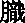
\includegraphics[width=1em]{img/zhi}}”(\lypy{zhí})之误,败臭。次:指肆,市中店铺。)英文\lyurl{http://heptagrama.com/quotes-thoughts-62.htm}{谚语}的建议更直白:\lyqe{Surround yourself with people who make you a better person.}甚至\lyurl{http://www.jimrohn.com/}{Jim John}武断地说:\lyqe{You are the average of the five people you spend the most time with.} 反过来想更容易认同:一直stand out是很累的;环境与时间会磨平棱角。}
}
{}
%TODO:
%择友,择业……Surround yourself with people who make you a better person. (http://www.quora.com/What-are-the-most-important-things-you-should-teach-a-kid)
%
%You are the average of the five people you spend the most time with. --- Jim Rohn. 一直stand out是很累的;时间会磨平棱角。


\lytopics{仁,智,贫富,快乐}
\lyblob{子曰:“不仁者不可以久处约,不可以长处乐。仁者安仁,知者利仁。”}
{
\item \lylabel{yue1}\lyterm{约}:困窘,窘迫,相当于\lylink{qiong2}{穷}。其本义为缠束,既包含物质贫乏的实情,也可指不堪其苦的心境。\lyl{《南史·吉士瞻传》:\lyq{在郡清约,家无私积。}}\lyc{《礼记·坊记》:\lyq{子云:“小人贫斯约,富斯骄;约斯盗,骄斯乱。”}}

\item \lyterm{安仁}:安处于仁。\lyc{《论语集释》按语:\lyq{无所为(\lypy{wèi})而\lylink{wei2b}{为}(\lypy{wéi})之谓之安仁,若有所为而为之,是利之也,故止可谓之智,而不可谓之仁。}(止:通“只”。)\lylabel{renyousan}《礼记·表记》:\lyq{仁有三,与仁同功而异情。与仁同功,其仁未可知也;与仁\lylink{geyuqidang}{同过},然后其仁可知也。仁者安仁,知者利仁,畏罪者强仁。}(同功:效果相同。\lylabel{qiang3}强(\lypy{qiǎng}):勉强,非自发自愿地。)}
}
{}


\lytopics{仁,好恶}
\lyblob{子曰:“唯仁者能好人,能恶人。”}
{
\item \lyterm{能}:指态度适当。这可以从\lylink{ren2}{仁}者爱人、相敬相惜的角度理解。\lyc{\lyref{8.10} \lyq{人而不仁,疾之已甚,乱也。}}
\item \lyterm{好}(\lypy{hào}):喜爱。\lylabel{wu4}\lyterm{恶}(\lypy{wù}):厌恶。
}
{}


\lytopics{志,仁,善恶}
\lyblob{子曰:“苟志于仁矣,无恶也。”}
{
\item \lylabel{gou3a}\lyterm{苟}:表示假设条件的连词,假如,倘若。\lyl{\lyref{13.10} \lyq{苟有用我者,期月而已可也,三年有成。}杜甫《前出塞》:\lyq{苟能制侵\lylink{ling2}{陵},岂在多杀伤?}}
}
{}


\lytopics{仁,道,闻达,好恶,贫富,欲}
\lyblob{子曰:“富与贵,是人之所欲也,不以其道得之,不处也。贫与贱,是人之所恶也,不以其道得之,不去也。君子去仁,恶乎成名?君子无终食之间违仁,造次必于是,颠沛必于是。”}
{
\item \lylabel{fu4}\lyterm{富}:财产多。\lyterm{贵}:地位高。\lylabel{jian4}\lyterm{贱}:地位低下。《论语注疏》:\lyq{乏财曰贫,无位曰贱。}

孔子不崇尚物质享受,但也支持寻求富贵,关键在于坚守道义。\lyc{\lyref{7.12} \lyref{7.16} \lyref{8.13}。《礼记·曲礼上》:\lyq{临财毋\lylink{gou3}{苟}得,临难毋苟免。}}
\item \lylabel{chu3}\lyterm{处}(\lypy{chǔ}):居,停留,安身。\lyterm{去}:离开。
\item 从上下文看,后一个\lyterm{不以其道得之}应指“不以其道免之”。
\item \lyterm{恶乎成名}。\lyterm{恶(\lypy{wū})乎}:怎样,何所。\lylabel{wu1}\lyterm{恶}:疑问副词,相当于何。\lyl{《史记·滑稽列传》:\lyq{先生饮一\lylink{dou3}{斗}而醉,恶能饮一石哉?}}

\lyterm{成名}:最终成就君子之名,实指真正成为君子。这是以\lylink{xiushen}{修身}求仁的标准说的,对应于 \lyref{15.20} \lyq{没世而名不称}、\lyref{16.12} \lyq{民到于今称之}。它与 \lyref{9.2} \lyq{博学而无所成名}的扬名当世,\lyref{13.3} \lyq{必也正名}的以名教下,都不尽相同。

\item \lyterm{终食}:吃完一餐饭(的时间)。
\item \lyterm{造次必于是,颠沛必于是}:仓促忙乱时要这样(指守仁),挫折困顿时也要这样。

\lyterm{造}:仓促。\lyl{《礼记·玉藻》:\lyq{造受命于君前,则书于笏。}(笏(\lypy{hù}):古代大臣朝见君王时所持的手板。)}\lyterm{次}:处,所在。\lyterm{造次}就是忙乱之时,仓促之间,构词上类似来自日文的围棋术语“急所”。后来又引申出片刻、轻率的意思。

\lyterm{颠}:倒,跌倒。\lyl{\lyref{16.1} \lyq{危而不持,颠而不扶。}成语“颠扑不破”(扑:击打)。}\lyterm{沛}:通“跋”,也是跌倒。\lyc{颠沛出自《诗经·大雅·荡》结尾:\lyq{人亦有言:颠沛之揭,枝叶未有害,本实先拨。\lylink{yinjian}{殷鉴}不远,在\lylink{xiachao}{夏后}之世。}(揭:翘起见根。拨:断绝。)是把根基动摇的商朝比作倾倒的大树。}
}  % TODO: 对照孟子“鱼,我所欲也……”?
{}


\lytopics{未见,仁,好恶,学}
\lyblob{子曰:“我未见好仁者,恶不仁者。好仁者,无以尚之;恶不仁者,其为仁矣,不使不仁者加乎其身。有能一日用其力于仁矣乎?我未见力不足者。盖有之矣,我未见也。”}
{
\item \lylabel{weijian}\lyterm{未见}:没见过,强调其少有或难能。这是孔子常用的表达方式,详见\lylink{topicweijian}{主题索引}。
\item \lylabel{shang4}\lyterm{尚}:上,增加,超过。还可用于贬义,凌驾,欺凌。\lyl{《新唐书·杨恭仁传》:\lyq{既贵,不以势尚人,故誉望益重。}}

\item \lylabel{jiahuqishen}\lyterm{加乎其身}:指影响到自己。\lyterm{加}:施加(坏影响),近似于英语的impose (sth on sb)。

\item \lyterm{盖}:副词,表示不十分肯定的推测或判断,大概,也许,应该是。\lyl{\lyref{13.3} \lyq{君子于其所不知,盖阙如也。} \lyref{16.1} \lyq{盖均无贫,和无寡,安无倾。}}\lyc{\lyref{6.12} 孔子对子贡“力不足也”的批评;\lyref{7.30} 对“仁至”的信心,可见儒家的真精神。}
}
{}


\lytopics{过失,仁,友}
\lyblob{子曰:“人之过也,各于其党。观过,斯知仁矣。”}
{
\item \lylabel{dang3a}\lyterm{党}:类,本义为亲族。\lyl{《礼记·坊记》:\lyq{睦于父母之党,可谓孝矣。}}

\lylabel{geyuqidang}\lyterm{各于其党}是说同类人就有相同的局限性,会犯类似的错误。\lyc{\lyref{4.2} \lylink{renyousan}{所引}《礼记·表记》。}
}
{}


\lytopics{学,道,生死}
\lyblob{子曰:“朝闻道,夕死可矣。”}
{
\item \lyterm{朝}(\lypy{zhāo}):早晨。\lyterm{夕}:傍晚,日暮。
}
{}


\lytopics{道,贫富,好恶,志,士}
\lyblob{子曰:“士志于道而耻恶衣恶食者,未足与议也。”}
{
\item \lylabel{shi4c}\lyterm{士}:对成年男子的美称,这是它的基本义。\lyl{《韩诗外传》第8卷第24章:\lyq{士必学问,然后成\lylink{junzi}{君子}。}}有具体所指时,意义较广,《论语》中涉及的有:
\begin{lyitemize}
\item 读书人,知识分子。官职并非士的必要条件,但按儒家传统观念,是应当积极从政的。\lyref{19.13} \lyq{学而优则仕},主语很自然地就是士。向学之士与在位之\lylink{qingdafushi}{士}的区别,类似于双重含义的\lylink{junzi}{君子}。古代不同职业的地位及影响力差别很大,现代的选择面就宽得多了。
\item 引申指理想化的士。这两个意义在《论语》中互有融合,就像现代汉语的男人、英语的man,既可以不带感情色彩地指男性成员,也可以根据上下文环境指真男儿、好汉子。\lyl{\lyref{8.7} \lyq{士不可以不弘毅。}\lyref{14.2} \lyq{士而怀居,不足以为士矣。}1962年Bob Dylan民歌金曲\emph{Blowin' in the Wind}的开头:\lyqe{How many roads must a man walk down, before you call him a man?}}

\item \lylabel{shishi}掌管刑狱的官员,即士师。《论语》中仅有2例:\lyref{18.2} \lyq{柳下惠为士师,三黜。} \lyref{19.19} \lyq{孟氏使阳肤为士师。}
\end{lyitemize}
战国时养士之风盛行,更看重实用的一技之长。此外,士还是最低级别的\lylink{qingdafushi}{贵族阶层},也泛指有官职者。
\item \lyterm{议}:讨论,商量,这里偏重于交流求道的心得体会。\lyc{\lyref{15.40} \lyq{道不同,不相为谋。}1929年,史学家陈寅恪(1890--1969)在王国维纪念碑铭中写道:\lyq{士之读书治学,盖将以脱心志于俗谛之\lylink{zhigu}{桎梏},真理因得以发扬。}(谛:道理。俗谛:即庸俗鄙陋之见。)大概所有走出校园、进入社会的人,都能切身感受“俗谛”的无所不在,更可见专心求道之可贵。}
}
{}


\lytopics{君子,政,义}
\lyblob{子曰:“君子之于天下也,无适也,无莫也,义之与比。”}
{
\item \lyterm{\lylink{shi4b}{适}}:归向,依从。\lyl{成语“无所适从”。}\lylabel{mo4b}\lyterm{莫}:否定词,不,这里指不肯。\lyterm{无适也,无莫也}指没有一定要怎样,也没有一定不要怎样,不存着先入之见,预定之规。成语“无适无莫”指待人处事不分远近厚薄,一碗水端平。\lyl{《三国志·吴书·顾雍传》:\lyq{其所选用文武将吏,各随能所任,心无适莫。}}
% NOTE: 莫解作不肯,同《四书集注》。
\item \lyterm{义之与比}:“\lylink{ozhiv}{O之V}”的倒装结构,以符合\lylink{yi4}{义}为标准。\lyterm{比}:并排,并列,引申为拟照,依据。\lyc{《尸子·仁意》有一句话,可作本章的注脚:\lyq{内举不避亲,外举不避仇。仁者之于善也,无择也,无恶也,惟善之所在。}}
}
{}


\lytopics{君子,小人,好恶,德,利}
\lyblob{子曰:“君子怀德,小人怀土;君子怀刑,小人怀惠。”}
{
\item \lyterm{君子}、\lyterm{小人}分别指居上位者和平民百姓,也就是治人者和治于人者。本章反映了孔子的政治模型。\lyc{\lyref{12.19} 君子之德与小人之德。《孟子·滕文公上》:\lyq{无君子莫治\lylink{yeren}{野人},无野人莫养君子。}}
\item \lyterm{怀}:心中存想,关心,在意,care about。\lyterm{怀土}:安心满足于眼前的存身之地,后来引申为思念故乡。\lyl{《汉书·叙传》:\lyq{寤戍卒之言,断怀土之情。}(\lylink{wumei}{寤}:引申为醒悟。)}
\item \lyterm{刑}:法度,规范。\lyl{《左传·襄公二十七年》:\lyq{君失其信,而国无刑,不亦难乎!}}
\item \lylabel{hui4}\lyterm{惠}:恩惠,利益。\lyl{\lyref{17.6} \lyq{惠则足以使人。}}\lyc{《谷梁传·隐公元年》:\lyq{《\lylink{chunqiu}{春秋}》贵义不而不贵惠,信道而不信邪。}}
}
{}


\lytopics{利,行,怨}
\lyblob{子曰:“放于利而行,多怨。”}
{
\item \lyterm{放}(\lypy{fǎng}):依据,依照。\lyterm{放于利而行}指怎么获利多就怎么干,唯利是图。
\item \lylabel{yuan4a}\lyterm{怨}:仇恨,怨恨,这是其本义。\lyl{\lyref{14.34} \lyq{以德报怨,何如?}}
}
{}


\lytopics{礼,政}
\lyblob{子曰:“能以礼让为国乎,何有?不能以礼让为国,如礼何?”}
{
\item \lylabel{wei2b}\lyterm{为}(\lypy{wéi}):动词,等于一般性的做,do,可以搭配的对象很宽泛,要根据上下文具体理解。\lyterm{为国}:指治国理政。\lyc{《韩诗外传》第1卷第5章:\lyq{人之命在天,国之命在礼。君人者,降礼尊贤而\lylink{wangdao}{王},重法爱民而霸,好利多诈而危,权谋倾覆而亡。}《左传·襄公十三年》:\lyq{让,礼之主也。\lycharlink{fanxuanzi}{范宣子}让,其下皆让。……世之治也,君子尚能而让其下,小人农力以事其上,是以上下有礼,而谗\lylink{te2}{慝}\lylink{chu4}{黜}远,由不争也,谓之懿德。及其乱也,君子称其功以\lylink{jia1a}{加}小人,小人\lylink{fa2}{伐}其技以\lylink{ping2}{冯}君子,是以上下无礼,乱虐并生,由争善也,谓之昏德。国家之敝,恒必由之。}(农力:努力。)《战国策》刘向书录:\lyq{五\lylink{zhuhou}{伯}之起,尊事周室。五伯之后,……犹以义相支持,歌说以相感,聘觐以相交,期会以相一,盟誓以相救。天子之命,犹有所行;会享之国,犹有所耻;小国得有所依,百姓得有所息。故孔子曰:“能以礼让为国乎,何有?”周之流化,岂不大哉!}}
\item \lylabel{heyou}\lyterm{何有}:字面上是说有什么呢,多用于反问,可表达的意思包括:有什么难的呢,有什么关系呢,有什么值得看重的呢,有什么好在乎的呢,这里是第一个意思。\lyl{\lyref{6.8} \lyq{于从政乎何有?}《史记·齐太公世家》颜师古注:\lyq{人之情非不爱其身也,其身之忍,又将何有于君?}《左传·僖公二十四年》:\lyq{除君之恶,唯力是视,蒲人狄人,余何有焉?}李贽《与周友山》:\lyq{士为知己者死,死且甘焉,又何有于废弃\lylink{yu2}{欤}?}}
}
{}


\lytopics{忧患,仕隐,人我,才能,知,学}
\lyblob{子曰:“不患无位,患所以立。不患莫己知,求为可知也。”}
{
\item \lyterm{患所以立}:担心(自己没有)赖以\lylink{erli}{立身}的东西。孔子指的是才德,也可以理解成广义上的能力、资本。
\item \lyterm{莫己\lylink{zhi1b}{知}}:“\lylink{nov}{NOV}”的倒装结构。\lyterm{莫}是否定代词,没有人。
\item \lyterm{求为可知}:寻求值得被别人重视、称道的东西。
}
{}


\lytopics{道,忠,恕}
\lybloba{子曰:“\lychar{参}乎!吾道一以贯之。”\lychar{曾子}曰:“唯。”

子出,门人问曰:“何谓也?”曾子曰:“夫子之道,忠恕而已矣。”}
{
\begin{lyblobitemize}
\item \lylabel{yiyiguanzhi}\lyterm{一以贯之}:“以一贯之”的倒装,一个基本道理贯通它的全部内容。古注常用钱绳串铜钱来打比方,用现代的话说,就是既有体系规模,又有中心思想。
\item \lyterm{唯}:表示同意的答应声,相当于是的,yes。参见\lylink{nuo4}{诺}。\lyl{成语“唯唯诺诺”指人一味应声附和,而不发表自己的意见。}
\item \lylabel{menren}\lyterm{门人}:弟子,学生。古代以登师\lyterm{门}求学为礼。\lyc{《礼记·曲礼上》:\lyq{礼闻来学,不闻往教。}孔颖达疏:\lyq{凡学之法,当就其师,处\lylink{nanmian}{北面}伏\lylink{ying1}{膺}。……不可以屈师亲来就己。}《仪礼·士相见礼》唐代贾公彦疏:\lyq{学生事师,虽无\lylink{wufu}{服},有父兄之恩,故称弟子也。}}
% NOTE: 据《辞源》转引清代阎若璩《四书释地三续》,古代弟子、门人无区别,至后汉时公卿自多教授聚徒,亲受业者为弟子,转相传授者为门人。

《论语》中没有直接标明的门人,都是指孔子的弟子。\lyref{8.3} 的“门弟子”指曾子的弟子。
\item \lylabel{shu4}\lyterm{恕}:推己及人。从字形结构看,可以理解为视人心如己心。更精准的解释是 \lyref{15.24} \lyq{己所不欲,勿施于人。}《说文解字》直接解释为仁,也就是“恕”的正向表现:\lyref{6.30} \lyq{己欲立而立人,己欲达而达人。}\lyc{《尸子·恕》:\lyq{恶\lylink{zhu1}{诸}人,则去诸己;欲诸人,则求诸己——此恕也。}}
\end{lyblobitemize}
\lylink{ren2}{仁}是儒家的至高追求。实践上,\lylink{zhong1}{忠}指做事(包括\lylink{3.19}{事君}),恕指做人。根据曾子的解读,忠+恕=臻于仁的最佳途径。\lyc{据《宋史·范纯仁传》,范仲淹之子、北宋名臣范纯仁\lyq{性\lylink{yi2}{夷}易宽简,不以声色加人,谊之所在,则挺然不少屈。……尝曰:“吾平生所学,得之‘忠恕’二字,一生用不尽,以至立朝事君,接待僚友,亲睦宗族,未尝须臾离此也。”每戒子弟曰:“人虽至愚,\lylink{ze2a}{责}人则明;虽有聪明,恕己则昏。\lylink{gou3a}{苟}能以责人之心责己,恕己之心恕人,不患不至圣贤地位也。”}(\lylabel{xuyu}须臾(\lypy{yú}):片刻。\lylabel{yi4j}谊:通“\lylink{yi4}{义}”。)}
}
{
} % TODO: 如果用在个人修养方面,“忠”也可以理解成忠于自己的内心,努力认识自己、把握自己。“恕”可以认为是宽容之心,理解并欣然接受别人是与自己不同、但又完全合理的个体,不苛求,不狭隘。


\lytopics{君子,小人,义,利}
\lyblob{子曰:“君子喻于义,小人喻于利。”}
{
\item \lyterm{喻}:明白(道理),了解(情况)。\lyl{成语“不言而喻”、“家喻户晓”。}

其本义为告知、开导(人),前面相当于它的被动用法。\lylabel{xiao3}“晓”也有这两种意思。\lyl{成语“不可理喻”、“晓以利害”。}

这句话不是说君子并不求利,而是先后轻重的次序与小人相反。\lyc{\lyref{4.5}}
}
{}


\lytopics{学,反省}
\lyblob{子曰:“见贤思齐焉,见不贤而内自省也。”}
{
\item \lyterm{思齐}:想要(与贤)看齐。
}
{}


\lytopics{孝,敬}
\lyblob{子曰:“事父母几谏,见志不从,又敬不违,劳而不怨。”}
{
\item \lyterm{几(\lypy{jī})\lylink{jian4c}{谏}}:含蓄轻微地劝谏,与直谏、力谏、\lylink{qie4b}{切}谏相反。\lylabel{ji1b}\lyterm{几}:隐微。\lyl{成语“审几度势”(引申为苗头,迹象)。}\lyc{《礼记·祭义》:\lyq{孝子如执玉,如奉盈,洞洞属属然如弗胜,如将失之。严威\lylink{yan3}{俨}恪,非所以事亲也,成人之道也。}(洞洞、属属(\lypy{zhǔ}):都是专心谨敬的样子。恪(\lypy{kè}):恭敬。)《孟子·万章上》:\lyq{父母爱之,喜而不忘;父母恶之,劳而不怨。}(之:指子女。)《礼记·坊记》说,子女成年就应多尽孝心,而不该要求父母还像童年时那样慈爱待己:\lyq{言\lylink{xiao4}{孝}不言\lylink{ci2}{慈}……民犹薄于孝而厚于慈。}}
}
{}


\lytopics{孝}
\lyblob{子曰:“父母在,不远游,游必有方。”}
{
\item \lyterm{游}:出行,离家在外。
\item \lyterm{有方}:有明确的方位处所,指告诉父母自己要去哪儿,免得父母担心。\lyc{《礼记·曲礼上》:\lyq{夫为人子者,出必告,反必面,所游必有常,所习必有业,恒言不称老。}(面:相见,特指下往见上,拜见。\lylink{heng2a}{恒}言不称老:平常说话不自称老。)}
}
{}


\lytopics{孝}
\lybloba{子曰:“三年无改于父之道,可谓孝矣。”}
{
见 \lyref{1.11}。
}
{}


\lytopics{孝}
\lyblob{子曰:“父母之年,不可不知也,一则以喜,一则以惧。”}
{
\item \lyterm{年}:年龄。\lyc{《孔子家语·致思》:\lyq{夫树欲静而风不停,子欲养而亲不待。往而不来者,年也;不可再见者,\lylink{qinqin}{亲}也。}亦见子路\lylink{weiqinfumi}{为亲负米}。}
}
{}


\lytopics{言,行,耻}
\lyblob{子曰:“古者言之不出,耻躬之不逮也。”}
{
\item \lylabel{gong1a}\lyterm{躬}:本义为身体,引申为自己,自身。\lyl{成语“事必躬亲”。}
\item \lylabel{dai4c}\lyterm{逮}(\lypy{dài}):本义为追及,catch up,引申为达到,及。\lyl{成语“力有未逮”。}
}
{}


\lytopics{过失}
\lyblob{子曰:“以约失之者鲜矣。”}
{
\item \lyterm{约}:节制,约束,不放纵。\lyl{\lyref{6.27} \lyq{君子博学于文,约之以礼。}}

\item \lylabel{shizhizhe}\lyterm{失之者}:犯错的。\lyterm{失}:犯错误,有过失。代词\lyterm{之}的所指趋于虚化,突出了动作“失”,也舒缓了语气。从英文语法的角度理解,及物动词与“之”连用,就变成不及物动词。\lyl{\lyref{6.20} \lyq{知之者不如好之者,好之者不如乐之者。}《左传·庄公十年》:\lyq{公将鼓之,刿曰:“未可。”}}
}
{}


\lytopics{君子,言,行}
\lyblob{子曰:“君子欲讷于言而敏于行。”}
{
\item \lylabel{ne4}\lyterm{讷}(\lypy{nè}):本义为口齿笨拙,引申为少言寡语。成语“讷言敏行”指出言谨慎,做事麻利。\lyc{\lyref{1.14} \lyq{君子……敏于事而慎于言。}据《大戴礼记·曾子疾病》,\lycharlink{zengshen}{曾参}临终前感慨:\lyq{华繁而实寡者,天也;言多而行寡者,人也。}(华:通“花”。)}
}
{}


\lytopics{德,友}
\lyblob{子曰:“德不孤,必有邻。”}
{
\item \lyterm{邻}:指亲近的人,志趣相投的朋友。
}
{}


\lytopics{君臣,友}
\lyblob{\lychar{子游}曰:“事君数,斯辱矣;朋友数,斯疏矣。”}
{
\item \lyterm{数}(\lypy{shuò}):多次,屡次,这里指过于殷勤琐碎,让人烦不胜烦。\lyc{比较 \lyref{3.18},体会与人交往的分寸。}
\item \lyterm{疏}:不亲近,疏远。
}
{}



\chapter{公冶长}
%%%%%%%%%%%%%%%%%%%%%%%%%%%%%%%%%%%%%%%%%%%%%%%%%%%%%%%%%%%%

\lytopics{过失}
\lyblob{子谓\lychar{公冶长}:“可妻也。虽在缧绁之中,非其罪也。”以其子妻之。}
{
\item \lyterm{妻}(\lypy{qì}):动词,(把女子)嫁(给某人为妻)。另外也可以表示娶(女子为妻)。\lyl{《史记·五帝本纪》:\lyq{\lycharlink{yao}{尧}妻\lycharlink{shun}{之}二女,观其德于二女。}《孟子·万章上》写\lycharlink{shun}{舜}因为难讨父母欢心而苦恼:\lyq{好色,人之所欲,妻帝之二女,而不足以解忧。}}
\item \lylabel{leixie}\lyterm{缧绁}(\lypy{léi xiè}):囚禁,监狱。分开来看,\lyterm{缧}是绑犯人的黑绳,\lyterm{绁}是牵狗、马等牲畜的绳索。\lylabel{zhigu}构词类似的又如桎梏(\lypy{zhì gù}),本义是木制的脚镣和手铐,引申为拘禁,束缚。
\item \lyterm{以其子妻之}:(孔子)把自己的女儿嫁给了公冶长。\lylabel{zi3a}\lyterm{子}:古代兼指儿子或女儿。这就像\lylink{gongzi}{公子}可以兼指诸侯的子女。\lyl{韩愈《试大理评事王君墓志铭》:\lyq{生三子,一男二女。}}
}
{}


\lytopics{仕隐}
\lyblob{子谓\lychar{南容}:“邦有道,不废;邦无道,免于刑戮。”以其兄之子妻之。}
{
\item \lylabel{fei4}\lyterm{废}:弃置不用,搁置。\lyterm{不废}指人尽其才而用,这里实指愿意承担社会责任,入世从政。
\item \lyterm{其兄}:指孔子的哥哥孟皮。孟皮由于腿脚有残疾,不适合继承家族身份(\lylink{qingdafushi}{士}),所以由孔子继承,有了话语权。% TODO: 写入源流,并加链接。
}
{}  % TODO: 与世推移,对自己的侄女负责?


\lytopics{君子,学}
\lyblob{子谓\lychar{子贱}:“君子哉若人!鲁无君子者,斯焉取斯?”}
{
\item \lyterm{若}:近指代词,这,此。\lyl{《孟子·梁惠王上》:\lyq{以若所为,求若所欲,犹缘木而求鱼也。}(缘:攀爬。)}孔子也用这句话\lylink{14.5}{称赞过}南宫适。

\item \lylabel{zhe3}\lyterm{者}:表示假设的助词,用于复合句中前一分句的末尾:假如鲁国没有(其他)君子的话……放在这个位置的\lyterm{者}还可表示判断。\lyl{\lyref{6.28} \lyq{予所否者,天厌之!天厌之!} \lyref{6.30} \lyq{夫仁者,己欲立而立人,己欲达而达人。}}
\item \lyterm{斯焉取斯?}:他是从哪里学到这种品德的呢?第一个\lyterm{斯}指子贱,第二个指作为君子的品德。\lyterm{取}:指效法,吸取。

《说苑·政理》记载了孔子这句赞叹的来历。孔子有个侄子与子贱同期为官,孔子问侄子从仕以来的所得所失,回答是无所得而有三失:政务繁忙荒废了学业,薪水微薄疏远了亲戚,公事多急怠慢了朋友。又问子贱,回答却是无所失而有三得:\lyq{始诵之文,今履而行之,是学日益明也,所得者一也;奉禄虽少,鬻鬻得及亲戚,是以亲戚益亲也,所得者二也;公事虽急,夜勤吊死视病,是以朋友益亲也,所得者三也。}(鬻(\lypy{zhōu}):通“粥”。)
}
{}


\lytopics{才能}
\lyblob{\lychar{子贡}问曰:“\lychar{赐}也何如?”子曰:“女器也。”

曰:“何器也?”曰:“瑚琏也。”}
{
\item \lyterm{瑚}和\lyterm{琏}(\lypy{liǎn})都是古代\lylink{zongmiao}{宗庙}中盛\lylink{wugu}{五谷}的礼器。\lyterm{瑚琏}比喻善于治国理政、庙堂之上的\lylink{qi4}{人才}。
}
{}


\lytopics{仁,言,好恶}
\lyblob{或曰:“\lychar{雍}也仁而不佞。”

子曰:“焉用佞?御人以口给,屡憎于人。不知其仁,焉用佞?”}
{
\item \lylabel{ning4}\lyterm{佞}(\lypy{nìng}):有口才,能言善辩。后来“不佞”用于谦称自己,“佞人”偏指善于花言巧语、阿谀奉承的人。\lyc{东汉王充《论衡·答佞》:\lyq{诸非皆恶。恶中之逆者,谓之无道;恶中之\lylink{qiao3}{巧}者,谓之佞人。}}
\item \lyterm{\lylink{yu4b}{御}}:约束以为己用,即统治,管理。\lyl{成语“以简御繁”。}
\item \lyterm{口给}(\lypy{jǐ}):口齿伶俐,能说会道。\lyterm{给}:充足。\lyl{成语“家给人足”。}
\item \lyterm{不知其仁,焉用佞?}:不知道他算不算仁,可为什么要有口才(才算好)呢?\lylink{4.24}{行重于言}是孔子的一贯主张。

\lyterm{不知}在这里表示让步,有“且不说”的意味。这也是孔子委婉表示否定的常用句式,可以比较 \lyref{4.6} 的\lylink{weijian}{未见}。\lyl{\lyref{5.8} \lyref{5.19} \lyref{14.1}}
}
{}


\lytopics{仕隐}
\lyblob{子使\lychar{漆雕开}仕,对曰:“吾斯之未能信。”子说。}
{
\item \lylabel{shi4a}\lyterm{仕}:做官,从政。也可作名词,官职。\lyl{《北史·徐招传》:\lyq{初入洛阳,虽未登仕,已为时知。}“仕途”即官位升迁之路。}

\item \lyterm{吾斯之未能信}:“\lylink{ozhiv}{O之V}”的倒装结构。\lyterm{斯}指仕,\lyterm{信}指有自信。
}
{}


\lytopics{仕隐,勇}
\lyblob{子曰:“道不行,乘桴浮于海,从我者其\lychar{由}与?”\lychar{子路}闻之喜。子曰:“由也好勇过我,无所取材。”}
{
\item \lyterm{桴}(\lypy{fú}):小木筏,小竹筏。\lyterm{道不行}是假设。\lyterm{浮于海}指遁世隐居,参见 \lyref{18.9}。
\item \lyterm{无所取材}:这是批评子路除了勇很突出之外,就没什么可取的优点了。\lyc{\lyref{17.23}}

\lyterm{材}一语双关,也可以指做桴之材,语含打趣。在刚开始得意时泼点冷水,是孔子对老学生的爱护,子路的忠勇热诚,也宽慰了孔子的心情。
}
{}


\lytopics{仁,政,用人}
\lyblob{\lychar{孟武伯}问:“\lychar{子路}仁乎?”子曰:“不知也。”又问,子曰:“\lychar{由}也,千乘之国,可使治其赋也,不知其仁也。”

“\lychar{求}也何如?”子曰:“求也,千室之邑,百乘之家,可使为之宰也,不知其仁也。”

“\lychar{赤}也何如?”子曰:“赤也,束带立于朝,可使与宾客言也,不知其仁也。”}
{
\item \lyterm{治其赋}:领导、训练其军队。\lyterm{赋}:田地税,因为当时是根据田地面积计算人口去服\lylink{bingyi}{兵役},所以引申指军队。

\item \lylabel{yi4c}\lyterm{邑}(\lypy{yì}):城镇,大小不等,常作为天子赐予诸侯,或诸侯赐予卿大夫的封地。一邑之宰多由家臣担任。\lyc{《左传·庄公二十八年》:\lyq{凡邑,有宗庙先君之主曰都,无曰邑。邑曰筑,都曰城。}(主:即神主,祭祀用的牌位。)}

\lyterm{千室之邑}与\lyterm{百\lylink{sheng4a}{乘}之\lylink{jia1}{家}}所指相同,均为卿大夫的封邑。\lyq{室}:家庭,住户。\lyc{据皇侃义疏,\lyq{地方一里为井,井有三家}(家即室),则1000室之邑约合地方18.3里。按《左传·成公元年》杜预注,64井出兵车1乘,直接推算的话,100乘之家合地方80里,比于诸侯了。但“千室”可以换算为领地,“百乘”则是礼制。天子地方千里,合15625乘,符合\lylink{bingyi}{万乘之尊}的定位。}

\item \lyterm{宰}:即家宰,卿大夫家里的总管,管家。
}
{}


\lytopics{学,智}
\lyblob{子谓\lychar{子贡}曰:“女与\lychar{回}也孰愈?”对曰:“\lychar{赐}也何敢望回?回也闻一以知十,赐也闻一以知二。”子曰:“弗如也,吾与女,弗如也!”}
{
\item \lyterm{愈}:胜,优。\lyl{\lyref{11.16} \lyq{然则师愈与?}}

\item \lyterm{与女}:赞同你。\lylabel{yu3a}\lyterm{与}:动词,同意,赞许。\lyl{\lyref{11.26} \lyq{夫子喟然叹曰:“吾与点也!”}}
}
{}


\lytopics{学,孔子自评,言,行,识人}
\lyblob{\lychar{宰予}昼寝。子曰:“朽木不可雕也,粪土之墙不可杇也。于\lychar{予}与何诛?”

子曰:“始吾于人也,听其言而信其行;今吾于人也,听其言而观其行。于予与改是。”}
{
\item \lyterm{昼寝}:白天睡大觉。
\item \lyterm{粪土之墙}:用污泥脏土砌成的墙,质地混杂,表面很不平整,这在今天的农村仍能见到。连用这两个比喻,可见孔子的伤心失望。
\item \lyterm{杇}(\lypy{wū}):粉刷墙壁用的泥抹子,这里作动词,粉饰,涂饰。
\item \lyterm{于予与(\lypy{yú})何诛}。\lylabel{yu2a}\lyterm{与}:助词,用于句中表示停顿。\lyterm{诛}:谴责,斥责,这是其本义,后来才引申为讨伐,杀戮。\lyl{成语“口诛笔伐”。}
}
{}  % TODO: 孔子显然认为:首先要态度端正,才有可能出成绩。是否合理合适?


\lytopics{未见,欲,刚}
\lyblob{子曰:“吾未见刚者。”或对曰:“\lychar{申枨}。”子曰:“枨也欲,焉得刚?”}
{
\item \lylabel{gang1}\lyterm{刚}:本义为坚硬,引申为坚强,不动摇。其甲骨文字形为以利刃斩断罗网。
\item \lylabel{yu4d}\lyterm{欲}:贪欲,欲求,这里指欲求多。\lyc{林则徐1839年所作对联:\lyq{海纳百川,有容乃大;壁立千\lylink{ren4}{仞},无欲则刚。}}
}
{}  % TODO: 佛教的“刚”?埃德加·爱伦·坡(Edgar Allan Poe)1838年的小说《丽姬娅》(\emph{Ligeia})反复出现的话:\lyq{凡人若无意志薄弱之缺陷,决不臣服天使,亦不屈从死神。}(Man doth not yield himself to the angels, nor unto death utterly, save only through the weakness of his feeble will.)



\lytopics{人我,欲}
\lyblob{\lychar{子贡}曰:“我不欲人之加诸我也,吾亦欲无加诸人。”子曰:“\lychar{赐}也,非尔所及也。”}
{
\item \lylabel{jia1a}\lyterm{加}:欺凌,侵犯。这是从\lylink{jiahuqishen}{施加(坏影响)}的意思引申来的。\lyc{\lyref{15.24}} % NOTE: 亦参《韩诗外传》第9卷第7章。
}
{}


\lytopics{人评孔子}
\lybloba{\lychar{子贡}曰:“夫子之文章,可得而闻也。夫子之言性与天道,不可得而闻也。”}
{
\begin{lyblobitemize}
\item \lylabel{wenzhang}\lyterm{文章}:指道德礼仪,人文教化。\lyl{\lyref{8.19} \lyq{焕乎,其有文章。}}\lyc{《四书集注》:\lyq{文章,德之见于外者,威仪文辞皆是也。}}
\item \lyterm{性}:人的本性。孔子很少谈论这种抽象哲学问题,《论语》中唯一说到性的地方,是 \lyref{17.2} \lyq{性相近也,习相远也。} % NOTE: \lyref{17.3} \lyq{唯上知与下愚不移}也接近。
\item \lyterm{天道}:天之道,即世间万物发展变化的抽象规律。孔子教人求仁,注重力行,不尚玄虚,但并不等于孔子对天道缺乏兴趣。如果用“学究天人”形容孔子,对《\lylink{yijing}{易经}》的研究就体现了“天”的部分。\lyc{《周易·说卦》:\lyq{昔者圣人之作《易》也,将以顺性命之理。是以立天之道曰阴与阳,立地之道曰柔与刚,立人之道曰仁与义。}\lylink{zhouchao}{春秋}时起,人的主观能动性逐渐得到重视,不再单纯信奉天意神力了。《逸周书·文传》:\lyq{兵强胜人,人强胜天。能制\lylink{qi2}{其}有者,则能制人之有;不能制其有者,则人制之。}(制:控制,掌握。)《孟子·尽心上》提出天道自在人心:\lyq{尽其心者,知其性也。知其性,则知天矣。存其心,养其性,所以事天也。夭寿不贰,修身以\lylink{si4a}{俟}之,所以立命也。}(夭寿不贰:无论短命还是长寿都不变心。)《荀子·天论》的天道则更接近自然规律:\lyq{天行有常,不为\lycharlink{yao}{尧}存,不为\lycharlink{xiachao}{桀}亡。应之以治则吉,应之以乱则凶。……唯圣人为不求知天。……故君子敬其在己者,而不慕其在天者;小人\lylink{cuo4}{错}其在己者,而慕其在天者。}}
% NOTE: 《左传·昭公十八年》:\lyq{\lycharlink{zichan}{子产}曰:“天道远,人道\lylink{er3}{迩}。非所及也,何以知之?”}
\end{lyblobitemize}
\lyc{因为子贡这段话,后世认为“性与天道”就是圣人之学的高阶课程,并产生这样的错觉:如果先学、多谈它们就能一步到位,岂不便捷闪耀?这种跃进的想象,\lylink{helouzhiyou}{侥幸}的心理,逐渐滋生了轻视基础建设、迷信上层架构的投机浮夸风气。1667年,顾炎武在《与友人论学书》中说:\lyq{性也,命也,天也,夫子之所罕言,而今之君子之所\lylink{heng2a}{恒}言也;出处、\lylink{qujiu}{去就}、辞受、取与之辨,孔子孟子之所恒言,而今之君子所罕言也。谓\lylink{5.19}{忠与清}之未至于仁,而不知不忠与清而可以言仁者,未之有也;谓\lylink{9.27}{不忮不求}不足以尽道,而不知终身于忮且求而可以言道者,未之有也。}(出处(\lypy{chǔ}):出仕与隐退。)他在《日知录·卷七·夫子之言性与天道》中,再次痛陈了空谈弄玄之弊:\lyq{昔之清谈,谈老庄;今之清谈,谈孔孟。未得其精,而已遗其粗,未究其\lylink{ben3}{本},而先辞其\lylink{mo4c}{末}。不习\lylink{liuyi}{六艺}之文,不考百王之典,不综当代之务,举夫子论学、论政之大端一切不问,而曰\lylink{yiyiguanzhi}{一贯}、曰\lylink{17.19}{无言}。以明心见性之空言,代修己治人之实学,\lylink{gugong}{股肱}惰而万事荒,爪牙亡而\lylink{siguo}{四国}乱,神州荡覆,宗社丘墟。}(百王:历代帝王。综:治理。爪牙:比喻武将。)}
}
{}  % TODO: 弟子的资质?


\lytopics{学,行}
\lybloba{\lychar{子路}有闻,未之能行,唯恐有闻。}
{
\begin{lyblobitemize}
\item \lyterm{有闻}:指新学了一个道理。后面的\lyterm{唯恐有闻}指“唯恐又有闻”。这是写子路学有所得之后的力行之速。\lyc{《\lylink{dizigui}{弟子规}》:\lyq{方读此,勿慕彼。此未终,彼勿起。}}
\end{lyblobitemize}
\lyc{《荀子·儒效》论述了学习过程中知与行的递进关系:\lyq{不闻不若闻之,闻之不若见之,见之不若知之,知之不若行之。学至于行之而止矣。}这里的“闻”显然比子路的程度浅,只是听说有这么回事,是学的萌芽。西方常以为这句话是孔子说的:\lyqe{I hear and I forget. I see and I remember. I do and I understand.}}
% NOTE: http://english.stackexchange.com/questions/226886/origin-of-i-hear-and-i-forget-i-see-and-i-remember-i-do-and-i-understand
}
{}


\lytopics{学,耻}
\lyblob{\lychar{子贡}问曰:“\lychar{孔文子}何以谓之‘文’也?”

子曰:“敏而好学,不耻下问,是以谓之‘文’也。”}
{
\item \lylabel{min3a}\lyterm{\lylink{min3}{敏}}:头脑反应快,聪慧。\lyl{\lyref{12.1} \lyq{回虽不敏,请事斯语矣。}成语“敬谢不敏”是以自己能力不够来婉言推辞。}
\item \lyterm{文}:孔文子的谥号。据《逸周书·谥法解》,可以称“文”的有27种品德,这里相符的是“勤学好问曰文”。
\item \lyterm{不耻下问}:愿意向比自己地位低、水平差的人询问请教,而不觉得没面子。思考:“要面子”和“不要脸”是怎样形成并且共存的?为什么“耻”会选择性地消失?
}
{}


\lytopics{君子,人我,君臣,人民,恭,敬,惠,义}
\lyblob{子谓\lychar{子产}:“有君子之道四焉:其行己也恭,其事上也敬,其养民也惠,其使民也义。”}
{
\item \lylabel{xingji}\lyterm{行己}:自己立身做事,behave oneself。\lyl{\lyref{13.20} \lyq{行己有耻。}}
\item \lylabel{hui4a}\lyterm{惠}:宽厚仁爱。\lyc{\lyref{14.9} \lyq{或问子产,子曰:“惠人也。”}}
\item \lyterm{义}:宜,适合,指顺应民心,不扰民。\lyref{6.22} \lyq{务民之义}里也是这个意思。
}
{}


\lytopics{才能}
\lyblob{子曰:“\lychar{晏平仲}善与人交,久而敬之。”}
{
\item \lyterm{之}指“晏平仲”或“人”都讲得通,可以自行理解,不必拘泥于一说。
}
{}


\lytopics{俭奢,智}
\lyblob{子曰:“\lychar{臧文仲}居蔡,山节藻棁,何如其知也?”}
{
\item \lyterm{居蔡}:盖房子供养大乌龟。\lylabel{caigui}\lyterm{蔡}:占卜用的大乌龟,古人相信越大的龟壳占卜起来越灵验。
\item \lyterm{山节藻棁}(\lypy{zhuō})是天子专用的庙饰,臧文仲用于龟房,可见排场之隆重。\lyterm{山节}:雕成山形的柱头斗拱。\lyterm{藻棁}:画有藻纹的梁上短柱。
\item \lyterm{何如其\lylink{zhi4d}{知}也?}:他哪里聪明呢?\lylabel{siyuanju}\lyc{臧文仲确实有迷信灵物的倾向。《国语·鲁语上》载,有一种叫爰(\lypy{yuán})居的巨型海鸟盘桓在鲁国东门外三天不飞走,臧文仲就让\lylink{guoren}{国人}向它祭祷。这种滥用祀典的行为受到\lycharlink{liuxiahui}{柳下惠}有理有据的批评:\lyq{“越哉,臧孙之为政也!夫祀,国之\lylink{dajie}{大节}也,而节,政之所成也。故慎制祀以为国典。……今海鸟至,己不知而祀之,以为国典,难以为仁且智矣。……今\lylink{zi1}{兹}海其有灾乎?夫广川之鸟兽,恒知避其灾也。”}(国典:国家的典章制度。)臧文仲听到后承认:\lyq{“\lylink{xin4a}{信}吾过也!季子之言,不可不法也。”使书以为三策。}(策:书简。)}
}
{}


\lytopics{仕隐,色,仁,忠,清}
\lyblob{\lychar{子张}问曰:“令尹子文三仕为令尹,无喜色,三已之,无愠色,旧令尹之政必以告新令尹。何如?”子曰:“忠矣。”曰:“仁矣乎?”曰:“未知,焉得仁?”

“崔子弑齐君,陈文子有马十乘,弃而违之。至于他邦,则曰:‘犹吾大夫崔子也。’违之。之一邦,则又曰:‘犹吾大夫崔子也。’违之。何如?”子曰:“清矣。”曰:“仁矣乎?”曰:“未知,焉得仁?”}
{
\item \lylabel{lingyin}\lyterm{令尹}:春秋战国时期楚国的最高官职,内理政务(相当于宰相),外掌兵权,多由王室亲族担任。

\item \lyterm{子文}:斗谷於菟(\lypy{wū tú}),字子文,前664年--前637年间任楚国令尹,清廉爱民,上任后献出家产解救国难,留下了“毁家纾难”的佳话。(纾(\lypy{shū}):缓和,解除。)他荐举的继任令尹子玉,就是晋楚\lylink{chengpuzhizhan}{城濮之战}的楚军统帅。
% NOTE: 斗谷於菟是楚国令尹斗伯比的私生子,被遗弃于郊野后,有母老虎给他喂奶。当时楚语称乳为“谷”,老虎为“於菟”,于是给他起了“谷於菟”之名。

\item \lylabel{yi3b}\lyterm{已}:停止,引申为罢免,离职。\lyterm{三仕}、\lyterm{三已}的详情难以确考。\lyc{《国语·楚语下》载,\lyq{昔斗子文三舍令尹,无一日之积,\lylink{xu4c}{恤}民之故也。}楚成王听说他家吃了上顿没下顿,每次想给他加薪,他都逃不从命。\lyq{人谓子文曰:“人生求富,而子逃之,何也?”对曰:“夫从政者,以庇民也。民多旷者,而我取富焉,是勤民以自\lylink{feng1}{封}也,死无日矣!我逃死也,非逃富也。”}(旷:空乏,穷匮。勤:劳。)《史记·循吏列传》对于楚国名相孙叔敖也有类似的评价:\lyq{三得相而不喜,知其材自得之也;三去相而不侮,知非己之罪也。}}

\item \lyterm{弑}(\lypy{shì}):臣杀君,子杀父。\lylabel{cuizhu}\lyterm{崔子弑齐君}:指前548年齐国大夫崔杼(\lypy{zhù})纵容家臣弑杀国君齐庄公一事。庄公名光,齐国第22任国君,前554年由崔杼迎立,后来却屡与崔杼之妻通奸。崔杼怀恨在心,告病不朝,庄公借口探病,上门逐戏崔杼妻。崔杼的家臣堵住庄公,崔杼闭内门不纳,庄公被杀。崔杼虽未亲手杀死庄公,却心怀不轨在前,纵凶不救在后,所以齐国太史仍秉笔直书“崔杼弑庄公”。孔子时年4岁。事见《左传·襄公二十五年》、《史记·齐太公世家》。
\item \lylabel{chenwenzi}\lyterm{陈文子}:齐庄公的大夫,名须无,也称田文子。他是田氏家族的第4代宗主,\lycharlink{chenchengzi}{陈成子}的曾祖父。
\item \lyterm{违}:离开,这是其本义。\lyl{《吴子·图国》:\lyq{谋者,所以违害就利。}}
\item \lyterm{犹吾大夫崔子也}:指该国的主政大臣也像崔杼一样残暴无礼。
\item \lyterm{清}:洁净,清白,其本义为水纯净透明,不含杂质。
}
{}


\lytopics{行,谨慎}
\lyblob{季文子三思而后行。子闻之,曰:“再,斯可矣。”}
{
\item \lylabel{jiwenzi}\lyterm{季文子}(?--前568年):季孙行父,\lycharlink{jiyou}{季友}之孙,\lycharlink{jishi}{季孙氏}第2代宗主,谥号是文,曾任鲁国正卿。他辅佐了\lycharlink{xuangong}{宣公}、成公、\lycharlink{xianggong}{襄公}三代国君,廉洁奉公,《史记·鲁周公世家》说他\lyq{家无衣帛之妾,厩无食粟之马,府无金玉。}
\item \lyterm{再}:两次,也可以指第二次。\lyl{《左传·庄公十年》:\lyq{一鼓作气,再而衰,三而竭。}成语“三思而行”已成为褒义词,指反复慎重考虑后再去做事,常用于劝告。}
}
{}


\lytopics{智,愚,仕隐}
\lyblob{子曰:“宁武子,邦有道则知,邦无道则愚。其知可及也,其愚不可及也。”}
{
\item \lyterm{宁武子}:卫国大夫宁俞,谥号是武。
\item \lyterm{可及}:能够比得上,意指别人也学得会。\lyterm{愚不可及}在这里的意思是,那种表面上糊涂其实心里明白的智慧,别人是及不上的。它作为成语,已转为指人真是笨得不得了。\lyc{《韩非子·说林上》:\lyq{\lycharlink{zhou}{纣}为长夜之饮,欢以失日。问其左右,尽不知也,乃使人问\lycharlink{biganjiziweizi}{箕子}。箕子谓其徒曰:“为天下主而一国皆失日,天下其危矣。一国皆不知而我独知之,吾其危矣。”辞以醉而不知。}(失日:忘了几月几号。)从明哲保身相反的角度,就如《日知录·卷三·不醉反耻》所说:\lyq{\lylink{xianwang}{圣王}重特立之人而远苟同之士,保邦于未危,必自此始。}}
}
{}


\lytopics{仕隐,狂,简}
\lybloba{子在陈,曰:“归与!归与!吾党之小子狂简,斐然成章,不知所以裁之。”}
{
\begin{lyblobitemize}
\item \lyterm{吾党之小子}:我家乡的后生们,实指留在故乡鲁国,未跟随孔子漂泊四方的弟子们。\lylabel{dang3}\lyterm{党}:按周制,500家为党。% TODO: 具体背景?事见源流?
\item \lyterm{狂简}:志大勇为,而做事不拘小节。\lyterm{简}:指做事粗疏草率,不细致周到。
\item \lyterm{斐(\lypy{fěi})然成章}:已经形成光彩绚丽的花纹图案了,这里是用布匹上的美丽花纹来比喻弟子已经取得了可观的成绩。\lyterm{斐}:五彩交错。\lylabel{zhang1}\lyterm{章}:彩色,花纹。\lyl{《孟子·尽心上》:\lyq{君子之志于道也,不成章不\lylink{da2}{达}。}成语“斐然成章”指写出来的文章富有文采。}
\item \lyterm{裁}:剪裁,这是接着“斐然成章”的比喻,指引导,教正。孔子对学生们既感欣慰又怀隐忧的心情跃然纸上。
\end{lyblobitemize}
\lylabel{buwangqichu}\lyc{《史记·孔子世家》所记孔子的话是:\lyq{归与!归与!吾党之小子狂简,进取不忘其初。}这里的“狂简”写出了热血青年意气风发的样子。“进取之道”后来特指升官仕进的学问。“不忘其初”可能是现代常说的“不忘初心”的来源。} % TODO: move to 源流,add link
}
{}


\lytopics{恕,怨}
\lyblob{子曰:“\lychar{伯夷}、\lychar{叔齐}不念旧恶,怨是用希。”}
{
\item \lyterm{旧恶}:从前有过的嫌隙,旧仇,就是 \lyref{3.21} \lyq{既往不咎}的意思,具体所指已不可确考。后有成语“不念旧恶”。\lyc{\lyref{15.24}}

古注也有解释为(别人)以往的缺点错误,就是 \lyref{9.24} \lyq{改之为贵}的意思。\lyc{\lyref{7.29} \lyq{人洁己以进,与其洁也,不保其往也。}}

\item \lyterm{怨}:指别人对伯夷、叔齐的\lylink{yuan4a}{怨恨}。\lyc{\lyref{15.15} \lyq{躬自厚而薄责于人,则远怨矣。}}

古注也有根据 \lyref{7.15},解释为他们二人内心的\lylink{yuan4b}{怨悔},感觉较牵强。

\item \lylabel{shiyong}\lyterm{是用}:“用是”的倒装,由于这,因此,和现代书面语“是以”的结构和含义都相同,多见于先秦作品。\lyl{《史记·越王勾践世家》:\lyq{王前欲伐齐,员强谏,已而有功,用是反怨王。}(员:伍子胥的名。)}

\lylabel{yong4}\lyterm{用}:介词,表示原因、凭借,相当于以。\lyl{《史记·佞幸列传》:\lyq{卫青、霍去病亦以外戚贵幸,然颇用材能自进。}《三国志·魏书·王昶(\lypy{chǎng})传》:\lyq{古者\lylink{panming}{盘}杅有铭,\lylink{zhengzuo}{几}杖有诫,俯仰察焉,用无过行。}(\lylabel{yu2c}杅(\lypy{yú}):通“盂”,盛饮食的器皿。)}
\item \lyterm{希}:通“稀”,少。
% NOTE: \lyc{1883年恩格斯在马克思墓前的讲话结尾:\lyq{马克思是当代最遭嫉恨和最受诬蔑的人。……而我敢大胆地说,他可能有过许多敌人,但未必有一个私敌。}(\lyqe{Marx was the best hated and most calumniated man of his time. ... I make bold to say that, though he may have had many opponents, he had hardly one personal enemy.})(中共中央编译局中译,Mike Lepore英译。)}
}
{}


\lytopics{直}
\lyblob{子曰:“孰谓微生高直?或乞醯焉,乞诸其邻而与之。”}
{
\item \lylabel{weishengao}\lyterm{微生高}:又称尾生高,名高,鲁国人。《庄子·盗跖(\lypy{zhí})》载,他曾与一女子相约于桥下,突发洪水而对方未至,他守诺不移,抱桥柱淹死,被后人视为“\lylink{xin4}{信}”的典范。
\item \lyterm{直}:直率,不懂变通。
\item \lyterm{醯}(\lypy{xī}):醋。
\item \lylabel{yan1a}\lyterm{焉}:介词结构,于之,于此。\lyl{\lyref{7.22} \lyq{三人行,必有我师焉。}}
}
{}  % TODO: 外包。不龟手之药,小技大用,李约瑟难题。


\lytopics{言,色,小人,友,耻}
\lyblob{子曰:“巧言、令色、足恭,左丘明耻之,丘亦耻之。匿怨而友其人,左丘明耻之,丘亦耻之。”}
{
\item \lylabel{zugong}\lyterm{足恭}:指过分恭顺,即谄媚巴结。
\item \lyterm{左丘明}:春秋末期鲁国史官,与孔子同时稍晚。据《汉书·司马迁传》,他是《左传》的作者、《国语》的编纂者。按司马迁《报任安书》的说法,他在编纂《国语》时已经失明了。% TODO: move to 源流。先秦典籍多不署作者名,常是由多人陆续编纂修订而成的。

\item \lylabel{chenghu}\lyterm{丘}:孔子的自称。古代言谈中自称己名,表示谦逊。父对子、师对徒,也常直呼其名。但直称长辈或平辈的名是不礼貌的,至少很不正式(平辈的情况),正式应该称对方的字(\lykw{表字},常与名的意义相关)。唐宋起又流行用号(\lykw{别号}),可以有不止一个,可以自拟或受赠,较为风雅。注意观察《论语》中不同关系、不同环境的称呼,容易理解礼仪上的区别。\lyl{诸葛亮《前出师表》:\lyq{臣亮言:先帝创业未半而中道\lylink{hong1}{崩}殂……}(殂(\lypy{cú}):死。)}\lyc{《礼记·檀弓上》:\lyq{幼名,冠字,五十以伯仲,死谥,周道也。}北齐颜之推《颜氏家训·风操》:\lyq{古者,名以正体,字以表德,名终则讳之,字乃可以为孙氏。}}
}
{}


\lytopics{志,友,政}
\lyblob{\lychar{颜渊}、\lychar{季路}侍。子曰:“盍各言尔志?”

\lychar{子路}曰:“愿车马、衣轻裘与朋友共,敝之而无憾。”

颜渊曰:“愿无伐善,无施劳。”

子路曰:“愿闻子之志。”

子曰:“老者安之,朋友信之,少者怀之。”}
{
\item \lyterm{侍}:陪在尊长旁边,以随时服侍。又分为侍立和侍坐,这里是前者,如果是侍坐就会明确写出来,如 \lyref{11.26}。这里把颜回列在年长他21岁的子路之前,可能是编辑者推重其造诣较高。随后的答问,仍以子路为先。对话的内容,反映了师徒三人各自的性格与眼界。
\item \lyterm{盍}(\lypy{hé}):何不,表示反问。\lyl{\lyref{12.9} \lyq{盍彻乎?}}
\item \lylabel{bi4b}\lyterm{敝}:破烂,破旧。\lyl{成语“敝帚自珍”。王通《中说·事君》:\lyq{疏属之南,汾水之曲,有先人之敝庐在,可以避风雨。}(疏属:山名。)}
\item \lyterm{伐善}:夸耀自己的长处或善行。\lylabel{fa2}\lyterm{伐}:夸耀。\lyl{成语“\lylink{jin1b}{矜}功伐能”。}\lyc{《三国志·魏书·王昶传》诫子书:\lyq{\lylink{fu2}{夫}人有善鲜不自伐,有能者寡不自矜。伐则掩人,矜则\lylink{ling2}{陵}人。掩人者人亦掩之,陵人者人亦陵之。}}
\item \lyterm{施劳}:把苦差事施加给别人。
\item \lylabel{huai2}\lyterm{怀}:(使)依附,即安抚,爱护。

\lylabel{huairouyuanren}\lyc{中国古代素有“怀柔\lylink{yidihuaxia}{远人}”的政治理念,怀即来,柔即安,均为使动用法。怀的这个含义,可理解为源自想念,即给予恩惠,使其感念向往;也可理解为源自胸怀,即宽厚仁爱,使之归于怀抱。

这前一种解释,例证如\lycharlink{zichan}{子产}去世时民众发自内心的悲痛,反例如《史记·酷吏列传》所载,汉武帝的\lylink{tingwei}{廷尉}张汤自幼娴于刀笔,\lyq{为人多诈,舞智以御人,……文深意忌不专平,……舞文巧诋以辅法,……百姓不安其生},所以\lyq{张汤死而民不思}(《史记·平准书》)。

后一种解释,在乔治·奥威尔(George Orwell)的小说《动物庄园》(\emph{Animal Farm})第一章,谷仓集会里,有个生动的场景可以作为写照:
\begin{lyquotepara}
The two horses had just lain down when a brood of ducklings, which had lost their mother, filed into the barn, cheeping feebly and wandering from side to side to find some place where they would not be trodden on. Clover made a sort of wall round them with her great foreleg, and the ducklings nestled down inside it, and promptly fell asleep.

两匹马刚卧下,就有一窝小鸭个跟个地走进谷仓,他们跟丢了亲娘,懦懦地边叫边来回游荡,想找个不会被踩到的所在。Clover〔其中一马〕拿自己壮实的前腿当墙将他们围拢,小鸭就在里面舒舒服服地依偎着睡倒,立时进入了梦乡。
\end{lyquotepara}
}
}
{}


\lytopics{未见,反省,过失}
\lyblob{子曰:“已矣乎!吾未见能见其过而内自讼者也。”}
{
\item \lyterm{讼}:责备。成语“计过自讼”指反思自己的过失并在内心自责。\lyc{《史记·循吏列传》:\lyq{李离者,\lycharlink{jinwengong}{晋文公}之理也。过听杀人,自拘当死。文公曰:“官有贵贱,罚有轻重。下吏有过,非子之罪也。”李离曰:“臣居官为长,不与吏让位;受禄为多,不与下分利;今过听杀人,\lylink{fu4a}{傅}其罪下吏,非所闻也。”……遂不受令,伏剑而死。}(循吏:奉职循理的官吏。理:治狱官,法官。)反例:临时工。}
}
{}


\lytopics{学,孔子自评}
\lybloba{子曰:“十室之邑,必有忠信如丘者焉,不如丘之好学也。”}
{
\lyc{《礼记·学记》:\lyq{君子之于学也,藏\lylink{yan1b}{焉}修焉,息\lylink{yan1a}{焉}\lylink{7.6}{游}焉。}(藏:心怀。修:培养,修习。)}
}
{}



\chapter{雍也}
%%%%%%%%%%%%%%%%%%%%%%%%%%%%%%%%%%%%%%%%%%%%%%%%%%%%%%%%%%%%

\lytopics{用人}
\lyblob{子曰:“\lychar{雍}也,可使南面。”}
{
\item \lylabel{nanmian}\lyterm{南面}:指担任要职,做大官。古代以面朝南的方向为尊位,如皇帝龙椅的朝向,天安门的朝向,都是坐北向南。相对地,“北面”就是处于卑位,如臣下拜见君上。后来,“面南背北”专指登基做皇帝,大败而逃称为“败北”。\lyl{《大戴礼记·子张问入官》:\lyq{故君子南面临官,大诚而公治之,精知而略行之。}(临官:处理政务,视事。)}

冉雍以\lylink{11.3}{德行}著称,孔子因何发此赞誉,已无法确知,也许和下一章有关。\lyc{据《三国志·蜀书·诸葛亮传》裴松之注,西晋儒臣袁准借孔子这句话来评价一代贤相诸葛亮:\lyq{受\lylink{liuchizhigu}{六尺之孤},\lylink{she4a}{摄}一国之政,事凡庸之君,专权而不失礼,行君事而国人不疑,如此即以为君臣百姓之心欣戴之矣。行法严而国人悦服,用民尽其力而下不怨。及其兵出入如宾,行不寇,\lylink{churao}{刍荛}者不猎,如在国中。其用兵也,止如山,进退如风,兵出之日,天下震动,而人心不忧。亮死至今数十年,国人歌思,如周人之思\lycharlink{shaogong}{召公}也。孔子曰:“雍也,可使南面”,诸葛亮有焉。}}
}
{}


\lytopics{敬,简,政}
\lyblob{\lychar{仲弓}问子桑伯子,子曰:“可也,简。”仲弓曰:“居敬而行简,以临其民,不亦可乎?居简而行简,无乃大简乎?”子曰:“\lychar{雍}之言然。”}
{
\item \lyterm{子桑伯子}:鲁国人,复姓子桑,事迹不详。《说苑·修文》有根据本章敷演的寓言。
\item \lyterm{简}:简单,不繁琐。例如刘邦击败秦军入关后,与民约法三章:\lyq{杀人者死,伤人及盗抵罪},秦之苛法一律废除,就是简的典型。
\item \lyterm{居敬}:即处敬,自己内心端肃,怀有恭敬之心。
\item \lylabel{wunai}\lyterm{无乃}:岂不是,常和乎、与、哉、\lylink{ye2}{邪}等语气词连用,用反问、感叹的语气表示肯定。\lyl{\lyref{14.32} \lyq{无乃为佞乎?}杜甫《新婚别》:\lyq{暮婚晨告别,无乃太匆忙!}}
\item \lylabel{tai4}\lyterm{大}(\lypy{tài}):通“太”。\lyc{《韩诗外传》第5卷第16章:\lyq{\lylink{xianwang}{圣王}之教其民也,必因其情而节之以礼,必从其欲而制以义。义简而备,礼易而\lylink{fa3a}{法},去情不远,故民之从命也速。}}
}
{}


\lytopics{未见,学,过失}
\lyblob{\lychar{哀公}问:“弟子孰为好学?”

孔子对曰:“有\lychar{颜回}者好学,不迁怒,不贰过,不幸短命死矣。今也则亡!未闻好学者也。”}
{
\item \lylabel{qiannu}\lyterm{迁怒}:把对A的怒气发泄到B身上。\lyterm{迁}:转移,变更,redirect。
\item \lyterm{贰过}:重犯同样的过错。\lyterm{贰}:重复,repeat。\lyc{《周易·系辞下》:\lyq{子曰:“颜氏之子,其\lylink{dai4a}{殆}\lylink{shu4a}{庶几}乎!有不善未尝不知,知之未尝复行也。”}}
}
{}


\lytopics{君子,贫富}
\lyblob{\lychar{子华}使于齐,\lychar{冉子}为其母请粟。子曰:“与之釜。”请益,曰:“与之庾。”冉子与之粟五秉。子曰:“\lychar{赤}之适齐也,乘肥马,衣轻裘。吾闻之也:君子周急不继富。”}
{
\item \lylabel{su4a}\lyterm{粟}(\lypy{sù}):谷粒(舂去皮后就成为小米),泛指粮食。当时虽已出现了金属货币,谷物和布帛仍可作为一般等价物使用,既能交换其它物品,也可以直接消费。

\lyterm{请粟}就是申请生活费(救助)。孔子生活比较宽裕的阶段,一为前501年起3年多的\lylink{qirenkuinvyue}{仕鲁}时期,一为前484年\lylink{jikangzi}{返鲁}直到去世的5年间。公西华是孔子晚年招收的学生,本章发生在返鲁之后。
% NOTE: 古注有认为公西华是为孔子使于齐,所以孔子要出钱,未必确实。

\item \lylabel{fu}\lyterm{釜}(\lypy{fǔ}):古代容量单位,合当时的64 \lylink{dou3}{升},约等于现代的13公升。1釜粟相当于1个人月的口粮。
\item \lyterm{庾}(\lypy{yǔ}):古代容量单位,合2.5釜。
\item \lyterm{秉}(\lypy{bǐng}):古代容量单位,合25釜。\lyterm{五秉}约合1个人10年的口粮(当然还应考虑其它方面的消费需要)。作为比较,《史记·孔子世家》载,孔子任鲁司寇时的年俸是粟6万斗,换算为375秉。
\item \lylabel{shi4b}\lyterm{适}:前往,到。\lyl{\lyref{9.30} \lyq{可与共学,未可与适道。}《诗经·魏风·硕鼠》:\lyq{逝将去女,适彼乐土。}}

\item \lyterm{周}:救济,补贴不足。\lyterm{继}:增加,接续。\lyc{《汉书·疏广传》载,疏广作为汉宣帝的太子太傅告老退休时,宣帝\lyq{加赐黄金二十斤,皇太子赠以五十斤}。疏广回乡后,每日宴请\lyq{族人故旧宾客},散财唯恐不快。有劝其多为子孙置买田宅产业,\lyq{广曰:“吾岂老悖不念子孙哉?顾自有旧田庐,令子孙勤力其中,足以共衣食,与凡人齐。今复增益之以为赢余,但教子孙怠惰耳。贤而多财则损其志,愚而多财则益其过。且夫富者,众人之怨也;吾既亡以教化子孙,不欲益其过而生怨。”}在现代,公益基金会是善用余财回报社会的典型方式,可以参考资中筠著《财富的归宿:美国现代公益基金会述评》。}
}
{}


\lytopics{贫富}
\lyblob{\lychar{原思}为之宰,与之粟九百,辞。子曰:“毋,以与尔邻里乡党乎!”}
{
\item 第一个\lyterm{之}指孔子,第二个指原思。本章应发生在孔子\lylink{qirenkuinvyue}{仕鲁}期间,原思担任他的管家。原思家贫性廉,孔子为什么这样做,可以和上一章一起理解。
\item \lyterm{九百}:或指900斗,\lylabel{hu2}或指900斛(\lypy{hú}),难以确考,分别约合140 \lylink{fu}{釜}和1400釜。
\item \lyterm{乡党}:家乡,指乡亲,同乡人。\lylabel{xiang1}按周制,25 \lylink{dang3}{党}为\lyterm{乡}。一乡每家出一人服兵役,就组成一\lylink{sanjun}{军}(12500人)。
}
{}


\lytopics{礼,志}
\lyblob{子谓\lychar{仲弓}曰:“犁牛之子骍且角,虽欲勿用,山川其舍诸?”}
{
\item \lyterm{犁牛之子骍(\lypy{xīng})且角}:说的是小牛犊尽管出身平凡,但也品质优良。

\lylabel{liniu}\lyterm{犁牛}:拉犁的耕牛,也有解释为杂色牛。\lylabel{xisheng}古代重大祭祀所用的牲畜称为\lykw{牺牲},牺为纯色,牲为整只,例如 \lyref{20.1} 的\lylink{xuanmu}{玄牡}。与平凡的犁牛不同,牺牛品相正血统好,能够养尊处优,就好像含着金汤匙长大、天生要被委以重任的\lylink{daren}{君子}。\lyl{《庄子·列御寇》:\lyq{子见夫牺牛乎?衣以\lylink{wen2}{文}绣,食以\lylink{chu2}{刍}叔。}(\lylabel{shu1}叔:通“\lylink{wugu}{菽}”,豆类。)}

\lyterm{骍且角}:毛色赤红而且犄角周正,也就是足以用作牺牲。\lyterm{骍}:本义为赤毛马,又指牲畜的毛为纯赤色。成语“犁生骍角”比喻平庸的父母生养了杰出的儿女。
% NOTE: 犁生骍角多解释为劣父+贤良儿女,不够精确。

\item \lyterm{虽欲勿用,山川其舍诸?}:意思是说,即使(有人)不想用它献祭(比喻委以重任),但(公正的)山川之神又怎会不接受呢?\lyterm{舍}:弃,不要。《史记·仲尼弟子列传》载:\lyq{仲弓父,\lylink{jian4}{贱}人},孔子的话可以理解为对冉雍的\lylink{junzizhilu}{勉励}。也可以参照 \lyref{13.2},理解为不以出身举用贤才的劝诫。\lyc{\lyref{3.6}}
% NOTE:
% 以犁牛之子喻冉雍,甚至猜测其父为伯牛(冉耕),似均不妥。
% 《列御寇》篇以善养牺牛用于献祭作比,说明位尊禄厚未必是福,与本章用意不同:\lyq{及其牵而入于\lylink{taimiao}{大庙},虽欲为孤犊,其可得乎?}
% 曲阜师范大学2015年版校歌,名为《犁牛之子歌》,校内有“犁牛之子”像。
}
{}


\lytopics{仁,恒}
\lyblob{子曰:“\lychar{回}也,其心三月不违仁,其余则日月至焉而已矣。”}
{
\item \lyterm{其余}:指别的学生。
\item \lyterm{至焉}:达到不违仁的境界。\lylabel{yan1b}\lyterm{焉}:代词,相当于之,此。\lyl{\lyref{15.28} \lyq{众恶之,必察焉。众好之,必察焉。}}
}
{}


\lytopics{政,用人}
\lyblob{\lychar{季康子}问:“\lychar{仲由}可使从政也与?”子曰:“\lychar{由}也果,于从政乎何有?”

曰:“\lychar{赐}也可使从政也与?”曰:“赐也达,于从政乎何有?”

曰:“\lychar{求}也可使从政也与?”曰:“求也艺,于从政乎何有?”}
{
\item \lyterm{\lylink{guo3a}{果}}:有决断,坚决,果敢。\lyc{比较 \lyref{5.8} 孟武伯问子路、冉求、公西华仁乎得到的回答,可以揣摩孔子对于从政者、仁者的期待。}
\item \lyterm{达}:通达,不顽固闭塞。\lyc{\lyref{12.20} \lyq{夫达也者,质直而好义,察言而观色,虑以下人。}}
\item \lyterm{艺}:多才多能。参见\lylink{liuyi}{六艺}。\lyl{\lyref{9.7} \lyq{子云:“吾不试,故艺。”}}
}
{}


\lytopics{仕隐}
\lyblob{\lychar{季氏}使\lychar{闵子骞}为费宰。闵子骞曰:“善为我辞焉!如有复我者,则吾必在汶上矣。”}
{
\item \lylabel{feiyi}\lyterm{费}(旧读\lypy{bì}):季氏的封邑,在今山东省临沂市费县西北。% NOTE: \lypy{bì}专用于此地名,及复姓“陆费”。\lyl{中华书局创始人陆费逵(1886年--1941年)。}
\item \lyterm{复我}:指再来找我。第一句是季氏派人来请闵子骞,而不是亲自来见的。

\item \lyterm{汶(\lypy{wèn})上}:汶河上游,指齐国。\lylabel{wenshui}\lyterm{汶}:即大汶河,是黄河的一条支流,流经\lylink{jiangtaigong}{齐}、\lylink{zhougong}{鲁}两国之间,齐在北(上),鲁在南(下)。
}
{}


\lytopics{天命,健康}
\lyblob{\lychar{伯牛}有疾,子问之,自牖执其手,曰:“亡之,命矣夫!斯人也而有斯疾也!斯人也而有斯疾也!”}
{
\item \lyterm{牖}(\lypy{yǒu}):窗户。\lyc{《论语注疏》:\lyq{牛有恶疾,不欲见人,故孔子从牖执其手也。}}
\item \lyterm{亡(\lypy{wú})之}:没有吧,这里指不会吧,不可能吧,表示极不愿相信,可见伯牛病得很重了。
}
{}


\lytopics{贫富,忧患,快乐,志}
\lyblob{子曰:“贤哉\lychar{回}也!一箪食,一瓢饮,在陋巷,人不堪其忧,回也不改其乐。贤哉回也!”}
{
\item \lyterm{箪}(\lypy{dān}):古代盛饭食用的竹器。后来有成语“箪食瓢饮”,形容人安心于物质简朴(而精神富足)的生活。% NOTE: 成语“箪食壶浆”形容军队受到人民的热烈迎接和拥护,出自《孟子·梁惠王上》:\lyq{箪食壶浆以迎王师。}
}
{}


\lytopics{学,恒}
\lyblob{\lychar{冉求}曰:“非不说子之道,力不足也。”

子曰:“力不足者,中道而废,今女画。”}
{
\item \lyterm{画}:本义为划分田界(这个意思后来写成“划”),引申为停止努力,不再向前进步。可以比较成语“故步自封”的“封”。\lyc{\lyref{4.6}}
}
{}  % TODO: Old dog, new tricks.


\lytopics{儒}
\lyblob{子谓\lychar{子夏}曰:“女为君子儒,无为小人儒。”}
{
\item \lylabel{ru2}\lyterm{儒}:本义为春秋时期从巫(以舞降神)、祝(以辞告神)、卜(占卜吉凶)、史(掌典籍制度。以上详见《礼记·春官宗伯》)中分化出来的一种职业。从业者熟悉诗书礼乐,工作内容是传授道德礼仪方面的知识,主持婚丧嫁娶之类的仪式。后来,孔子开创的学派称为儒家,注重道德修养,崇尚仁礼忠孝。\lyterm{君子儒}、\lyterm{小人儒}的区别由此可辨。《论语》中仅有本章提到“儒”。\lyc{\lyref{8.12}。《论语注疏》:\lyq{君子为儒,将以明道;小人为儒,则\lylink{jin1b}{矜}其名。}《四书集注》引程颐语:\lyq{君子儒\lylink{14.24}{为己},小人儒为人。}《礼记·儒行》托孔子之口描述了儒者的德行,尽管风格与《论语》差别明显,仍然可资参考。}
}
{}


\lytopics{识人}
\lyblob{\lychar{子游}为武城宰。子曰:“女得人焉尔乎?”曰:“有\lychar{澹台灭明}者,行不由径,非公事,未尝至于\lychar{偃}之室也。”}
{
\item \lylabel{wucheng}\lyterm{武城}:又称南武城,位于鲁国南部,在今山东省临沂市平邑县。
\item \lyterm{得人}:指访求到有才德的人作为辅助。\lyc{\lyref{13.2}}
\item \lylabel{jing4}\lyterm{径}:本义为宽度仅容一人行走的小路,引申指取巧、不正当的门路。成语“行不由径”指为人做事光明磊落,不往邪路上靠。
\item \lyterm{室}:房屋内厅堂之后的部分,相当于现代口语的“里间屋”,这里有隐秘鬼祟的意味。
}
{}  % TODO: 辨析:堂,室/宫,房/厢。画图。


\lytopics{谦}
\lybloba{子曰:“孟之反不伐。奔而殿,将入门,策其马曰:‘非敢后也,马不进也。’”}
{\lylabel{jiquzhizhan}本章的背景是前484年春,鲁国抵御齐国进犯的稷曲(今山东省曲阜市附近)之战。当时鲁国右路军溃败,孟之反掩护大部队撤退,而\lycharlink{ranqiu}{冉求}率领的左路军取得了\lycharlink{fanxu}{胜利}。事见《左传·哀公十一年》。
\begin{lyblobitemize}
\item \lyterm{孟之反}:即鲁国大夫孟之侧,反是他的\lylink{chenghu}{字}。
\item \lyterm{奔而殿}:败退的时候留在队伍最后(打掩护)。\lyterm{殿}:位于军队最后,后来泛指在后。又可指末等,与“最”相对。\lyl{“殿后”可以单纯指位置在后,也可表示掩护大部队先撤。在考试、竞赛中,“殿军”指倒数第一名,或合格入选的最后一名。《后汉书·百官一》:\lyq{岁尽即奏其殿最而行赏罚。}}
\item \lylabel{ce4}\lyterm{策}:本义为握在手里赶马快走的鞭棒(西方则使用装在靴后跟的马刺,spur),这里作动词。当时孟之反是抽出一支箭来赶马的。\lyl{韩愈《马说》:\lyq{策之不以其道,食之不能尽其材,鸣之而不能通其意,执策而临之曰:“天下无马!”}}
\end{lyblobitemize}
}
{}


\lytopics{言,美色}
\lybloba{子曰:“不有\lychar{祝鮀}之佞,而有宋朝之美,难乎免于今之世矣。”}
{
\begin{lyblobitemize}
\item \lylabel{songzhao}\lyterm{宋朝}(\lypy{zhāo}):宋国\lylink{gongzi}{公子},当时著名的美男子。在宋国时,他曾与美女\lycharlink{nanzi}{南子}有染(南子后来成为\lycharlink{weilinggong}{卫灵公}的续弦夫人),在卫国任大夫时,又和灵公的嫡母宣姜私通,前522年夏他还参与叛乱,将灵公逐出了都城。2个月后灵公复辟,宋朝逃去晋国,宣姜被杀。灵公好男色而惧内,前496年居然又召宋朝与南子相会。太子\lycharlink{weijun}{蒯聩}出使经过宋国,遭到乡民的露骨耻笑,引发了一系列变故。事见《左传》昭公二十年、定公十四年。
\item \lylabel{mianyujinzhishi}\lyterm{免}指免受灾祸。\lyterm{今之世}意指乱世,与\lylink{guzhidao}{古}相对。

美姿容则多宠,于今之世容易招惹是非,\lylink{15.41}{辞不达}就难免于祸了。考虑到孔子对于佞、色的一贯态度 \lyref{1.3} \lyref{1.7},这句话既有讽刺,也有对世道的感慨。这里采用了David R. Schiller的解释。
\end{lyblobitemize}
\lyc{《晋书·孙登传》载,魏文帝曹丕时,孙登隐于深山,无欲无求。嵇康从之三年,\lyq{问其所图,终不答,康每叹息。将别,谓曰:“先生竟无言乎?”登乃曰:“子识火乎?火生而有光,而不用其光,果在于用光;人生而有才,而不用其才,果在于用才。故用光在乎得薪,所以保其耀;用才在乎识真,所以全其年。今子才多识寡,难乎免于今之世矣!子无求乎?”康不能用,果遭非命,乃作《幽愤》诗曰:“昔惭\lycharlink{liuxiahui}{柳下},今愧孙登。”}(果:结局,终。求:指选择。)}
}
{}


\lytopics{仁}
\lyblob{子曰:“谁能出不由户?何莫由斯道也?”}
{
\item \lyterm{户}:泛指门。按本义,双扇为门,装于院墙、房舍;单扇为户,装在室内。\lyl{《韩诗外传》第10卷第7章:\lyq{暮无闭门,寝无闭户。}}\lyc{《礼记·礼器》用“户”比喻礼:\lyq{礼也者,犹体也。体不备,君子谓之不成人。……故经礼三百,曲礼三千,其\lylink{zhi4b}{致}一也。未有入室而不由户者。}}

\item \lyterm{何\lylink{mo4b}{莫}}:何不,why not,表示建议。\lyl{\lyref{17.9} \lyq{小子何莫学夫《诗》?}}
% NOTE: 除《论语集解》外,古注多解作为什么没有人,或什么事能不,《四书集注》认为是\lyq{怪而叹之之辞},感觉均不够顺畅。

\item \lylabel{sidao}\lyterm{斯\lylink{dao4}{道}}:字面上是这条路,实指孔子崇尚的\lylink{ren2}{仁}\lylink{li3}{礼}之道。从我们后人学习的角度,也可以把《论语》视作通往斯道之户。

孔子并没有大声疾呼自己唯一正确。在他看来,“由斯道”和“由户出”是同样自然无疑的事。给人的感觉,就像一位以身作则的宽厚长者,\lylink{9.11}{在前面}殷切热诚地望着你。

\lylabel{daobuyuanren}\lyc{《中庸》:\lyq{子曰:“道不远人。人之为道而远人,不可以为道。”}《孟子·万章下》:\lyq{夫义,路也;礼,门也。惟君子能由是路,出入是门也。《诗》云:“\lylink{dadong}{周道如砥},其直如\lylink{shi3}{矢}。君子所\lylink{lv3}{履},小人所视。”}}
% NOTE: 《孟子·尽心上》:\lyq{居\lylink{wu1}{恶}在?仁是也。路恶在?义是也。居仁由义,大人之事备矣。}
}
{}


\lytopics{文,质,君子}
\lyblob{子曰:“质胜文则野,文胜质则史。文质彬彬,然后君子。”}
{
\item \lylabel{zhi4f}\lyterm{质}:质地,引申指人内在的、不经修饰的天性、本质。

\lyterm{文}:文采,引申指人经过后天教养学习后,流露于外的仪态风度。\lyc{《圣经·旧约·箴言》25:11:\lyqe{A word fitly spoken is like apples of gold in pictures of silver.}(\lyq{一句话说得合宜,就如金苹果在银网子里。})}
\item \lyterm{野}:质朴率性,也含有不懂规矩的意味。

\lylabel{shi3b}\lyterm{史}:文辞繁复,引申为浮夸虚饰。\lyc{《仪礼·聘礼》:\lyq{辞无常,\lylink{xun4}{孙}而说。辞多则史,少则不达。辞苟足以达,义之至也。}}

\item \lyterm{彬}:荟萃,美盛,这里指文质合宜,相得益彰。成语“文质彬彬”形容人文雅有教养的样子。
}
{}


\lytopics{直,欺伪,天命}
\lyblob{子曰:“人之生也直,罔之生也幸而免。”}
{
\item \lyterm{人之生也直}:意思是,(按常理,)一个人能够(很好地)生活是因为他品行正直。
\item \lyterm{罔}:通“诬”,虚假歪曲,不守正道。
\item \lyterm{幸而免}:因为侥幸才免于灾祸。\lyc{《荀子·荣辱》:\lyq{仁义德行,常安之术也,然而未必不危也;污僈突盗,常危之术也,然而未必不安也。故君子道其常,而小人道其怪。}(僈(\lypy{màn}):通“漫”,污浊。突:侵凌。)}
}
{}


\lytopics{知,好恶,快乐}
\lyblob{子曰:“知之者不如好之者,好之者不如乐之者。”}
{
\item \lyterm{知}:指知道应该做(而去做),feel obliged/obligated。\lyc{\lyref{4.6}}

\lyterm{之}所指代的内容趋于\lylink{shizhizhe}{虚化},可以自行体会孔子的所好与所乐。
\item \lylabel{hao4}\lyterm{好}(\lypy{hào}):喜欢,爱好。其本义为女子貌美,作形容词。\lyl{汉乐府诗《陌上桑》:\lyq{秦氏有好女,自名为罗敷。}}
% NOTE: 此处重复注解1.2,为方便对比知、好、乐。

\item \lyterm{乐}:指乐在其中,沉浸忘我。\lyc{曾巩《梁书目录序》:\lyq{盖思者,所以\lylink{zhi4b}{致}其知也。……知至矣,则在我者之足贵,在彼者之不足玩,未有不能明之者也。有知之之明而不能好之,未可也,故加之诚心以好之;有好之之心而不能乐之,未可也,故加之至意以乐之。能乐之则\lylink{an1a}{安}之矣。如是,则万物之自外至者安能\lylink{lei3a}{累}我哉?}(玩:爱好。)}
% NOTE: 乐作动词喜爱讲时,旧读\lypy{yào}。
% NOTE: \lyc{《论语注疏》:\lyq{知之,谓知学问有益者也。好之,谓欲好学之以为好者也。乐,谓欢乐之也。}如前所述,“之”未必就等于“学”。}
}
{}


\lytopics{教育}
\lyblob{子曰:“中人以上,可以语上也;中人以下,不可以语上也。”}
{
\item \lyterm{中人}:资质普通的人。
\item \lyterm{语(\lypy{yù})上}:指跟他讲授谈论深层次的内容。根据环境,\lyterm{上}的具体所指并不唯一。
}
{}


\lytopics{智,人民,鬼神,仁,行}
\lyblob{\lychar{樊迟}问知,子曰:“务民之义,敬鬼神而远之,可谓知矣。”

问仁,曰:“仁者先难而后获,可谓仁矣。”}
{
\item \lyterm{敬鬼神而远之}。《四书集注》引程颐语:\lyq{人多信鬼神,惑也,而不信者又不能敬。能敬能远,可谓知矣。}成语“敬而远之”指表面上尊敬,实际上不愿接近,常用于讽刺。

\lylabel{mingshenli}\lyc{
《礼记·表记》通过孔子之口比较了\lylink{xiachao}{夏}、\lylink{shangchao}{商}、\lylink{zhouchao}{周}三代政教风俗的特点与偏失:
\begin{lyenumerate}
\item \lyq{夏道尊命,事鬼敬神而远之,近人而忠焉,先禄而后威,先赏而后罚,亲而不尊;其民之敝,蠢而愚,乔而野,朴而不文。}(乔:通“骄”。)
\item \lyq{殷人尊神,率民以事神,先鬼而后礼,先罚而后赏,尊而不亲;其民之敝,\lylink{dang4}{荡}而不静,胜而无耻。}(胜:好胜,盛气凌人。)
\item \lyq{周人尊礼尚施,事鬼敬神而远之,近人而忠焉,其赏罚用\lylink{juewei}{爵列},亲而不尊;其民之敝,利而巧,文而不惭,\lylink{zei2}{贼}而蔽。}
\end{lyenumerate}
《史记·梁孝王世家》中,汉景帝的大臣袁盎这样论述殷、周两朝择立太子的不同:\lyq{殷道\lylink{qinqin}{亲亲}者,立弟;周道尊尊者,立子。殷道质,质者\lylink{fa3}{法}天,亲其所亲,故立弟。周道文,文者法地,尊者敬也,敬其本始,故立长子。}天高远难及,法天是对未知的敬畏;地厚博载物,法地是自我的觉醒。
}
% TODO: 天定胜人,人定亦胜天。Where to add?

\item \lyterm{先难而后获}:指先付出辛苦,再考虑回报。\lyc{\lyref{12.21} 也是孔子同樊迟的对话:\lyq{先事后得,非崇德与?}}
}
{}


\lytopics{仁,智,快乐}
\lybloba{子曰:“知者乐水,仁者乐山。知者动,仁者静。知者乐,仁者寿。”}
{
\lyc{《四书集注》:\lyq{知者达于事理而周流无滞,有似于水,故乐水;仁者安于义理而厚重不迁,有似于山,故乐山。动、静以体言,乐、寿以效言也。动而不括,故乐;静而有常,故寿。}(括:滞碍。)}
}  % NOTE: 《韩诗外传》第3卷第25、26章,有对乐水、乐山的解释。
{}


\lytopics{政}
\lyblob{子曰:“齐一变,至于鲁;鲁一变,至于道。”}
{
\item \lyterm{变}:指实施改革,推行教化。齐鲁相邻,当时齐国应为\lycharlink{yanpingzhong}{晏婴}主政末期,\lycharlink{chenchengzi}{田氏}尚未专权,民风尚实利;鲁国虽由\lycharlink{sanhuan}{三桓}把持,但\lycharlink{zhougong}{周公}的礼乐遗风尚存。孔子对在这两个国家推行\lylink{sidao}{斯道}怀有很高的期望。\lyc{《韩诗外传》末章,通过奠基者之口评价了齐、鲁之政:\lyq{昔者\lycharlink{jiangtaigong}{太公望}、周公旦受封而见。太公问周公:“何以治鲁?”周公曰:“尊尊亲亲。”太公曰:“鲁从此弱矣。”周公问太公曰:“何以治齐?”太公曰:“举贤尚功。”周公曰:“后世必有劫杀之君矣。”后齐日以大,至于霸,二十四世而田氏代之;鲁日以削,三十四世而亡。}}
% NOTE: 亦见于《淮南子·齐俗训》。
}
{}


\lytopics{名实}
\lyblob{子曰:“觚不觚。觚哉,觚哉!”}
{
\item \lyterm{觚}(\lypy{gū}):古代一种喇叭形的长酒杯。\lyterm{觚不觚}:觚变成不是觚了。具体情况难以确知,应该是因为名实不符而发的感慨。\lyc{\lyref{13.3}}
}
{}  % TODO: 专业精神。


\lytopics{君子,义,欺伪}
\lyblob{\lychar{宰我}问曰:“仁者虽告之曰‘井有仁焉’,其从之也?”

子曰:“何为其然也?君子可逝也,不可陷也;可欺也,不可罔也。”}
{
\item \lyterm{井有仁焉}是宰予假设的场景,\lyterm{从之}指跳下井去(宁愿淹死也要)追寻仁。古注多将“仁”解释为人或仁人,较牵强。这种活泛机辩的思维,是典型的宰予风格,早于战国时期以逻辑思辨著称的名家,然而并不为孔子喜欢,不认为是仁者正道。\lyc{孔子自己的表述是 \lyref{15.9} \lyq{杀身以成仁}。比较《孟子·告子上》:\lyq{生,亦我所欲也,义,亦我所欲也,二者不可得兼,舍生而取义者也。}《荀子·非十二子》批评名家:\lyq{不法\lylink{xianwang}{先王},不是礼义,而好治怪说、玩琦辞,甚察而不惠,辩而无用,多事而寡功,不可以为治纲纪。然而其持之有故,其言之成理,足以欺惑愚众。}(琦(\lypy{qí}):通“奇”。)}
\item \lyterm{然}:如此,这样,指“从之”。
\item \lyterm{逝}:往,去,这是其本义,这里为使动用法。\lyterm{陷}:坠入,即骗下井去。
\item \lyterm{欺}:欺骗。\lylabel{wang3a}\lyterm{\lylink{wang3}{罔}}:使动用法,使迷惑,蒙蔽。\lyc{《孟子·万章上》讲了一个\lycharlink{zichan}{子产}受骗的故事:子产的属下把别人送给子产的鲜鱼煮熟吃掉,却报告说已经放生到池塘里,看见它很舒畅地游走了,子产听到后为鱼\lyq{得其所哉}而欣喜。孟子的结论是:\lyq{君子可欺以其方,难罔以非其道。}(方:方正,正派,也有解释为(合乎情理的)\lylink{fang1}{方式}。)}
}
{}


\lytopics{君子,学,文,礼,过失}
\lyblob{子曰:“君子博学于文,约之以礼,亦可以弗畔矣夫。”}
{
\item \lyterm{畔}:通“叛”,指背离正道。
}
{}


\lytopics{言,行}
\lybloba{子见南子,\lychar{子路}不说。夫子矢之曰:“予所否者,天厌之!天厌之!”}
{
\begin{lyblobitemize}
\item \lylabel{nanzi}\lyterm{南子}:\lylink{songguo}{宋国}宗室之女,子姓,\lycharlink{weilinggong}{卫灵公}的续弦夫人,美艳而有\lylink{songzhao}{淫乱}之名。前496年,卫太子\lycharlink{weijun}{蒯聩}因受宋人\lylink{songzhao}{耻笑},欲杀南子,触怒了灵公,蒯聩出奔。3年后灵公去世,蒯聩之子蒯辄继任为\lycharlink{weijun}{卫出公}。又12年后,蒯聩夺位为卫庄公,遂杀南子。
% NOTE: 南子为续弦夫人,见《列女传·仁智·卫灵夫人》梁端注:\lyq{《列女传》列此于“仁智”,而别记南子与“孽嬖”,此夫人盖在南子前。}

\lylabel{zijiannanzi}\lyc{根据孔子周游列国的行程推算,子见南子约在前496年。其经过《左传》未载,仅见于《史记·孔子世家》:\lyq{反乎卫,主\lycharlink{quboyu}{蘧伯玉}家。灵公夫人有南子者,使人谓孔子曰:“四方之君子不辱欲与寡君为兄弟者,必见\lylink{16.14}{寡小君}。寡小君愿见。”孔子辞谢,不得已而见之。夫人在\lylink{chi1}{絺}\lylink{wei2a}{帷}中,孔子入门,\lylink{nanmian}{北面}\lylink{baili}{稽首}。夫人自帷中\lylink{zaibai}{再拜},环佩玉声璆然。孔子曰:“吾\lylink{xiang4a}{乡}为弗见,见之,礼答焉。”子路不说。孔子\lylink{shi3a}{矢}之曰:“予所否者,天厌之!天厌之!”居卫月余,灵公与夫人同车,宦者雍渠参乘,出,使孔子为次乘,招摇市过之。孔子曰:“吾未见好德如好色者也。”于是丑之,去卫,过曹。}(主:住。璆(\lypy{qiú}):玉饰相互撞动的叮咚声。\lylabel{cansheng}同乘一车者,尊长居左,\lylink{yu4b}{御}者居中,参\lylink{sheng4a}{乘}就是车右陪乘人员。)

据《汉书·王莽传》所载太皇太后诏书:\lyq{孔子见南子,\lycharlink{zhougong}{周公}居\lylink{she4a}{摄},盖\lylink{quan2}{权}时也。}颜师古注:\lyq{孔子欲说灵公以治道,故见南子也。}可以视为当时的主流观点。
}
% NOTE: 引文出自当时的太皇太后、也是王莽的姑母孝元皇后(王政君)根据王莽之意所下的诏书。虽在乱世,也应可以代表当时的主流见解。

\item \lylabel{shi3a}\lyterm{矢}(\lypy{shǐ}):赌咒发誓。\lyl{成语“矢口否认”意思是一口咬定绝不承认。}
\item \lyterm{予所否\lylink{zhe3}{者}}:指要是我做了什么不符合仁义道德的事。\lyterm{所否}指与孔子平时宣讲的道理相违背的行为。
\end{lyblobitemize}
}
{} % TODO: 本章是《论语》中唯一出现女性人物的,情节简练生动,很符合微小说的标准。历来的注解家众说纷纭,多为孔圣人曲意申辩,其实恨不得没有这一章才好。以论语为根基,建立自己的学说体系,所以要处处追求严密。孔子希望在世故的社会里推行仁道,难免有委曲求全的时候。给孔子脸色看,只有子路这个学生做得出来,而孔子大为光火的反应,可能也只会对子路有。普通读者的角度,子路的直率,孔子的人性,以及遥想南子的魅力。自古以来,“作风问题”总能无比快捷地激发大众兴味。后世小说家:李逵责问宋江。


\lytopics{中庸}
\lyblob{子曰:“中庸之为德也,其至矣乎!民鲜久矣。”}
{
\item \lylabel{zhongyong}\lyterm{中}:中道直行,无过无不及。

\lyterm{庸}的通行解释有2种,但不影响“中庸”的整体含义:
\begin{lyitemize}
\item 常,平常,普遍。中体现行事处世不偏不倚的理念,庸体现脚踏实地的精神。\lyc{《中庸》郑玄注:\lyq{庸,常也。用中为常,道也。}《中庸章句》引程颐语:\lyq{不偏之谓中,不\lylink{yi4e}{易}之谓庸。中者,天下之正道;庸者,天下之定理。}}
\item 用。中庸就是用中之道。\lyc{\lyref{1.12}。《礼记正义》引郑玄语:\lyq{名曰《中庸》者,以其记中和之为用也。庸,用也。}《中庸》:\lyq{喜怒哀乐之未发,谓之中;发而皆\lylink{zhong4}{中}\lylink{jie2}{节},谓之\lylink{he2}{和}。中也者,天下之大\lylink{ben3}{本}也;和也者,天下之\lylink{da2}{达}道也。\lylink{zhi4b}{致}中和,天地位焉,万物育焉。}(位:动词,居于正位。)}
\end{lyitemize}

“中庸”仅在本章出现过,但由于孔子对它的极高评价,后来成为儒家基本原则之一。《论语》中不少“A而B”、“C而不D”句式的话,就是中庸精神的体现,例如 \lyref{1.15} \lyref{2.14} \lyref{3.20} \lyref{7.38} \lyref{12.20} \lyref{13.23} \lyref{13.26} \lyref{15.22} \lyref{15.37} \lyref{19.6} \lyref{20.2}。
}
{}


\lytopics{政,人民,仁,圣,人我}
\lyblob{\lychar{子贡}曰:“如有博施于民而能济众,何如?可谓仁乎?”

子曰:“何事于仁,必也圣乎!\lychar{尧}\lychar{舜}其犹病诸!夫仁者,己欲立而立人,己欲达而达人。能近取譬,可谓仁之方也已。”}
{
\item \lylabel{ji4}\lyterm{济}:救助。\lyl{成语“济世救人”。}\lyc{《孟子·梁惠王下》:\lyq{乐民之乐者,民亦乐其乐;忧民之忧者,民亦忧其忧。乐以天下,忧以天下,然而不\lylink{wangdao}{王}者,未之有也。}}
\item \lyterm{何事于仁}:和仁有什么关系呢,意即怎么能说(只)是仁呢。\lyterm{何事于}是用反问结构表示否定,have nothing to do with。
\item \lylabel{sheng4}\lyterm{圣}:睿智通达、无所不晓的人,引申指道德品格达到超凡境界的人。\lyc{《尚书·周书·洪范》:\lyq{视曰明,听曰聪,思曰睿。……明作晰,聪作谋,睿作圣。}(作:则。)}

根据孔子之意,\lylink{ren2}{仁}是凡夫俗子能达到的最高境界,所关爱的范围毕竟有限;圣是更进一步的理想化境界,要做到博施济众,连上古贤君都力有未逮。这就激励着历代儒者在修身向学之外积极投身政治,为大众谋福利。% TODO: 比较老子圣人不仁;截然不同的世界观. 投身政治 link to 三纲八目

儒家经典中,圣一般特指\lycharlink{yao}{尧}、\lycharlink{shun}{舜}、\lycharlink{yu}{禹}、\lycharlink{tang}{汤}、\lycharlink{wen}{文}、\lycharlink{wu}{武}、\lycharlink{zhougong}{周公}和孔子,后来又专称孔子为圣人,尊为\lykw{至圣先师}。

\item \lyterm{病}:忧虑,担心。\lyl{\lyref{15.19} \lyq{君子病无能焉,不病人之不己知也。}}

\item \lylabel{fu2}\lyterm{夫}(\lypy{fú}):句首助词,引出一个判断句,用于标明自己的观点。\lyl{\lyref{17.21} \lyq{夫三年之丧,天下之通丧也。}}\lyc{同治9年(1870年)11月2日曾国藩写给儿子的家书中说:\lyq{孔门教人,莫大于求仁,而其最\lylink{qie4}{切}者,莫要于欲立立人、欲达达人数语。立者自立不惧,如富人百物有余,不假外求;达者四达不悖,如贵人登高一呼,群山四应。人孰不欲己立己达?若能推以立人达人,则与物同春矣。}《圣经·新约·路加福音》6:31:\lyqe{And as ye would that men should do to you, do ye also to them likewise.}(\lyq{你们愿意人怎样待你们,你们也要怎样待人。})}
\item \lyterm{近取譬}(\lypy{pì}):就近(从自己身上或身旁)举例打比方,也就是推己及人,怀\lylink{ren2}{仁}厚之心,行\lylink{zhong1}{忠}\lylink{shu4}{恕}之道。\lyterm{譬}:比喻。\lyc{杜甫《茅屋为秋风所破歌》:\lyq{安得广厦千万间,大庇天下寒士俱欢颜,风雨不动安如山!呜呼!何时眼前突兀见此屋,吾庐独破受冻死亦足!}}近取譬是为了能推广于大众。《宋史·吕蒙正传》载,995年元宵夜,宋太宗宴请群臣,忆起五代战乱频起,士民恐惧,\lyq{“当时谓无复太平之日矣。朕躬览庶政,万事粗理,每念上天之贶,致此繁盛,乃知理乱在人。”}(贶(\lypy{kuàng}):赐。)正当宋太宗自我感觉良好时,\lyq{蒙正避席曰:“乘舆所在,士庶走集,故繁盛如此。臣尝见都城外不数里,饥寒而死者甚众,不必尽然。愿陛下视近以及远,苍生之幸也。”}(乘\lylink{yu2b}{舆}:特指天子的车乘。)
\item \lylabel{fang1}\lyterm{方}:方法,途径。
}
{}



\chapter{述而}
%%%%%%%%%%%%%%%%%%%%%%%%%%%%%%%%%%%%%%%%%%%%%%%%%%%%%%%%%%%%

\lytopics{孔子自评,古今}
\lyblob{子曰:“述而不作,信而好古,窃比于我老彭。”}
{
\item \lyterm{述而不作}:阐述传播(古代文化)但不创作发明(新观点新思想)。
\item \lyterm{信而\lylink{hao4}{好}古}:信奉并喜爱古代文化。
\item \lylabel{qie4a}\lyterm{窃}:私下,私自,用于谦逊地表达自己的观点或行为。这是从“偷盗”的本义引申而来,偷偷地,暗自地,stealthy。\lyl{《史记·李斯列传》:\lyq{臣闻吏议逐客,窃以为过矣。}《史记· 司马相如列传》:\lyq{臣窃观之,齐殆不如。}(\lylabel{dai4a}殆:大概。)}
\item \lyterm{比于我老彭}:这是孔子把自己和古代贤人老彭相比。\lylabel{wolaopeng}加\lyterm{我}是亲切的口吻,类似于现代口语“咱家的”。\lyterm{老彭}:说法不一,有说就是《大戴礼记·虞戴德》篇末提到的商朝贤大夫,但都难以直接对应到孔子的前两句评价。% NOTE: 由于缺乏时间环境,这两句可以当成孔子的自述,但未必适合看作他的生平总结。
}
{}


\lytopics{学,教育,孔子自评}
\lyblob{子曰:“默而识之,学而不厌,诲人不倦,何有于我哉?”}
{
\item \lyterm{默而识(\lypy{zhì})之}:潜心静气地记住它(指所学的知识)。\lylabel{zhi4c}\lyterm{识}:本义为标志,记号,用作动词,记住。\lyl{\lyref{7.28} \lyq{择其善者而从之,多见而识之。}}\lyc{《周易·大畜》:\lyq{君子以多识前言往行,以畜其德。}(畜:通“蓄”。)《荀子·劝学》:\lyq{君子之学也,入乎耳,箸乎心,布乎四体,行乎动静。端而言,蠕而动,一可以为法则。小人之学也,入乎耳,出乎口。口耳之间则四寸耳,曷足以美七\lylink{chi3}{尺}之躯哉?}(箸:通“著”,显明。\lylabel{yi1}一:全。蠕:微动。曷(\lypy{hé}):何。)}
\item \lyterm{厌}:吃饱,饱足,引申为满足,觉得够了,satiated,现代多用“餍”。(因过多而)厌烦、嫌恶是其后起义。
\item \lyterm{\lylink{heyou}{何有}于我哉?}:对我来说有什么难的呢?\lyc{\lyref{5.28}} % TODO: 后参?
}
{}


\lytopics{德,学,义,过失,忧患}
\lyblob{子曰:“德之不修,学之不讲,闻义不能徙,不善不能改,是吾忧也。”}
{
\item \lylabel{jiang3}\lyterm{讲}:研究,练习。\lyl{传统评书演义中,常出现英雄相聚“讲文演武”的场景。(演:练。)}
\item \lylabel{xi3}\lyterm{徙}(\lypy{xǐ}):本义为迁移,移居,move,引申为改变,这里指转变思想,接受教化,convert。\lyc{\lyref{6.12}}
}
{}


\lytopics{人评孔子,居}
\lyblob{子之燕居,申申如也,夭夭如也。}
{
\item \lyterm{燕居}:在家闲居,这是相对于在朝堂之上说的。\lyterm{燕}:通“宴”,安闲,闲适。\lyl{苏辙《九日家酿未熟》:\lyq{燕居渐忘我,杜门\lylink{xi1}{奚}不乐?}(杜:闭。)} % NOTE: 《礼记·仲尼燕居》郑玄注:\lyq{退朝而处曰燕居。}
\item \lyterm{申申}和\lyterm{夭夭}(\lypy{yāo})都形容舒展和缓的样子。\lyterm{申}的甲骨文像闪电舒张,\lyterm{夭}的甲骨文像人挥袖起舞。这种象形造字的美感,是字母化表音文字难以传达的。% TODO: add 2 甲骨文 graphs; p. 245, 168
}
{}


\lytopics{孔子自评,健康}
\lybloba{子曰:“甚矣吾衰也!久矣吾不复梦见\lychar{周公}!”}
{
\lyc{《四书集注》:\lyq{孔子盛时,志欲行周公之道,故梦寐之间,如或见之。至其老而不能行也,则无复是心,而亦无复是梦矣,故因此而自叹其衰之甚也。}《吕氏春秋·不苟论·博志》:\lyq{盖闻孔丘、墨翟,昼日讽诵习业,夜亲见文王、周公旦而问焉。用志如此其精也,何事而不达?何为而不成?故曰:精而熟之,鬼将告之——非鬼告之也,精而熟之也。}(讽诵:朗读,背诵。)}
}
{} % TODO: 学琴而想见文王?梦见周公的幽默用法,好像睡个觉还很正经的样子,在台湾(?)比较常用。卢仝《走笔谢孟谏议寄新茶》:\lyq{日高丈五睡正浓,军将打门惊周公。}


\lytopics{志,德,仁,艺}
\lyblob{子曰:“志于道,据于德,依于仁,游于艺。”}
{
\item \lyterm{志}指事业抱负,\lyterm{据}指价值准则,\lyterm{依}指心灵归属,\lyterm{游}指陶冶练达。

\item \lylabel{liuyi}\lyterm{艺}指\lykw{六艺},包括礼(礼仪)、乐(音乐)、射(射箭)、御(驾车)、书(文学)、数(算术),见《周礼·地官司徒·保氏》。它们原是西周贵族教育的科目,随着春秋以来文化学术由官学\lylink{wenhuaxiayi}{下移}至私学,就成为儒家教育科目。六艺属于实务型技能,孔子认为应该熟习但不可\lylink{19.4}{拘泥}其中,所以用\lyterm{游}。现代“拜师学艺”之类的“艺”,就是技能、本领的统称。
% NOTE: 清代刘宝楠《论语正义》引郑玄《礼记·学记》注:\lyq{游谓闲暇无事于之游},并说\lyq{然则游者,不迫遽之意}。此处用郑注似不妥,降低了艺的价值。

\lylabel{liujing}
西汉尊儒以来,六艺又指儒家\lykw{六经}:《\lylink{shijing}{诗经}》、《\lylink{shangshu}{尚书}》、《仪礼》(唐代以后《礼记》更受重视)、《乐经》(已佚失)、《\lylink{yijing}{周易}》、《春秋》,相传均由孔子删定。它们既是儒家标准教材,又成为治国方略的依据。\lyc{《史记·滑稽列传》开篇,\lyq{孔子曰:“六艺于治一也。《礼》以节人,《乐》以发和,《书》以道事,《诗》以达意,《易》以神化,《春秋》以义。”}}
% NOTE: 后来《仪礼》多有散失,唐代起《礼记》超过了它的地位。
% TODO: add links for 春秋 etc.; move to 源流。扩充至十三经?唐初官修《隋书·经籍志》确立了经、史、子、集的四部分类法,六经成为群书之首……四书……
}
{}


\lytopics{孔子自评,教育,贫富}
\lyblob{子曰:“自行束脩以上,吾未尝无诲焉。”}
{
\item \lyterm{束脩}(\lypy{xiū}):十条干肉。\lyterm{束}:量词,十。《仪礼·聘礼》郑玄注:\lyq{凡物十曰束}。

古代常以米、肉等食物作为薪资或礼物,如 \lyref{17.1} 的\lyq{归孔子豚}。这里的束脩是充当学费,并不算丰厚。后来,束脩专指给教师或文人的酬金,也作束修、束金。\lyc{\lyref{15.39} \lyq{有教无类。}}
}
{}


\lytopics{教育,智}
\lyblob{子曰:“不愤不启,不悱不发,举一隅不以三隅反,则不复也。”}
{
\item \lylabel{fen4}\lyterm{愤}:本义为郁结于心,憋闷难忍,这里指急于理解却想不通而有怒。

\lyterm{启}:本义为开门,引申为开导,点拨,启发。

\item \lyterm{悱}(\lypy{fěi}):(心里是明白了,)语言上组织不顺、表达不好而有怨。

\lylabel{fa1}\lyterm{发}:本义为把箭射出去,这里指引导说出来。营造愤悱气氛,激励学生积极思考,是孔子颇具特色的教学方法。\lyc{\lyref{9.11}}

\item \lyterm{隅}(\lypy{yú}):角,角落。\lyterm{反}:回,还,这里指回报,响应。成语“举一反三”指从一件事情推知相似或相关的其它许多事情,触类旁通。
\item \lyterm{复}:再次,指继续传授新知识。
}
{}


\lytopics{礼}
\lyblob{子食于有丧者之侧,未尝饱也。}
{
\item \lyterm{有丧(\lypy{sāng})者}:有丧在身者,即最近有亲戚故去的人。% TODO: 何亲需服丧?
}
{}


\lytopics{礼}
\lyblob{子于是日哭,则不歌。}
{
\item \lyterm{哭}:指吊祭逝者时的哀痛之哭。\lyc{《礼记·曲礼上》:\lyq{\lylink{li3a}{里}有殡,不巷歌。适墓不歌。哭日不歌。}《礼记·檀弓上》:\lyq{吊于人,是日不乐。}}
}
{}


\lytopics{孔子自评,仕隐,勇,智}
\lyblob{子谓\lychar{颜渊}曰:“用之则行,舍之则藏,惟我与尔有是夫!”

\lychar{子路}曰:“子行三军,则谁与?”

子曰:“暴虎冯河,死而无悔者,吾不与也。必也临事而惧,好谋而成者也。”}
{
\item \lyterm{用之则行}:(别人)用我,(我)就能做事(指施行其道)。

\item \lyterm{行三军}:统领军队。\lyterm{行}:做,从事,其用法比较灵活,和\lylink{wei2b}{为}相似。\lyl{《左传·隐公元年》:\lyq{多行不义,必自毙,子姑待之。}}

\lylabel{sanjun}
\lyterm{三军}:大诸侯国拥有的军队的总称,也泛指军队。《周礼·地官司徒·小司徒》:\lyq{五人为伍,五伍为两,四两为卒,五卒为旅,五旅为师,五师为军。}《周礼·夏官司马·序官》:\lyq{凡制军,万有二千五百人为军。\lycharlink{tianzi}{王}六军,大国三军,次国二军,小国一军。}东周时征伐渐起,“军”的实际编制不断扩大,如前259年秦赵长平之战后,惨胜的秦军分为三军,估计仍有几十万之众。 % NOTE: 清朝太平天国的军制,与周制完全吻合,主官名有:伍长、两司马、卒长、旅帅、师帅、军帅。

\item \lylabel{baohupinghe}\lyterm{暴虎冯(\lypy{píng})河}:空手与虎搏斗,徒步趟水(而不愿乘船)过河。出自《诗经·小雅·小旻》(\lypy{mín}):\lyq{不敢暴虎,不敢冯河。人知其一,莫知其他。}原诗是说\lycharlink{zhouyouwang}{周幽王}昏聩妄为,作者深恐国运将衰,只有小心度日。

\lyterm{暴}:徒手搏击。\lylabel{ping2}\lyterm{冯}:徒步涉水。从来源上看,暴和冯都有欺凌、侵侮的意思。成语“暴虎冯河”形容人有勇无谋,鲁莽冒险。
}
{}


\lytopics{孔子自评,贫富,义}
\lyblob{子曰:“富而可求也,虽执鞭之士,吾亦为之;如不可求,从吾所好。”}
{
\item \lyterm{可}:这里的判断标准,并非客观上是否存在可行的途径,而是这样做是否符合道义,可以比较 \lyref{4.3} 的“能”。\lyterm{可求}即当求。它的反面就像朱熹形容的,\lyq{惟得之求,无复廉耻}(《宋史·朱熹传》)。\lyc{\lyref{4.5}。苏轼《上梅直讲书》:\lyq{人不可以\lylink{gou3}{苟}富贵,亦不可以\lylink{tu2a}{徒}贫贱。}(梅直讲:即梅尧臣,时任国子监直讲,辅助博士、助教讲授经学。)}
\item \lyterm{执鞭之士}:《周礼》中有两说,一是在市集门口巡视并维持秩序的“胥”(\lypy{xū},见《地官司徒》),一是天子诸侯出行时驱赶行人回避的“条狼氏”(见《秋官司寇》),都属于下等差役。而皇侃《论语义疏》解释为驾车之士,就与 \lyref{9.2} 暗合。\lyl{《史记·管晏列传》结尾,司马迁感慨:\lyq{假令\lycharlink{yanpingzhong}{晏子}而在,余虽为之执鞭,所忻慕焉。}(忻:通“欣”。)}
}
{}


\lytopics{谨慎}
\lyblob{子之所慎:齐,战,疾。}
{
\item \lylabel{zhai1}\lyterm{齐}(\lypy{zhāi}):通“斋”,斋戒。古人在参加祭祀等庄重仪式之前,要先进行沐浴洁食、清心寡欲等准备,以示虔诚。
}
{}


\lytopics{音乐,快乐}
\lyblob{子在齐闻《韶》,三月不知肉味,曰:“不图为乐之至于斯也。”}
{
\item \lyterm{图}:预料,料想,多与表示否定、疑问的字连用,如不图,何图,岂图。\lyl{《法书要录·右军书记》:\lyq{庾新妇入门未几,岂图奄至此祸,情愿不遂。}(奄(\lypy{yǎn}):突然。)} % TODO: 参源流。

\lyc{《汉书·礼乐志》:\lyq{至春秋时,\lycharlink{chenchengzi}{陈公子完}奔齐。\lylink{chenguo}{陈},\lycharlink{shun}{舜}之后,《\lylink{shaoyue}{招}》乐存焉。故孔子适齐闻《招》,三月不知肉味,曰“不图为乐之至于斯”,美之甚也。}}
}
{}


\lytopics{政,仁,怨}
\lyblob{\lychar{冉有}曰:“夫子为\lychar{卫君}乎?”\lychar{子贡}曰:“诺,吾将问之。”

入,曰:“\lychar{伯夷}、\lychar{叔齐}何人也?”曰:“古之贤人也。”曰:“怨乎?”曰:“求仁而得仁,又何怨?”

出,曰:“夫子不为也。”}
{
\item \lyterm{为}(\lypy{wèi}):动词,帮助,支持。\lyl{《老子》结尾:\lyq{天之道,利而不害。圣人之道,为而不争。}}
\item \lylabel{nuo4}\lyterm{诺}:表示应允、遵命的答应声,相当于好的,好吧,OK,fine。\lyl{《战国策·齐策四·齐人有冯谖(\lypy{xuān})者》:\lyq{孟尝君不说,曰:“诺!先生休矣。”}(休矣:停止吧,算了吧,意指闭上嘴下去吧。)}
\item \lylabel{yuan4b}\lyterm{\lylink{yuan4a}{怨}}:指因失望或失意而后悔、不满。
}
{}  % TODO: 人力有时而穷,运气往往占成功的一大半因素,求仁得仁已经相当幸运,敢不诚心正意、全力以赴?“一生悬命”。


\lytopics{快乐,贫富,义,孔子自评}
\lyblob{子曰:“饭疏食饮水,曲肱而枕之,乐亦在其中矣。不义而富且贵,于我如浮云。”}
{
\item \lylabel{shushi}\lyterm{饭疏食}:吃粗糙的饭。\lyterm{疏}:粗,不精细。\lyl{成语“志大才疏”。}\lyc{\lyref{6.11}}
\item \lylabel{gong1b}\lyterm{肱}(\lypy{gōng}):上臂,泛指胳膊。
\item \lyterm{浮云}随风飘荡,含有转瞬即逝、不可靠、不值得、不屑为等意味,可以自行体会。\lylabel{dongmenhuangquan}\lyc{孔子眼中的浮云,世人却趋之若鹜。如《史记·李斯列传》载,李斯从荀子学帝王之术,学成辞行时说:\lyq{诟莫大于卑贱,而悲莫甚于穷困。久处卑贱之位、困苦之地,非世而恶利,自托于无为,此非\lylink{shi4c}{士}之情也。故斯将西说秦王矣。}(诟(\lypy{gòu}):耻。)通过二十余年苦心经营,终于辅佐秦始皇一统天下。位极人臣之际,他也曾\lylink{kui4}{喟然}而叹:\lyq{物极则衰,吾未知所税驾也!}(税:通“脱”。税驾:(自比老马)解下车套,即休息。)政治斗争多么残酷,他出于嫉妒害死了同学韩非,又因为恐惧\lylink{ershiwangqin}{害死}了扶苏、蒙恬,结果自己也被赵高陷以谋反之名,腰斩灭族。临死之前,他\lyq{顾谓其中子曰:“吾欲与若复牵黄犬俱出上蔡东门逐狡兔,岂可得乎!”遂父子相哭。}(上蔡:李斯的故乡,战国时为楚国一县,在今河南省上蔡县。)}
}
{}


\lytopics{学,过失,易经}
\lyblob{子曰:“加我数年,五十以学《易》,可以无大过矣。”}
{
\item \lyterm{加我数年}:延长我几年寿命。孔子寿73岁,\lylabel{weibiansanjue}《史记·孔子世家》说他晚年\lyq{读《易》,韦编\lylink{san1}{三}绝。}(编\lylink{jiandu}{竹简}的皮绳磨断了好几次,可见用功之勤。)《论语》只有 \lyref{13.22} 引用了《易经》。

《四书集注》认为\lyterm{五十}应作\lylink{zu2}{卒},这是孔子晚年之语,希望最后还有时间把《易经》学好。

\item \lylabel{yijing}\lyterm{《易》}:即《易经》,中国最古老的哲学经典,早先用于占卜,后来被儒家、道家共同信奉。《周礼·春官宗伯·大卜》载,《易》有3种:《连山》,创自\lycharlink{sanhuang}{伏羲},成书于\lylink{xiachao}{夏朝};《归藏》(\lypy{cáng}),创于\lycharlink{sanhuang}{黄帝}时代,用于\lylink{shangchao}{商朝};《周易》,由\lycharlink{wen}{周文王}将伏羲八卦两两相重扩展而得。后世仅有《周易》较完整地流传下来,成为《易经》的代称。

《周易》的内容深奥难解,历代研究者不计其数。它的名称就有很强的辩证性,郑玄认为,\lyq{易,一名而含三义:易简,一也;变易,二也;不易,三也。}其主体是对64 \lykw{卦}的逐个解释。每卦含6 \lykw{爻}(\lypy{yáo},每爻或阴或阳),相当于一个6位二进制数(如泰卦\lybaguasym{䷊}相当于000111),64卦喻示了万事万物的状态及变化。解释的部分包括\lykw{经}和\lykw{传}:经文先概说本卦,再分述各爻;传是对经文的进一步阐释。64卦之后,还附有5篇总论性的传(系辞上下、说卦、序卦、杂卦),它们与分散在卦传中的彖(\lypy{tuàn},分上下篇)、象(分上下篇)、文言合称\lykw{十翼}。《汉书·艺文志》称十翼为孔子所作,现代一般认为是出自战国秦汉多人之手。
}
{}


\lytopics{礼}
\lyblob{子所雅言,《诗》、《书》、执礼,皆雅言也。}
{
\item \lylabel{yayan}\lyterm{雅言}:官话,相当于现代汉语的普通话,与方言、土话相对。当时各国以西周国都\lylink{zhouchao}{镐京}一带的发音和用词为标准,孔子平时自然是说鲁国方言。\lyterm{雅}:正统的,合乎标准规范的。文雅高尚是其后起义。\lyl{《尔雅》是中国最古老的词典,尔通\lylink{er3}{迩},尔雅就是近于普通话。它分类解释了4300多个古代词语,相传是\lycharlink{zhougong}{周公}所著,现代一般认为成于\lylink{zhouchao}{战国}末至西汉初。}\lyc{清代刘台拱《论语骈枝》:\lyq{《\lylink{shijing}{诗}》之有风、雅也亦然。王都之音最正,故以“雅”名。列国之音不尽正,故以“风”名。……正于王朝,达于诸侯之国,是为雅言。}又可以比较 \lyref{9.1} \lyq{子罕言},\lyref{7.21} \lyq{子不语}。}
\item \lyterm{执礼}:主持典礼仪式。参见\lylink{ru2}{儒}的解释。
}
{}


\lytopics{学,快乐,时间,孔子自评}
\lyblob{\lychar{叶公}问孔子于\lychar{子路},子路不对。子曰:“女奚不曰:‘其为人也,发愤忘食,乐以忘忧,不知老之将至’云尔!”}
{
\item \lyterm{\lylink{fa1}{发}\lylink{fen4}{愤}}:决心努力。发愤为动宾结构:释放心结,是因为有所不能而由内心激发的高强度专注。含义接近的发奋、奋发为并列结构,奋的本义为鸟儿振翅从田间飞起,侧重于外在精神面貌的振作。\lyl{《后汉书·陈纪传》:\lyq{及遭党锢,发愤著书数万言。}《管子·五行》:\lyq{天无疾风,草木发奋。}《三国志·魏书·司马朗传》:\lyq{董卓悖逆,为天下所仇,此忠臣义士奋发之时也。}}\lyc{\lyref{7.16}。《四书集注》:\lyq{未得,则发愤而忘食;已得,则乐之而忘忧。}}
\item \lyterm{云尔}:用于句末,使语气舒缓,相当于就是这样,如此而已,罢了。
}
{}


\lytopics{学,孔子自评}
\lyblob{子曰:“我非生而知之者,好古敏以求之者也。”}
{
\item 孔子没有直接断言\lyterm{生而知之者}存在与否,而只坦言自己并不是,知识修养都要靠积极勤奋的学习探求。他在 \lyref{16.9} 对“生而知之者”表示过赞赏,也许只是谨慎的虚设,可以和下一章连起来理解。但在 \lyref{9.6} 弟子眼中,他就是天纵之才。\lyc{\lyref{5.28} \lyref{7.28}。阿尔伯特·爱因斯坦(Albert Einstein,1879--1955):\lyqe{It's not that I'm so smart, it's just that I stay with problems longer.}思考:“生而知之”和“早慧”有什么区别?哪种更罕见?}
}
{}


\lytopics{不为}
\lyblob{子不语:怪、力、乱、神。}
{
\item \lyterm{怪}:怪异,指反常、耸人听闻的事。
\item \lyterm{力}:暴力,指野蛮、好勇斗狠的事。
\item \lyterm{乱}:叛乱,指不安分守己、兴风作浪的事。
\item \lyterm{神}:鬼神,指玄幻、虚无飘渺的事。
}
{}


\lytopics{学,人我,过失}
\lybloba{子曰:“三人行,必有我师焉。择其善者而从之,其不善者而改之。”}
{
\lyc{\lyref{9.24}。前542年\lycharlink{zichan}{子产}\lylink{buhuixiangxiao}{不毁乡校},也曾有相近的议论。}
}
{}


\lytopics{孔子自评,天命}
\lyblob{子曰:“天生德于予,桓魋其如予何?”}
{
\item \lyterm{天生德于予}:类似于说\lylink{tianming}{天命}在我,这是孔子自信不会身遭横祸。

\item \lylabel{huantui}\lyterm{桓魋}(\lypy{tuí}):即当时宋国的司马(全国军事长官)向魋,他是宋桓公的后代,\lychar{司马牛}的二哥,极受宋景公(前516年--前469年在位)宠信。前492年,孔子经过宋国,曾批评桓魋奢侈无度。桓魋可能担心景公重用孔子使自己失宠,带兵去加害孔子,被孔子避开了。前481年,桓魋失宠后\lylink{woduwu}{叛乱}失败,先逃到卫国,又到齐国,被\lycharlink{chenchengzi}{田恒}任用为次卿。事见《孔子家语·曲礼子贡问》、《史记·孔子世家》、《左传·哀公十四年》。他还是成语“殃及池鱼”的主角,事见《吕氏春秋·孝行览·必己》。% TODO: 亦见源流:孔子与弟子习礼大树下,桓魋至,未见孔子,拔树以泄愤;孔子微服去。另见《孔子家语·曲礼子贡问》,孔子批评桓魋。
}
{}


\lytopics{孔子自评,教育,言,行}
\lyblob{子曰:“二三子以我为隐乎?吾无隐乎尔!吾无行而不与二三子者,是丘也。”}
{
\item \lyterm{隐}:隐瞒,藏着不说。这可能是有学生以为孔子在学问上有藏私,类似的想法陈亢也问过伯鱼 \lyref{16.13}。
\item \lyterm{无行而不与\lylink{ersanzi}{二三子}者}:没有做了什么事而不让你们大伙儿知道的。\lyc{\lyref{6.28}}
}
{}


\lytopics{教育}
\lyblob{子以四教:文、行、忠、信。}
{
\item \lyterm{文}:指古代典籍。\lyterm{行}:指行为规范。
}
{}


\lytopics{圣,君子,善人,恒,欺伪}
\lyblob{子曰:“圣人,吾不得而见之矣,得见君子者斯可矣。”

子曰:“善人,吾不得而见之矣,得见有恒者斯可矣。亡而为有,虚而为盈,约而为泰,难乎有恒矣!”}
{
\item \lylabel{shanren}\lyterm{善人}:品性好、常行善的人。这是\lylink{sheng4}{圣人}、\lylink{junzi}{君子}之后再退一步说。
\item \lyterm{有恒者}:指思想坚定而不从俗作恶的人。\lylabel{heng2}\lyterm{恒}:长久,持久不变。其甲骨文本字为亙(\lypy{gèng}),是用天地之间的月亮来代表永恒不变的真心,金文又加忄旁为恆。\lyl{《孟子·梁惠王上》:\lyq{无恒产而有恒心者,惟\lylink{shi4c}{士}为能。}}
\item \lylabel{wei2}\lyterm{为}(\lypy{wéi}):装成,做出样子,act。\lyl{\lyref{9.12} \lyq{无臣而为有臣,吾谁欺?} \lyref{19.25} \lyq{子为恭也。}}\lyc{“亡而为有”等的反面,可对比 \lyref{8.5}。}
\item \lyterm{盈}:满,充满。\lyl{《老子》第45章:\lyq{大盈若冲,其用不穷。}(冲:空。)}
\item \lyterm{泰}:宽裕,奢侈。\lyl{《管子·重令》:\lyq{国虽富,不侈泰,不纵欲。}}
}
{}


\lytopics{德}
\lyblob{子钓而不纲,弋不射宿。}
{
\item \lyterm{纲}:本义为提网的总绳,这里指用大绳穿起网来拦河捕鱼。钓属消遣,纲则大小兼收,是灭绝式捕捞。\lyl{《宋史·朱熹传》引朱熹向宋孝宗上疏:\lyq{\lylink{sihai}{四海}利\lylink{bing4}{病},系\lylink{simin}{斯民}之休戚,斯民休戚,系守令之贤否。监司者守令之纲,朝廷者监司之\lylink{ben3}{本}也。}(守令:郡守、县令等地方官的通称。\lylabel{jiansi}监司:刺史、布政使等监察官的通称。)}
\item \lyterm{弋}(\lypy{yì}):用尾上带绳的箭射猎(鸟)。
\item \lyterm{宿}:即宿鸟,已经回巢的鸟。
% TODO:
% 孔子的行为可以理解为不忍伤仁,也可理解为不愿抄捷径。可以比较:
% 《殷本纪》:欲左,左;欲右,右;不用命,乃入吾网。
% 汤德至矣,及禽兽。
% 《封神演义》第23回:宁在直中取,不向曲中求。别有所图的布局,不愿巧取的本分。
}
{}



\lytopics{知,学,智,孔子自评}
\lyblob{子曰:“盖有不知而作之者,我无是也。多闻,择其善者而从之,多见而识之,知之次也。”}
{
\item \lyterm{知(\lypy{zhì})之次}:差不多算是智了。\lyterm{次}:差一等,有几乎可以相比、同列的意味。\lyl{北宋陶谷《清异录·药》:\lyq{医之于人,功次天地。}传统评书里常有“胜似下山猛虎,亚赛出海蛟龙”之类的说法,“亚赛”就和“次”的含义相近。}
}
{}  % TODO: 对于任何问题都面不改色、滔滔不绝的专家?


\lytopics{教育,学}
\lyblob{互乡难与言。童子见,门人惑。子曰:“与其进也,不与其退也,唯何甚?人洁己以进,与其洁也,不保其往也。”}
{
\item \lylabel{huxiang}\lyterm{互乡难与言}:互乡这个地方的人很难沟通交流,也就是不容易好好说话。\lyterm{互乡}在哪里已难以确考。
\item \lyterm{\lylink{tongzi}{童子}见}:指孔子接见了互乡的一个孩子。
\item \lyterm{\lylink{yu3a}{与}其进}:意思是,赞赏他追求进步。
\item \lyterm{唯何甚?}:有什么过分的呢?\lyterm{唯}:无意义的句首助词,也写成惟、维。\lyl{\lyref{11.26} \lyq{唯求则非邦也与?}《诗经·召南·鹊巢》:\lyq{维鹊有巢,维鸠居之。}}
\item \lyterm{不保其往}:意思是,不担保他以后将会怎样。
}
{}  % TODO: 洁己以进。


\lytopics{仁,志,孔子自评}
\lyblob{子曰:“仁远乎哉?我欲仁斯仁至矣。”}
{
\item \lylabel{zhi4e}\lyterm{至}:来,来到。成语“仁至义尽”的至,是程度达到最高,极的意思。\lyc{\lyref{6.17} 及\lylink{daobuyuanren}{引文},\lyref{12.1} \lyq{为仁由己}。《四书集注》:\lyq{仁者,心之德,非在外也。放而不求,故有以为远者;反而求之,则即此而在矣,夫岂远哉?}}
}
{} % TODO: 放下屠刀,立地成佛?


\lytopics{礼,君子,过失}
\lybloba{陈司败问:“昭公知礼乎?”孔子曰:“知礼。”

孔子退,揖\lychar{巫马期}而进之,曰:“吾闻君子不党,君子亦党乎?君取于吴,为同姓,谓之‘吴孟子’。君而知礼,孰不知礼?”

巫马期以告,子曰:“丘也幸,苟有过,人必知之。”}
{
\begin{lyblobitemize}
\item \lylabel{sikou}\lyterm{陈司败}:陈国的司败。周朝掌管刑狱、纠察的最高官职,在周王室和大多数诸侯国都称为\lykw{司寇},而在南方的楚国、陈国称为司败。

\lylabel{chenguo}
陈国,春秋时\lycharlink{shun}{舜帝}后代的封国,都城宛丘(在今河南省周口市淮阳县,相传\lycharlink{sanhuang}{三皇}旧都均在周口)。% DELETED: 春秋时,陈国与\lylink{songguo}{宋}、\lylink{qiguo}{杞}、郑、蔡、楚相邻。

\item \lyterm{昭公}和后面的\lyterm{君},都是指鲁昭公。只从少年时代算起,昭公是孔子亲历的首位鲁君,孔子在陈时昭公已经去世,他的回答是\lylink{weizunzhehui}{为尊者讳}。 % TODO: verify "孔子在陈国时昭公已去世"

\lylabel{zhaogong}
鲁昭公(约前560年--前510年,前542年--前517年在位),名裯(\lypy{chóu}),鲁国第24任国君,\lycharlink{xianggong}{鲁襄公}之子,\lycharlink{dinggong}{鲁定公}之兄。在他任内国政始终由\lycharlink{sanhuan}{三桓}把持,加上\lylink{sifengongshi}{四分公室}、\lylink{jianyongbayi}{僭用八佾}等逆行,前517年(《左传·昭公二十五年》)他终于下决心讨伐\lycharlink{jishi}{季氏}(当时是\lycharlink{jipingzi}{季平子}在位),反遭三桓联合一击而溃,流亡齐晋7年,复国无门,郁郁而终。

\lylabel{shimo}
\lyc{《左传·昭公三十二年》载,昭公去世后,晋大夫赵简子询问大夫史墨:\lyq{“季氏出其君,而民服焉,诸侯与之;君死于外,而莫之或罪也?”}史墨答:\lyq{“……王有公,诸侯有卿,皆有贰也。天生季氏,以贰鲁侯,为日久矣,民之服焉,不亦宜乎?鲁君世从其失,季氏世修其勤,民忘君矣。虽死于外,其谁\lylink{jin1a}{矜}之?\lylink{sheji}{社稷}无常奉,君臣无常位,自古以然。……〔\lycharlink{jiyou}{季友}〕继而有大功于鲁,受费以为上卿。至于\lycharlink{jiwenzi}{文子}、\lycharlink{jiwuzi}{武子},世增其业,不废旧绩。鲁文公\lylink{hong1}{薨},而\lycharlink{dongmensui}{东门遂}杀适立庶,鲁君于是乎失国,政在季氏,于此君也,四公矣。民不知君,何以得国?是以为君慎器与\lylink{zhengming}{名},不可以假人。”}(贰:副,既有佐助又有备用之意。\lylabel{zhongqi}器:传国重器,即钟鼎玉器之类的国宝,喻指政权。假:借。)}
% NOTE: 昭公三十二年为前510年,赵简子(赵鞅)时任大夫,任正卿在前493年--前475年。

\item \lyterm{揖}的主语是陈司败。\lyterm{进}:走上前,与\lylink{tui4}{退}相反,这里是使动用法。

\item \lylabel{dang3b}\lyterm{\lylink{dang3a}{党}}:动词,结党(营私),拉帮结派,这里指偏私,袒护。其名词义是因为共同的利益诉求而结成的集团。\lyl{\lyref{15.22} \lyq{群而不党。}成语“党同伐异”。}\lyc{《国语·晋语五》载,赵宣子推荐韩献子为司马,在河曲之役中,赵宣子的属下驾车扰乱部队行列,被韩献子依律处死。\lyq{宣子召而礼之曰:“吾闻事君者比而不党。夫周以举义,比也;举以其私,党也。夫军事无犯,犯而不隐,义也。吾言女于君,惧女不能也。举而不能,党孰大焉?事君而党,吾何以从政?吾故以是观女。女勉之!”}(周:忠信。\lylink{bi3}{比}:指正当的亲近。)}

\item \lyterm{取于吴,为同姓,谓之“吴孟子”}。\lyterm{取}:通“娶”。鲁昭公夫人是吴宗室长女。鲁\lylink{taibo}{吴}之君同为姬姓,按周制,同\lylink{xingshi}{姓}不可通婚。昭公为了混淆视听,按\lylink{bozhongshuji}{排行}含糊地称其为“孟\lylink{zi3a}{子}”,好像是来自子姓的\lylink{songguo}{宋国},连“吴”都尽量隐去。前483年吴孟子去世,孔子也参加了吊唁,事见《左传·哀公十二年》。\lyl{《左传》开篇第一句话(隐公元年):\lyq{惠公元妃孟子},隐公之父惠公的夫人,才是宋王室长女。}\lyc{《礼记·坊记》:\lyq{子云:“取妻不取同姓,以厚别也。故买妾不知其姓,则卜之,以此坊民。《鲁春秋》犹去夫人之姓曰‘吴’,其死曰‘孟子卒’。”}(厚别:增强血缘差异性。坊:通“防”,堤防,指规范人德行的礼。)《礼记·杂记下》:\lyq{夫人之不命于天子,自鲁昭公始也。}(命:帝王的诰令,指诸侯向周天子报告婚娶的情况后,天子为诸侯夫人赐封。)}
% NOTE: 有说“孟”是字,此不取。
\end{lyblobitemize}
\lyc{《圣经·旧约·箴言》9:8:\lyqe{Reprove not a scorner, lest he hate thee: rebuke a wise man, and he will love thee.}(\lyq{不要责备亵慢人,恐怕他恨你。要责备智慧人,他必爱你。})}
}
{}


\lytopics{音乐,学}
\lyblob{子与人歌而善,必使反之,而后和之。}
{
\item \lyterm{善}:指别人唱得好。
\item \lyterm{反}:重复。
\item \lylabel{he4}\lyterm{\lylink{he2}{和}}(\lypy{hè}):以声相应,指跟着唱。
}
{}


\lytopics{孔子自评}
\lyblob{子曰:“文,莫吾犹人也;躬行君子,则吾未之有得。”}
{
\item \lyterm{莫吾\lylink{you2}{犹}人}:我大概和别人差不多。\lyterm{莫}:表示推测的副词,或许,约莫。
\item \lyterm{未之有得}是孔子的自谦。对自己的小处肯定+大处否定,是古汉语常见的表达形式,自谦中兼有自我勉励期许,下一章第一句也是这样的结构。可以对比 \lyref{6.12} \lyq{非不说子之道,力不足也}的精神面貌。
}
{}


\lytopics{学,教育,孔子自评}
\lybloba{子曰:“若圣与仁,则吾岂敢?抑为之不厌,诲人不倦,则可谓云尔已矣。”\lychar{公西华}曰:“正唯弟子不能学也。”}
{
\begin{lyblobitemize}
\item \lylabel{yi4h}\lyterm{抑}:表示转折的连词,不过,然而。\lyl{\lyref{19.12} \lyq{当洒扫应对进退则可矣,抑末也。}}
\item \lyterm{云尔已矣}:这样罢了。
\end{lyblobitemize}
\lyc{《韩诗外传》第7卷第23章:\lyq{南假子过程本子,本子为之烹鲡鱼。南假子曰:“吾闻君子不食鲡鱼。”本子曰:“此乃君子不食也,我何与焉?”假子曰:“夫高比所以广德也,下比所以狭行也。比于善者,自进之阶;比于恶者,自退之原也。且《诗》不云乎:‘\lylink{gaoshanyangzhi}{高山仰止},景行行止。’吾岂自比君子哉?志慕之而已矣。”}(南假子、程本子:人名。过:访。鲡(\lypy{lǐ})鱼:黑鱼,凶猛贪食。)} % NOTE: 或说程本子即为子华子,似无实据。
}
{}


\lytopics{孔子自评,健康,鬼神}
\lyblob{子疾病,\lychar{子路}请祷。子曰:“有诸?”子路对曰:“有之。诔曰:‘祷尔于上下神祇。’”子曰:“丘之祷久矣。”}
{
\item \lyterm{祷}:向神灵祝告以祈求福寿,这里是子路为孔子祷告。
\item \lyterm{有诸?}:有什么说法吗?
\item \lyterm{诔}(\lypy{lěi}):通“讄”(\lypy{lěi}),为生者祈福的祷文。
\item \lyterm{神祇}(\lypy{qí}):泛指神灵。分开来看,\lyterm{神}是天神,\lyterm{祇}是地神(不应与\lylink{zhi1}{祗}混用)。\lyc{《周礼·春官宗伯·大宗伯》载有当时祭祀鬼神的范围:天神,包括\lylink{shangdi}{昊天上帝}、日月星辰风雨等;地祇,包括\lylink{sheji}{社稷}五岳、山林川泽、四方百物等;人鬼,对于宗室来说就是先王。}
\item \lyterm{丘之祷久矣}:这是孔子的委婉拒绝,也是自我感慨:思不离先王之德,行不离君子之道,可谓无时不祷。\lyc{\lyref{13.3}}
}
{}


\lytopics{俭奢,逊,固}
\lyblob{子曰:“奢则不孙,俭则固。与其不孙也,宁固。”}
{
\item \lylabel{xun4}\lyterm{孙}(\lypy{xùn}):通“逊”,谦让,恭顺。\lyl{\lyref{14.3} \lyq{邦无道,危行言孙。}}
}
{}  % TODO: 君子,生活水平“先进”,反倒不孙,真实的现象。富贵非所义,礼乐的约束难以形成稳固的结构。《史记·商君列传》:\lyq{明尊卑爵秩等级,各以差次名田宅,臣妾衣服以家次。有功者显荣,无功者虽富无所芬华。}


\lytopics{君子,小人}
\lyblob{子曰:“君子坦荡荡,小人长戚戚。”}
{
\item \lyterm{坦荡荡}:心胸坦率宽广。\lyterm{坦}:平直宽广。\lylabel{dangdang}\lyterm{荡荡}:空旷广大的样子。
% “坦荡”已成为现代汉语的常用词。时间顺序上是先有坦荡荡,后有坦荡,这和先有华丽,再从网上产生华丽丽不同:荡荡是独立的词,起初单个荡字并没有空旷的含义,而丽丽是同义叠音。
\item \lyterm{长戚戚}:经常忧愁恐惧。
}
{}


\lytopics{温,威,恭,人评孔子}
\lyblob{子温而厉,威而不猛,恭而安。}
{
\item \lyterm{温}:温和。\lyterm{厉}:严肃。\lyc{\lyref{1.10}}
\item 同样是具有力量,\lyterm{威}的尊严使人敬仰信服,\lyterm{猛}的凶恶使人畏惧远离。
\item \lyterm{恭}:恭谨守礼。\lyterm{安}:安详不做作。
}
{}



\chapter{泰伯}
%%%%%%%%%%%%%%%%%%%%%%%%%%%%%%%%%%%%%%%%%%%%%%%%%%%%%%%%%%%%

\lytopics{德,政}
\lyblob{子曰:“泰伯,其可谓至德也已矣。三以天下让,民无得而称焉。”}
{
\item \lylabel{taibo}\lyterm{泰伯}:\lylink{zhouchao}{周}王室先祖古公亶父(\lypy{dǎn fǔ})的长子。古公在岐山(今属陕西省宝鸡市)脚下建国,其南有周原,故取国名为周。古公有长子泰伯,次子仲雍,\lylabel{gongji}少子季历(后称公季)。季历生姬昌,就是后来的\lycharlink{wen}{周文王}。姬昌出生时天降祥瑞,古公说兴周者当为姬昌,于是泰伯、仲雍认为应该让位于弟以传姬昌,于是托言采药,一同出走至荆蛮之地(当时未开化的江南地区,实址在今江苏省无锡市梅村),纹身随俗,以示不可用。\lycharlink{wu}{周武王}灭商后寻访他们的后代,发现已在当地自立为君了,就\lylink{juewei}{封爵}为吴伯,都城在今江苏省苏州市。事见《史记·周本纪》、《史记·吴太伯世家》。
% NOTE: 《春秋》称吴子,似非。

\item \lyterm{三以天下让}:指三次辞让当时周国(而非王朝意义的全天下)的继承权。\lyterm{三让},一说为:去国入蛮;父死不奔丧;断发纹身终生不返。
% NOTE: 吴地断发纹身之俗,《三国志·魏书·倭》谓\lyq{以避蛟龙之害。}

\item \lyterm{无得而称焉}:找不到合适的措辞来赞美他。\lyterm{无得}:无从,没有办法,相当于现代口语“没得”(例如没得说,没得挑剔)。\lyterm{称}:颂扬,称道。

泰伯之后三代始得天下,泰伯有让之实而无让之名,天下之民想颂扬也无迹可寻,所以称为\lyterm{至德}。后来,功成不居、做好事不留名一直被视为美德,但若超过了对做好事本身的重视,就是本末倒置了。\lyc{孔子称道的另一处“至德”,是 \lyref{8.20} 对\lycharlink{wen}{周文王}的评价。明末朱用纯《治家格言》说:\lyq{善欲人见,不是真善。}《圣经·新约·马太福音》6:1, 6:4:\lyq{你们要小心,不可将善事行在人的面前,故意叫他们看见;若是这样,就不能得你们天父的赏赐了。……要叫你施舍的事行在暗中,你父在暗中察看,必在明处报答你。}(\lyqe{Take heed that ye do not your alms before men, to be seen of them: otherwise ye have no reward of your Father which is in heaven. ... That thine alms may be in secret: and thy Father which seeth in secret himself shall reward thee openly.})}
}
{}


\lytopics{礼,恭,谨慎,勇,直,亲,过失,政}
\lyblob{子曰:“恭而无礼则劳,慎而无礼则葸,勇而无礼则乱,直而无礼则绞。君子笃于亲,则民兴于仁;故旧不遗,则民不偷。”}
{
\item \lyterm{恭而无礼则劳}:外表恭敬但心中没有礼,就会感到劳苦疲倦。
\item \lyterm{葸}(\lypy{xǐ}):畏惧,胆怯。\lyl{成语“畏葸不前”。}
\item \lyterm{绞}:急切,激烈。\lyl{\lyref{17.8} \lyq{好直不好学,其蔽也绞。}《后汉书·杜根传》:\lyq{根性方实,好绞直。}}
\item \lyterm{笃(\lypy{dǔ})于亲}:对亲戚诚恳宽厚。\lylabel{du3}\lyterm{笃}:诚恳厚道。
\item \lyterm{故旧不遗}:不忘记老朋友。
\item \lylabel{tou1a}\lyterm{偷}:薄,不厚道。\lyl{《后汉书·廉范传》:\lyq{其俗尚文辩,好相持短长,范每厉以淳厚,不受偷薄之说。}(厉:通“励”。)}\lyc{1958年“大跃进”的“向党交心”活动中,中山大学退休教授冼玉清有感于攻\lylink{jie2b}{讦}成风,在交代材料中写道:\lyq{我认为风俗之良劣,在乎人心之厚薄。自检举风兴,人心之凉薄极矣。}(陆键东《陈寅恪的最后20年》第2章。)}
}
{}


\lytopics{健康,谨慎,孝}
\lyblob{\lychar{曾子}有疾,召门弟子曰:“启予足,启予手!《诗》云:‘战战兢兢,如临深渊,如履薄冰。’而今而后,吾知免夫,小子!”}
{
\item \lyterm{启}:较难确解。它的一种繁体写法是“啓”,故有认为是“\lyextended{䁈}”(\lypy{qì})之误,即仔细察看。可能曾子病得很凶,手脚上都出现了斑痕。另外,本句在《论衡·四讳》中引作“开予足,开予手”。《大戴礼记·曾子疾病》开头说,曾子发病时,两个儿子得一人按住头,一人抱着脚。这应是痉挛类症状,假如本章也如此,则可以理解为展平抽搐拳曲的手足,才好郑重有礼地跟弟子讲话。后一个解释与各家不同。
% NOTE: 一说指掀开被子看一看,应为过度引申。

\item \lyterm{战战兢兢(\lypy{jīng}),如临深渊,如履薄冰}:形容小心谨慎的样子。这是《诗经·小雅·小旻》的结尾,紧接在“\lylink{baohupinghe}{不敢暴虎}”4句之后。
% NOTE: “战战兢兢,如履薄冰”是后一首《小宛》的结尾,之前4句是:\lyq{温温恭人,如集于木。惴惴小心,如临于谷。}

\lyterm{战战}:害怕发抖的样子。\lyterm{兢兢}:专注谨慎的样子。\lyterm{兢}:本义为二人并排竞赛吹奏。成语“战战兢兢”既可以形容害怕发抖,也可以形容小心谨慎。\lylabel{lv3}\lyterm{履}:踩踏,在上面行走。\lyl{《周易·坤》:\lyq{初六,履霜坚冰至。}}
\item \lyterm{而今而后}:如今以后,今后。\lyl{《宋史·文天祥传》载,南宋丞相文天祥抗元被俘后宁死不降,妻子为他收尸,见\lyq{其衣带中有赞曰:“孔曰成仁,\lycharlink{mengzi}{孟}曰取义;惟其义尽,所以\lylink{7.30}{仁至}。读圣贤书,所学何事!而今而后,\lylink{shu4a}{庶几}无愧。”}(\lylabel{zan4}赞:明,总结性的话,常为四字一句。)}
\item \lyterm{免}:指尽量免于疾病,不再让身体受到伤害。这也是对弟子的告诫。\lyc{《孝经·开宗明义》:\lyq{身体发肤,受之父母,不敢毁伤,孝之始也。立身行道,扬名于后世,以显父母,孝之终也。}}
}
{}


\lytopics{君子,生死,色,言}
\lyblob{\lychar{曾子}有疾,孟敬子问之。曾子言曰:“鸟之将死,其鸣也哀;人之将死,其言也善。君子所贵乎道者三:动容貌,斯远暴慢矣;正颜色,斯近信矣;出辞气,斯远鄙倍矣。笾豆之事,则有司存。”}
{
\item \lylabel{mengjingzi}\lyterm{孟敬子}:名捷,谥号是敬,又称仲孙捷,\lycharlink{mengwubo}{孟武伯}之子,\lycharlink{mengshi}{孟孙氏}第11代宗主。
\item \lyterm{动容貌}:指态度诚恳谦和。
\item \lylabel{baoman}\lyterm{远暴慢}:指不容易被粗暴轻视地对待。\lylabel{man4}\lyterm{慢}:轻视,冷淡。
\item \lylabel{yanse}\lyterm{颜色}:表情,脸色。\lyl{成语“和颜悦色”。}
\item \lyterm{出辞气}:指说话时措辞表达妥帖,声音语气得体。
\item \lyterm{远鄙倍}:指说话的内容不容易浅陋错乱。\lyterm{倍}:通“背”,背弃,违背(常理),乖张。\lyl{《左传·昭公十二年》:\lyq{从我者子乎,去我者鄙乎,倍其邻者耻乎!}}
\item \lylabel{biandouzhishi}\lyterm{笾(\lypy{biān})豆之事}:指祭祀、宴会方面的礼仪。

\lyterm{笾}:祭祀、设宴时盛放果品、干肉等的高脚圆盖竹编器皿。% TODO: 2图?

\lyterm{豆}:祭祀、设宴时盛放食物的高脚盘形木制器皿。\lylink{li3}{礼}的本字为豊,在甲骨文、金文中的形象就是豆中盛满了祭品。

\item \lylabel{yousi}\lyterm{有司}:泛指负责相关职务的下级官员,品级低于\lylink{qingdafushi}{士},具体职务需要从上下文判断。\lyterm{司}:掌管,负责。\lyl{《史记·廉颇蔺相如列传》:\lyq{召有司案图,指从此以往十五都予赵。}思考:“有司”和现代汉语的“有关负责人”,在含义和用法上有什么异同?}
}
{}


\lytopics{学,谦,恕}
\lybloba{\lychar{曾子}曰:“以能问于不能,以多问于寡,有若无,实若虚,犯而不校。昔者吾友尝从事于斯矣。”}
{
古注多认为,本章是曾参对早逝的师兄\lycharlink{yanhui}{颜回}的追思。
\begin{lyblobitemize}
\item \lyterm{犯而不校}(\lypy{jiào}):受到冒犯也不计较。
\end{lyblobitemize}
\lyc{《资治通鉴·唐太宗贞观三年》(629年)载,唐太宗问孔颖达本章之意,孔颖达回答又后补充说:\lyq{非独\lylink{pifu}{匹夫}如是,帝王亦然。帝王内蕴神明,外当玄默,故《\lylink{yijing}{易}》称:“以蒙养正,以明夷\lylink{li4}{莅}众。”若位居尊极,炫耀聪明,以才\lylink{ling2}{陵}人,\lylink{zhou}{饰非拒谏},则下情不通,取亡之道也。}(玄默:沉静寡言。蒙、明夷是《周易》的两卦,所引句出自明夷卦王弼注。蒙:稚,意指少者应诚心循序求学。明\lylink{yi2}{夷}:光明损敛,意指上位者不宜显明蔽众,而应\lylink{wuweierzhi}{无为}而化。)}
}
{}


\lytopics{君子,信,志}
\lyblob{\lychar{曾子}曰:“可以托六尺之孤,可以寄百里之命,临大节而不可夺也。君子人与?君子人也。”}
{
\item \lylabel{liuchizhigu}\lyterm{托六尺之孤}:托付未成年的遗孤。\lyterm{托孤}特指君主临终前把(即将成为孤儿的)幼主托付出去。古代\lyterm{六尺}指未成年,即15岁以下;七尺指20岁。\lylabel{chi3}\lyterm{尺}的实际长度随着时代演变,总体上越往古代越短。周朝1尺约合20.1厘米,六尺约为1.2米;秦汉的1尺就增至23.1厘米。\lylabel{bu4}另据《周礼·地官司徒·小司徒》郑玄注引《司马法》,六尺即为一\lykw{步}。
% NOTE: 周尺的长度说法不同,有19.1厘米、20.1厘米、23.1厘米等。此处采用黄怀信之说。
\item \lyterm{寄百里之\lylink{ming4}{命}}:古注多解释为寄托整个国家的政令,意指暂时代理国政,和前面的“托孤”连起来看,明显的例子是\lycharlink{zhougong}{周公}为成王摄政。也不妨分开理解,即寄托整个国家的命运。\lyterm{百里}属于\lylink{bingyi}{诸侯国}的领土范围。

\item \lylabel{dajie}\lyterm{大节}:大事,特指关系到国家、民族安危存亡的大事,或关系到个人名誉节操的大事。\lyl{古书中常有国之大节、礼之大节、忠孝大节、大节无亏之类的说法。}
\item \lylabel{duo2}\lyterm{夺}:本义为强取,引申为迫使意志、信念等产生动摇或改变。\lyl{\lyref{9.26} \lyq{三军可夺帅也,匹夫不可夺志也。}}
}
{}


\lytopics{士,仁,志}
\lybloba{\lychar{曾子}曰:“士不可以不弘毅,任重而道远。仁以为己任,不亦重乎?死而后已,不亦远乎?”}
{
\begin{lyblobitemize}
\item \lyterm{弘毅}:胸怀宽广,意志坚定。\lyterm{弘}:广大。\lylabel{yi4i}\lyterm{毅}:坚强果决。\lylabel{ren4a}\lyterm{任}:责任,职责,其甲骨文字形为人负重物。% NOTE: 任的字形解析,与《汉字源流字典》不同。
\end{lyblobitemize}
\lylabel{yitianxiaweijiren}\lyc{《孟子·万章上》通过\lycharlink{yiyin}{伊尹}从隐居到出仕,从自立到\lylink{6.30}{立人}的转变,提出以天下\lylink{12.1}{归仁}为己任,激励了一代又一代儒者:\lyq{“与我处畎亩之中,由是以乐尧舜之道,吾岂若使是君为尧舜之君哉?吾岂若使是民为尧舜之民哉?吾岂若于吾身亲见之哉?天之生此民也,使先知觉后知,使先觉觉后觉也。予,天民之先觉者也;予将以斯道觉斯民也,非予觉之而谁也?”思天下之民,匹夫匹妇有不\lylink{pi1}{被}尧舜之泽者,若己推而内之沟中,其自任以天下之重如此。}(畎(\lypy{quǎn}):田间的水沟。畎亩:指民间。)苏轼《乐全先生文集叙》:\lyq{呜呼,士不以天下之重自任,久矣!言语非不工也,政事文学非不敏且博也。然至于临大事,鲜不忘其\lylink{buwangqichu}{故}、失其\lylink{shou3}{守}者,其\lylink{qixiao}{器小}也。}}
}
{}


\lytopics{诗经,礼,音乐}
\lybloba{子曰:“兴于《诗》,立于礼,成于乐。”}
{
\begin{lyblobitemize}
\item \lyterm{兴}、\lyterm{立}、\lyterm{成}:分别指人发展过程中的启迪、自立、完善。
\end{lyblobitemize}
\lyc{孔子在 \lyref{17.9} \lyref{16.13} 讲述了《\lylink{shijing}{诗经}》的效用。\lyref{16.13} \lyref{20.3} 都强调\lyq{不学(知)礼,无以立。}礼乐的意义,还可参考 \lyref{3.3} 及其\lylink{liyue}{引文}。} 
}
{}


\lytopics{政,人民,知}
\lybloba{子曰:“民可使由之,不可使知之。”}
{
本章的解释分歧较多,关键在于如何断句,以及对可使、由、之、知的理解。这里通过与其它章的比较,较保守地推知含义。没有争议的是,孔子是从\lylink{daren}{君子}的角度来说这句话的。

传统断句如正文。笼统地看,前后半句都是连续3个动词构成谓语:“可使由”、“可使知”。\lyl{《孟子·尽心上》:\lyq{易其田畴,薄其税敛,民可使富也。}1993年出土的郭店楚墓竹简,据考成书时间不晚于前300年,其中的儒家文献《尊德义》有:\lyq{民可使道之,而不可使知之。民可道也,而不可强也。}“而”的使用明确了断句,含义也与本章接近。}
\begin{lyblobitemize}
\item \lyterm{可使}:易于让(他们)。\lyterm{可}:助动词,可以,这里表示相对的容易困难、程度高低,而不是绝对的允许禁止、能或不能。这个解释较积极,略与各家不同。\lyl{\lyref{9.30} \lyq{可与共学,未可与适道;可与适道,未可与立;可与立,未可与权。}}类似地,英语单词后缀 -able/-ible 也有相对和绝对的两种含义。\lyl{gullible(容易欺骗的,轻信的),rechargeable(可重复充电的)。}

\lyterm{使}:使动词,让。\lyl{\lyref{6.8} \lyq{仲由可使从政也与?}} % TODO: add 阶段性,是实际情况,而不是一般规律。“知之”是目标。
\item \lyterm{由}:遵循,根据它做事。\lyl{\lyref{1.12} \lyq{先王之道,斯为美,小大由之。}}
\item \lyterm{之}:指孔子推崇信奉的治国正道,即\lylink{xianwang}{先王之道}。
\item \lyterm{知}:理解,懂得。这里的着眼点是“\lylink{junzi}{君子}”文化修养较高,“小民”文化水平较低。现代政治难以普遍采用全民表决,文化程度也是重要原因。\lyc{\lyref{6.21} \lyq{中人以下,不可以语上也。} \lyref{17.4} \lyq{君子学道则爱人,小人学道则易使也。}《周易·系辞上传》:\lyq{一阴一阳之谓道,继之者善也,成之者性也。仁者见之谓之仁,知者见之谓之知,百姓日用而不知,故君子之道鲜矣。}《孟子·尽心上》:\lyq{孟子曰:“行之而不著焉,习矣而不察焉,终身由之而不知其道者,众也。”}《史记·滑稽列传》载,\lycharlink{ximenbao}{西门豹}发动民众修渠灌田,\lyq{民治渠少烦苦,不欲也},他也表达了相似的观点:\lyq{民可以乐成,不可与虑始。今父老子弟虽患苦我,然百岁后期令父老子孙思我言。}}

较偏激的解释,比之于《老子》第65章的愚民思想:\lyq{古之善为道者,非以明民,将以愚之。民之难治,以其多智。故以智治国,国之贼;不以智治国,国之福。}但孔子笃信教化,\lylink{15.39}{有教无类},既承认差别,又力行育人,是积极进取的实干家。
\end{lyblobitemize}

另一种大致讲得通的断句是:民可使,由之;不可使,知之。
\begin{lyitemize}
\item \lyterm{可使}:可以役使,即已教化好,可用。\lyterm{使}:役使。这种断句的优势是,“使民”的搭配在《论语》中很常见。\lyl{\lyref{1.5} \lyq{使民以时。} \lyref{5.16} \lyq{其使民也义。} \lyref{14.41} \lyq{上好礼,则民易使也。}}\lyc{\lyref{13.9} \lyref{13.29}}
\item \lyterm{由}:听凭,任由。但这个意义在《论语》中是孤例。% NOTE: \lyref{12.1} \lyq{为仁由己,而由人乎哉?} 略近似,但也牵强。
\item \lyterm{之}:指民。
\item \lyterm{知}(\lypy{zhì}):通“智”,使动用法,使开化,启蒙,教化。可能受《尊德义》引文后一句“可道”(能够引导)的启发,也有解释为管束,如“知县”。但《论语》包含大量的“知”,这两个意义都是孤例。
\end{lyitemize}

还有断句为:民可,使由之;不可,使知之。\lyterm{可}指已教化好,\lyterm{之}指道。但类似结构的条件判断句,“使”之前还应该有则、必之类的连词,以免前后相混,本句就是与“助动词+主要动词”的结构相混。\lyl{《左传·成公二年》:\lyq{不可,则听客之所为。}\lyref{7.32} \lyq{子与人歌而善,必使反之,而后和之。}四书五经中,未发现结构相同也这样断句的例子,而“(不)可使+动词”连用的约有30处。}
}
{}


\lytopics{好恶,勇,贫富,仁}
\lyblob{子曰:“好勇疾贫,乱也。人而不仁,疾之已甚,乱也。”}
{
\item \lylabel{ji2}\lyterm{疾}:痛恨,厌恶,本义为轻病。\lyl{\lyref{16.1} \lyq{君子疾夫舍曰“欲之”而必为之辞。}成语“深恶痛疾”。}
\item \lyterm{乱也}:指这是乱的苗头,要出乱子了。\lyc{\lyref{8.2}}
\item \lyterm{已甚}:太过分。\lyl{成语“不为已甚”指做事不应太过分,要适可而止。}\lyc{\lyref{11.16}。《四书集注》:\lyq{二者之心善恶虽殊,然其生乱则一也。}苏轼《刑赏忠厚之至论》:\lyq{《\lylink{shangshu}{书}》曰:“罪疑惟轻,功疑惟重。与其杀不辜,宁失不经。”呜呼,尽之矣!可以赏,可以无赏,赏之过乎\lylink{ren2}{仁};可以罚,可以无罚,罚之过乎\lylink{yi4}{义}。过乎仁,不失为君子;过乎义,则流而入于\lylink{ren3}{忍}人。故仁可过也,义不可过也。}(引文出自《尚书·虞夏书·大禹谟》(伪),是\lycharlink{gaoyao}{皋陶}回答\lycharlink{shun}{舜帝}的话,其中还有:\lyq{\lylink{6.2}{临下以简},\lylink{3.26}{御众以宽}。……好生之德洽于民心,\lylink{shiyong}{兹用}不犯于\lylink{yousi}{有司}}。不经:不合常法。流:变。)}
}
{}


\lytopics{识人,谦,吝}
\lyblob{子曰:“如有\lychar{周公}之才之美,使骄且吝,其余不足观也已。”}
{
\item \lyterm{美}:佳,指的是周公才能的出类拔萃。如果把“之才之美”理解成并列结构:的才能与美德,后面的“使骄且吝”就说不通了。如果理解成美貌,如 \lyref{6.16} \lyq{宋朝之美},则又缺乏史实依据。\lyc{《史记·鲁周公世家》载,\lycharlink{wu}{武王}患病时,周公祭告先祖,情愿以身相代,理由就包括\lyq{旦巧能,多材多艺,能事鬼神。乃王发不如旦多材多艺,不能事鬼神。}还说如果不答应,就把献祭的\lylink{bi4d}{璧}和\lylink{gui1}{圭}撤走了。}

\item \lyterm{使}:连词,假如,假使。\lyl{《吴越春秋·夫差内传》:\lyq{使死者有知,吾羞前君地下,不忍睹忠臣伍子胥及公孙圣;使其无知,吾负于生。}}\lyc{\lyref{18.10} \lylink{zhuofatubu}{所引}《史记》,是周公捉发吐哺谦恭下士的例子。《韩诗外传》第2卷第17章:\lyq{君子有\lylink{zhu3}{主}善之心,而无胜人之色;德足以君天下,而无骄肆之容;行足以及后世,而不以一言非人之不善。}《北史·贾思伯传》载,贾思伯官至都官尚书(相当于后来的刑部尚书),又是北魏孝明帝的《春秋》师傅,可他\lyq{性谦和,倾身礼士,虽在街途,停车下马,接\lylink{you4}{诱}\lylink{xunxun}{恂恂},\lylink{zeng1}{曾}无倦色。客有谓曰:“公今贵重,宁能不骄?”思伯曰:“衰至便骄,何常之有!”当世以为雅言。}(宁(\lypy{nìng}):何,怎。\lylink{yayan}{雅言}:正理,确论。)}
}
{}


\lytopics{学,贫富}
\lyblob{子曰:“三年学,不至于谷,不易得也。”}
{
\item \lyterm{不至于谷}:指不把主意打到当官发财上去。\lyterm{谷}代指\lylink{su4a}{官俸}。
}
{}  % TODO: 上学读书只是为了找个“好工作”吗?学习的意义,持续性。


\lytopics{仕隐,志,耻,贫富,居}
\lyblob{子曰:“笃信好学,守死善道。危邦不入,乱邦不居。天下有道则见,无道则隐。邦有道,贫且贱焉,耻也;邦无道,富且贵焉,耻也。”}
{
\item \lyterm{\lylink{du3}{笃}}:坚定,专一。\lyl{《史记·周本纪》:\lyq{\lycharlink{gongji}{公季}修古公遗道,笃于行义,诸侯顺之。}}
\item \lyterm{守死善道}:至死遵循正道。\lylabel{shou3}\lyterm{守}:遵照,保持。后来引申为名词,节操。\lyterm{死}:动词,坚持至死,为之而死,这里与“守”是并列结构。\lyl{诸葛亮《前出师表》:\lyq{侍中、尚书、长史、参军,此悉贞良死节之臣。}}
\item \lylabel{xian4}\lyterm{见}(\lypy{xiàn}):通“现”,显现,指出来从政做事。\lyc{\lyref{4.5}}
}
{}


\lytopics{政,名实}
\lybloba{子曰:“不在其位,不谋其政。”}
{见 \lyref{14.26}。}
{}


\lytopics{音乐,诗经}
\lyblob{子曰:“师挚之始,《关雎》之乱,洋洋乎盈耳哉!”}
{
\item \lylabel{shizhi}\lyterm{师挚}:鲁国的乐师,名挚。
\item \lyterm{乱}:乐曲的尾声部分,也指辞赋结尾收束总括全篇的话。\lyl{屈原《离骚》结尾的起始句:\lyq{乱曰:已矣哉!国无人莫我知兮,又何怀乎故都?}}

\lyterm{《\lylink{guanju}{关雎}》之乱}是说以《关雎》作为奏乐的收尾,而不是《关雎》本身的结尾。
\item \lylabel{yangyang}\lyterm{洋洋}:盛大无边的样子,本义是形容水势浩荡。\lyl{《诗经·卫风·硕人》:\lyq{河水洋洋,北流活活。}(活活:形容水流跃动有声。)}
}
{}


\lytopics{小人,狂,直,识人}
\lyblob{子曰:“狂而不直,侗而不愿,悾悾而不信,吾不知之矣。”}
{
\item \lyterm{而}:表示转折,却,即前后表现与常情相反。所以结尾会说\lyterm{不知之矣},有厌弃的意味。
\item \lyterm{侗}(\lypy{tóng}):通“僮”,儿童,引申为幼稚无知。多用于人名。

\lylabel{yuan4}\lyterm{愿}:质朴恭谨,这是其本义。\lyl{《后汉书·刘宠传》:\lyq{山民愿朴,乃有白首不入市井者。}}
\item \lyterm{悾悾}(\lypy{kōng}):诚恳的样子,这里是指表面现象。
}
{}


\lytopics{学}
\lybloba{子曰:“学如不及,犹恐失之。”}
{
\lyc{\lyref{12.12} \lyref{19.5}}
}
{}


\lytopics{政}
\lyblob{子曰:“巍巍乎,\lychar{舜}、\lychar{禹}之有天下也,而不与焉。”}
{
\item \lyterm{巍巍}(\lypy{wēi}):(山)高大的样子。

\item \lylabel{yu4}\lyterm{与}(\lypy{yù}):参与,这里指与其私,掺杂个人因素,以权谋私。这个干涉、牵连的意思,后来专写为“预”。可与\lylink{gan1}{干}作比较。\lyl{贺裳《皱水轩词筌》:\lyq{南唐主语冯延巳曰:“‘风乍起,吹皱一池春水’,何与卿事?”}《汉纪·成帝纪一》:\lyq{后宫亲属勿预政事。}}\lyc{《韩诗外传》第10卷第4章,记述了天子登基典礼上勉励其大公无私的训辞:\lyq{天子\lylink{nanmian}{南面}受于帝位,以治为忧,未以位为乐也。}梁启超《中国积弱溯源论》(1901):\lyq{有民而后有君,天为民而立君,非为君而生民;有国家而后有朝廷,国家能变置朝廷,朝廷不能吐纳国家。……数千年民贼既以国家为彼一姓之私产,于是凡百经营,凡百措置,皆为保护己之私产而设,此实中国数千年来政术之总根源也。……原主人者谁?即国民是也。}}
}
{}


\lytopics{政}
\lyblob{子曰:“大哉,\lychar{尧}之为君也!巍巍乎,唯天为大,唯尧则之。荡荡乎,民无能名焉。巍巍乎,其有成功也。焕乎,其有文章。”}
{
\item \lylabel{ze2}\lyterm{则}:模范,标准,用作动词,效法,仿效。\lyl{《诗经·大雅·抑》:\lyq{敬慎威仪,为民之则。}中国历史上唯一的女皇帝武曌(\lypy{zhào},为其自取名,本名不详),退位后的尊号是“则天大圣皇帝”,身后定谥“则天顺圣皇后”,不难想见女中英主的气概。}
\item \lyterm{成功}:成就功业。\lyterm{功}:字形是出力工作,引申为取得的成效,特指\lyq{以劳定国}(《说文解字》),也就是开疆辟土、富国利民之类的实业。它和文化制度领域的\lyterm{\lylink{wenzhang}{文章}},是考量政治成就的两大指标,又称\lykw{文治武功}。
\item \lyterm{焕}:本义为火光,引申为光辉鲜明。\lyl{成语“焕然一新”。}
}
{}


\lytopics{政,用人,德,尚书}
\lyblob{\lychar{舜}有臣五人而天下治。\lychar{武王}曰:“予有乱臣十人。”

孔子曰:“才难。不其然乎?唐虞之际,于斯为盛;有妇人焉,九人而已。三分天下有其二,以服事殷。周之德,其可谓至德也已矣。”}
{
\item \lyterm{臣五人}:指\lycharlink{yu}{禹}、\lycharlink{houji}{后稷}、\lycharlink{shangchao}{契}、\lycharlink{gaoyao}{皋陶}、\lycharlink{boyi}{伯益}。
\item \lylabel{luanchen}\lyterm{乱臣}:善于治国理政的大臣。这和“乱臣贼子”里指为非作乱的臣子刚好相反。\lyterm{乱}:本义为理顺纷杂缠结的丝线,引申为治理,这是很古的字义。\lyl{《尚书·虞夏书·皋陶谟》中,\lycharlink{gaoyao}{皋陶}说行有九德:\lyq{宽而栗,柔而立,\lylink{yuan4}{愿}而恭,乱而敬,扰而毅,直而温,简而\lylink{lian2}{廉},\lylink{gang1}{刚}而塞,强而义。}(栗:坚定。扰:柔顺。塞:充实。)}
% NOTE: 又例,《尚书·周书·顾命》:\lyq{王\lylink{zaibai}{再拜},兴,答曰:“眇眇予末小子,其能而乱四方,以敬忌天威。”}(眇(\lypy{miǎo}):微小。)

\lyterm{乱臣十人}指\lycharlink{zhougong}{周公旦}、\lycharlink{shaogong}{召公奭}、\lycharlink{jiangtaigong}{姜太公吕尚}等,其中唯一的女性是周武王的王后、吕尚之女邑姜。武王这句话见于《尚书·周书·泰誓中》(伪)。

\item \lylabel{tangyu}\lyterm{唐虞}:指\lycharlink{yao}{尧帝}、\lycharlink{shun}{舜帝}统治天下的时期。古代常以建国之地的名称作为国号及氏。尧被封于陶,后迁至\lyterm{唐}(今山西省临汾市一带),其国号及氏均为陶唐。舜建都于\lyterm{虞}(在今山西省永济市),其国号及氏均为有虞。% TODO: verify

\lylabel{xingshi}
\lykw{氏}是姓的分支。母系社会的家族成员随母姓,到了父系社会则随父姓。上古8大姓:姜、姬、姚、嬴、姒、妘(\lypy{yún})、妫(\lypy{guī})、妊(\lypy{rèn}),均从女字旁。随着家族的分化迁移,每个支系除了保留原姓以外,会再取一个氏作为自己一支的标志。随着东周宗法制度的瓦解,姓和氏逐渐混同,合称“姓氏”或者简称为“姓”了。

\item \lylabel{sanfentianxia}\lyterm{三分天下有其二}:《尚书·虞夏书·禹贡》载,大禹治理洪水时,划定天下为九州:冀、兖(\lypy{yǎn})、青、徐、扬、荆、豫、梁、雍。至\lycharlink{zhou}{殷纣王}时,周文王\lycharlink{wen}{姬昌}修德行善,六州已听命于周,且与殷商有杀父之仇,但仍不叛纣。孔子这里推崇的,实际上是他\lylink{junchenfuzi}{君君臣臣}的政治理想。

\lyc{史料上关于文王事殷的前后因由:
\begin{lyenumerate}
\item 《古本竹书纪年·殷纪·太丁》:\lyq{文丁杀\lycharlink{taibo}{季历}。}(文丁又作太丁,是纣的祖父。)《逸周书·程典解》:\lyq{维三月既生魄,文王合六州之侯,奉勤于商。商王用宗谗,震怒无疆。诸侯不娱,逆诸文王。文王弗忍,乃作《程典》,以命三忠。}(生魄:新月显现,这是以月相纪日,约为\lylink{lifa}{农历}初三至十三。奉勤:献贡。宗:指崇国国君崇侯虎。谗:指崇侯虎说文王有谋反之意。逆:叛。)

\item 纣王震怒后,拘禁文王8年之久。文王被释回国后加紧储备力量,\lylabel{fengyi}5年之间,相继讨伐了\lylink{yidihuaxia}{犬戎}、密须等敌对势力,灭崇侯虎,并在崇国就地建都\lykw{丰邑}(在今陕西省西安市西南,紧邻后来的西都\lylink{zhouchao}{镐京})。

\item 《史记·殷本纪》说:\lyq{西伯归,乃阴修德行善,诸侯多叛纣而往归西伯。西伯滋大,纣由是稍失权重。}(西伯:即周文王。滋:更加。权重:大权。)《左传·襄公四年》(前569年),晋国正卿韩献子言于朝曰:\lyq{文王帅殷之叛国以事纣,唯知时也。}(知时:指明白时机尚未成熟。)《史记·齐太公世家》也明言:\lyq{周西伯昌之脱羑里归,与吕尚阴谋修德以倾商政,其事多兵权与奇计,故后世之言兵及周之阴权,皆宗太公为本谋。……天下三分,其二归周者,太公之谋计居多。}(\lylabel{jiangtaigong}太公:即\lylink{xingshi}{姜}太公吕尚,字子牙,又称太公望,周文王、武王之师,伐\lycharlink{zhou}{纣}的军事总指挥,周朝建立后受封于齐,为齐开国之祖。)
\end{lyenumerate}
}
}
{}


\lytopics{政}
\lyblob{子曰:“\lychar{禹},吾无间然矣。菲饮食而致孝乎鬼神,恶衣服而致美乎黻冕,卑宫室而尽力乎沟洫。禹,吾无间然矣!”}
{
\item \lyterm{无间}(\lypy{jiàn}):无可非议。\lylabel{jian4b}\lyterm{间}:本义为空隙,用作动词,挑毛病,指摘,非议。\lyl{\lyref{11.5} \lyq{人不间于其父母昆弟之言。}}
\item \lyterm{菲}(\lypy{fěi}):微薄。\lyl{成语“妄自菲薄”。}\lyterm{菲饮食而\lylink{zhi4}{致}孝乎鬼神}:指禹放低自己的饮食标准,而尽心尽力献祭于鬼神(为民祈福)。

\item \lyterm{黻(\lypy{fú})}:大夫及以上祭祀时所穿的礼服。\lylabel{mian3}\lyterm{冕}:大夫及以上所戴的礼帽。
\item \lylabel{bei1}\lyterm{卑}:低矮,低下,用作动词。\lyl{成语“不卑不亢”。}
\item \lyterm{宫室}:房屋的通称,又专指帝王的宫殿。\lyl{《史记·项羽本纪》:\lyq{烧秦宫室,火三月不灭。}}

\item \lylabel{dayuzhishui}\lyterm{沟洫}(\lypy{xù}):田间水道。\lyterm{尽力乎沟洫}指大禹治水一事。相传\lycharlink{yao}{尧帝}时洪水滔天,人民不胜其苦。先用鲧(\lypy{gǔn})治水不成,\lycharlink{shun}{舜}又举荐鲧之子禹。禹在外13年,劳身焦思,开山导水,分州筑湖,辟通水道,推广水稻,终告成功。事见《史记·夏本纪》。
}
{}



\chapter{子罕}
%%%%%%%%%%%%%%%%%%%%%%%%%%%%%%%%%%%%%%%%%%%%%%%%%%%%%%%%%%%%

\lytopics{利,天命,仁}
\lyblob{子罕言利,与命与仁。}
{
\item \lyterm{与}:动词,称赞,赞许,认可。淡泊功利,注重修养,是孔子的一贯主张。\lyc{\lyref{7.16}。《史记·孟子荀卿列传》开篇:\lyq{太史公曰:余读孟子书,至梁惠王问“何以利吾国”,未尝不\lylink{fei4}{废}书而叹也。曰:嗟乎,利诚乱之始也!夫子罕言利者,常防其原也。}\lylabel{xixirangrang}《货殖列传》又承认逐利乃世间常态:\lyq{天下熙熙,皆为利来;天下壤壤,皆为利往。}(熙熙、壤壤:都是纷杂众多的样子,壤壤通“攘攘”。)}
}
{}  % TODO: 因为“与”也可作连词,本章的表达和解说并不一致,这里采用较有现代气息的说法。可以联想,要做好一件事,既需要运气和天分(命),也需要主观努力(仁),这都是孔子认可赞许的,接受它们关系到人的健康成长;至于最后能够做出什么具体结果、获得什么实际利益,从这个意义上看反而没那么重要了。\lyl{爱因斯坦三个小板凳的故事(虽然据考并非实事)。}


\lytopics{人评孔子,孔子自评}
\lybloba{达巷党人曰:“大哉孔子!博学而无所成名。”子闻之,谓门弟子曰:“吾何执?执御乎?执射乎?吾执御矣。”}
{
\begin{lyblobitemize}
\item \lyterm{达巷}:地名,和 \lyref{7.29} 的\lylink{huxiang}{互乡}一样无法确考。又有因为《礼记·曾子问》载,\lyq{孔子曰:“昔者吾从老聃助葬于巷党”},认为“巷党”是一个词,指乡里,“达”是其地名。而高亨《\lycharlink{laozizhuyi}{老子注译}》卷首“关于老子的几个问题”,受康有为《论语注》启发,认为“达”应归于上一章,即:“子罕言利,与命与仁,达。”颇有创见。% NOTE: 康著断句为:\lyq{子罕言,利与?命与仁,达。}不妥。

\item \lyterm{执}:拿,持,引申为操持,从事。现代汉语有执教、执勤、执政等词。
\end{lyblobitemize}
御、射同属于\lylink{liuyi}{六艺},孔子的话既是谦虚也有\lylink{9.6}{自嘲},他追求的并非成名。
}
{}


\lytopics{礼,俭奢}
\lyblob{子曰:“麻冕,礼也;今也纯,俭。吾从众。拜下,礼也;今拜乎上,泰也。虽违众,吾从下。”}
{
\item \lyterm{麻冕}:用麻制成的礼帽。\lylabel{chun2}\lyterm{纯}:蚕丝,这里指染黑的丝绸。《尚书·周书·顾命》载,祭丧时遵礼应戴麻冕。麻虽不贵但绩制费工,所以不如直接用纯节俭易行。
\item \lyterm{拜下}:臣见君行拜礼,按规定应在堂下拜了之后,到堂上又拜。\lyterm{拜上}是图省事只在堂上拜。% TODO: 它与麻冕是人和物质形式的区别。

\lylabel{baili}
\lyterm{拜}:拜礼,《周礼·春官宗伯·大祝》规定有9种,较常见的有:
\begin{lyitemize}
\item 稽(\lypy{qǐ})首:屈膝跪地,双手交叠伏地,缓缓俯头叩地至手前稍停。这是最重的拜礼,用于下对上,如祭拜祖先神灵、臣拜君、子拜父、徒拜师,以及新婚夫妻对拜。\lykw{再拜稽首}就是稽首两次。\lyl{\lyref{9.3}}
\item 顿首:姿势同上,头较快触地即起。这是次重的拜礼,用于同级平辈间,庄重而不谦卑,也常用于信件首尾。\lylabel{shenbaoxu}\lyl{《左传·定公四年》(前506年),楚国大夫申包胥不饮不食7日哭于秦廷,求兵救楚:\lyq{秦哀公为之赋《无衣》,〔申包胥〕九顿首而坐,秦师乃出。}(为国出使,故不稽首。《无衣》见于《诗经·秦风》。)王羲之写给友人的《丧乱帖》,开头和结尾都是\lyq{羲之顿首。}}
% NOTE: 按网上的说法,《丧乱帖》结尾是“羲之顿首顿首”,但是怎么看也不像。
\item \lylabel{zaibai}空首:屈膝跪地,拱手于胸,俯头至手,又称“拜手”。用于上对下稽首的答礼,也等于未指定上下文的普通的拜,以及重复性的\lykw{再拜}、三拜。\lyl{\lyref{10.15} \lyref{10.16} \lyref{10.23}}
\end{lyitemize}
\lyref{17.1} \lyq{时其亡也而往拜之},不是拜礼,而是表示答谢的拜访,回拜。
\item \lyterm{泰}:骄纵,傲慢。\lyl{《老子》第29章:\lyq{是以圣人去甚,去奢,去泰。}}
}
{}


\lytopics{不为}
\lyblob{子绝四:毋意、毋必、毋固、毋我。}
{
\item \lyterm{绝四}:杜绝四种毛病。
\item \lyterm{意}:通“\lylink{yi4a}{亿}”,主观臆测。\lyc{\lyref{2.17}}
\item \lyterm{必}:非黑即白,绝对主义,又可理解为死钻牛角尖,非怎样不可,其本义为分界用的木橛。% TODO: 《天龙八部》,玄慈“一拂之纯”,扫地僧“知念障”,以慈悲佛法化解。
\item \lyterm{固}:顽固不化,拒绝变通。\lyc{\lyref{4.10}}
\item \lyterm{我}:自私自我。
}
{}
%TODO:
%一个人太“自我”是不好的,但缺乏“自我意识”也很糟糕。
%《野蛮刑警》(?):黑和白之间只有一条线。孟非:成熟,认为不合理的事越少。


\lytopics{孔子自评,志}
\lyblob{子畏于匡,曰:“\lychar{文王}既没,文不在兹乎?天之将丧斯文也,后死者不得与于斯文也;天之未丧斯文也,匡人其如予何?”}
{
\item \lyterm{畏}:犯法入狱死,这里指拘禁不得出。亦见于 \lyref{11.23}。\lyterm{匡}:卫国地名,在今河南省长垣县西南,与\lylink{puyi}{蒲邑}相邻。% TODO: 参见源流
\item \lylabel{siwen}\lyterm{文}:指传承的礼乐教化、典章制度,相当于文化的精神文明部分,是孔子特别看重的。后面的\lyterm{斯文}也是这个意思,与 \lyref{6.17} 的\lylink{sidao}{斯道}相呼应。现代汉语的“斯文”转为指文人,文学,文雅。
\item \lylabel{zi1}\lyterm{兹}(\lypy{zī}):代词,这,此,指孔子自己。这是一个反问句:难道……吗?
\item \lyterm{后死者}:这是相对于文王说的。与后一句连起来,可见孔子之志。
}
{}


\lytopics{才能,艺,圣,孔子自评}
\lyblob{太宰问于\lychar{子贡}曰:“夫子圣者与?何其多能也!”

子贡曰:“固天纵之将圣,又多能也。”

子闻之,曰:“太宰知我乎?吾少也贱,故多能鄙事。君子多乎哉?不多也。”}
{
\item \lylabel{taizai}\lyterm{太宰}:周王室内廷官员之首,位居\lylink{qingdafushi}{三公}之下。太宰直接听命于天子,逐渐总领内外百官,大致相当于后世的宰相。春秋时鲁、齐、宋等国也设太宰,\lylabel{taizaipi}这里应为吴王夫差的太宰伯嚭(\lypy{pǐ}),《左传》哀公七年(前488年)、十二年(前483年),记有他与子贡的会谈。
\item \lyterm{固天纵之将(\lypy{jiāng})\lylink{sheng4}{圣}}。\lyterm{固}:副词,表示情况的真实性,本来,确实。\lyl{《战国策·齐策二·昭阳为楚伐魏》:\lyq{蛇固无足,子安能为之足?}}\lyterm{纵}:放开,放松,引申为任由,不加限制。\lyl{成语“稍纵即逝”。}\lyterm{将}:壮,大。\lyl{《诗经·小雅·北山》:\lyq{\lylink{jia1b}{嘉}我未老,鲜我方将。旅力方刚,经营四方。}(鲜:称美。旅:通“膂”,脊梁骨,泛指力量。)}
\item \lyterm{鄙事}:身份低下的事,即偏重事务性、繁琐而不高雅的工作。《史记·孔子世家》载,\lyq{孔子贫且贱},年轻时当过\lycharlink{jishi}{季氏}的仓库管理员,还养过牲口。
\item \lyterm{多乎哉?}:技能多吗?可以指具备,也可以指需要。如果把君子理解为天生富且贵的大人,可能更接近孔子的心情。
}
{}


\lytopics{孔子自评,艺,仕隐}
\lybloba{\lychar{牢}曰:“子云:‘吾不试,故艺。’”}
{
\begin{lyblobitemize}
\item \lyterm{试}:任用,指任职为官。这里的意思承接前一章。
\end{lyblobitemize}
《论语》很少在叙述中直呼弟子之\lylink{chenghu}{名},本章也许是牢本人编录的,为自称。另一个例子是 \lyref{14.1} \lyq{宪问耻}。
}
{}


\lytopics{孔子自评,智}
\lyblob{子曰:“吾有知乎哉?无知也。有鄙夫问于我,空空如也,我叩其两端而竭焉。”}
{
\item \lylabel{bifu}\lyterm{鄙夫}:乡下人。按周制,王城\lylink{ye3}{郊外} 500家为\lyterm{鄙}。
\item \lyterm{空空如也}:指这个乡下人什么都不懂。也有认为\lyterm{空空}通“悾悾”(\lypy{kōng}),即(这个乡下人求教时)诚恳的样子,亦通。还有根据开头的话,认为“空空如也”也是孔子的自谦之词,但后面再加“我”就有些别扭了。
\item \lyterm{叩其两端而竭焉}:问清楚问题的来龙去脉就全明白了。\lyterm{叩}:敲击,引申为探询,询问。\lyterm{两端}:指问题的正反两方面,始末缘由。\lyterm{竭}:穷尽,指探究到底,弄得水落石出。这是孔子\lylink{9.11}{循循善诱}的教学特色。
}
{}
%TODO:
%孔子的逻辑学,因果关系。A是B。A的定义,B的定义,“是”表示包括关系,还是等同关系?比如:中国文化博大精深。因为这个特质,而取得国际领先成果的例子?对社会的实际推进效果?怎样验证?如何普及推广?
%孔子的统计学,上下界。其它参数,均值、方差……


\lytopics{孔子自评,天命}
\lyblob{子曰:“凤鸟不至,河不出图,吾已矣夫!”}
{
\item \lyterm{凤鸟}:即凤凰,传说中的百鸟之王,它的出现象征着贤君当政,国泰民安。\lyc{《史记·五帝本纪》载,\lycharlink{shun}{舜帝}在位时,凤凰来翔;《国语·周语上》载,\lylink{zhouchao}{周朝}将兴时,凤鸣\lycharlink{taibo}{岐山}。}
\item \lyterm{河图}:传说\lycharlink{sanhuang}{伏羲}时代从黄河中浮现的神秘图文,伏羲据此创制了\lylink{yijing}{八卦}。河出图也象征着在位者为天命所归,天下太平。
\item \lyterm{已矣}:完了,相当于说没指望了。孔子也有说丧气话的时候。\lyc{傅雷译《约翰·克利斯朵夫》1937年译者献辞:\lyq{真正的光明决不是永没有黑暗的时间,只是永不被黑暗所掩蔽罢了。真正的英雄决不是永没有卑下的情操,只是永不被卑下的情操所屈服罢了。所以在你要战胜外来的敌人之前,先得战胜你内在的敌人;你不必害怕沉沦堕落,只消你能不断的自拔与更新。}}
% NOTE: 《约》为法国作家罗曼·罗兰1904--1912年间创作的长篇小说,傅译影响过几代中国青年。引用的这段话注意了形式的上下对齐(PDF版效果),如同铿锵的交响乐。
}
{}


\lytopics{礼}
\lyblob{子见齐衰者、冕衣裳者与瞽者,见之,虽少必作,过之必趋。}
{
\item \lyterm{齐衰(\lypy{zī cuī})者}:服丧的人。\lyterm{齐衰}:古代五种丧服之一,用熟麻布制成,下摆缝边整齐。\lyterm{衰}:丧服的下摆。\lylabel{wufu}\lykw{五服}从重到轻为斩衰、齐衰、大功、小功、缌(\lypy{sī})麻。丧礼越重,丧服就越粗糙,丧期相应也较长,在《仪礼·丧服》、《礼记·丧服小记》中有详细记载。
\item \lyterm{\lylink{mian3}{冕}衣裳者}:衣帽整齐的官人。
\item \lylabel{gu3a}\lyterm{\lylink{gu3b}{瞽}(\lypy{gǔ})者}:泛指盲人。
\item \lylabel{suishaobizuo}\lyterm{虽少必作}:即使(他们)年纪轻,(孔子)也一定站起身来。
\item \lyterm{过之必趋}:经过他们面前时,也一定紧走几步。\lyterm{趋}:本义为快走,奔跑,这里指低头弯腰、小步快走的礼节,以示尊重。\lyl{\lyref{16.13} \lyq{尝独立,鲤趋而过庭。}从西汉开国丞相萧何起,王公重臣有时会被皇帝赐予“入朝不趋,赞拜不名,剑履上殿”之权,就是上朝时不用快步走,登殿时不必摘佩剑脱鞋子,拜君时朝仪官尊称其官职而不直呼其名。这是殊礼,表示无比的信任倚重,经常也说明他已经权倾朝野了。}
}
{}


\lytopics{人评孔子,教育}
\lybloba{\lychar{颜渊}喟然叹曰:“仰之弥高,钻之弥坚;瞻之在前,忽焉在后。夫子循循然善诱人,博我以文,约我以礼,欲罢不能。既竭吾才,如有所立卓尔,虽欲从之,末由也已。”}
{
\begin{lyblobitemize}
\item \lylabel{kui4}\lyterm{喟}(\lypy{kuì}):叹气,叹息。“喟然而叹”在现代汉语中也很常见。
\item \lylabel{mi2}\lyterm{弥}:越,更。\lyl{宋玉《对楚王问》:\lyq{是其曲弥高,其\lylink{he4}{和}弥寡。}}
\item \lyterm{瞻}:向上或向前看。\lyl{成语“瞻前顾后”。}
\item \lyterm{循循}:有顺序有条理的样子。\lylabel{xun2}\lyterm{循}:沿着,顺着。\lyl{成语“循序渐进”。}

\lylabel{you4}\lyterm{诱}:诱导,以巧妙有吸引力的方式引导。成语“循循善诱”指老师善于引导学生有效学习。
\item \lyterm{所立卓(\lypy{zhuó})尔}:矗立在前方很高大的形象。这是指孔子学识博大,人格宏伟,虽已尽心竭力去学,仍会感到高不可攀,遥不可及。\lylabel{zhuo2}\lyterm{卓}:高而直立。

\item \lylabel{mo4}\lyterm{末}:通“莫”,代词,无所,没有什么。\lyl{\lyref{15.16} \lyq{吾末如之何也已矣。}}
\end{lyblobitemize}
\lyc{《庄子·田子方》也有一段生动描写:\lyq{颜渊问于仲尼曰:“夫子步亦步,夫子趋亦趋,夫子驰亦驰;夫子奔逸绝尘,而回瞠若乎后矣!”}(夫子步亦步:夫子步,回亦步。瞠(\lypy{chēng}):睁大眼直看。若:然。)然后借孔子之口,给出了道家式的超脱回答:万物不断生灭变化,我也如此啊,你追逐我的陈迹以求道,不是很可悲吗?\lyq{虽忘乎故吾,吾有不忘者存。}}
%(不忘者:指日日新的真道。) TODO: improve
}
{}


\lytopics{健康,欺伪}
\lyblob{子疾病,\lychar{子路}使门人为臣。病间曰:“久矣哉,\lychar{由}之行诈也!无臣而为有臣,吾谁欺?欺天乎?且予与其死于臣之手也,无宁死于二三子之手乎!且予纵不得大葬,予死于道路乎?”}
{
\item \lylabel{weichen}\lyterm{\lylink{wei2}{为}臣}:指充作孔子的家臣。按礼至少要大夫才能拥有家臣,大夫的丧事由家臣操办(可见孔子这时病得很重)。孔子已告老退职,丧事只能由临时委派的\lylink{yousi}{有司}负责,子路却想让老师有个风光大葬。中国传统习俗很讲究葬礼的排场,称为\lykw{哀荣}(出自 \lyref{19.25}),类似的情况亦见 \lyref{11.8} \lyref{11.11}。
\item \lyterm{无宁}(\lypy{nìng}):宁可,不如。现代汉语中写为勿宁、毋宁。

\item \lylabel{siyudaolu}\lyterm{死于道路}:字面义是(凄凉地)死在路边,实指无法回乡归葬。这反映了传统的叶落归根的观念。
}
{}


\lytopics{仕隐}
\lybloba{\lychar{子贡}曰:“有美玉于斯,韫椟而藏诸?求善贾而沽诸?”

子曰:“沽之哉,沽之哉!我待贾者也。”}
{
\begin{lyblobitemize}
\item \lyterm{韫椟}(\lypy{yùn dú}):收藏在盒子里。\lyterm{韫}:藏,包藏。\lyterm{椟}:木匣,木柜。
\item \lylabel{gu3}\lyterm{贾}(\lypy{gǔ}):开店做买卖的商人,泛指商人。\lyc{《周礼·地官司徒·大宰》郑玄注:\lyq{行曰商,处曰贾。}}
\item \lyterm{沽}(\lypy{gū}):买或卖,这里是卖。\lyl{成语“沽名钓誉”(买)。“沽酒”可以是买酒或者卖酒。}
\end{lyblobitemize}
子贡是卫人,可能是\lylink{13.9}{孔子适卫}后新收的学生。孔子正期用于\lycharlink{weilinggong}{卫灵公},子贡就来询问他关于入仕的态度。
}
{}


\lytopics{君子,居,夷夏}
\lyblob{子欲居九夷。或曰:“陋,如之何?”子曰:“君子居之,何陋之有?”}
{
\item \lyterm{九\lylink{yidihuaxia}{夷}}:东方少数民族居住的地区,对应于现代山东、江苏的沿海一带。打算移居的原因,也许和 \lyref{5.7} 相同。
\item \lylabel{helouzhiyou}说\lyterm{何陋之有},《四书集注》认为是能够移风易俗:\lyq{君子所居则\lylink{hua4}{化}。}也可以理解为修养达到了\lylink{4.10}{无适无莫}、\lylink{18.8}{无可无不可}的自得境界。\lyc{《中庸》:\lyq{君子素其位而行,不愿乎其外。素富贵,行乎富贵;素贫贱,行乎贫贱;素\lylink{yidihuaxia}{夷狄},行乎夷狄;素患难,行乎患难——君子无入而不自得焉。在上位不陵下,在下位不援上,正己而不求于人,则无怨。上不怨天,下不\lylink{you2a}{尤}人。故君子居易以\lylink{si4a}{俟}命,小人行险以徼幸。}(素:本,据。\lylabel{ling2}陵:欺侮,侵犯。援:攀附。居易:守常。徼(\lypy{jiǎo})幸:同“侥幸”。)}
}
{}


\lytopics{诗经,孔子自评}
\lyblob{子曰:“吾自卫反鲁,然后乐正,《雅》、《颂》各得其所。”}
{
% TODO: 自卫反鲁,加源流链接。
\item \lyterm{乐正}:指孔子对《\lylink{shijing}{诗经}》的《雅》、《颂》部分进行了编辑修订,使音律中正,诗、乐相合。此外,孔子可能还对《诗经》的文字进行过润色,详情已难确考。
\item \lyterm{各得其所}:各自得到其应有的位置。除了这个含义,成语“各得其所”也可以指各人都得到了自己想要的东西。
}
{}


\lytopics{孔子自评,礼}
\lyblob{子曰:“出则事公卿,入则事父兄,丧事不敢不勉,不为酒困,何有于我哉?”}
{
\item \lyterm{丧事不敢不勉}。\lyterm{丧事}:指主持丧礼之职。当时的丧礼复杂讲究,下葬前就有50余项程序,需要专门的\lylink{ru2}{助丧相礼者}引导,孔子就曾从事此业。\lyc{《礼记·曾子问》:\lyq{孔子曰:“昔者吾从老聃助葬于巷党。”}《孔子家语·曲礼子贡问》:\lyq{孔子在卫,司徒敬子卒,夫子吊焉。主人不哀,夫子哭不尽声而退。\lycharlink{quboyu}{蘧伯玉}请曰:“卫鄙俗,不习丧礼,烦吾子辱相焉。”孔子许之。}(亦见《礼记·檀弓下》。司徒敬子:卫国大夫。\lylabel{wuzi}\lylink{wolaopeng}{吾}\lylink{zi3}{子}:对对方亲切的敬称。)}

\lyterm{勉}:努力,尽力。\lyl{《史记·魏公子列传》:\lyq{公子勉之矣!老臣不能从。}}
\item \lyterm{不为酒困}。\lyc{\lycharlink{zhougong}{周公}对饮酒误事极为反感,这也许影响了后来鲁国的风气。《史记·卫康叔世家》载,他在\lycharlink{kangshu}{康叔}就封之前特意\lyq{告以\lycharlink{zhou}{纣}所以亡者,以淫于酒——酒之失,妇人是用——故纣之乱自此始},并要求康叔在卫国宣布严峻的禁酒令,见《尚书·周书·酒诰》。《庄子·\lylink{quqie}{胠箧}》也有\lyq{鲁酒薄}的说法。}
}
{}


\lytopics{时间}
\lyblob{子在川上曰:“逝者如斯夫!不舍昼夜。”}
{
\item \lyterm{川上}:河流上游。
\item \lyterm{逝者如斯}:逝去的(时间)就像这(滚滚流水)一样。
\item \lyterm{舍}:停止,放弃。\lyterm{不舍昼夜}:日日夜夜永不停息。
}
{
“流年似水”已成为汉语惯用语。光阴易逝如川流不息的意象,在其它语言中也有体现。如古波斯诗集《鲁拜集》(\emph{The Rubáiyát of Omar Khayyám},1100年前后)第29首,Edward Fitzgerald英译:
\begin{lyquotepoeme}
Into this Universe, and \emph{Why} not knowing

Nor \emph{Whence}, like Water willy-nilly flowing;

And out of it, as Wind along the Waste,

I know not \emph{Whither}, willy-nilly blowing.
\end{lyquotepoeme}
黄杲炘(\lypy{gǎo xīn})中译:
\begin{lyquotepoem}
不知什么是\lyqemph{根由}、哪里是\lyqemph{源头},

就像是流水,无奈地流进宇宙;

不知哪里是\lyqemph{尽头}、也不再勾留,

我像是风儿,无奈地吹过沙丘。
\end{lyquotepoem}
金庸中译(引自《倚天屠龙记》第30回):
\begin{lyquotepoem}
来如流水兮逝如风,

不知何处来兮何所终!
\end{lyquotepoem}

英语习语water under the bridge(桥下之水)指已往之事不受控制也无法追回,只好接受、原谅或遗忘。如二战电影《卡萨布兰卡》(\emph{Casablanca})中,女主角Ilsa曾与男主角Rick在巴黎相恋却又不辞而别,一年后偶入Rick的酒店,见到了熟识的男仆Sam:

\begin{lyquotepara}
Ilsa: It's been a long time, Sam. A lot of the Seine has flowed under the Ponte-Neuf since then.

Sam: Yes, Mam. A lot of water under the bridge.

Ilsa:好久不见,Sam。想来新桥底下的赛纳河水也不知流过去多少了。

Sam:没错,小姐。真是逝水难寻哪。
\end{lyquotepara}

古希腊哲学家赫拉克利特(Heraclitus)有名言:\lyq{人不能踏进同一条河流两次。}(\lyqe{No man ever steps in the same river twice.})

感叹时机稍纵即逝的也有很多,如《汉书·蒯通传》:\lyq{夫功者,难成而易败;时者,难值而易失。时乎时,不再来。}(值:遇。)
}


\lytopics{未见,好恶,德,美色}
\lybloba{子曰:“吾未见好德如好色者也。”}
{
《史记·孔子世家》认为这是批评\lycharlink{weilinggong}{卫灵公}的话,见 \lyref{6.28} \lylink{zijiannanzi}{所引}《史记》。
}
{}


\lytopics{学,志}
\lyblob{子曰:“譬如为山,未成一篑,止,吾止也。譬如平地,虽覆一篑,进,吾往也。”}
{
\item \lyterm{为山}:起造山丘。\lyterm{平地}:填平凹地。
\item \lyterm{篑}(\lypy{kuì}):装土的竹筐。\lyterm{未成一篑}指只差一筐土就成功了。\lyc{《尚书·周书·旅獒》(伪):\lyq{不\lylink{jin1}{矜}细行,终累大德。为山九\lylink{ren4}{仞},功亏一篑。}(\lylabel{lei3a}累(\lypy{lěi}):损害,连累。)成语“功亏一篑”指做事只差最后一点努力或进展就成功了,含有惋惜的意味。《荀子·修身》:\lyq{道虽\lylink{er3}{迩},不行不至;事虽小,不为不成。}朱熹《近思录·为学大要·五十三》:\lyq{今之为学者,如登山麓,方其迤逦,莫不阔步,及到\lylink{jun4}{峻}处便止。须是要刚决果敢以进。}(麓(\lypy{lù}):山脚。迤逦(\lypy{yǐ lǐ}):斜曲缓行。)}
}
{}


\lytopics{学}
\lybloba{子曰:“语之而不惰者,其\lychar{回}也与!”}
{
\begin{lyblobitemize}
\item \lyterm{不惰}:指颜回听讲受教从不懈怠。\lyc{\lyref{2.9}}
\end{lyblobitemize}
\lyc{《孔子家语·致思》:\lyq{孔子谓\lycharlink{li}{伯鱼}曰:“鲤乎,吾闻可以与人终日不倦者,其唯学乎?其容体不足观也,其勇力不足惮也,其先祖不足称也,其族姓不足道也,终而有大名,以显闻四方,留声后裔者,岂非学之效也?故君子不可以不学,其容不可以不饬。……夫远而有光者,饬也;近而愈明者,学也。”}(饬(\lypy{chì}):修饰。)}
}
{}


\lytopics{学}
\lybloba{子谓\lychar{颜渊}曰:“惜乎!吾见其进也,未见其止也。”}
{
\lyc{\lyref{6.3} \lyref{6.11} \lyref{9.11} \lyref{9.19}}
}
{}


\lytopics{生死,天命}
\lyblob{子曰:“苗而不秀者有矣夫!秀而不实者有矣夫!”}
{
\item \lyterm{秀}:(禾类)开花抽穗。因为前面两章都是说颜回,古注有认为\lyterm{苗而不秀}是痛惜其早夭的话。成语“苗而不秀”比喻人有好的天赋却没有取得成就,也可以指人虚有其表。\lyl{王实甫《西厢记》第四本第二折,红娘埋怨张生窝囊:\lyq{你原来“苗而不秀”,呸!你是个银样镴枪头。}(镴(\lypy{là}):锡铅合金,即焊锡。)}
\item \lyterm{实}:结果实。
}
{}


\lytopics{学,闻达,识人}
\lyblob{子曰:“后生可畏,焉知来者之不如今也?四十、五十而无闻焉,斯亦不足畏也已。”}
{
\item 郑玄注:\lyterm{可畏}\lyq{者,言其才美服人也。……是时\lycharlink{yanhui}{颜渊}死矣,故发言;何知来世将无此人!}
\item \lyterm{四十、五十而无闻焉}。\lyterm{无\lylink{wen2a}{闻}}:没有名声,不为人知。颜回去世时年仅41岁。\lyl{成语“默默无闻”。}\lyc{《礼记·王制》:\lyq{五十始衰。……六十不亲学。七十致政。}(\lylink{qin1}{亲}学:亲自\lylink{menren}{来学},需执\lylink{baili}{弟子礼}。其结构与含义都近似于“就读”。\lylink{zhi4}{致}政:交还政权,即辞官退休。)}
}
{}


\lytopics{学,过失,言,行}
\lyblob{子曰:“法语之言,能无从乎?改之为贵。巽与之言,能无说乎?绎之为贵。说而不绎,从而不改,吾末如之何也已矣。”}
{
\item \lyterm{法\lylink{yu4a}{语}(\lypy{yù})之言}:义正辞严的劝告教导。\lylabel{fa3a}\lyterm{法}:符合礼法正道,这里修饰动词\lyterm{语},形容说话的严肃正派。
\item \lyterm{巽(\lypy{xùn})与之言}:恭敬客气的赞美推崇。\lyterm{巽}:通“逊”。\lyterm{与}:动词,称赞。
\item \lyterm{\lylink{yi4f}{绎}}:指理清头绪,分辨是非。\lyc{关于“从而不改”,可比较《圣经·新约·雅各书》1:22--24:\lyq{只是你们要行道,不要单单听道,自己欺哄自己。因为听道而不行道的,就像人对着镜子看自己本来的面目,看见,走后,随即忘了他的相貌如何。}(\lyqe{But be ye doers of the word, and not hearers only, deceiving your own selves. For if any be a hearer of the word, and not a doer, he is like unto a man beholding his natural face in a glass: for he beholdeth himself, and goeth his way, and straightway forgetteth what manner of man he was.})}
}
{}


\lytopics{忠,信,友,过失}
\lybloba{子曰:“主忠信,毋友不如己者。过则勿惮改。”}
{见 \lyref{1.8}。}
{}


\lytopics{志}
\lybloba{子曰:“三军可夺帅也,匹夫不可夺志也。”}
{
\begin{lyblobitemize}
\item \lyterm{\lylink{duo2}{夺}}:第一个指强取(其性命),第二个指迫使改变,动摇。\lyl{古代官员任内如果父母去世,应当辞职回家\lylink{sannianzhisang}{服丧},称为\lykw{丁忧}(丁:遭逢);期间如有战争、灾难等重大变故,朝廷需要将其立即起用,就称为\lykw{夺情}。}\lyc{程颐语录:\lyq{信有二般:有信人者,有自信者。……学者须要自信,既自信,怎生夺亦不得。}南宋郑汝谐《论语意原》:\lyq{可夺者所主在人,不可夺者所主在我。}}
\item \lylabel{pifu}\lyterm{匹夫}:庶民,平民百姓,引申为普通一人,平常人。\lyl{《韩非子·有度》:\lyq{刑过不避大臣,赏善不遗匹夫。}苏轼《潮州韩文公庙碑》:\lyq{匹夫而为百世师,一言而为天下法。}(韩文公:韩愈,谥号是文。)}
\end{lyblobitemize}
\lyc{本章肯定了独立人格的尊严,志向决心的可贵。即使是小人物,\lyq{富贵不能淫,贫贱不能移,威武不能屈,此之谓大丈夫}。(《孟子·滕文公下》。\lylink{yin2}{淫}:侵犯,相当于 \lyref{12.6} 的“浸润”。)据汪东林《1949年后的梁漱溟》记载,1974年初兴起的“批林批孔”运动中,哲学家梁漱溟(1893--1988)拒绝随大流,反对全盘否定孔子,反对\lyq{把学术研究和政治问题搅在一起}。他又在学习会上发表长篇讲话,认为孔子是中国历史上影响最大的古人,引起轩然大波,遭到半年多的集中批判。被追问挨批感想时,\lyq{他始而不答,最后却脱口而出:“三军可夺帅也,匹夫不可夺\lylink{zhi4g}{志}!”}要求他解释,回答说:\lyq{我认为,孔子本身\lylink{7.21}{不是宗教},也\lylink{6.17}{不要人信仰他},他只是要人\lylink{7.28}{相信自己的理性}。我只是相信自己的理性,而不轻易去相信别的什么。别的人可能对我有启发,但也还\lylink{12.1}{只是启发}我的理性。归根结底,我还是按我的理性而言而动。因为一定要我说话,再三问我,我才说了“三军可夺帅也,匹夫不可夺志”的老话。吐露出来,是受压力的人说的话,不是在得势的人说的话。“匹夫”就是独人一个,无权无势。他的最后一着只是坚信他自己的“志”,什么都可以夺掉他,但就是这个“志”没法夺掉,就是把他这个人消灭掉,也无法夺掉!}}
}
{}


\lytopics{贫富,耻}
\lyblob{子曰:“衣敝缊袍,与衣狐貉者立而不耻者,其\lychar{由}也与!‘不忮不求,何用不臧?’”\lychar{子路}终身诵之。子曰:“是道也,何足以臧?”}
{
\item \lyterm{缊}(\lypy{yùn}):新旧混杂的棉絮。
\item \lyterm{狐貉}(\lypy{hé}):指贵重的皮袍。\lyterm{貉}:像狐狸而较粗短的野兽,毛长绒厚。
\item \lylabel{buzhibuqiu}\lyterm{不忮(\lypy{zhì})不求,何用不臧(\lypy{zāng})?}:这是《诗经·邶(\lypy{bèi})风·雄雉》的结尾句,意思是:不忌害别人又没有非分的贪求,(这样的人)做什么事会不是善事呢?也可理解为,做什么事不会顺顺当当呢?原诗是写一位妇女思念远行未归的丈夫。\lyc{《诗集传》:\lyq{忧其远行之犯患,冀其善处而得全也。}}
% NOTE: 《韩诗外传》卷一的解读是:\lyq{夫利为害本,而福为祸先。唯不求利者为无害,不求福者为无祸。……故智者不为非其事,廉者不为非其有,是以害远而名彰也。……德义畅乎中而无外求也。}

\lyterm{忮}:因妒忌而生害人之心。\lyterm{臧}:善,好。

\item \lyterm{诵}:抑扬顿挫地高声读或背。\lyc{《汉书·艺文志》:\lyq{《\lylink{shangshu}{书}》曰:“诗言志,歌\lylink{yong3}{咏}言。”故哀乐之心感,而歌咏之声发;诵其言谓之诗,咏其声谓之歌。}(所引出自《尚书·虞夏书·舜典》。)}
\item \lylabel{hezuyizang}\lyterm{是道也,何足以臧?}:这么做,怎么够得上好呢?就是说不作恶并不等于善,包含着对子路更进一步的期望。\lyc{\lyref{5.7}。还可以比较\lylink{dezhi}{德治}注重的\lylink{1.4}{修己}\lylink{6.30}{立人},与\lylink{fazhi}{法家}强调的守法不触碰底线的差别。}
}
{}


\lytopics{知}
\lyblob{子曰:“岁寒,然后知松柏之后凋也。”}
{
\item \lyterm{凋}(\lypy{diāo}):(花草树木)枯萎败落。
}
{}


\lytopics{仁,智,勇,惑,忧患}
\lybloba{子曰:“知者不惑,仁者不忧,勇者不惧。”}
{
见 \lyref{14.28}。
}
{}
% TODO:
%“勇者不惧”,英文中别出心裁的说法:
%
%Q: Can a man be brave when he is afraid?
%
%(问:人在恐惧时也可以表现出勇敢吗?)
%
%A: That is the only time he can be brave.
%
%(答:那是他唯一可以表现出勇敢的时候。)
%
%孔子的版本可视为“勇”这个概念的定义,而英文版点明了一个易受忽视的特征。东方化与西方化的思维模式在这个交点上呈现出有趣的反转。% 出处?



\lytopics{学,友}
\lyblob{子曰:“可与共学,未可与适道;可与适道,未可与立;可与立,未可与权。”}
{
\item \lyterm{未可与适道}:不一定能和他共同追求\lylink{dao4}{道}。
\item \lylabel{li4b}\lyterm{立}:指守道不移。
\item \lylabel{quan2}\lyterm{权}:本义为秤砣,称重时将它在秤杆上左右移动取得平衡,引申为变通,权衡,根据具体情况来运用道、实践道。\lyc{《韩诗外传》第2卷第3章:\lyq{夫道二:常之谓经,变之谓权。怀其常道而挟其变权,乃得为贤。}}
}
{}


\lytopics{欺伪}
\lyblob{“唐棣之华,偏其反而。岂不尔思?室是远而。”子曰:“未之思也。夫何远之有?”}
{
\item \lyterm{唐棣(\lypy{dì})之华}这4句诗,出处已不可考。意思是:唐棣的花朵啊,摇曳翻转,怎能不思念你呀,(可惜)离家太远。

\lyterm{华}:通“花”。\lylabel{tangdi}\lyterm{唐棣}:也写作棠棣,学名叫郁李,蔷薇科灌木,春季开桃红色花。因为《诗经·小雅·常棣》开头用花朵和花萼的映衬依托来比拟兄弟亲情,后来就以棠棣喻指手足兄弟。

\lylabel{er2}\lyterm{而}:无意义的句末助词,也可以表示感叹。\lyl{\lyref{18.5} \lyq{已而,已而,今之从政者殆而!}}

\lyterm{是}:副词,用在单音节形容词谓语之前,强化了形容的效果,相当于如此,这样,so,this。\lyl{\lyref{20.1} \lyq{周有大赉,善人是富。}《诗经·小雅·南山有台》:\lyq{乐只君子,德音是茂。}(\lylabel{zhi1a}只:语气词,相当于呀,呵。德音:善言。)}

\lyc{《诗经·郑风·东门之墠》:\lyq{其室则\lylink{er3}{迩},其人甚远。……岂不尔思?子不我\lylink{ji2a}{即}。}(墠(\lypy{shàn}):平整过的场地。)}

\item \lyterm{何远之有}是说,当真思念的话,就不会觉得路途遥远了。
% NOTE: 句读为“未之思也,夫何远之有?”不妥,因“夫”用于句首引导。或可句读为:“未之思也夫!何远之有?”参见俞樾《古书疑义举例》。
}
{}



\chapter{乡党}
%%%%%%%%%%%%%%%%%%%%%%%%%%%%%%%%%%%%%%%%%%%%%%%%%%%%%%%%%%%%

本篇辑录了孔子在正式场合的礼仪举止,衣食住行的标准规范。儒家在这些方面有很多细节要求,详见《周礼》、《仪礼》、《礼记》。% TODO: NOW,礼的内涵,参李长之。

\bigskip

\lytopics{礼,谨慎}
\lyblob{孔子于乡党,恂恂如也,似不能言者。其在宗庙朝廷,便便言,唯谨尔。}
{
\item \lylabel{xunxun}\lyterm{恂恂}(\lypy{xún}):谦恭谨慎的样子。\lyterm{恂}:本义为诚信。\lyl{《汉书·李广传》:\lyq{李将军恂恂如\lylink{bifu}{鄙人},口不能出辞,及死之日,天下知与不知,皆为流涕,彼其中心诚信于士大夫也。}}
\item \lylabel{zongmiao}\lyterm{宗庙}:帝王与贵族供奉祖先灵位、祭祀祖先的宫室。宗庙的数量有严格的规定,据《礼记·王制》,天子七庙,诸侯五庙,大夫三庙,士一庙,庶人只能在自己家里祭祀祖先。以天子为例,据《礼记·祭法》,\lylink{taimiao}{太庙}居中,从本代上推四世先祖各单立一庙,其它祖先牌位供入两座祧(\lypy{tiāo})庙,左称\lykw{昭},右称\lykw{穆},始祖的奇数世后代入昭庙,偶数世后代入穆庙,按亲疏顺序分列太庙两旁。新君继位后,要将最古的昭庙或穆庙毁弃,牌位迁入祧庙,称为\lykw{亲尽而毁},并追立新庙。成语“不祧之祖”比喻开创伟大事业、受到永远尊崇的先辈。 % NOTE: 诸侯无祧庙,牌位迁入太庙。
\item \lylabel{pianpian}\lyterm{便}(\lypy{pián}):能言善辩。它的这个意义多用于双字词。\lyl{\lyref{16.4} \lyq{友便佞,损矣。}《孔雀东南飞》:\lyq{年始十八九,便言多\lylink{ling4}{令}才。}}
}
{}


\lytopics{礼,君臣}
\lyblob{朝,与下大夫言,侃侃如也;与上大夫言,訚訚如也。君在,踧踖如也,与与如也。}
{
\item \lyterm{朝}:指在朝堂之上,国君未至的时候,与后面的\lyterm{君在}相呼应。

\item \lyterm{侃侃}:从容不迫的样子。\lyterm{侃}的本义是说话慷慨激昂。后来有成语“侃侃而谈”,既可以形容说话理直气壮,也可以形容说话从容不迫。

\lyterm{訚訚}(\lypy{yín}):中正直言的样子。\lyterm{訚}多连用于“訚訚”,或用于姓名。\lyref{11.13} 的侃侃、訚訚,意思也相同。
% NOTE: 訚也是姓。

\item \lyterm{踧踖}(\lypy{cù jí}):恭谨局促的样子,似乎脚都不知道怎么放才合适了。这是站立时的仪态。\lyc{\lyref{3.13} \lyref{3.18}}
% NOTE: 这两个字不容易单独解释,作为参考,\lyterm{踧}可以认为通“蹙”,也是恭谨局促的样子;“踖踖”有惭愧的意思。

\lyterm{与与}:行走安适缓慢的样子,这个意义较罕见。这是朝堂之上站在国君对面的进退,而 \lyref{9.10} 的\lyq{过之必趋}是横向经过别人面前。
% NOTE: 与与,据考通“[忄舆][忄舆]”,见于班固《汉书·叙传下》,\lyq{长倩~~},古注曰:\lyq{行步安舒也}。
}
{}  % TODO: 滑稽列传,喝酒?


\lytopics{礼,君臣}
\lyblob{君召使摈,色勃如也,足躩如也。揖所与立,左右手,衣前后,襜如也。趋进,翼如也。宾退,必复命曰:“宾不顾矣。”}
{
\item \lyterm{摈}(\lypy{bìn}):通“傧”(\lypy{bīn}),接待宾客。\lyterm{君召使摈}的宾语是孔子,也是后面的主语。
\item \lyterm{勃}:突然,这里指表情立即庄重起来。
\item \lyterm{躩}(\lypy{jué}):快步走的样子,有点脚不沾地的紧迫感。
\item \lyterm{左右手}:向左向右拱手。
\item \lyterm{襜(\lypy{chān})如}:整齐而微摆的样子。\lyterm{襜}:系在衣服前面的围裙。
\item \lyterm{翼如}:像鸟儿展翅飞翔一样,这里形容仪态的从容优雅。
\item \lyterm{顾}:回头。\lyterm{宾不顾}是说宾客已经告辞离开了。
}
{}


\lytopics{礼,君臣}
\lyblob{入公门,鞠躬如也,如不容。立不中门,行不履阈。过位,色勃如也,足躩如也,其言似不足者。摄齐升堂,鞠躬如也,屏气似不息者。出,降一等,逞颜色,怡怡如也。没阶,趋进,翼如也。复其位,踧踖如也。}
{
\item \lyterm{公门}:国君的外门。
\item \lyterm{鞠(\lypy{jū})\lylink{gong1a}{躬}}:弯腰行礼,引申为形容恭敬谨慎的样子。\lyterm{鞠}:弯曲。\lyl{《史记·韩长孺列传》结尾:\lyq{壶遂之内\lylink{lian2}{廉}行修,斯鞠躬君子也。}(壶遂:汉武帝时的上大夫,曾与司马迁等议造《\lylink{lifa}{太初历}》。修:美,善。)}
% NOTE: 有说“如”前必非动词,不妥。
\item \lyterm{立不中门,行不履阈}(\lypy{yù}):站立的时候不站在门中间,走路的时候不踩到门槛。
\item \lyterm{过位}:指经过国君的座位。
\item \lyterm{摄齐}(\lypy{zī}):提起衣下襟,以免踩绊失仪。\lyterm{齐}:长衣的下摆。

\lylabel{she4}\lyterm{摄}:提起,牵持,这是其本义。用于衣物,又有整理的意思;用于职权,指掌管,代理;用于关系,指牵制,制约。\lyl{《史记·司马相如列传》:\lyq{摄弓而驰,\lylink{he4a}{荷}兵而走。}(兵:武器,这是其本义。)《史记·日者列传》:\lyq{摄衣而起,\lylink{zaibai}{再拜}而辞。}《魏书·吕罗汉列传》:\lyq{朕总摄万几,统\lylink{lin2}{临}\lylink{sihai}{四海}。}(万\lylink{ji1b}{几}(\lypy{jī}):又作万机,即万事,专指帝王的日常繁重政务。)《隋书·郭荣传》:\lyq{请于州镇之间更筑一城,以相控摄。}}
\item \lyterm{不息}:不呼吸。
\item \lyterm{等}:台阶的级。
\item \lyterm{逞}:放松,不加约束。\lyl{成语“逞性妄为”。}
\item \lylabel{yi2a}\lyterm{怡}(\lypy{yí}):舒适自在。
\item \lyterm{\lylink{mo4a}{没}(\lypy{mò})阶}:下完了台阶。
}
{}


\lytopics{礼}
\lyblob{执圭,鞠躬如也,如不胜。上如揖,下如授。勃如战色,足蹜蹜如有循。享礼,有容色。私觌,愉愉如也。}
{
\item \lylabel{gui1}\lyterm{圭}(\lypy{guī}):帝王、诸侯举行隆重仪式时所用的 \includestandalone[height=0.6em]{img/gui} 形玉器,上尖下方。\lyterm{执圭}指孔子奉命出使别国时,双手捧圭,作为本国国君的信物。
\item \lyterm{胜}(旧读\lypy{shēng}):力能承担,经受得起,can afford。\lyterm{不胜}指执圭时举轻若重,专注端凝。
\item \lyterm{上如揖,下如\lylink{shou4}{授}}:向上举的姿势好像作揖,往下收好像递交给人东西。这说的是执圭的位置范围。
\item \lyterm{足蹜蹜(\lypy{sù})如有循}。\lyterm{蹜蹜}:小步快走。\lyterm{如有\lylink{xun2}{循}}指好像地上画着路线一样,走得又准又稳。
\item \lyterm{享礼}:使臣向对方国君进献礼物的仪式,这是展示本国国力文化的场合。\lyterm{享}:供献。
\item \lyterm{有容色}:指展现出欢欣振奋的神态,容光焕发的样子。
\item \lyterm{私觌}(\lypy{dí}):在非正式场合见面。\lyterm{觌}:相见。
\item \lyterm{愉愉}:指表情轻松,心情舒畅的样子。\lyterm{愉}:喜悦,舒畅。
}
{}


\lytopics{礼,衣}
\lyblob{君子不以绀緅饰,红紫不以为亵服。当暑,袗絺绤,必表而出之。缁衣羔裘,素衣麑裘,黄衣狐裘。亵裘长,短右袂。必有寝衣,长一身有半。狐貉之厚以居。去丧,无所不佩。非帷裳,必杀之。羔裘玄冠不以吊。吉月,必朝服而朝。}
{
\item \lyterm{不以绀緅(\lypy{gàn zōu})饰}:指不用黑红颜色的布做衣服的镶边。古代以黑色作为礼服的主色,表示庄重。\lyterm{绀}和\lyterm{緅}都是深黑透红的颜色,后者更偏黑一些。
\item \lylabel{xie4}\lyterm{亵(\lypy{xiè})服}:居家穿的便装,这也是\lyterm{亵}的本义。红色和紫色都是尊贵显赫的颜色(有成语“大红大紫”),不宜用于便装。“亵衣”则是贴身内衣。
\item \lyterm{袗絺绤(\lypy{zhěn chī xì}),必表而出之}:穿葛布单衣,一定要穿在(内衣的)外面。\lyterm{袗}:单衣,用作动词。\lylabel{chi1}\lyterm{絺}:细葛布。\lyterm{绤}:粗葛布。
\item \lyterm{缁(\lypy{zī})衣羔裘,素衣麑(\lypy{ní})裘,黄衣狐裘}:穿黑羊羔皮裘的时候,(外面)要配穿黑色上衣,白上衣配白鹿皮裘,黄上衣配黄狐皮裘。裘与外衣的搭配,详见《礼记·玉藻》。\lyterm{缁}:黑色。\lyterm{麑}:幼鹿。
\item \lyterm{亵裘长,短右袂}(\lypy{mèi}):居家穿的皮裘(下摆)做得要长,右袖要短一些。下摆长保暖好,右袖短可能是为了右手(惯用手)做事方便。
\item \lyterm{以居}:指当坐垫。\lylabel{ju1a}\lyterm{居}:闲坐,这是其本义。
\item \lyterm{去丧,无所不佩}:服满丧期脱掉丧服后,就可以任意佩戴饰物了。
\item \lyterm{非帷裳,必杀之}:只要不是朝祭的礼服,多余的布就应裁掉。\lyterm{帷裳}:朝拜或祭祀时穿的礼服,用整幅布做成,多余的布也不裁掉,而是缝成褶边。
\item \lyterm{羔裘玄冠不以吊}:不能穿着黑羊羔皮裘、戴着黑色礼帽去吊丧。在古代,黑是庄重的吉色,白代表丧事。
\item \lyterm{吉月}:农历每月初一。
}
{}


\lytopics{礼}
\lyblob{齐,必有明衣,布。齐必变食,居必迁坐。}
{
\item \lyterm{齐}(\lypy{zhāi}):通“斋”,即斋戒,祭祀等重大典礼之前沐浴更衣、禁欲诚心的准备活动。
\item \lyterm{明衣}:斋戒期间沐浴之后,等待身体晾干而临时穿着的单衫。\lyterm{布}:指麻布质料,而不是现代的棉或丝绸。
\item \lyterm{变食}:指不吃荤。\lylabel{hun1}\lykw{荤}为葱、蒜、韭、椿等刺激性蔬菜,而不是现代说的鸡鸭鱼牛羊肉,它们在古代称为\lykw{\lylink{xing1}{腥}}。% NOTE: 不禁饮酒,见论语集释引国语;连下章。
\item \lyterm{迁坐}:指改到外屋独睡,而不在内室与妻妾同眠。
}
{}


\lytopics{礼,食}
\lybloba{食不厌精,脍不厌细。食饐而餲,鱼馁而肉败,不食;色恶,不食;臭恶,不食;失饪,不食;不时,不食;割不正,不食;不得其酱,不食。肉虽多,不使胜食气。唯酒无量,不及乱。沽酒市脯,不食。不撤姜食,不多食。}
{
本章承接上一章,讲的是斋戒祭祀时的要求,而并非总是如此讲究。
\begin{lyblobitemize}
\item \lyterm{脍}(\lypy{kuài}):切细的肉食。
\item \lyterm{饐}(\lypy{yì}):食物因久放而腐臭。\lyterm{餲}(\lypy{aì}):食物因久放而变味。

\lyterm{馁}:鱼肉腐坏。\lyterm{败}:腐烂,变质。
\item \lyterm{失饪}(\lypy{rèn}):没煮好,煮的火候不准。\lyterm{饪}:煮熟。

\lyterm{不时}:时间不适宜,指蔬食瓜果未熟、过老、不当令等。

\lyterm{割不正}:指牲肉的分割不合规范。如《仪礼》特牲馈食礼、少牢馈食礼,记载了祭祀所用的牲体应该分解为多少部分,各部分怎样截割、烹煮和使用。
\item \lyterm{肉虽多,不使胜食气}:就算供应很多肉,也不要吃过量,使肥甘厚味压倒谷菜之气。\lyc{清代徐文弼《寿世传真·修养宜饮食调理》:\lyq{谷粟\lylink{shu1}{菽}麦,自然冲和之味,有益人补阴之功。……若人之所为者,皆烹饪偏厚之味,有致疾伤命之虞。……茹淡者安,啖厚者危。……厚不如薄,多不如少,虑患而谨节之,畏危而坚忍之,举匕箸如\lylink{jing3}{儆}戈矛,不与肉食者同其陷溺,宁负我生之腹,不负生我之天,是亦卫生之一道也。}(虞:忧。茹:吃。匕:相当于汤匙。箸(\lypy{zhù}):筷子。卫生:养生。)}
\item \lyterm{不及乱}:指不要喝到颠三倒四的即可。
\item \lyterm{沽酒市脯}(\lypy{fǔ}):(不是自家酿的,而是从外面)买来的酒,从外面买来的(质量可疑的)肉。它们都不应用于祭祀。\lyterm{脯}:干肉。
\item \lyterm{不撤姜食,不多食}:(吃完饭后,)只留着姜碟不撤去(以供随时食用),但也不多吃。姜也有刺激性,但清气提神,故不算入\lylink{hun1}{荤}。\lyc{清代汪昂《本草备要·生姜》:\lyq{辛温。行阳分而祛寒发表,宣肺气而解郁调中,畅胃口而开痰下食。……久食兼酒,则患目发痔(积热使然)。}}
\end{lyblobitemize}
}
{}


\lytopics{礼,食,祭}
\lyblob{祭于公,不宿肉。祭肉不出三日,出三日不食之矣。}
{
\item \lyterm{祭于公}:指参加公祭,即国君主持的祭礼。\lylabel{jirou}这种祭祀在第一天清晨宰杀牲畜用于献祭,第二天祭祀完成后,会根据助祭官员的品级颁赐祭肉(也称胙(\lypy{zuò})肉),作为神灵或祖先降福的圣食。后面的\lyterm{祭肉}则指家祭中分得的祭肉。
\item \lyterm{不宿肉}:不把分到的祭肉放过夜(就应吃完)。
}
{}


\lytopics{礼,食,居}
\lyblob{食不语,寝不言。}
{
\item \lyterm{语}:对话,交谈。这说的是口中含有食物的情况。

\lyterm{言}:自言自语,念叨。% TODO: 中医有无根据?
}
{}


\lytopics{礼,食,祭}
\lyblob{虽疏食菜羹,必祭,必齐如也。}
{
\item \lyterm{羹}(\lypy{gēng}):肉或菜做成的浓汤。
\item \lyterm{祭}:指祭食之礼,即在用餐之前,取出少许食物放在碗碟外,用以感念远古发明熟食的先祖。它可以类比于基督教的餐前谢恩祷告(\lyurl{https://en.wikipedia.org/wiki/Grace\_(prayer)}{grace before meals})。\lyc{皇侃《论语义疏》:\lyq{祭者,报昔初造此食者也。君子得惠不忘报,故\lylink{jiang1}{将}食而先出,报也。}}
\item \lyterm{\lylink{zhai1}{齐}(\lypy{zhāi})如}:指态度恭敬庄重。
}
{}


\lytopics{礼}
\lyblob{席不正不坐。}
{
\item \lylabel{zhengzuo}\lyterm{席}:中国古代还没有椅凳的时候,标准坐法是在地上铺一张席子,跪坐在上面,称为\lykw{正坐},一席可坐数人。\lyterm{不正}是指坐席摆放得偏斜或容易滑动。\lyl{成语“席地而坐”、“坐不安席”。}

几(\lypy{jī})是供老年人正坐时倚靠的矮桌。盘膝而坐被称为胡坐,比较随意也有失体面,更不用说\lylink{yisi}{夷踞}了。汉朝起,胡床(类似现代的马扎)等坐具随着佛教传入中国,但仅被视为奇物。唐朝从西亚传入椅子,椅凳才逐渐被接受,至宋朝得到普及。
}
{}


\lytopics{礼}
\lyblob{乡人饮酒,杖者出,斯出矣。}
{
\item \lylabel{xiangyinjiuli}\lyterm{\lylink{xiang1}{乡}人饮酒}:指乡饮酒礼。按《礼记·乡饮酒义》孔颖达疏,乡饮酒礼分为4种:\lyq{一则三年宾贤能,二则乡大夫饮国中贤者,三则\lylink{zhou1}{州}长习射饮酒也,四则党正\lylink{zhaji}{蜡祭}饮酒。}本章讲敬老,对应于“党正蜡祭饮酒”。党正即一\lylink{dang3}{党}之长。\lyc{《礼记·乡饮酒义》:\lyq{乡饮酒之礼:六十者坐,五十者立侍,以听政役,所以明尊长也。……民知尊长养老,而后乃能入孝弟;民入孝弟,出尊长养老,而后成教;成教而后国可安也。……孔子曰:“吾观于乡,而知\lylink{wangdao}{王道}之易易也。”}(易易:很容易,易行,叠用表示强调。)}

\lylabel{zhaji}\lykw{蜡(\lypy{zhà})祭}是年终举行的大祭祀,\lylink{xiachao}{夏朝}已有,由8位神灵代表众神受飨,祝求来年五谷丰登(详见《礼记·郊特牲》),后来演变成腊月初八的腊八节。蜡祭是全民欢庆的节日,休养生息的开始,整年的辛劳就消融于一日的欣悦了。\lyc{《礼记·郊特牲》:\lyq{既蜡而收,民息已。故既蜡,君子不兴功。}(兴功:指征役。)《礼记·杂记下》:\lyq{\lycharlink{zigong}{子贡}观于蜡。孔子曰:“赐也,乐乎?”对曰:“一国之人皆若狂,赐未知其乐也。”子曰:“百日之蜡,一日之泽,非尔所知也!张而不弛,\lycharlink{wen}{文}\lycharlink{wu}{武}弗能也。弛而不张,文武弗为也。一张一弛,文武之道也。”}(未知:指不理解。)}

\item \lyterm{杖者出,斯出矣}:指等老年人离席后,自己再走。\lyc{《礼记·王制》:\lyq{五十杖于家,六十杖于乡,七十杖于国,八十杖于朝。九十者,天子欲有问焉,则就其室,以珍从。}(\lylabel{guo2}国:国都,又泛指城邑。以珍从:带重礼去。)}
}
{}


\lytopics{礼}
\lyblob{乡人傩,朝服而立于阼阶。}
{
\item \lyterm{傩}(\lypy{nuó}):古代腊月进行的一种传统仪式,在今天的江西、四川、湖南等省仍有流传。巫师头戴面具起舞,挨家挨户驱逐疫鬼,当时宫廷里由方相氏专门负责,民间则是自行选定。\lyc{《周礼·夏官司马·方相氏》:\lyq{方相氏掌蒙熊皮,黄金四目,玄衣朱裳,执戈扬盾,\lylink{shuai4}{帅}百隶而\lylink{shi2}{时}难,以索室驱疫。}(难:通“傩”。)}
\item \lyterm{阼}(\lypy{zuò}):厅堂前靠东的台阶。这是主人之位,揖让宾客、参与祭祀时所立。本章写孔子郑重迎接傩师的场景,延续了 \lyref{10.1} 与前一章居乡恭谨的风范,既恂恂守礼,又能与乡亲同乐。\lyc{《四书集注》:\lyq{傩虽古礼,而近于戏,亦必朝服而临之者,无所不用其诚敬也。}}
}
{}


\lytopics{礼}
\lyblob{问人于他邦,再拜而送之。}
{
\item \lyterm{问人于他邦}:指(托人)向远在别国的亲友(带去)问候。\lyterm{再拜}见 \lyref{9.3} \lylink{zaibai}{注}。
\item \lyterm{之}:指受托传话的人。
}
{}


\lytopics{礼}
\lyblob{\lychar{康子}馈药,拜而受之。曰:“丘未达,不敢尝。”}
{
\item \lyterm{未达}:还未通达事理,这是客气地表示尚不清楚此药是否对症。古代接受上位者赠与的食物,应当着使者的面品尝一下,表示尊重和感谢,如 \lyref{10.18}。但药性未知不可随便服用,所以据实相告。孔子既然能够\lylink{baili}{拜谢},所患的就不会是 \lyref{10.19} 那样的重病。也有认为,这句话是使者离开之后,孔子对弟子的解释。\lyc{《本草备要·序》:\lyq{用药如用兵,诚不可以不慎也。}}
}
{}


\lytopics{仁}
\lybloba{厩焚。子退朝,曰:“伤人乎?”不问马。}
{
\begin{lyblobitemize}
\item \lyterm{厩(\lypy{jiù})焚}:养马圈(\lypy{juàn})失火了。\lyc{\lyref{2.7}。《四书集注》:\lyq{非不爱马,然恐伤人之意多,故未暇问。盖贵人贱畜,理当如此。}反过来则是\lyq{贱人而贵马},例如《史记·滑稽列传》优孟哭马讽谏楚庄王的故事。}
\end{lyblobitemize}
\lyc{《战国策·齐策》:\lyq{齐王使使者问赵威后。书未发,威后问使者曰:“岁亦无恙耶?民亦无恙耶?王亦无恙耶?”使者不说,曰:“臣奉使使威后,今不问王而先问岁与民,岂先贱而后尊贵者乎?”威后曰:“不然。苟无岁,何以有民?苟无民,何以有君?故有舍本而问末者耶?”}(\lylabel{zhaoweihou}赵威后(约前300年--前265年):赵惠文王的王后,赵孝成王之母,与蔺相如、廉颇、李牧、赵奢等名臣同时。岁:当年的粮食收成,年景。)}
}
{}
% NOTE: 古注还有公厩、家厩的大讨论,详见《论语集释》。


\lytopics{礼,食,君臣}
\lyblob{君赐食,必正席先尝之;君赐腥,必熟而荐之;君赐生,必畜之。侍食于君,君祭,先饭。}
{
\item \lylabel{xing1}\lyterm{腥}:生肉。\lyterm{荐}:(以肉食)献祭,这里指供奉于祖先(之后自己再吃)。
% \lyl{鲁迅《集外集拾遗·自题小像》(1903年):\lyq{寄意寒星荃不察,我以我血荐轩辕。}(荃:菖蒲,用《楚辞》意,喻指君主、在位者。轩辕:\lycharlink{wudi}{五帝}第1位黄帝的名字,代指中华民族。)}
\item \lyterm{生}:活的(牲口)。\lylabel{xu4a}\lyterm{畜}(\lypy{xù}):饲养,养育。\lyl{《孟子·梁惠王上》:\lyq{仰不足以事父母,俯不足以畜妻子。}(仰:俯:指对上与对下。)}
\item \lyterm{先饭}:指自己可以先吃饭,但不动菜,表示恭敬不敢\lylink{zhengming}{僭越}。
}
{}


\lytopics{礼,君臣}
\lyblob{疾,君视之,东首,加朝服,拖绅。}
{
\item \lyterm{东首}:头朝东(躺着)。\lyc{《礼记·玉藻》说:\lyq{君子之居恒当户,寝恒东首。}}太阳东升西落,头向东又可以接受阳气,利于康复。
\item \lyterm{加朝服,拖绅}:把朝服披覆在身上,束带搭垂于腰间。当时孔子卧病在床行动不便,这是权宜而又顾礼的方式。\lylabel{shen1}\lyterm{绅}:官员束于腰间、一头下垂的大带,代表其身份。
}
{}


\lytopics{礼,君臣}
\lyblob{君命召,不俟驾行矣。}
{
\item \lyterm{不俟(\lypy{sì})驾行矣}:不等车(准备好)就(先)徒步赶去了。\lylabel{si4a}\lyterm{俟}:等待。\lyl{\lyref{11.26} \lyq{如其礼乐,以俟君子。}}

这里强调的是对君命公职的尊重。乘车当然比徒步快,车驾备好了从后面赶上来,再乘也不迟。\lyc{《礼记·玉藻》:\lyq{凡君召,……在\lylink{guan1}{官}不俟屦,在外不俟车。}(\lylabel{ju4a}屦(\lypy{jù}):鞋。)}
}
{}


\lytopics{学}
\lybloba{入太庙,每事问。}
{见 \lyref{3.15}。}
{}


\lytopics{友}
\lyblob{朋友死,无所归,曰:“于我殡。”}
{
\item \lyterm{无所归}:没有归宿,指没有亲属等直接责任人为其料理丧事。可以比较 \lyref{9.12} 的\lylink{siyudaolu}{死于道路}。
\item \lyterm{于我殡}(\lypy{bìn}):由我负责丧葬事宜。\lyterm{殡}:死者入殓后停柩待葬。\lyterm{于}:表示动作的来源,由,自。\lyl{成语“青出于蓝”。}\lylabel{tongcaizhiyi}\lyc{《白虎通·文质》:\lyq{朋友之际,五常之道,有通财之义,振穷救急之意,中心好之,欲饮食之。}}

还可以比较\lyterm{于我}和英文口语中表达“我来出钱”的on me,on表示依靠,基于。\lyl{\emph{Friends}第5季第24集,\emph{The One in Vegas}: \lyqe{They really overcharge you for that stuff. But who cares? Because it's all on me!}}
}
{}


\lytopics{礼,友}
\lyblob{朋友之馈,虽车马,非祭肉,不拜。}
{
\item \lyterm{车马}乃财物之重,朋友有\lylink{tongcaizhiyi}{通财之义}。

\lyterm{\lylink{jirou}{祭肉}}乃礼之重,见祭肉如见祖先。\lyc{\lyref{3.12}}
}
{}


\lytopics{礼,居}
\lyblob{寝不尸,居不客。}
{
\item \lyterm{尸}:指像尸体那样直挺挺地躺着。\lyc{《寿世传真·修养宜知要知忌知伤》:\lyq{睡要常曲……睡则气滞于百节,养生家睡宜缩,觉宜伸。}}
%《礼记·曲礼上》:\lyq{若夫坐,如尸;立,如齐;礼,从宜;使,从俗。}
\item \lyterm{客}:指像到别人家做客那样恭敬拘谨。有的版本“客”写作“容”,其含义相近。\lyc{\lyref{7.4}}
}
{}


\lytopics{礼,敬}
\lyblob{见齐衰者,虽狎必变。见冕者与瞽者,虽亵必以貌。凶服者式之,式负版者。有盛馔,必变色而作。迅雷风烈,必变。}
{
\item \lyterm{虽狎必变}:就算是(平时)关系亲密不拘礼的,也一定要严肃表情,端正仪态。\lylabel{xia2}\lyterm{狎}:(态度不庄重的)亲近,本义为和狗玩得熟。

\lyterm{虽亵必以貌}的意思也近似,\lyterm{\lylink{xie4}{亵}}同样是(态度不庄重的)亲近。\lyc{\lyref{9.10}}
\item \lyterm{凶服者式之,式负版者}:(乘车时)遇到穿丧服的人,要微躬身手扶着轼木(致以同情和慰问),(哪怕是)对小商贩也应如此。\lyterm{式}:通“轼”,车厢前的横木,用作车内扶手。手扶轼木微躬身,是向经过的人致意。\lyterm{版}:通“贩”。\lyterm{负版}:挑着担子走四方做生意的小商贩。\lyl{《礼记·曲礼上》:\lyq{夫礼者,自卑而尊人,虽负贩者,必有尊也,而况富贵乎?}}\lyc{中国自古以农为本,商人不直接创造价值,社会地位较低,《韩非子·五\lylink{du4}{蠹}》形容商人\lyq{蓄积待时,而侔农夫之利}(侔(\lypy{móu}):谋取),称之为国家的蛀虫。《管子·四匡》提出的\lyq{\lylink{shi4c}{士}农工商}\lykw{四民},常被视作\lylink{shu4b}{庶人}阶层的既定位序,直到近代西方的通商船舰冲破古老中国的门户。}
\item \lylabel{lie4}\lyterm{烈}:本义为火势猛,引申为强度高,程度深,相当于疾,强,甚。
% NOTE: 《三国演义》“青梅煮酒论英雄”,本于《三国志·蜀书·先主备》:刘备受衣带诏,当诛曹操而未发,\lyq{曹公从容谓先主曰:“今天下英雄,唯\lylink{shijun}{使君}与操耳。本初之徒不足数也。”先主方食,失匕箸。}(刘备时为豫州牧。本初:袁绍的字。)裴松之注引《华阳国志》:\lyq{于时正当雷震,备因谓操曰:“圣人云‘迅雷风烈,必变’,良有以也。一震之威,乃可至于此也!”}
}
{}


\lytopics{礼}
\lyblob{升车,必正立,执绥。车中,不内顾,不疾言,不亲指。}
{
\item \lylabel{sui2}\lyterm{绥}(\lypy{suí}):固定在车乘上的绳带,登车时作为拉手。
\item \lyterm{内顾}:回头张望。\lyterm{内}是相对于面朝的前进方向(车外)说的。
\item \lyterm{疾言}:快速大声讲话。\lyterm{疾}:急速而猛烈。
\item \lyterm{亲指}:乱抬手指指点点。\lyterm{亲}:指擅自,包含随随便便没有规矩的意味。
}
{}


\lytopics{色}
\lyblob{色斯举矣,翔而后集。曰:“山梁雌雉,时哉时哉!”\lychar{子路}共之。三嗅而作。}
{
\item \lyterm{色斯举矣,翔而后集}。本章疑有脱漏,难以确解。这个场景大概是,孔子和学生们经过一座山,看到一群\lyterm{雉}(\lypy{zhì},野山鸡),孔子刚动了动表情没等说话,它们就敏感地飞上天,过了一会才降落在远处的山脊。\lyterm{斯}:无意义的衬字。\lyc{《韩诗外传》卷2第21章,引用这句话来评价\lycharlink{jieyu}{接舆}之妻的敏锐。天下无道,接舆躬耕以食,楚王派使者重金聘他为官,接舆笑而不应。其妻从市集回来后问:\lyq{先生少而为义,岂将老而遗之哉?门外车轶何其深也?}(轶(\lypy{zhé}):通“辙”,车轮印。)于是一起隐姓埋名,移居遁世。}

\lylabel{jiandu}
从周朝到东汉发明造纸术以前,古代书籍多是将文字竖刻在竹片或木片上,再用线绳或牛皮绳横联起来,称为\lykw{简牍}。由于制作保管不易,篇章首尾容易产生错乱混杂,相似的情况还有 \lyref{16.12} \lyref{16.14} \lyref{20.1}。

\item \lyterm{时哉时哉}的感慨,可能是孔子自叹不遇其时,也可以理解为无法与世推移。\lyc{\lyref{14.3} \lyref{16.11}}
\item \lyterm{共}(\lypy{gǒng}):通“拱”,拱手。也有说通“供”,指拿食物给它们吃,但结合第一句看似难说通。《吕氏春秋·季秋纪·审己》开头有\lyq{子路掩雉而复释之}(掩:突袭式捕捉)的记载,或许和本章的情节有关。
\item \lyterm{三嗅而作}:可能是这些野山鸡闻了几下,又飞起来了。闻的是什么已不可考,但不难意会野生动物特有的警惕性。也有认为“嗅”应为“嘎”,即鸟鸣。又有根据扬雄《法言·五百》(“五臣注本”)中“雉噫”一语,认为“嗅”应作“噫”,推测本章发生在\lylink{qirenkuinvyue}{齐人归女乐}之后,孔子离开鲁国的途中,看到雌雉触动了心事,再三叹息之后站起身来。然而更早的“李轨注本”无“雉”字。
}
{}



\chapter{先进}
%%%%%%%%%%%%%%%%%%%%%%%%%%%%%%%%%%%%%%%%%%%%%%%%%%%%%%%%%%%%

\lytopics{礼,政,用人}
\lyblob{子曰:“先进于礼乐,野人也;后进于礼乐,君子也。如用之,则吾从先进。”}
{
\item \lyterm{先进于礼乐}:指先学好了礼乐,再去做官。\lylink{daren}{君子}大人则可以捷足先登。先进、后进较难确解,这里采用\lycharlink{lunyuyizhu}{杨伯峻}先生的观点。
% TODO: 先进于礼,乐野人也;后进于礼,乐君子也。(句式略近似于:获罪于天,无所祷也。)这样断句和解读,是否可行?文雅、淳朴,相互欣羡赞赏,围城心态。在其它章是否存在对应?

\item \lylabel{yeren}\lyterm{野人}:乡野之人,引申为平民,没有官职俸禄的人。

\lylabel{ye3}\lyterm{野}:郊外,远离城邑的乡村。按《周礼·春官宗伯·肆师》郑玄注,城外50 \lylink{li3b}{里}为近郊,100里为远郊,郊之外即为野。

\lylabel{guoren}与野人相对的是\lykw{\lylink{guo2}{国}人},即城里人,享有一定的参政议政权。
}
{}


\lytopics{孔子自评}
\lyblob{子曰:“从我于陈、蔡者,皆不及门也。”}
{
\item \lyterm{从我于陈、蔡者}:指曾跟随孔子在\lylink{chenguo}{陈国}、\lylink{zhutuo}{蔡国}之间颠沛流离的弟子们。% TODO: 参见源流,补充不及门的评论
\item \lyterm{及门}:字面义是到(我的)门里来,实指仍留在自己身边受教。后来,“及门弟子”就指到老师家里或讲堂上近距离接受教育的弟子。
}
{}


\lytopics{才能,德,言,政,文}
\lybloba{德行:\lychar{颜渊},\lychar{闵子骞},\lychar{冉伯牛},\lychar{仲弓}。

言语:\lychar{宰我},\lychar{子贡}。

政事:\lychar{冉有},\lychar{季路}。

文学:\lychar{子游},\lychar{子夏}。}
{
\lylabel{sikeshizhe}本章列举了孔子弟子中的杰出10人,一般认为是孔子平时言谈所推许的,称为\lykw{孔门十哲}。又因分为4类特长,也叫\lykw{四科十哲}。

唐开元八年(720年),唐玄宗诏令以十哲配享于孔庙。清康熙五十一年(1712年),增补朱熹为十一哲。乾隆三年(1738年),又增\lycharlink{youruo}{有若}为十二哲。

\lyc{\lyref{7.25}。《孟子·公孙丑上》,孟子的弟子公孙丑说:\lyq{昔者窃闻之:子夏、子游、子张,皆有圣人之一体;冉牛、闵子、颜渊,则具体而微。}(一体:指某一方面的长处。)}
}
{
}  % TODO: 诸弟子中\lycharlink{zengshen}{曾参}年幼,孔子在世时\lylink{11.18}{并不突出},后来却独传孔门衣钵,真是\lylink{9.23}{焉知来者之不如今也}?我初中英语课本上有谚语:Where there is a will, there is a way.(直译为:志气所向,道为之开。)可为身逢艰难困顿者共勉。


\lytopics{学}
\lyblob{子曰:“\lychar{回}也非助我者也,于吾言无所不说。”}
{
\item \lyterm{无所不说}是批评颜回过于尊师守礼,对孔子的什么话都高高兴兴地听取,不表示一点疑议。\lyc{\lyref{15.36}}
}
{}  % TODO: 5分加绵羊。两种小球:完全吸收,完全反弹。


\lytopics{孝}
\lybloba{子曰:“孝哉\lychar{闵子骞}!人不间于其父母昆弟之言。”}
{
\begin{lyblobitemize}
\item \lyterm{昆}:哥哥。闵子骞有两个异母弟,这里\lyterm{昆弟}是泛指兄弟。
\end{lyblobitemize}
\lylabel{danyishunmu}\lyc{古籍中多有记述闵子骞(名损)的孝行,内容大同小异,如《二十四孝·单衣顺母》:\lyq{〔损〕早丧母,父娶后母,生二子,衣以棉絮;妒损,衣以芦花。父令损御车,体寒失靷,父察知故,欲出后母。损曰:“母在一子寒,母去三子单。”母闻改悔。}(芦花:芦苇絮,比棉絮便宜得多,纤维短,保温差。靷(\lypy{yǐn}):拉车的皮带。出:休,divorce。)}
}
{}


\lytopics{诗经,言}
\lyblob{\lychar{南容}三复“白圭”,孔子以其兄之子妻之。}
{
\item \lyterm{三复}:多次重读。\lylabel{san1}\lyterm{三}是约数,多次,反复。\lyl{《史记·屈原贾生列传》:\lyq{其存君兴国而欲反覆之,一篇之中,三致志焉。}(反覆:扭转振救。)} % NOTE: 反覆,《史记笺证》解作返回,难与“之”搭配,不如拨乱反正之意。
\item \lyterm{白圭}:指《诗经·大雅·抑》中的诗句:\lyq{白\lylink{gui1}{圭}之玷,尚可磨也;斯言之玷,不可为也},意思是错话一说出口就再也无法挽回了。原诗是讽谏\lycharlink{zhouliwang}{周厉王}修德守礼,并以自警。
}
{}


\lytopics{学}
\lybloba{\lychar{季康子}问:“弟子孰为好学?”

孔子对曰:“有\lychar{颜回}者好学,不幸短命死矣。今也则亡!”}
{见 \lyref{6.3} 答\lycharlink{aigong}{哀公}问。}
{}


\lytopics{礼,生死}
\lyblob{\lychar{颜渊}死,\lychar{颜路}请子之车以为之椁。子曰:“才不才,亦各言其子也。\lychar{鲤}也死,有棺而无椁。吾不徒行以为之椁。以吾从大夫之后,不可徒行也。”}
{
\item \lyterm{请子之车以为之椁}(\lypy{guǒ}):请求拿孔子的车(卖掉换钱)为颜回置办椁,这应是因为颜路家贫负担不起。\lylabel{guo3}\lyterm{椁}:最内层的棺材外面加套的大棺,用于加固、防腐及放置随葬品,可以有好几重。棺椁的厚度与重数,象征死者的身份级别。《荀子·礼论》载:\lyq{天子棺椁十〔应为七〕重,诸侯五重,大夫三重,士再重},而庶人只用一棺无椁。

颜回终身未仕,孔子虽然极度悲痛,也不愿为了爱徒\lylink{weichen}{从俗逾礼},后面的“不可徒行也”是婉拒也是暗示。礼重于生死,这和\lycharlink{zilu}{子路}结缨、\lycharlink{zengshen}{曾参}易席是一个道理。
\item \lyterm{才不才}:不管是有才还是无才。
\item \lyterm{亦}:表示限定范围,只是,仅仅,句末常使用语气词也、耳。\lyl{\lyref{11.26} \lyq{何伤乎?亦各言其志也。}《孟子·滕文公上》:\lyq{尧舜之治天下,岂无所用其心哉?亦不用于耕耳。}}
\item \lyterm{徒行}:步行,指如果卖了车,自己出门就只能靠脚走了。
\item \lyterm{从大夫之后}:跟在大夫们身后,这是谦虚地表示自己\lylink{duosandu}{曾任大夫}。按周礼,大夫及以上出门应乘车,孔子虽不在职也有此待遇。现代汉语有“忝列衣冠”、“忝任”的类似说法(忝(\lypy{tiǎn}):使同列受辱,自己有愧于,用作谦词)。\lyc{\lyref{10.20}}
}
{}


\lytopics{生死,天命}
\lyblob{\lychar{颜渊}死,子曰:“噫!天丧予!天丧予!”}
{
\item \lyterm{丧}(\lypy{sàng}):灭亡,这里是使动用法。夫子已老而传人先逝,怎能不痛? % TODO: 参源流,西狩获麟,《公羊传·哀公十四年》,p. 359。
}
{}


\lytopics{生死}
\lyblob{\lychar{颜渊}死,子哭之恸。从者曰:“子恸矣!”曰:“有恸乎?非夫人之为恸而谁为?”}
{
\item \lyterm{恸}(\lypy{tòng}):极度悲痛。\lyl{明末吴伟业《圆圆曲》:\lyq{恸哭\lylink{sanjun}{六军}俱缟素。}(为哭国破自尽的明崇祯帝。)}
\item \lylabel{fu2c}\lyterm{夫}(\lypy{fú}):指示代词,可以近指(这个,这些),也可以远指(那个,那些)。\lyl{\lyref{11.14} \lyq{夫人不言,言必有中。}}
}
{}


\lytopics{礼,生死,不为}
\lyblob{\lychar{颜渊}死,门人欲厚葬之。子曰:“不可。”门人厚葬之。子曰:“\lychar{回}也,视予犹父也,予不得视犹子也。非我也,夫二三子也!”}
{
\item \lyterm{非我也}:指不是我要厚葬你(颜回)的。孔子相信如果颜回有知,也一定会理解和支持自己。\lyc{\lyref{11.8}}
}
{}


\lytopics{鬼神,生死}
\lybloba{\lychar{季路}问事鬼神,子曰:“未能事人,焉能事鬼?”

曰:“敢问死。”曰:“未知生,焉知死?”}
{
\begin{lyblobitemize}
\item \lylabel{gan3}\lyterm{敢}:表示自谦,相当于冒昧地,斗胆。\lyl{\lyref{20.1} \lyq{予小子履,敢用玄牡。}}
\end{lyblobitemize}
孔子对于鬼神,既不明确否定,也不强调它们的存在,更关心的是人间\lylink{junchenfuzi}{伦常}。\lyc{\lyref{1.9} \lyref{3.12}。《说苑·辨物》:\lyq{\lycharlink{zigong}{子贡}问孔子:“死人有知无知也?”孔子曰:“吾欲言死者有知也,恐孝子顺孙妨生以送死也;欲言无知,恐不孝子孙弃不葬也。\lycharlink{zigong}{赐},欲知死人有知将无知也?死徐自知之,犹未晚也。”}(妨生以送死:妨害生者的生活,即过度破费,来给死者送终。将(\lypy{jiāng}):连词,或。徐:缓慢,慢慢地。)}
}
{}  % TODO: 郭嵩焘。国际公务员。


\lytopics{色}
\lyblob{\lychar{闵子}侍侧,訚訚如也;\lychar{子路},行行如也;\lychar{冉有}、\lychar{子贡},侃侃如也。子乐。“若\lychar{由}也,不得其死然。”}
{
\item \lyterm{行行}(\lypy{hàng}):刚强的样子。这个意义较罕见。
\item \lyterm{不得其死然}:未必能寿终正寝吧。这话果然\lylink{kuaikuizhiluan}{一语成谶}。\lyterm{得其死}相当于现代汉语的善终,好死。\lyterm{然}:句末助词,表示不太强烈的判断。\lyc{\lyref{5.7}}
}
{}


\lytopics{俭奢}
\lyblob{鲁人为长府。\lychar{闵子骞}曰:“仍旧贯,如之何?何必改作?”子曰:“夫人不言,言必有中。”}
{
\item \lyterm{\lylink{wei2b}{为}(\lypy{wéi})长府}:改建(鲁国的国库)长府。
\item \lyterm{仍旧贯}:依照原来的样式规模(而不是大肆扩建)。\lyterm{仍}:依照,沿袭。\lyterm{贯}:事情,事例。后有成语“一仍旧贯”。
\item \lylabel{zhong4}\lyterm{中}(\lypy{zhòng}):本义为箭射中靶,引申为符合,达到。\lyl{《大学》:\lyq{心诚求之,虽不中,不远矣。}}
}
{}


\lytopics{音乐,学}
\lyblob{子曰:“\lychar{由}之瑟奚为于丘之门?”门人不敬\lychar{子路}。子曰:“由也升堂矣,未入于室也。”}
{
\item \lyterm{由之瑟(\lypy{sè})奚为于丘之门?}:子路为什么到我这里来弹瑟呢?子路率直好勇,弹瑟想必自有特点,孔子认为与“丘之门”不尽相符,也是在说子路的品性。\lyterm{瑟}:一种像古琴的拨弦乐器。
\item \lyterm{升堂}比喻已经入了门、踏上正道,\lylabel{ruyushi}\lyterm{入于室}则指造诣达到精深。成语“升堂入室”、“登堂入室”均指学问技艺已经达到很高水平,后者也可以指粗鲁无礼地闯入(break in)的行为。
}
{}


\lytopics{过失}
\lyblob{\lychar{子贡}问:“\lychar{师}与\lychar{商}也孰贤?”子曰:“师也过,商也不及。”

曰:“然则师愈与?”子曰:“过犹不及。”}
{
\item \lyterm{过犹不及}:事情做过头了,就和做得不够一样(都有缺憾)。\lyc{\lyref{13.21} \lyref{19.3}。《四书集注》:\lyq{子张才高意广,而好为苟难,故常过中;子夏笃信谨守,而规模狭隘,故常不及。}(\lylink{gou3}{苟}难:意义不大的难事。)亦参 \lyref{3.22} \lylink{guanzhongyanzi}{所引}《孔子家语》。}
}
{}  % TODO: 不及犹过:尽信书不如无书。变成不信书?摆设,道具。


\lytopics{贫富,义}
\lyblob{\lychar{季氏}富于\lychar{周公},而\lychar{求}也为之聚敛而附益之。子曰:“非吾徒也!小子鸣鼓而攻之可也。”}
{
\item \lyterm{周公}:指当时在任的世袭周公,而不是周公旦。
\item \lyterm{附}、\lyterm{\lylink{sunyi}{益}}:都是增加的意思。附的这个意义来自附着,append;益是“溢”的本字。\lyl{韩愈《集贤院校理石君墓志铭》:\lyq{行益修,学益进,交游益附,声号闻\lylink{sihai}{四海}。}(这里的益是副词,更加。)}

\lyterm{聚敛而附益}是指前484年,\lycharlink{jikangzi}{季康子}欲改口赋为田赋一事。
\begin{lyitemize}
\item \lylabel{jingtianzhi}西周时土地为国有,赋税实行\lykw{井田制},由国家划定:100 \lylink{bu4}{步}见方为一\lykw{亩}地,每900亩耕地划成3×3块的井字形,为一\lykw{井}。\lylink{wangji}{王畿}内实行\lykw{贡法},由9家耕种一井,每家一块,按收成的1/10交税;诸侯国实行\lykw{助法},由8家耕种一井,每家也各得一块,中央一块为公田,8家合种,公田的收成作为赋税。井田制相当于按人收税,即\lykw{口赋}。

\item \lylabel{chushuimu}前594年(左传·宣公十五年》),鲁国开始在私田上征税,各家不仅要承担公田,自己一井的收成也要缴纳1/10,称为\lykw{初税亩}。这样,税率大致翻倍,也就是 \lyref{12.9} 的“\lylink{shier}{二}”。

\item \lylabel{zuoqiujia}前590年(《左传·成公元年》),为了抵抗齐国的进攻,鲁国把军赋提高为4倍。周制每\lykw{甸}(64井)出兵车一\lylink{sheng4a}{乘},被改为每\lykw{丘}(16井),称为\lykw{作丘甲}。

\item \lylabel{tianfu}随着铁器与\lylink{liniu}{牛耕}的发展,大量荒地得到开垦,自耕自收,不受旧税法的约束。井田所占耕地的比重不断降低,劳动积极性也很容易被私田吸引。鲁国的\lykw{田赋}改按有效耕地面积收税,虽然仍是1/10的比例,实际上承认了土地私有的合法化。国家收入提高的同时,大夫家臣的势力也更活跃了。
\end{lyitemize}

\lylabel{julianerfuyi}
冉求几次三番被派去征询孔子的意见,孔子并不正面回答,而是私下里告诉他:君子之行以礼为度,如果能\lyq{施取其厚,事举其中,敛从其薄},口赋亦足;假如\lyq{不度于礼而贪冒无厌,则虽以田赋,将又不足。且子季孙若欲行而法,则周公之典在;若欲\lylink{gou3}{苟}而行,又何访焉?}(周公之典:指口赋的古制。访:咨询。)后来可能冉求继续帮助季氏活动,第二年春,田赋就在鲁国施行了。事见《左传·哀公十一年》、《国语·鲁语下》。《论衡·答佞》结尾说:\lyq{损上益下,忠臣之说也;损下益上,\lylink{ning4}{佞人}之义也},就举了冉求这个例子。

\item \lylabel{gong1}\lyterm{攻}:指责,抨击,批判。\lyl{\lyref{12.21} \lyq{攻其恶,无攻人之恶。}}
}
{}


\lytopics{过失}
\lybloba{\lychar{柴}也愚,\lychar{参}也鲁,\lychar{师}也辟,\lychar{由}也喭。}
{
本章应是后人记述的孔子之言,所以对四位弟子\lylink{chenghu}{直呼其名}。
\begin{lyblobitemize}
\item \lyterm{鲁}:迟钝,笨拙。同为不\lylink{min3a}{敏},鲁偏重于(思维或行动)反应不快,\lyterm{愚}偏重于才智不高。\lyc{\lyref{1.4} \lyref{8.7}。《四书集注》引程颐语:\lyq{曾子之学,诚笃而已。圣门学者,聪明才辩不为不多,而卒传其道,乃质鲁之人尔,故学以诚实为贵也。}《宋史·尹焞(\lypy{tūn})传》载,程颐弟子尹焞以笃行闻名,\lyq{师颐垂二十年,学之既专,自信甚笃。……当是时,学于程颐之门者固多君子,然求质直弘毅、实体力行若焞者盖鲜。颐尝以“鲁”许之,且曰:“我死而不失其正者,尹氏子也。”}}

\item \lylabel{pi4}\lyterm{辟}:偏斜,不中正,这个意义后来写作“僻”。这里应是指子张为人高\lylink{jun4}{峻}激切,不合群,而孔子之道是平实可循的。\lyc{\lyref{19.6} \lyref{19.15} \lyref{19.16}}

\item \lyterm{喭}(\lypy{yàn}):粗俗,鲁莽。《论语》诸弟子中,只有子路会对孔子明确表达不满,如 \lyref{6.28} 子见南子,\lyref{15.2} 在陈绝粮,\lyref{17.5} 公山弗扰之召,\lyref{17.7} 佛肸之召。这也是其他恭恭敬敬的学生不能比的吧。
\end{lyblobitemize}
\lyc{清代汪绂(\lypy{fú})《四书诠义》说:\lyq{有其病则有其善。愚者必厚重,鲁者必诚朴,辟者才必高,喭者性必直,此皆圣门气质有偏而未为习染所坏者。愚者充以学问,鲁者励以\lylink{7.20}{敏求},辟者敛以忠信,喭者文以礼乐,只因其好处,克去其偏处,便可至于\lylink{zhongyong}{中庸},故语之使知自励也。}}
}
{}


\lytopics{才能,贫富}
\lyblob{子曰:“\lychar{回}也其庶乎,屡空。\lychar{赐}不受命而货殖焉,亿则屡中。”}
{
\item \lylabel{shu4a}\lyterm{庶}(\lypy{shù}):接近,差不多,有赞赏或庆幸的意味,这里指近于道。从庆幸又引申为希冀,但愿。文言文里常见的“庶\lylink{ji1a}{几}”是并列结构,意思也相同。\lyl{诸葛亮《前出师表》:\lyq{庶竭驽钝,攘除奸凶。}(驽钝:谦称自己的平庸之才。\lylabel{rang3}攘:驱逐,排除。)}
\item \lyterm{空}:指贫穷,物质匮乏。\lyl{《孟子·告子下》:\lyq{苦其心志,劳其筋骨,饿其体肤,空乏其身。}}
\item \lyterm{不受命而货殖}:不安分守己而跑去做生意。这是以玩笑的口吻对子贡的专长表示赞赏。\lyc{\lyref{7.12}}

\lyterm{受命}:一说指安于\lylink{tianming}{天命},像颜回那样安贫乐道;一说指接受君上的任命,即\lylink{shi4a}{出仕},若如此,本章就发生在子贡出使列国之前;也有认为是指安守\lylink{qingdafushi}{士}的本业,不跨界。\lyc{《晋书·李重传》:\lyq{\lylink{xianwang}{先王}之制,士农工商有分,不\lylink{qiannu}{迁}其业,所以利用厚生,各\lylink{si4b}{肆}其力也。}}

\lyterm{货殖}:经商营利。\lylabel{zhi2}\lyterm{殖}:繁生,积聚,指以钱生钱。
\item \lylabel{yi4a}\lyterm{亿}:猜测,预料,这里的对象是市场行情。这个意思后来写作“臆”。
}
{}


\lytopics{善人}
\lybloba{\lychar{子张}问善人之道,子曰:“不践迹,亦不入于室。”}
{
\begin{lyblobitemize}
\item \lyterm{不践迹,\lylink{yi4d}{亦}不\lylink{ruyushi}{入于室}}:(\lylink{shanren}{善人})不效法先贤努力进修,(尽管品行美好,修养)却也未能达到很高境界。

\lyterm{践迹}:踩着前面的脚印,这是比喻用法,既有学习前人的意思,也有亲力实践的意思。

不知是不是受孔子这句话的影响,同门眼中的\lylink{19.16}{堂堂乎张},后来在《荀子·非十二子》里,却变成衣冠不正、言语寡淡、走路也小心翼翼的形象。这似乎也说明子张的\lylink{19.15}{纠偏}之志,力行之勇。
\end{lyblobitemize}
孔子在 \lyref{13.11} \lyref{13.29} 提到“善人”时,也用了\lylink{yi4d}{亦}字,说明善人尚有不足。用作评价标准的,就是 \lyref{7.26} 的\lylink{sheng4}{圣人}、\lylink{junzi}{君子},\lyref{13.12} 的王者。儒家观念中,个人修养与政治地位(至少是政治责任)往往是相对应的,比如“君子”的双重意义,以及“\lylink{xianwang}{圣王}”的称谓。\lyc{《日知录·卷七·不践迹》:\lyq{善人者,忠信而未学礼,笃实而未日新。虽其天资之美,亦能闇与道合而足已,不学,无自以入圣人之室矣。治天下者亦然,\lylink{3.14}{故曰}:“周监于二代,郁郁乎文哉!”}(闇:暗。)}
}
{}


\lytopics{识人,色}
\lyblob{子曰:“论笃是与,君子者乎,色庄者乎?”}
{
\item \lyterm{论笃是与}:“与论笃”的倒装,称赞(别人)说话诚实可靠。\lyterm{论笃}用作名词,指这样的人。和后一句连起来,意思是要注意辨别论者的内在,不要迷惑于表面。\lyc{\lyref{5.10}}

\lylabel{shi4}\lyterm{是}:助词,用在动词和宾语之间,把宾语提前表示强调。\lyl{\lyref{16.1} \lyq{求!无乃尔是过与?}成语“唯命是从”、“马首是瞻”。}

\item \lyterm{色庄}:指脸上装出道貌岸然的样子。
}
{}


\lytopics{教育,行,孝,弟}
\lyblob{\lychar{子路}问:“闻斯行诸?”子曰:“有父兄在,如之何其闻斯行之?”

\lychar{冉有}问:“闻斯行诸?”子曰:“闻斯行之。”

\lychar{公西华}曰:“\lychar{由}也问‘闻斯行诸’,子曰‘有父兄在’;\lychar{求}也问‘闻斯行诸’,子曰‘闻斯行之’。\lychar{赤}也惑,敢问。”

子曰:“求也退,故进之;由也兼人,故退之。”}
{
\item \lyterm{闻斯行诸?}:听到了(一个道理)就应该(赶紧)去做吗?
\item \lyterm{有父兄在}:意思是应该先请示父兄的意见,多考虑他们的需要和感受。
\item \lyterm{退}:指畏缩,做事容易打退堂鼓。\lyc{\lyref{6.12}}
\item \lyterm{兼人}:一人抵多人,这里是指子路勇于进取,果敢好胜。另外也可以形容勇力过人。\lyl{《汉书·韩信传》:\lyq{受辱于跨下,无兼人之勇,不足畏也。}(跨:通“胯”。)}\lyc{\lyref{5.14} \lyref{12.12}}
}
{}
% NOTE: bonus for programmers on How Much Unit Test Coverage Do You Need? - The Testivus Answer: http://www.artima.com/forums/flat.jsp?forum=106&thread=204677


\lytopics{生死,孝}
\lyblob{子畏于匡,\lychar{颜渊}后。子曰:“吾以女为死矣!”曰:“子在,\lychar{回}何敢死!”}
{
\item \lyterm{后}:指失散后很晚才赶上来。\lyref{18.7} \lyq{子路从而后},则是没跟上大部队。\lyc{\lyref{11.11}}
}
{}


\lytopics{君臣,政,义}
\lyblob{季子然问:“\lychar{仲由}、\lychar{冉求}可谓大臣与?”

子曰:“吾以子为异之问,曾\lychar{由}与\lychar{求}之问。所谓大臣者,以道事君,不可则止。今由与求也,可谓具臣矣。”

曰:“然则从之者与?”

子曰:“弑父与君,亦不从也。”}
{
\item \lylabel{jiziran}\lyterm{季子然}:\lycharlink{jishi}{季氏}的族人。当时子路和冉求都是季氏家臣,所以他会这么问。
\item \lyterm{异之问}:“\lylink{ozhiv}{O之V}”的倒装结构,问的是别人。
\item \lylabel{juchen}\lyterm{具臣}:充任其职而碌碌无为之臣。\lyterm{具}:出现在那里而已、徒具形式的意思。\lylabel{juwen}\lyl{“具文”指空文,只有样子而不起实际作用的规章制度,现代汉语中也很常用。\lylabel{beiyuan}“备员”与“具臣”的构词和含义都相近(员:官员,人员),又可指职位。《三国志·蜀书·董允传》:\lyq{攸之性素和顺,备员而已。}(攸之:郭攸之,蜀国侍中。)《后汉书·仲长统传》:\lyq{自此以来,三公之职,备员而已。}}\lyc{\lyref{14.22}。唐代赵蕤(\lypy{ruí})《长短经·臣行》描述的六正六邪之臣,也包括大臣和具臣:\lyq{虚心尽意,日进善道,勉主以礼义,谕主以长策,将顺其美,匡救其恶,如此者,大臣也。……安官贪禄,不务公事,与世沉浮,左右观望,如此者,具臣也。}(将(\lypy{jiāng}):扶助。)}
% NOTE: 《礼记·曲礼下》:\lyq{为人臣之礼,不显谏。三谏而不听,则逃之。}然而在大义面前,礼就没那么重要了,《礼记·檀弓上》:\lyq{事君有\lylink{fan4}{犯}而无隐。}
\item \lyterm{从之者与?}:(领导)让他们干什么都照办吗?孔子坚持大义,他的回答乍看似乎突兀,含有对季氏窃政的不满,可比较 \lyref{13.14}。
}
{}


\lytopics{学,政,言,好恶}
\lyblob{\lychar{子路}使\lychar{子羔}为费宰。子曰:“贼夫人之子。”

子路曰:“有民人焉,有社稷焉,何必读书,然后为学?”

子曰:“是故恶夫佞者。”}
{
\item \lyterm{贼夫(\lypy{fú})人之子}:(这是)害了别人家的孩子呀。孔子认为子羔年纪轻轻,学业未成,修养不够,尚不可以为官,何况是\lycharlink{feiyi}{费}宰这样的要职,不应该揠苗助长。\lyc{\lyref{5.6}}

\lylabel{zei2}\lyterm{贼}:本义为毁坏,引申为伤害,残害。作为名词,就是害,祸害。\lyl{\lyref{17.13} \lyq{乡愿,德之贼也。}}

\lylabel{fu2b}\lyterm{夫}:助词,在动词和宾语之间略加停顿,使动词的语气舒缓。\lyl{\lyref{17.21} \lyq{食夫稻,衣夫锦,于女安乎?}}

这个意义应该是从它\lylink{fu2c}{指示代词}的含义衍生出来的,二者有时难以严格区分:作助词则从属于之前的动词,作指示代词则从属于随后的宾语,视表达需要而定。\lyl{本章的\lyq{是故恶夫佞者}。}

\item \lylabel{sheji}\lyterm{社}是土地之神,\lyterm{稷}(\lypy{jì})是\lylink{wugu}{五谷}之神,二神在同一个祭坛受祀。民以食为天,古代建国先立社稷之坛,后来社稷就代指国家政权。\lyc{《白虎通·社稷》:\lyq{王者所以有社稷何?为天下求福报功。人非土不立,非谷不食。土地广博,不可遍敬也;五谷众多,不可一一而祭也。故封土立社,示有土也;稷,五谷之长,故立稷而祭之也。}《孟子·尽心下》:\lyq{孟子曰:“民为贵,社稷次之,君为轻。是故得乎丘民而为天子,得乎天子为诸侯,得乎诸侯为大夫。诸侯危社稷,则变置。”}(得:指得其心。16 \lylink{jingtianzhi}{井}为1丘,丘民泛指百姓。)}

\item \lyterm{何必读书,然后为学}是说,何必要读完书上完课之后,才算学成(可以就职)呢?子路想让子羔在任职过程中学习锻炼,孔子并不赞同。\lyc{《左传·襄公三十一年》:\lyq{子皮欲使尹何为邑,\lycharlink{zichan}{子产}曰:“少,未知可否?”子皮曰:“\lylink{yuan4}{愿},吾爱之,不吾叛也。使夫往而学焉,夫亦愈知治矣。”子产曰:“不可。人之爱人,求利之也。今\lylink{wuzi}{吾子}爱人则以政,犹未能操刀而使割也,其伤实多。……侨闻学而后入政,未闻以政学者也。若果行此,必有所害。”}(子皮:郑国上卿。尹何:子皮的家臣。)}

\item \lylabel{kuaikuizhiluan}\lyterm{是故恶(\lypy{wù})夫佞者}:所以说(我)不喜欢那些耍嘴皮子的人。\lyterm{是故}:因此。\lyl{韩愈《师说》:\lyq{是故弟子不必不如师,师不必贤于弟子。}}\lyc{子路应该是和子羔很要好,不仅为师弟谋得肥差,还难得油嘴滑舌一回,替他辩解。他们后来同在卫国任职,最后一面是在前480年(《左传·哀公十五年》),\lycharlink{weijun}{蒯聩}挟持\lycharlink{kongkui}{孔悝}作乱,子路(后引文称为季子)闻讯急忙进城救援主公:\lyq{季子将入,遇子羔将出,曰:“门已闭矣。”季子曰:“吾姑至焉。”子羔曰:“弗及,不践其难。”季子曰:“食焉,不\lylink{bi4c}{辟}其难。”子羔遂出,子路入。}赶到孔悝府前,子路对守着门劝他别进去的家臣公孙敢说:\lyq{“是公孙也,求利焉而逃其难。由不然,利其禄必救其患。”}终于以身殉职。亦见《史记·卫康叔世家》。}
% NOTE: 将入、将出:指城。门:指孔悝府。
}
{}  % TODO: 老实人也会有不老实的时候。迫不得已,勉为其难?


\lytopics{志,政}
\lyblob{\lychar{子路}、\lychar{曾皙}、\lychar{冉有}、\lychar{公西华}侍坐。子曰:“以吾一日长乎尔,毋吾以也。居则曰‘不吾知也’,如或知尔,则何以哉?”

子路率尔而对曰:“千乘之国,摄乎大国之间,加之以师旅,因之以饥馑,由也为之,比及三年,可使有勇,且知方也。”夫子哂之。

“\lychar{求},尔何如?”对曰:“方六七十,如五六十,求也为之,比及三年,可使足民。如其礼乐,以俟君子。”

“\lychar{赤},尔何如?”对曰:“非曰能之,愿学焉。宗庙之事,如会同,端章甫,愿为小相焉。”

“\lychar{点},尔何如?”鼓瑟希,铿尔,舍瑟而作,对曰:“异乎三子者之撰。”子曰:“何伤乎?亦各言其志也。”曰:“莫春者,春服既成,冠者五六人,童子六七人,浴乎沂,风乎舞雩,咏而归。”夫子喟然叹曰:“吾与点也!”

三子者出,曾皙后。曾皙曰:“夫三子者之言何如?”子曰:“亦各言其志也已矣。”曰:“夫子何哂由也?”曰:“为国以礼,其言不让,是故哂之。”“唯求则非邦也与?”“安见方六七十、如五六十而非邦也者?”“唯赤则非邦也与?”“宗庙会同,非诸侯而何?赤也为之小,孰能为之大?”}
{
\item \lyterm{毋吾以也}:不要因为我(而不畅所欲言)呀。\lyterm{以}:“以为念”的略语,即顾虑。具体的原因在前面说了:\lyterm{吾一日长(\lypy{zhǎng})乎尔}。\lyterm{一日}表示时间短,是轻松诙谐的说法。从4位弟子的排列顺序推测,曾皙的年龄小于子路而大于冉有。
\item \lyterm{居则曰‘不吾知也’}:(你们)平时动不动就说“没人赏识我啊”。\lylabel{ju1}\lyterm{\lylink{ju1a}{居}}指平日里,闲暇时。\lyterm{则}表示动作的承接关系。\lyterm{何以}:指做什么,怎样表现。
\item \lyterm{率}:可理解为直率、不假思索,也可理解为率先、抢着,都符合子路的性格。\lyterm{率尔}就好像现代口语“着急忙慌”的感觉。这几位弟子中子路最年长,先回答也是应该的。% NOTE: 此外,率尔还可以形容轻率鲁莽,或轻松随意。
\item \lyterm{\lylink{she4}{摄}}:夹持,挟制,两头受气。这可以从其本义“持”理解,也可以借助“镊”理解。
\item \lyterm{师旅}:泛指军队,武力。\lylink{sanjun}{周制} 500人为\lyterm{旅},2500人为\lyterm{师}。
\item \lyterm{因}:继,接续,增加。可以比较它在 \lyref{2.23} 的含义。
\item \lyterm{饥馑}(\lypy{jǐn}):荒年,灾荒。\lyterm{饥}:谷物歉收。\lyterm{馑}:蔬菜歉收。这说的是国家面临重重危难,子路自信正是他的用武之地。
\item \lyterm{为之}指治理国家,偏重的内容要根据各人的上下文理解。子路的理想,应该包括 \lyref{5.8} 的\lyq{治其赋}和教以礼义,也就是 \lyref{13.29}、\lyref{13.30} 的“教民”。
\item \lyterm{\lylink{bi3}{比}及}:到了,等到。
\item \lyterm{方}:道理,道义。\lyl{成语“贻笑大方”。(贻:留给。大方:造诣高深者,行家。)}
% NOTE: “贻笑大方”刚好可以作为“夫子哂之”的脚注。
\item \lyterm{哂}(\lypy{shěn}):微笑,《说文解字》解释为\lyq{笑不坏颜},常指隐约的讥笑。
\item \lyterm{方六七十,如五六十}:指不起眼的\lylink{qianli}{小国}。\lylabel{fang1a}\lyterm{方}:纵横的长度,这里的单位是\lylink{li3b}{里}。\lyterm{如}:表示选择的连词,或。\lyl{《史记·平原君虞卿列传》:\lyq{予秦地如毋予,孰吉?}}
\item \lyterm{以\lylink{si4a}{俟}君子}:这是谦虚地表示自己能力不够,尚待其他贤人来实现。

\item \lyterm{\lylink{zongmiao}{宗庙}之事,如会同,端章甫}:祭祀宗庙的时候,或者各国国君会盟的时候,穿得衣冠整齐。

据《周礼·春官宗伯·大宗伯》,\lyterm{会}是天子在王都之外召集诸侯,以行征伐之事;\lyterm{同}是天子多年不巡视天下,则诸侯同来王都探问。这里的\lyterm{会同}泛指诸侯会见。

\lyterm{端}:一种黑色礼服,又称玄端。\lyterm{章甫}:源自商朝的一种黑色礼帽。

\item \lyterm{相}:司仪,傧相。
\item \lyterm{鼓瑟希,铿(\lypy{kēng})尔}:(曾皙)弹瑟的音节慢慢稀落,铿的一声戛然而止。\lyterm{铿}:象声词,金属撞击发出的洪亮声音。
\item \lyterm{撰}:述说,持论。% NOTE: 古注多解释为才具,感觉并不妥当。
\item \lyterm{何伤乎?}:有什么妨碍呢?\lyterm{伤}:产生不良影响,hurt。\lyl{成语“有伤风化”。英语惯用语有It won't hurt to do sth.}

假如孔子不是这样谦和善诱,就不会有后面那个温暖生动,洋溢着儒家理想的画面了。

\item \lyterm{莫(\lypy{mù})春}:晚春,农历三月末,正是阳光和煦时。\lyterm{莫}:通“暮”。

\item \lyterm{冠(\lypy{guān})者}:成年人。古代男子年满20岁要举行冠礼,为之加冠取\lylink{chenghu}{字},作为成人的标志,详见《仪礼·士冠礼》。\lylabel{tongzi}\lyterm{童子}就是未成年人。

\item \lyterm{浴乎沂(\lypy{yí}),风乎舞雩(\lypy{yú})}:在沂水里洗澡,再到雩台前乘风纳凉。\lyterm{沂}:河名,发源于今山东省邹城市。\lyterm{雩}:古代以乐舞祭神求雨的仪式。\lyterm{舞雩}指当时沂河北岸的一个雩祭场所,有祭台和树木,在今山东省曲阜市。加\lyterm{舞}突出了雩祭的特征,当然读起来也更能感受那种顺心恣意的心情。% TODO: 构词法相同的例如?

\item \lylabel{yong3}\lyterm{咏}:长声吟唱。不妨遥想一下,他们所咏的内容会是什么?\lyc{\lyref{6.30}}

\item \lylabel{an1}\lyterm{安}:表示反问的代词,怎么,岂,参见\lylink{yan1}{焉}。练习:快递公司用“所托安至”的宣传语,是否妥当?

\item \lyterm{非邦}:(说的)不是国家(治理方面的事)。孔子问的是“如或知尔”,诸弟子从子路往后,一个比一个回答得谦逊含蓄,所以曾皙想请老师指点确认一下。
% NOTE: 由此可见,有古注认为曾皙的回答是避世自娱之意,实属误解。
}
{}



\chapter{颜渊}
%%%%%%%%%%%%%%%%%%%%%%%%%%%%%%%%%%%%%%%%%%%%%%%%%%%%%%%%%%%%

\lytopics{仁,人我,礼,不为}
\lyblob{\lychar{颜渊}问仁,子曰:“克己复礼为仁。一日克己复礼,天下归仁焉。为仁由己,而由人乎哉?”

颜渊曰:“请问其目。”子曰:“非礼勿视,非礼勿听,非礼勿言,非礼勿动。”

颜渊曰:“\lychar{回}虽不敏,请事斯语矣。”}
{
\item \lyterm{克己复礼}:约束自我(即\lylink{xiushen}{修身}),回归于礼(即依礼做事)。这和 \lyref{6.30} \lyq{己欲立而立人,己欲达而达人},都是仁的表现,\lyref{12.22} \lyq{爱人}则更接近仁的内涵。

\lylabel{ke4}\lyterm{克}:抑制,约束,其本义为战胜。\lyterm{克己}在古注中有约束自我和克制私欲两种常见解释,我认为可以视为泛指和特指,没有必要截然分开。

\lyc{\lyref{9.4} \lyq{子绝四},\lyref{9.11} \lyq{约我以礼。}“克己复礼为仁”并非孔子首创。据《左传》昭公八年(前534年)至十三年(前529年),以狂妄奢靡著称的楚灵王连续灭掉\lylink{chenguo}{陈国}、\lylink{zhutuo}{蔡国}后,想一举慑服诸侯、取代周室,不料陈蔡遗臣说动他的三个弟弟,趁其出征在外起兵作乱,他两个儿子被杀,军队溃散,落得个自缢而亡的下场。《昭公十二年》末尾,孔子认为楚灵王如能克制其贪欲,也不会取辱败亡:\lyq{古也有志:“克己复礼,仁也。”信善哉!}(志:记载。)

1993年首届国际大专辩论会决赛上,复旦大学队把“恶”定义为\lyq{本能和欲望的无节制扩张},把“善”定义为对它们的理性节制。克己复礼的提法经过孔子倡扬,数千年来直指时弊。}

\item \lyterm{一日克己复礼,天下归仁焉}:即天下(之人)一旦克己复礼,则天下将回归于仁道焉。\lyterm{一日}表示假设和预期,有朝一日,一旦,once。\lyterm{归}体现了对\lylink{guzhidao}{古之道}的缅怀与向往。这里的解释与各家不同,他们多将主语设定为求仁者或君王,解释“归”为称赞,感觉较牵强。
\item \lyterm{目}:条目,具体环节,item,这是由网子眼的含义引申来的。\lyl{成语“纲举目张”(纲:网子上的总绳)。}
}
{}  % TODO: 韦氏图,世界模型;GEB中的玻璃球画。倒立,举起地球。一日克己:中国人的合力,矢量相加。


\lytopics{仁,政,敬,人我,欲,不为,怨}
\lybloba{\lychar{仲弓}问仁,子曰:“出门如见大宾,使民如承大祭。己所不欲,勿施于人。在邦无怨,在家无怨。”仲弓曰:“\lychar{雍}虽不敏,请事斯语矣。”}
{
\begin{lyblobitemize}
\item \lyterm{如承大祭}是表示郑重庄严的措辞,相当于如动天地鬼神。
\end{lyblobitemize}
\lyc{\lyref{15.24} 中,\lyq{己所不欲,勿施于人}用来定义“\lylink{shu4}{恕}”。前530年(《左传·昭公十二年》)郑简公卒,要为出殡仪式清理道路,有个守墓人的房子刚好挡在行进路线上。\lycharlink{zitaishu}{子太叔}建议把房子拆掉,下葬时间就可以从中午提前到早上,免得让各国使者久等。\lyq{\lycharlink{zichan}{子产}曰:“诸侯之宾,能来会吾丧,岂惮日中?无损于宾,而民不害,何故不为?”遂弗毁,日中而葬。君子谓子产于是乎知礼:礼,无毁人以自成也。}}
}
{}


\lytopics{仁,言,行}
\lyblob{\lychar{司马牛}问仁,子曰:“仁者,其言也讱。”

曰:“其言也讱,斯谓之仁已乎?”子曰:“为之难,言之得无讱乎?”}
{
\item \lyterm{讱}(\lypy{rèn}):说话迟钝,话难出口。
\item \lyterm{为之难}:指按照说出口的话实际去做,是很难的。
}
{}


\lytopics{君子,反省,忧患}
\lyblob{\lychar{司马牛}问君子,子曰:“君子不忧不惧。”

曰:“不忧不惧,斯谓之君子已乎?”子曰:“内省不疚,夫何忧何惧?”}
{
\item \lyterm{疚}(\lypy{jiù}):本义为久病,引申为有心病,内心痛苦,惭愧。

“不忧不惧”是孔子当时对司马牛的解劝,不应理解为君子的一般标准,重点应放在后面的“内省不疚”。\lyc{《论语注疏》:\lyq{牛兄\lycharlink{huantui}{桓魋}将为乱,牛自宋来学,常忧惧,故孔子解之。}\lyref{15.32} \lyq{君子忧道不忧贫。}}
}
{}


\lytopics{兄弟,君子,天命,忧患}
\lyblob{\lychar{司马牛}忧曰:“人皆有兄弟,我独亡。”

\lychar{子夏}曰:“\lychar{商}闻之矣:死生有命,富贵在天。君子敬而无失,与人恭而有礼,四海之内皆兄弟也。君子何患乎无兄弟也?”}
{
\item \lylabel{woduwu}\lyterm{人皆有兄弟,我独亡}:这是司马牛感慨自己没有可以相互敬爱的好兄弟。司马牛兄弟5人,他排行第三,二哥是宋国司马\lycharlink{huantui}{桓魋}。桓氏家族在宋景公时期曾煊赫一时,桓魋极受景公宠爱,司马牛也享有封地。前481年,桓魋的骄横终于让景公决心除掉他,桓魋也意图先害死景公,相互试探一番后,桓魋一意孤行起兵叛乱,失败后逃到卫国,其他兄弟也纷纷流亡,桓家转瞬间土崩瓦解了。司马牛先去齐国存身,当桓魋也来到齐国,并且立即获得次卿的高位时,他却宁愿舍弃齐国的封地继续流亡,从中可以想见他们兄弟间的纠葛。事见《左传·哀公十四年》。

\item \lylabel{sihai}\lyterm{四海}:古代相传中国四境由海环绕,\lyterm{四海之内}即指全国各地,简称为四海。西汉以前,只有东海、南海是已知的;西汉时向北驱逐匈奴,将今俄罗斯境内的贝加尔湖视为北海(亦称瀚海);又向西探索扩张,将今哈萨克斯坦境内的巴尔喀什湖视为西海。“海外”既然是\lylink{zhongguo}{中国}以外,就被视为无足挂齿的蛮荒之地,直至晚清巨变。\lyl{唐代李绅《悯农》:\lyq{四海无闲田,农夫犹饿死!}唐代王勃《送杜少府之任蜀州》:\lyq{海内存知己,天涯若比邻。}}
}
{}


\lytopics{明,远,识人}
\lyblob{\lychar{子张}问明,子曰:“浸润之谮、肤受之愬,不行焉,可谓明也已矣。浸润之谮、肤受之愬,不行焉,可谓远也已矣。”}
{
\item \lyterm{明}:本义为视力敏锐,引申为观察分辨力强。\lyc{听觉灵敏叫“聪”,引申为感知理解力强。《史记·五帝本纪》:\lyq{聪以知远,明以察微。}《史记·商君列传》中,赵良劝意气扬扬的商鞅不宜刻薄少恩,其中有:\lyq{反听之谓聪,内视之谓明,自胜之谓强。\lycharlink{shun}{虞舜}有言曰:“自\lylink{bei1}{卑}也\lylink{shang4}{尚}矣。”}英语的sharp可以形容视力、听力、反应等的灵敏,引申为尖刻、严厉。}
\item \lyterm{浸润之谮}(\lypy{zèn}):好像一点一滴慢慢渗入的(积久日深的)中伤。\lyterm{谮}:诬陷。\lyl{《史记·鲁周公世家》:\lyq{及\lycharlink{chengwang}{成王}用事,人或谮\lycharlink{zhougong}{周公},周公奔楚。}}
\item \lyterm{肤受之愬}(\lypy{sù}):好像皮肤上都有感觉似的(火辣辣的)诽谤。\lylabel{su4}\lyterm{愬}:通“诉”,本义为告诉,诉说,引申为诽谤,说坏话。\lyl{\lyref{14.36} \lyq{公伯寮愬子路于季孙。}}
\item \lyterm{远}:有远见,见识远大。
}
{}


\lytopics{政,信}
\lyblob{\lychar{子贡}问政,子曰:“足食、足兵、民信之矣。”

子贡曰:“必不得已而去,于斯三者何先?”曰:“去兵。”

子贡曰:“必不得已而去,于斯二者何先?”曰:“去食。自古皆有死,民无信不立。”}
{
\item \lyterm{民无信不立}:原意是说当政者对人民没有信用就站不稳当。断章取义地看,个人方面其实也是无信不立的,无论是信用还是信念。

当时地广人稀,生产力水平低,靠天吃饭。如果是现代,恐怕孔子会把“安居”放在第一条了。
}
{}  % TODO: 富国强兵,法家。得民心,儒家。


\lytopics{君子,质,文}
\lyblob{棘子成曰:“君子质而已矣,何以文为?”

\lychar{子贡}曰:“惜乎,夫子之说君子也!驷不及舌。文犹质也,质犹文也。虎豹之鞟犹犬羊之鞟。”}
{
\item \lyterm{棘子成}:卫国大夫。后面的\lyterm{夫子}指的也是他。
\item \lyterm{驷(\lypy{sì})不及舌}:指话一说出口,就算快马也追不回来了。\lylabel{si4}春秋时每\lylink{sheng4a}{乘}车套4匹马来拉,称为\lyterm{驷}。后有成语“一言既出,驷马难追”。\lyc{\lyref{11.6}}
\item \lylabel{you2}\lyterm{犹}:如,同,指同等重要。\lyl{\lyref{20.2} \lyq{犹之与人也,出纳之吝,谓之有司。}}\lyc{\lyref{6.18} \lyref{15.18}}
\item \lyterm{鞟}(\lypy{kuò}):\lylink{ge2}{革},加工去毛的兽皮,这里比喻缺少了文的光秃秃的质。
}
{}  % TODO: 知行合一:知即是行,行即是知。


\lytopics{政,人民}
\lyblob{\lychar{哀公}问于\lychar{有若}曰:“年饥,用不足,如之何?”有若对曰:“盍彻乎?”

曰:“二,吾犹不足,如之何其彻也?”对曰:“百姓足,君孰与不足?百姓不足,君孰与足?”}
{
\item \lyterm{彻}:周制\lylink{jingtianzhi}{规定}的田税制度,税率为逢十抽一。\lyc{郑玄注:\lyq{彻,通也。为天下之通法。}}

本章的对话发生在 \lyref{11.17} 之后。据《左传》,前483年(哀公十二年)鲁国实行\lylink{tianfu}{田赋}后,当年9月及次年9月、12月均遭蝗灾,民生疾苦;\lylabel{zhuguo}而鲁国从前494年起连年讨伐邻近的小国邾(\lypy{zhū})国(在今山东省邹城市),军费开支庞大。哀公问的是救急之策,有若答的是济民之道。

\item \lylabel{shier}\lyterm{二}:什(\lypy{shí})二,十分之二的简称,指逢十抽二的税率。参见 \lyref{11.17} 所注\lylink{chushuimu}{初税亩}。\lyl{《史记·苏秦列传》:\lyq{治产业,力工商,逐什二以为务。}(指20\%的利润率。)}

\item \lyterm{君\lylink{shu2}{孰}与不足?}:国君会受谁的拖累而不富足呢?\lyterm{孰与}:“与孰”的倒装,和谁一起,被谁连带着,指遭受拖累或跟着沾光。\lyterm{孰}常用于语气强烈的反问句。\lyl{陆机《赠冯文罴(\lypy{pí})迁斥丘令》:\lyq{非子之念,心孰为悲?}}

孰与更常用于前后两项的比较。\lyl{《战国策·齐策一·邹忌修八尺有余》:\lyq{吾孰与城北徐公美?}}

\lyc{《韩诗外传》第10卷第22章:\lyq{王者藏于天下,诸侯藏于百姓,农夫藏于囷庾,商贾藏于\lylink{quqie}{箧}匮。}(藏:指藏富。囷庾(\lypy{qūn yǔ}):粮仓。匮:通“柜”。)}
% 《韩诗外传》第4卷第18章:\lyq{王者以百姓为天。百姓与之则安,辅之则强,非之则危,\lylink{bei4}{倍}之则亡。《诗》曰:“民之无良,相怨一方。”民皆居一方,而怨其上,不亡者未之有也。}(引诗出自《诗经·小雅·角弓》。)
}
{}


\lytopics{德,惑,好恶}
\lyblob{\lychar{子张}问崇德辨惑,子曰:“主忠信,徙义,崇德也。爱之欲其生,恶之欲其死;既欲其生又欲其死,是惑也。‘诚不以富,亦只以异。’”}
{
\item \lyterm{崇德辨惑}:增进道德,理清迷惑。\lyterm{崇}:高,高大,用作动词。
\item \lyterm{\lylink{xi3}{徙}义}:即徙于义,改过从善。
\item \lyterm{诚不以富,亦只以异}:《诗经·小雅·我行其野》的结尾句,这是一首弃妇诗,引在这里很突兀,多被认为是\lylink{jiandu}{编辑失误}。这两句在原诗中的意思是:真不因为人家比我富,也只怨你变心不算数。\lyc{《诗集传》:\lyq{此见诗人\lylink{ze2a}{责}人忠厚之意。}}
}
{}


\lytopics{政,名实}
\lyblob{\lychar{齐景公}问政于孔子,孔子对曰:“君君,臣臣,父父,子子。”公曰:“善哉!信如君不君、臣不臣、父不父、子不子,虽有粟,吾得而食诸?”}
{
\item \lylabel{junchenfuzi}\lyterm{君君,臣臣,父父,子子。}\lyterm{君君}:君尽君职。第一个\lyterm{君}是名词,君上;第二个是动词,履行为君的义务。这和\lylink{xianxianyise}{贤贤易色}里的“贤贤”用法不同。另外3个词的意思,也是依照自己的身份,去做应当做的事。孔子的回答现实意义很强,景公能听而\lylink{18.3}{不能用},致有身后的\lylink{chenchengzi}{田氏之祸}。\lyc{《礼记·礼运》:\lyq{父慈、子孝、兄良、弟\lylink{ti4}{弟}、夫义、妇听、长惠、幼顺、君仁、臣忠,十者谓人之义。}《史记·太史公自序》在论及孔子因何而作《春秋》时说:\lyq{夫不通礼义之旨,至于君不君,臣不臣,父不父,子不子。君不君则犯,臣不臣则诛,父不父则无道,子不子则不孝。此四行者,天下之大过也。……故《春秋》者,礼义之大宗也。}}

君臣父子的人\lylink{lun2}{伦}关系,是传统儒家的重要理念,既形成了和睦融洽的家族纽带,又稳固了各守其职的政治结构。\lyc{《周易·家人》:\lyq{父父,子子,兄兄,弟弟,夫夫,妇妇,而家道正;正家而天下定矣。}《孟子·滕文公上》遥想\lycharlink{shun}{舜帝}教化初民的情景:\lyq{人之有道也,饱食、暖衣、逸居而无教,则近于禽兽。圣人有忧之,使\lylink{shangchao}{契}为司徒,教以人伦:父子有亲,君臣有义,夫妇有别,长幼有叙,朋友有信。}(圣人:指舜。叙:次序。)《大学》:\lyq{为人君,止于仁;为人臣,止于敬;为人子,止于孝;为人父,止于慈;与国人交,止于信。}(止:至。)} % TODO: 三纲五常?《汉书·谷永传》:\lyq{勤三纲之严。}
\item \lylabel{xin4a}\lyterm{信}:副词,确实,真的,果真。\lyl{《吕氏春秋·开春论·爱类》:\lyq{闻大王将攻宋,信有之乎?}}
}
{}


\lytopics{简,信}
\lyblob{子曰:“片言可以折狱者,其\lychar{由}也与?”\lychar{子路}无宿诺。}
{
\item \lyterm{片言}:简短的话,几句话,这里理解为供辞或问话皆通。\lylabel{zheyu}\lyterm{折狱}:断案。\lyterm{折}:判断,裁决。成语“片言折狱”既可以指人洞察力强,见微知著,也可以指论断简明扼要,一语中的。
\item \lyterm{宿诺}:隔夜的承诺,即不能及时兑现的诺言。\lyl{《大戴礼记·五帝德》:\lyq{\lycharlink{zaiyu}{宰我}曰:“昔者予也闻诸夫子曰:小子无有宿问。”}(宿问:隔夜的疑问。)《孔子家语·弟子行》:\lyq{心有耻而不使其过宿。}(即知耻速改。)}\lyc{\lyref{5.14}}
}
{}


\lytopics{孔子自评,政}
\lybloba{子曰:“听讼,吾犹人也;必也使无讼乎。”}
{
\begin{lyblobitemize}
\item \lylabel{tingsong}\lyterm{听讼}:审理诉讼。孔子期望的不是办案高明,而是天下无争。\lyterm{讼}:本义为争,争辩,引申为打官司。
\end{lyblobitemize}
\lyc{《孔丛子·刑论》载,孔子\lylink{qirenkuinvyue}{到卫国}后,有人问他\lycharlink{jipingzi}{季平子}的兄弟公父穆伯是不是不懂审案,\lyq{孔子答曰:“不知其不能也。夫公父氏之听狱,有罪者惧,无罪者耻。……\lylink{2.3}{齐之以礼},则民耻矣;刑以止刑,则民惧矣。”}(刑:第一个指刑罚,第二个指伤害。)《资治通鉴·隋文帝九年》载,辛公义接任并州\lylink{jiansi}{刺史}后,\lyq{下车,先至狱中露坐,亲自验问。十余日间,决遣咸尽,方还听事,受领新讼。事皆立决,若有未尽,必须禁者,公义即宿听事,终不还阁。或谏曰:“公事有程,使君何自苦!”公义曰:“刺史无德,不能使民无讼,岂可禁人在狱而安寝于家乎!”罪人闻之,咸自款服。后有讼者,乡\lylink{lv2}{闾}父老\lylink{ju4}{遽}\lylink{xiao3}{晓}之曰:“此小事,何忍勤劳使君!”讼者多两让而止。}(并州:在今山西、河北一带。听事:又作“厅事”,官府办理政务的大堂。程:章程,法度,引申为定额,限度。\lylabel{shijun}使君:对州郡长官的尊称。款:诚。)}
}
{}


\lytopics{政,勤,忠}
\lybloba{\lychar{子张}问政,子曰:“居之无倦,行之以忠。”}
{
\lyc{《史记·儒林列传》载,汉武帝即位后,\lyq{使使束帛加璧安车驷马}迎请鲁之宿儒申公,请教设立殿堂接受诸侯朝拜的礼仪规范,并\lyq{问治乱之事。申公时已八十余,老,对曰:“为治者不在多言,顾力行何如耳。”是时天子方好文词,见申公对,默然。}《大戴礼记·子张问入官》篇,是孔子关于为官从政的答问。}
}
{}


\lytopics{学,文,礼,过失}
\lybloba{子曰:“博学于文,约之以礼,亦可以弗畔矣夫。”}
{见 \lyref{6.27}。}
{}


\lytopics{君子,小人,善恶}
\lybloba{子曰:“君子成人之美,不成人之恶;小人反是。”}
{
\lyc{\lyref{7.29}。《大戴礼记·曾子立事》:\lyq{君子己善,亦乐人之善也;己能,亦乐人之能也;己虽不能,亦不以援人。君子好人之为善而弗趣也,恶人之为不善而弗\lylink{ji2}{疾}也,疾其过而不补也,饰其美而不\lylink{fa2}{伐}也——伐则不益,补则不改矣。君子不先人以恶,不疑人以不信,不说人之过,成人之美。存往者,在来者。朝有过,夕改,则\lylink{yu3a}{与}之;夕有过,朝改,则与之。}(援:攀附。趣(\lypy{cù}):催促。存往者,在来者:搁置过往的是非,看重将来的表现。)}
}
{}


\lytopics{政,君臣}
\lyblob{\lychar{季康子}问政于孔子,孔子对曰:“政者,正也。子帅以正,孰敢不正?”}
{
\item \lyterm{政}:纠之使正,孔子的解释是其本义。它的右半边“攵”(繁体为“攴”),在甲骨文中是手持棍棒的形象。
\item \lylabel{shuai4}\lyterm{帅}:通“率”,带头,率先。\lyc{《韩诗外传》第5卷第4章:\lyq{君者,民之源也。源清则流清,源浊则流浊。……故人主欲强固安乐,莫若反己;欲附下\lylink{yimin}{一民},则莫若反之政;欲修政美俗,则莫若求其人。}(反:指反省修正。其人:指胜任者。)}
}
{}


\lytopics{政,廉,欲}
\lyblob{\lychar{季康子}患盗,问于孔子。孔子对曰:“苟子之不欲,虽赏之不窃。”}
{
\item \lyterm{不欲}:指不多欲,不贪得无厌。\lyc{据印鸾章《清鉴纲目》,清朝的权臣和珅自乾隆42年(1777年)受宠用事,到乾隆驾崩的23年之间,聚敛无度,养成内外官吏贪污恶习,\lyq{吸收民间脂膏,厚自\lylink{feng1}{封}\lylink{zhi2}{殖},〔康熙、雍正、乾隆三朝〕百馀年之元气为之斫丧殆尽,人民因相率思乱。……从古贪婪蠹国之臣,未有如和珅之甚者。……以二十年之宰相,其所蓄当全国十年岁入之半额而强。}(\lylabel{du4}蠹(\lypy{dù}):蛀虫,用作动词,蛀蚀。)萧一山《清代通史》把\lyq{和珅之专政}、\lyq{官吏之贪黠},列为清朝中衰五大原因的头两条。《清鉴纲目》进而感叹:\lyq{和珅何能为此?有使和珅能为此者在。吾人徒詈和珅,恐和珅将呼冤于地下也。}(詈(\lypy{lì}):责骂。)}
}
{}


\lytopics{政,人民,刑}
\lyblob{\lychar{季康子}问政于孔子曰:“如杀无道以就有道,何如?”

孔子对曰:“子为政,焉用杀?子欲善而民善矣。君子之德风,小人之德草,草上之风必偃。”}
{
\item \lyterm{偃}(\lypy{yǎn}):仰倒,泛指倒下。相对地,仆(\lypy{pū})为脸朝下而倒,也泛指倒下。\lyterm{草上之风必偃}:风从草上吹过,草自然顺风而倒。这个比喻表明了孔子的政治思想:上位者的身份要求他们努力提高自身道德修养,成为公众的表率,而不应漠视教化、滥用刑罚,这样才能达到 \lyref{2.1} \lyq{众星共之}的效果。这句话可能也是“风化”一词的来源。

\lyc{\lyref{2.3}。后来“上行下效”的观念一直深入人心。《孟子·离娄上》:\lyq{惟仁者宜在高位。不仁而在高位,是播其恶于众也。}《后汉书·吕强传》吕强上疏所引尸子:\lyq{君如\lylink{yu2c}{杅},民如水。杅方则水方,杅圆则水圆。}君民如此,君臣亦如此。《资治通鉴·唐太宗贞观元年》(627年)载:\lyq{有上书请去\lylink{ning4}{佞}臣者。上问:“佞臣为谁?”对曰:“臣居草泽,不能的知其人,愿陛下与群臣言,或阳怒以试之。彼执理不屈者,直臣也;畏威顺旨者,佞臣也。”上曰:“君,源也;臣,流也。浊其源而求其流之清,不可得矣。君自为诈,何以\lylink{ze2a}{责}臣下之直乎!朕方以至诚治天下,见前世帝王好以\lylink{quan2}{权}\lylink{ju2a}{谲}小数接其臣下者,常窃耻之。卿策虽善,朕不取也。”}(的(\lypy{dí}):确。阳:假装。小数:小手段,花招。接:交往,对待。)}

% NOTE: 前513年冬(《左传·昭公二十九年》),晋国效仿\lycharlink{zichan}{子产},将\lycharlink{fanxuanzi}{范宣子}制订的刑法铸在鼎上公之于众,孔子立即察觉到潜藏的\lylink{sanjiafenjin}{巨变}:\lyq{晋其亡乎?失其度矣。夫晋国将守\lycharlink{shuyu}{唐叔}之所受法度,以经纬其民,卿大夫以序守之。民是以能尊其贵,贵是以能守其业。贵贱不\lylink{qian1}{愆},所谓度也。……今弃是度也,而为刑鼎。民在鼎矣,何以尊贵?贵何业之守?贵贱无序,何以为国?}(经纬:规划治理。贵:指上位者。)对比250余年之后\lylink{fazhi}{法家}的观点:\lyq{赏莫如厚而信,使民利之;罚莫如重而必,使民畏之;法莫如一而固,使民知之}(《韩非子·五\lylink{du4}{蠹}》)。
}
{}


\lytopics{闻达,行,识人}
\lyblob{\lychar{子张}问:“士何如斯可谓之达矣?”

子曰:“何哉尔所谓达者?”

子张对曰:“在邦必闻,在家必闻。”

子曰:“是闻也,非达也。夫达也者,质直而好义,察言而观色,虑以下人——在邦必达,在家必达。夫闻也者,色取仁而行违,居之不疑——在邦必闻,在家必闻。”}
{
\item \lylabel{da2}\lyterm{达}:通,指得人望而做事顺遂。后来引申为得志,有名望地位。\lyc{\lyref{13.20} \lyref{13.28},\lycharlink{zigong}{子贡}与\lycharlink{zilu}{子路}问士。}

\lylabel{wen2a}\lyterm{闻}:有名声。和“达”相比,它是外在的表现。
\item \lyterm{在\lylink{bang1}{邦}}指在朝廷为官,\lyterm{在\lylink{jia1}{家}}指在卿大夫家做家臣。
\item \lyterm{虑\lylink{yi3a}{以}下人}:(遇事)多考虑,多谦让。
\item \lyterm{居之不疑}:安于自己的处境、地位而不起疑虑,这里指伪善得连自己都相信了。
}
{}


\lytopics{德,善恶,惑,亲}
\lyblob{\lychar{樊迟}从游于舞雩之下,曰:“敢问崇德、修慝、辨惑。”

子曰:“善哉问!先事后得,非崇德与?攻其恶,无攻人之恶,非修慝与?一朝之忿,忘其身,以及其亲,非惑与?”}
{
\item \lylabel{te2}\lyterm{修慝}(\lypy{tè}):消除恶念。\lyterm{修}:修除,整治去除。\lylabel{te4}\lyterm{慝}:恶。\lyc{\lyref{12.10}}
\item \lylabel{qi2}\lyterm{攻其恶}里的\lyterm{其}指自己,与后面的\lyterm{人}相对。
\item \lyterm{忿}:怨恨,恼怒。
\item \lyterm{以及}:以致连累到。\lyc{《孝经·天子》:\lyq{爱亲者,不敢\lylink{wu4}{恶}于人;敬亲者,不敢\lylink{man4}{慢}于人。}}
}
{}


\lytopics{仁,智,政,用人}
\lyblob{\lychar{樊迟}问仁,子曰:“爱人。”问知,子曰:“知人。”樊迟未达,子曰:“举直错诸枉,能使枉者直。”

樊迟退,见\lychar{子夏},曰:“乡也吾见于夫子而问知,子曰:‘举直错诸枉,能使枉者直’,何谓也?”子夏曰:“富哉言乎!\lychar{舜}有天下,选于众,举皋陶,不仁者远矣。汤有天下,选于众,举伊尹,不仁者远矣。”}
{
\item \lylabel{xiang4a}\lyterm{乡}(\lypy{xiàng}):通“向”,从前,之前。\lyc{\lyref{2.19}}
\item \lyterm{富}:指内涵丰富,言简意赅。
\item \lyterm{选于众}:从民众中(量才)选拔,与后来的贵族世袭相对。\lylabel{xuanyuzhong}\lyc{《史记·五帝本纪》描述了\lycharlink{shun}{舜帝}广开言路,使\lycharlink{gaoyao}{皋陶}等22名贤臣各得其所的情景:\lyq{舜乃至于文祖,谋于四岳,辟四门,明通四方耳目,命十二牧论帝德,行厚德,远佞人,则蛮夷率服。……舜曰:“皋陶!蛮夷猾夏,寇贼奸轨,汝作\lylink{shishi}{士},五刑有服,五服三就;五流有度,五度三居;维明能信。”}(文祖:\lycharlink{yao}{尧帝}的祖庙。辟四门:指广迎四方贤人。牧:\lylink{sanfentianxia}{州}长。猾:侵扰。\lylabel{jiangui}奸轨:又作“奸宄”(\lypy{guǐ}),违法作乱。在外称奸,在内称宄。服:适度。就:处所。流:流放之刑。)}

后一个“选于众”偏重于修辞,\lycharlink{tang}{商汤}是先得\lycharlink{yiyin}{伊尹}然后夺取天下的。《史记·殷本纪》录有两种说法:伊尹想投奔商汤而无门径,就先去当了商汤夫人家的厨师陪嫁过去,\lyq{以滋味说汤,\lylink{zhi4b}{致}于\lylink{wangdao}{王道}}(详见《吕氏春秋·孝行览·本味》),故被后世奉为烹饪之祖;伊尹是隐士,商汤5次派人礼聘才同意出山。后来他又投奔\lycharlink{xiachao}{桀}(《吕氏春秋·慎大览·慎大》、《孙子兵法·用间》等认为,他是被商汤派去进行离间破坏),不齿桀之无道,复归于汤,终成大业。
% NOTE: 《孟子·告子下》说他\lyq{五就汤,五就桀},极言来往之频繁,似也可作反间之证。

\item \lylabel{gaoyao}\lyterm{皋陶}(\lypy{gāo yáo}):\lycharlink{shun}{舜帝}时期掌管刑法的贤臣,以公正严明著称,深得民众信服,被后世奉为司法之祖。\lychar{禹}继帝位后想指定皋陶为继承人,未及授政,皋陶就去世了。事见《史记·五帝本纪》、《史记·夏本纪》。% TODO: more about him?

\item \lylabel{tang}\lyterm{汤}(约前1600年前后):即商汤,又称成汤,子姓,名履,是\lylink{shangchao}{商}始祖契的14世孙,商朝开国之君。《史记·夏本纪》、《周本纪》载,\lylink{xiachao}{夏朝}末代君王桀\lyq{虐政淫荒},\lyq{不务德而武伤百姓,百姓弗堪},而从桀的曾祖孔甲以来,就有很多诸侯暗怀叛心了。也许出于猜忌,桀把汤召去囚拘起来,不知为何很快又放掉了。于是\lyq{汤修德,诸侯皆归汤},历经11次征战,先翦除桀的羽翼,然后在约前1600年的鸣条之战中击溃夏军,桀逃到南方后病死,夏灭商兴。《史记·殷本纪》用打猎网开三面来说汤有至德,现存史料更多反映的是他用义正辞严、赏罚分明的话贯彻意志,如《尚书·商书》的《汤誓》、《汤诰》(伪)篇。

\lylabel{geming}
商汤伐桀建立商朝,\lycharlink{wu}{武王}伐纣建立周朝,是继\lylink{shanrang}{世袭制}确立之后,进一步打破\lycharlink{shun}{舜}、\lycharlink{yu}{禹}以来政权和平交接的传统,树立了中国历史上武装斗争推翻前朝、朝代内部世袭传承的范式,史称\lykw{汤武革命}。《尚书·商书·仲虺(\lypy{huǐ})之诰》(伪)载,汤灭夏放桀后有惭愧之意:\lylabel{koushi}\lyq{予恐来世以台为口实}(台(\lypy{yí}):予),大臣仲虺就作了这篇诰加以劝解,称他符合天意民心。《周易·革卦·彖辞》也说:\lyq{天地革而四时成;汤武革命,顺乎天而应乎人,革之时大矣哉!}(\lylabel{ge2}革:改变,本义为刮去兽皮上的毛,即制成革。命:天命。既然帝王受命于天,改朝换代就被解释为天命有变,有\lylink{de2a}{德}者居之。)
% NOTE: 《韩非子·说林》:\lyq{汤以伐桀,而恐天下言己为贪也,因乃让天下于务光。而恐务光之受之也,乃使人说务光曰:“汤杀君而欲传恶声于子,故让天下于子。”务光因自投于河。}(以:已。)

\item \lylabel{yiyin}\lyterm{伊尹}(前1649年--前1549年):名挚(尹是官名,相当于宰相),\lylink{shangchao}{商}初著名贤相,从商汤起连续辅佐5代君王,历50余年,寿至百岁,死后被葬以天子之礼,祭祀不绝。事见《史记·殷本纪》。\lyc{《孟子·公孙丑上》,孟子的弟子公孙丑问:\lyq{\lycharlink{boyishuqi}{伯夷}、伊尹何如?}孟子回答:\lyq{不同道。非其君不事,非其民不使,治则进,乱则退,伯夷也。“何事非君?何使非民?”治亦进,乱亦进,伊尹也。}(引号中是孟子引用伊尹的话,亦见《孟子·万章下》。)}
}
{}  % TODO: 选于众,早期民主政治?


\lytopics{友,不为}
\lybloba{\lychar{子贡}问友,子曰:“忠告而善道之,不可则止,毋自辱焉。”}
{
\lyc{\lyref{11.24} 为臣之道。}
}
{}


\lytopics{君子,友,文,仁}
\lybloba{\lychar{曾子}曰:“君子以文会友,以友辅仁。”}
{
本章可以和前两章连起来理解。\lyc{\lyref{1.1}}
}
{}


\chapter{子路}
%%%%%%%%%%%%%%%%%%%%%%%%%%%%%%%%%%%%%%%%%%%%%%%%%%%%%%%%%%%%

\lytopics{政,勤,人我}
\lyblob{\lychar{子路}问政,子曰:“先之劳之。”请益,曰:“无倦。”}
{
\item \lyterm{先之劳之}:即“先之而劳之”,先自己示范带头,再发号施令要求别人勤劳努力。\lyterm{之}都是指下级或群众,下一章的\lyq{先有司}也是这个意思。\lyterm{劳}:使动用法,使努力工作,使勤勉。\lyl{\lyref{14.7} \lyq{爱之,能勿劳乎?}}\lyc{\lyref{12.14}}

仅从字面上看,很容易理解成自己带头干,勤劳努力干,这就与“政”的意义不合。\lyc{《四书集注》:\lyq{凡民之事,以身劳之,则虽勤不怨。}《孟子·滕文公上》:\lyq{有\lylink{junzi}{大人}之事,有\lylink{xiaoren1}{小人}之事。……故曰:或劳心,或劳力。劳心者治人,劳力者治于人。……圣人之忧民如此,而暇耕乎?\lycharlink{yao}{尧}以不得\lycharlink{shun}{舜}为己忧,舜以不得\lycharlink{yu}{禹}、\lycharlink{gaoyao}{皋陶}为己忧。夫以百亩之不易为己忧者,农夫也。}}

\item \lyterm{请\lylink{sunyi}{益}}的主语是子路,后面\lyterm{曰}的主语是孔子。
}
{}


\lytopics{政,勤,宽,用人}
\lyblob{\lychar{仲弓}为\lychar{季氏}宰,问政,子曰:“先有司,赦小过,举贤才。”

曰:“焉知贤才而举之?”曰:“举尔所知。尔所不知,人其舍诸?”}
{
\item \lyterm{赦小过}。\lyc{《旧唐书·贾敦实传》载,敦实为官,\lyq{政\lylink{hua4}{化}\lylink{wuweierzhi}{清净},老幼\lylink{huai2}{怀}之。……累转洛州长史,甚有\lylink{hui4a}{惠}政。时洛阳令杨德干杖杀人吏,以立威名。敦实曰:“政在养人,义须存抚。伤生过多,虽能,亦不足贵也。”常抑止德干,德干亦为之稍减。}}

\item \lyterm{人其舍诸?}:别人难道就不会举荐了吗?\lyc{如果把 \lyref{1.16} 的“不知人”理解为“不知贤”,容易联想到语文课本上的韩愈《马说》:\lyq{世有伯乐,然后有千里马。千里马常有,而伯乐不常有。……呜呼!其真无马邪?其真不知马也!}还可以参考《资治通鉴·唐太宗贞观元年》(627年):\lyq{上令封德彝举贤,久无所举。上诘之,对曰:“非不尽心,但于今未有奇才耳。”上曰:“君子用人如\lylink{qi4}{器},各取所长。古之致治者,岂借才于异代乎?正患己不能知,安可诬一世之人!”}(封德彝:封伦,唐初重臣,《新唐书》说他\lyq{外谨顺,……善矫饰}。)}
% NOTE: 唐太宗事,《贞观政要》记为贞观二年,似应为准。《资治通鉴·晋纪·安皇帝辛义熙七年》(411年)有秦王姚兴与梁喜的对话,与《贞观元年》所记绝似。
}
{}


\lytopics{政,名实,知,言,行,礼,刑,人民,谨慎}
\lyblob{\lychar{子路}曰:“\lychar{卫君}待子而为政,子将奚先?”

子曰:“必也正名乎!”

子路曰:“有是哉,子之迂也!奚其正?”

子曰:“野哉,\lychar{由}也!君子于其所不知,盖阙如也。名不正,则言不顺;言不顺,则事不成;事不成,则礼乐不兴;礼乐不兴,则刑罚不中;刑罚不中,则民无所错手足。故君子名之必可言也,言之必可行也。君子于其言,无所苟而已矣。”}
{
\item \lyterm{卫君待子而为政}:如果卫君请您去治国理政的话。\lyterm{而}是普通连词,这句话的假设、条件意味,由后面的问句\lyterm{子将\lylink{xi1}{奚}先}引出,相当于开头省略了“若”。\lyref{2.22} 中的\lylink{er2a}{而}用在主谓语之间,假设语气更直接和强烈。\lyl{\lyref{16.1} \lyq{危而不持,颠而不扶,则将焉用彼相矣?}}

\item \lylabel{zhengming}\lyterm{正名}:端正名分,使名实相符,实指\lylink{junchenfuzi}{君臣父子}的正统关系。

汉代尊儒,教化中强调名分地位的意义,“以名为教”,\lylink{14.26}{不出其位},用以维护等级秩序。魏晋起,称儒家礼教为\lykw{名教},按陈寅恪先生《金明馆丛稿初编·陶渊明之思想与清谈之关系》的解释,\lyq{以名为教,即以官长君臣之义为教,亦即入世求仕者所宜奉行者也。其主张与崇尚自然即避世不仕者适相违反。}\lylabel{jiancuanweijiao}超越本分之举称为\lykw{\lylink{jian4a}{僭}},\lylabel{cuan4}臣夺君位称为\lykw{篡}(\lypy{cuàn}),名实不符之物称为\lykw{伪},假托上命称为\lykw{矫},都是很忌讳的。

\lyc{《日知录·卷十三·名教》:\lyq{《南史》有云:“汉世士务修身,故忠孝成俗;至于乘轩服冕,非此莫由。晋、宋以来,风衰义缺。”故昔人之言曰名教,曰名节,曰功名,不能使天下之人以义为利,而犹使之以名为利;虽非纯\lylink{wangdao}{王}之风,\lylink{yi4d}{亦}可以救积洿之俗矣。……故名胜于利,则小人之道消;利胜于名,则贪暴之风扇。……人不爱名,则圣人之\lylink{quan2}{权}去矣。}(轩:大夫及以上所乘的车。乘轩服\lylink{mian3}{冕}:指做大官,飞黄腾达。洿:通“污”。扇(\lypy{shān}):兴。)

《孔子家语》首篇《相鲁》开头,记述了孔子\lylink{qirenkuinvyue}{初登政坛}的举措:\lyq{孔子初仕,为中都宰。制为养生送死之节,长幼异食,强弱异任,男女别\lylink{tu2}{涂},路无拾遗,器不雕伪。为四寸之棺,五寸之\lylink{guo3}{椁},因丘陵为坟,不封不树。行之一年,而四方之诸侯\lylink{ze2}{则}焉。}(不封不树:不积土起坟,不植树为念,指丧礼从简。)}

\item \lyterm{迂}:保守不切实际,本义为曲折。当时卫国正是父子争位的局面,孔子的回答坚持了他在大义上的原则。
\item \lyterm{无所\lylink{cuo4}{错}手足}:指不知要怎么做才妥当。后来有成语“手足无措”,形容人慌乱无定的样子,多用于心情紧张或应付不来事情的场景。

\lyc{在位君子既然享有\lylink{dezhi}{民之父母}的优越地位,被统治者就容易感到授人以柄,缺乏反向约束力。所以史籍上经常强调法之尊严,督促上位者成为楷模。如《史记·张释之冯唐列传》载,有行人误惊了汉文帝的御马,廷尉张释之依法判处罚金四两(据裴骃《史记集解》),受到文帝怒责,\lyq{释之曰:“法者,\lylink{tianzi}{天子}所与天下公共也。今法如此而更重之,是法不信于民也。且方其时,上使立诛之则已;今既下廷尉,廷尉,天下之平也,一倾而天下用法皆为轻重,民安所错手足?唯陛下察之。”良久,上曰:“廷尉当是也。”}(\lylabel{tingwei}廷尉:秦汉两代的最高司法官,九卿之一。“立诛之则已”仍是天子的特权。)}
% NOTE: 也有对公务员的例子。《资治通鉴·唐太宗贞观元年》(627年),县令裴仁轨调用公家守门人办私事,唐太宗得知后\lyq{怒欲斩之。殿中侍御史长安李乾祐谏曰:“法者,陛下所与天下共也,非陛下所独有也。今仁轨坐轻罪而抵极刑,臣恐人无所措手足。”}

\item \lylabel{gou3}\lyterm{苟}:随便,不慎重,又特指不正当,不合礼法,不知羞耻。\lyl{成语“不苟言笑”、“蝇营狗苟”。}
}
{}


\lytopics{学,政,礼,义,信,不为}
\lyblob{\lychar{樊迟}请学稼,子曰:“吾不如老农。”请学为圃,曰:“吾不如老圃。”

樊迟出,子曰:“小人哉,\lychar{樊须}也!上好礼,则民莫敢不敬;上好义,则民莫敢不服;上好信,则民莫敢不用情。夫如是,则四方之民襁负其子而至矣,焉用稼?”}
{
\item \lyterm{稼}:种庄稼。\lyterm{圃}(\lypy{pǔ}):种蔬菜。
\item \lylabel{xiaoren1}\lyterm{\lylink{junzi}{小人}}:指志向小,胸怀格局不大。\lyc{\lyref{2.12} \lyq{君子不器。}《礼记·乐记》:\lyq{德成而上,艺成而下;行成而先,事成而后。}}
% TODO: 亦见宋儒提出的\lylink{sangangbamu}{三纲八目}。
\item \lyterm{用情}:指待以真情,不虚饰掩藏。
\item \lyterm{襁}(\lypy{qiǎng}):背负婴儿用的宽带子。这一句体现了中国传统的\lylink{huairouyuanren}{怀柔远人}的政治理念。\lyc{\lyref{5.26} \lyref{13.16}}
}
{
孔子自己 \lyref{9.6} \lyq{少也贱,故多能鄙事},是迫于生计,当然会有虚掷光阴的无奈与不甘,所以特别希望行有余力的弟子多花精力在\lylink{19.4}{致远大道}上。然而理论教育再先进,如果缩减了实践的积累磨练,是不是还能达到同样的高度,有没有不良影响呢?直到现代这也是一大难题。

孔子更始料未及的是,后世背离了儒家知行并重的精神,滋生出尚空谈轻实干的风气,却拿本章当挡箭牌。\lyc{\lyref{5.13}。鲁迅《且介亭杂文·中国人失掉自信力了吗》(1934年):\lyq{但不幸的是逐渐玄虚起来了。……中国人现在是在发展着“自欺力”。“自欺”也并非现在的新东西,现在只不过日见其明显,笼罩了一切罢了。然而,在这笼罩之下,我们有并不失掉自信力的中国人在。我们从古以来,就有埋头苦干的人,有拼命硬干的人,有为民请命的人,有舍身求法的人,……虽说等于为帝王将相作家谱的所谓“正史”,也往往掩不住他们的光耀,这就是中国的脊梁。}(后一个省略号为原文。)}
}


\lytopics{政,学,才能}
\lyblob{子曰:“诵《诗》三百,授之以政,不达,使于四方,不能专对。虽多,亦奚以为?”}
{
\item \lyterm{专}:独有,掌控。\lyterm{专对}:独立应答,泛指随机应变地妥善处理(外交)事务。这句话勾勒了一个书呆子的形象。\lyc{当时的外交辞令常引用《\lylink{shijing}{诗经}》来表达观点,参见 \lyref{16.13} \lyq{不学《诗》,无以言}\lylink{wuyiyan}{所引}《汉书·艺文志》。《韩诗外传》第8卷第12章是善于专对的例子:\lyq{\lycharlink{qijinggong}{齐景公}使使于楚,楚王与之上九重之台,顾使者曰:“齐亦有台若此者乎?”使者曰:“吾君有治位之堂,土阶三等,茅茨不翦,采椽不斫,犹以谓为之者劳,居之者泰。吾君\lylink{wu1}{恶}有台若此者乎?”于是楚王盖悒如也。}(茅茨(\lypy{cí}):茅草做的屋顶盖。翦(\lypy{jiǎn}):通“剪”。采椽:柞木做的椽子。“茅茨不翦,采椽不斫”是《韩非子·五\lylink{du4}{蠹}》形容\lycharlink{yao}{尧帝}生活简朴的话。悒(\lypy{yì}):忧愁不安。)}
\item \lyterm{多}:指书读得多,诗背得全。\lyterm{亦\lylink{xi1}{奚}以为}的反问,表明了孔子学以致用的观点。
}
{}


\lytopics{政,人我}
\lybloba{子曰:“其身正,不令而行;其身不正,虽令不从。”}
{
\lyc{\lyref{12.17} \lyref{13.1}。《韩诗外传》第4卷第21章:\lyq{有君不能事,有臣欲其忠;有父不能事,有子欲其孝;有兄不能敬,有弟欲其从令。《诗》曰:“受爵不让,至于己斯亡。”言能知于人,而不能自知也。}(诗句引自《诗经·小雅·角弓》。亡:通“忘”。)}
}
{}


\lytopics{政}
\lyblob{子曰:“鲁卫之政,兄弟也。”}
{
\item \lyterm{鲁卫之政}:\lyterm{鲁}是\lycharlink{zhougong}{周公旦}的封国,\lylabel{kangshu}\lyterm{卫}是周公八弟康叔的封国,同为姬姓,东西接壤。\lyc{《左传·定公六年》:\lyq{\lycharlink{taisi}{大姒}之子,唯周公、康叔为相睦也。}\lylabel{luzhifengdi}《史记·汉兴以来诸侯王年表》:\lyq{〔周〕封\lycharlink{lugong}{伯禽}、康叔于鲁、卫,地各四百里,亲亲之义,褒有德也;\lycharlink{jiangtaigong}{太公}于齐,兼五侯地,尊勤劳也。}}

当时,鲁国的政权由\lycharlink{sanhuan}{三桓}把持,卫国则是\lylink{weijun}{父子相斗}的局面,都让孔子痛心疾首。
}
{}


\lytopics{才能,贫富}
\lybloba{子谓卫公子荆善居室。始有,曰:“苟合矣。”少有,曰:“苟完矣。”富有,曰:“苟美矣。”}
{
\begin{lyblobitemize}
\item \lylabel{gongzijing}\lyterm{公子荆}:卫献公之子,名荆,他和\lycharlink{gongshuwenzi}{公叔文子}等人曾被\lycharlink{jizhaguanyue}{季札}誉为卫之君子。因为当时\lycharlink{aigong}{鲁哀公}也有子名荆,所以加“卫”以示区别。\lyref{19.22} 的“卫公孙朝”,也是同样的意思。

\lylabel{gongzi}\lyterm{\lylink{juewei}{公}子}:诸侯除了太子以外的儿子(如著名的战国四公子),也泛称诸侯的子女,后来又推广指贵族子弟。

\item \lyterm{善居室}:指善于居家过日子。后面的主语都是公子荆,是孔子叙述他的言行。他和 \lyref{16.12} \lyq{齐景公有马千驷} 形成对比。\lyc{清代戚学标《四书偶谈》:\lyq{荆系公子,少长宫中,及壮而授室,与之采邑,而爵之为大夫,此为有家之始。}(授室:娶妻。)《孝经·广扬名》:\lyq{君子之事亲孝,故忠可移于君;事兄\lylink{ti4}{悌},故顺可移于长;居家理,故治可移于官。}}

\item \lyterm{始有}:刚开始有点财产。

\item \lyterm{苟合矣}:差不多够用了,凑合了。\lyterm{苟}:姑且,暂且。\lyterm{合}:形容词,适合,适足。

\lylabel{gouhe}另外,\lylink{gou3}{苟}还有草率、不合礼法的意思,苟合就指不正当的附和或结合,如逢迎巴结,为私利而抱团,或不正当的男女关系,这里合为动词或名词。\lyl{成语“苟合\lylink{qurong}{取容}”。}
\end{lyblobitemize}
\lyc{《四书集注》:\lyq{言其循序而有节,不以\lylink{13.17}{欲速}尽美累其心。……皆曰苟而已,则不以外物为心,其欲易足故也。}《老子·四十四章》:\lyq{甚爱必大费,多藏必厚亡。知足不辱,知止不\lylink{dai4}{殆},可以长久。}明代王肯堂《论语义府》:\lyq{知足由于少欲,少欲易于入道,故夫子称之,且以风当时之世禄怙侈成风者。}(风:动词,\lylink{12.19}{教化}。怙(\lypy{hù}):恃,依靠。怙侈:相当于无节制消费。)}

财务自由(financial freedom, \lyurl{https://en.wikipedia.org/wiki/Financial\_independence}{financial independence})是个简单的经济学概念,即被动收入大于所需支出。参考它的\lyurl{https://www.zhihu.com/topic/19597474/}{知乎话题},思考:根据定义,实现财务自由有哪两个努力的方向?本章的内容相当于哪个方向?为什么很多人更看重另一个方向?财务自由是“快乐的基础”吗?如果按重要程度排序,财务自由对你来说是什么位置?
}
{}


\lytopics{政,贫富,教育}
\lyblob{子适卫,\lychar{冉有}仆。子曰:“庶矣哉!”冉有曰:“既庶矣,又何加焉?”曰:“富之。”曰:“既富矣,又何加焉?”曰:“教之。”}
{
\item \lyterm{仆}:御,驾车。这是\lylink{qirenkuinvyue}{前497年},孔子从鲁国抵达卫国的场景。
\item \lyterm{\lylink{shu4b}{庶}}:众多,这里指卫国人口繁盛,一派欣欣向荣的气象。现代经常“\lylink{fu4}{富}庶”连用,多偏指物质充足。\lyc{\lyref{12.7}。《管子·治国》开头说:\lyq{凡治国之道,必先富民。民富则易治也,民贫则难治也。}《四书集注》:\lyq{富而不教,则近于禽兽,故必立学校明礼义而教之。}}
}
{}


\lytopics{孔子自评,政}
\lyblob{子曰:“苟有用我者,期月而已可也,三年有成。”}
{
\item \lylabel{ji1}\lyterm{期(\lypy{jī})月}:可指一整月,也可指一整年,需要根据上下文判断,一般认为这里指一年。“期年”总是一整年。\lyterm{期}:又写为朞(\lypy{jī}),表示时间累积循环一次,这里是12个月周转一圈。

据《史记·孔子世家》,这是孔子\lylink{18.3}{不得用}于齐景公而发的感慨。
}
{}


\lytopics{政,善人}
\lyblob{子曰:“‘善人为邦百年,亦可以胜残去杀矣。’诚哉是言也!”}
{
\item \lyterm{胜残去杀}:消解残暴,免除杀戮。这句引语的出处不详。

胜残去杀与下一章的普施仁政,就像\lylink{lijiliyun}{小康}与大同的差距,所以用\lylink{yi4d}{亦}。另可参考 \lyref{11.20} 对善人的解释。
}
{}


\lytopics{政,仁}
\lyblob{子曰:“如有王者,必世而后仁。”}
{
\item \lyterm{王者}:指孔子理想中以\lylink{wangdao}{王道}治天下的贤君圣人。
\item \lyterm{必世而后仁}:指一定要经历长期教化,才能真正实现仁政。一\lyterm{世}为30年,孔子认为这是施行仁政前的过渡阶段。
% TODO: 参孙中山1924年《国民政府建国大纲》军政、训政、宪政之划分。https://zh.wikisource.org/wiki/%E5%9C%8B%E6%B0%91%E6%94%BF%E5%BA%9C%E5%BB%BA%E5%9C%8B%E5%A4%A7%E7%B6%B1
}
{}


\lytopics{政,人我}
\lybloba{子曰:“苟正其身矣,于从政乎何有?不能正其身,如正人何?”}
{\lyc{\lyref{13.6}}}
{}


\lytopics{政}
\lyblob{\lychar{冉子}退朝。子曰:“何晏也?”对曰:“有政。”子曰:“其事也。如有政,虽不吾以,吾其与闻之。”}
{
\item \lyterm{晏}(\lypy{yàn}):晚,迟。\lyl{陆游《寓叹》:\lyq{老生读书百\lylink{weibiansanjue}{绝编},日晏忘食夜废眠。}}
\item \lyterm{其事也}:恐怕是(季氏的)家事吧。政是国政,事是私事,这是孔子讽刺季氏公私不分,操持权柄。
\item \lyterm{不吾以}:“\lylink{nov}{NOV}”的倒装结构,不用我(当官)了。\lylabel{yi3}\lyterm{以}:动词,任用,使用。
}
{}


\lytopics{政,君臣}
\lyblob{\lychar{定公}问:“一言而可以兴邦,有诸?”

孔子对曰:“言不可以若是。其几也,人之言曰:‘为君难,为臣不易。’如知为君之难也,不几乎一言而兴邦乎?”

曰:“一言而丧邦,有诸?”

孔子对曰:“言不可以若是。其几也,人之言曰:‘予无乐乎为君,唯其言而莫予违也。’如其善而莫之违也,不亦善乎?如不善而莫之违也,不几乎一言而丧邦乎?”}
{
\item \lyterm{言不可以若是。其几(\lypy{jī})也,……}:话不能这么说(得绝对)。可也有比较接近的,……\lylabel{ji1a}\lyterm{几}:接近,差不多。引用的两句\lyterm{人之言曰}出处不详。% TODO: more on 为君难,为臣不易。
}
{}  % TODO: 一蹴而就,一下子学好。


\lytopics{政,人民}
\lyblob{\lychar{叶公}问政,子曰:“近者说,远者来。”}
{
\item \lylabel{lai2}\lyterm{来}:指归化。这既有政治上的归顺依附,也包含文化习俗的认同融合,是中国传统政治理念的特点。\lyc{\lyref{16.1} \lyq{远人不服,则修文德以来之;既来之,则安之。}}
}
{}


\lytopics{政,不为,利}
\lyblob{\lychar{子夏}为莒父宰,问政。子曰:“无欲速,无见小利。欲速则不达,见小利则大事不成。”}
{
\item \lyterm{莒(\lypy{jǔ})父}:鲁国的城邑,在今山东省高密市东南。
\item \lyterm{欲速则不达}里的\lyterm{则}表示转折(而不是更常见的因果承接),反倒,却。\lyl{韩愈《师说》:\lyq{爱其子,择其师而教之;于其身也,则耻师焉,惑矣。}}
}
{}


\lytopics{直,孝}
\lybloba{\lychar{叶公}语孔子曰:“吾党有直躬者,其父攘羊,而子证之。”

孔子曰:“吾党之直者异于是。父为子隐,子为父隐,直在其中矣。”}
{
\begin{lyblobitemize}
\item \lyterm{直躬}:人名,\lyterm{直}表示其性格特点。在传说、寓言、神话、童话中,如果人物的真实姓名不可考或不重要,往往就用特点或者事迹代替姓名,比如愚公、铁拐李、白雪公主(Snow White),以及后文的\lycharlink{jieyu}{接舆}、\lycharlink{changjujieni}{长沮、桀溺}。
\item \lyterm{攘}(\lypy{rǎng}):偷窃。\lyl{清代周亮工《与张瑶星书》:\lyq{生平不敢攘他人之著作以为己有也。}}
\item \lyterm{证}:动词,举证告发,检举。
\item \lyterm{隐}:隐瞒,掩蔽。这是由孔子推崇的\lylink{junchenfuzi}{君臣父子}关系决定的,所谓血浓于水,家庭关系先于社会关系。后世倾向于宣扬先忠国然后孝亲,与此形成对比。
\end{lyblobitemize}
\lyc{《礼记·檀弓上》:\lyq{事亲有隐而无\lylink{fan4}{犯},……事君有犯而无隐,……事师无犯无隐。}《孟子·尽心上》对这个主题有进一步发挥。有人问孟子:假如\lycharlink{shun}{舜帝}的父亲杀了人,舜会怎么做呢?孟子答:舜会听凭法官\lycharlink{gaoyao}{皋陶}逮捕父亲,因为这是他应受的惩罚;但作为儿子,舜又会把父亲从监狱里救出来,一起远走高飞快乐生活。\lyq{舜视弃天下,犹弃敝蹝也;窃负而逃,遵海滨而处,终身訢然,乐而忘天下。}(蹝(\lypy{xǐ}):草鞋。訢(\lypy{xīn}):通“欣”。)《庄子·盗跖》也认为:\lyq{直躬证父,\lycharlink{weishengao}{尾生}溺死,\lylink{xin4}{信}之患也。}\lylabel{weizunzhehui}《公羊传·闵公元年》提出,孔子笔削《春秋》的一个原则是\lyq{为尊者讳,为亲者讳,为贤者讳},这对中国社会产生了深远影响,形成了牢固的人情纽带。}
% NOTE: 又见《韩诗外传》第2卷第14章,石奢之事;第4卷第17章,“法在其中矣”的讨论;第8卷第7章,“君不可夺,亲亦不可夺也”。
}
{}


\lytopics{仁,恭,敬,忠,夷夏}
\lyblob{\lychar{樊迟}问仁,子曰:“居处恭,执事敬,与人忠。虽之夷狄,不可弃也。”}
{
\item \lyterm{居处}(\lypy{chǔ}):日常言行。又指日常生活。\lyl{\lyref{17.21} \lyq{食旨不甘,闻乐不乐,居处不安。}}\lyc{《中庸》:\lyq{道也者,不可\lylink{xuyu}{须臾}离也;可离,非道也。君子戒慎乎其所不睹,恐惧乎其所不闻,莫\lylink{xian4}{见}乎隐,莫显乎微。故君子慎其独也。}(“慎独”是儒家的传统精神。独:既可理解为闲居独处之时,也可理解为隐秘自知之事。)}
}
{}


\lytopics{士,耻,孝,弟,信,政}
\lyblob{\lychar{子贡}问曰:“何如斯可谓之士矣?”子曰:“行己有耻,使于四方不辱君命,可谓士矣。”

曰:“敢问其次。”曰:“宗族称孝焉,乡党称弟焉。”

曰:“敢问其次。”曰:“言必信,行必果——硁硁然小人哉!抑亦可以为次矣。”

曰:“今之从政者何如?”子曰:“噫!斗筲之人,何足算也!”}
{
\item \lyterm{\lylink{xingji}{行己}有耻}:立身行事保持廉耻心。行己有耻是\lylink{13.21}{有所不为}之志,使于四方是\lylink{13.5}{学有所用}之才。

这里“有耻”修饰“行己”。在现代语境中,还可以把“行己有耻”理解为并列结构,行己就是做(真的)自己,be your (best) self,也很有意义。

\lyc{顾炎武《与友人论学书》中,高度推崇“博学”、“有耻”:\lyq{愚所谓圣人之道者如之何?曰“\lylink{6.27}{博学于文}”,曰“行己有耻”。自一身以至于天下国家,皆学之事也;自子臣弟友以至出入、往来、辞受、取与之间,皆有耻之事也。耻之于人大矣!不\lylink{4.9}{耻恶衣恶食},而\lylink{yitianxiaweijiren}{耻匹夫匹妇之不被其泽}。}

有耻属于修身,使不辱命属于事功,这是孔子心中“士”的两面,也是儒家\lylink{xian2}{贤人}的两面。而根据 \lyref{13.5},博学于文也应当学以致用。所以明代吕坤的《呻吟语·问学》主张:\lyq{道理书尽读,事务书多读,文章书少读,闲杂书休读,邪妄书焚之可也。}(文章书:指偏于文学技巧的诗词歌赋作品。)类似的观点在不同时代有特定的表述,例如创建于1958年的中国科学技术大学,校训就是“红专并进,理实交融”。}

\item \lyterm{言必信,行必果}:说话永远守信诚实,做事必定贯彻落实。孔子不赞成不通\lylink{quan2}{权变}、拘泥\lylink{19.11}{小德}的做事方式,认为这也是器量不够的表现。而在现代汉语中,这个成语已具有明显的褒义。\lylabel{guo3a}\lyterm{果}:实现,获得结果。\lyc{\lyref{14.17}。《孟子·离娄下》:\lyq{孟子曰:“大人者,言不必信,行不必果,惟\lylink{yi4}{义}所在。”}}
\item \lyterm{硁}(\lypy{kēng}):敲击石头的响声。\lyterm{硁硁}:形容人固执浅陋,这里指过分拘泥于一言一行的得失,缺乏变通性或大局观,类似现代口语“榆木疙瘩”的感觉。\lyc{\lyref{9.4} \lyref{13.4}}
\item \lyterm{斗筲}(\lypy{dǒu shāo}):形容才识浅薄、器量狭小。\lyterm{筲}:竹制的饭筐,可容5升。\lylabel{dou3}1 \lyterm{斗} = 10升 = 0.1石。与\lylink{chi3}{尺}的情况相同,斗的实际容量也不固定,当时1斗约合现代的0.2公升。
}
{}


\lytopics{中庸,狂,狷}
\lyblob{子曰:“不得中行而与之,必也狂狷乎!狂者进取,狷者有所不为也。”}
{
\item \lyterm{中行}:指言行符合\lylink{zhongyong}{中庸}标准的人。\lylabel{yu3}\lyterm{与}:亲近,交往。\lyl{\lyref{19.3} \lyq{可者与之,其不可者拒之。}}
\item \lylabel{kuangjuan}\lyterm{狂狷}(\lypy{juàn}):孔子后面的话就是这两个字的标准定义:\lyq{狂者进取,狷者有所不为}。狂与狷各得中行君子之一偏:狂者志大勇为,却容易言过其实;狷者洁身自好,用《孟子·尽心下》的说法是\lyq{不屑不洁},却容易消极退避。\lyc{《孟子·离娄下》:\lyq{人有不为也,而后可以有为。}\lylabel{huaibaojueji}《韩诗外传》第8卷第3章写了一位隐者之狷:\lyq{在深渊中而不援彼之危,见昭王德衰于吴,而怀宝绝迹,以病其国,欲独全己者也。是厚于己而薄于君,狷乎非救世者也。}(昭王德衰于吴:指前506年,以吴国为首的多国联军讨伐楚国,楚都郢(\lypy{yǐng},在今湖北省荆州市纪南城)陷落,楚昭王出奔,楚国\lylink{zongmiao}{宗庙}被毁。后来\lycharlink{shenbaoxu}{申包胥}哭于秦廷,借兵复国。)}
}
{}


\lytopics{恒,易经}
\lybloba{子曰:“南人有言曰:‘人而无恒,不可以作巫医。’善夫!‘不恒其德,或承之羞。’”子曰:“不占而已矣。”}
{
\begin{lyblobitemize}
\item \lyterm{南人}:南方人。当时的南方指江汉一带,包括吴、越、楚等国,都不属于\lylink{zhongyuan}{中原}国家。\lyl{《三国演义》:\lyq{玄德叹曰:“‘南人驾船,北人乘马’,信有之也。”}}

\item \lyterm{巫医}:通过祷神请灵、占卜念咒等神秘形式治病、驱邪、祈福的人。上古时巫、医一体,医也写作毉。商朝\lylink{mingshenli}{重鬼神},巫的地位极高,《尚书·周书·君\lycharlink{shaogong}{奭}》举出的商朝6代辅政贤臣中,就有2位为巫。东周开始分化为占卜的巫和治病的医,可能已降为较低等的职业。\lyc{《韩诗外传》第10卷第9章:\lyq{上古医曰茅父,茅父之为医也,以莞为席,以刍为狗,北面而祝之。}(莞(\lypy{guān}):编席草。\lylabel{chu2}刍(\lypy{chú}):饲料草,草杆。)《史记·扁鹊仓公列传》中,司马迁认为\lyq{病有六不治},第六不治就是\lyq{信巫不信医。}韩愈《师说》:\lyq{巫医乐师百工之人,君子不齿。}}

\item \lyterm{或}:副词,用于判断性的谓语之前,表示推测、估计。当它修饰的判断是语意的重心,或者表示不好的后果时,它的肯定性较强,相当于恐怕,往往,多半;否则肯定性较弱,相当于也许,可能,有时。这里属于前者,即常。这个意义应是从它的动词义“\lylink{huo4}{有}”引申而来,根据上下文分为多有、也有两种倾向。\lyl{\lyref{17.16} \lyq{古者民有三疾,今也或是之亡也?} \lyref{19.23} \lyq{得其门者或寡矣,夫子之云,不亦宜乎!}韩愈《马说》:\lyq{马之千里者,一食或尽粟一石。食马者,不知其能千里而食也。}李白《梦游天姥吟留别》:\lyq{越人语天姥,云霞明灭或可睹。}}
% NOTE: “或”的辨析,似较有新意。

\item \lyterm{不占而已矣}:所指难以确解,一说指没有恒心的人也不用去占卜了(反正总会倒霉的)。% TODO: verify
\end{lyblobitemize}
孔子\lylink{6.22}{敬鬼神而远之},对巫祝之事虽不说信或不信,也看得比较淡。《尚书·周书·洪范》载,\lycharlink{biganjiziweizi}{箕子}告诉\lycharlink{wu}{武王}解疑之法:\lyq{立时人作卜筮,三人占,则从二人之言。}(卜(\lypy{bǔ}):用龟甲占卜,得到\lylink{yijing}{卦象}。筮(\lypy{shì}):用蓍(\lypy{shī})草占卜,得到\lylink{yijing}{爻数}。)也没有百试百灵的信心。
}
{}


\lytopics{君子,小人,和}
\lybloba{子曰:“君子和而不同,小人同而不和。”}
{
\lyc{\lyref{1.12}。《孟子·告子下》举\lycharlink{boyishuqi}{伯夷}、\lycharlink{yiyin}{伊尹}、\lycharlink{liuxiahui}{柳下惠}为例,认为:\lyq{三子者不同道,其趋一也。一者何也?曰仁也。君子亦仁而已矣,何必同?}《国语·郑语》载,周太史史伯论\lycharlink{zhouyouwang}{周幽王}之政必将败落:\lyq{今王弃高明昭显,而好谗\lylink{te4}{慝}暗昧;恶角犀丰盈,而近顽童穷\lylink{gu4}{固};去和而取同。夫和实生物,同则不继。以他平他谓之和,故能丰长而物归之;若以同裨同,尽乃弃矣。故先王以土与金木水火杂,以成百物。……声一无听,物一无文,味一无果,物一不讲。王将弃是类也而与剸同,天夺之明,欲无弊,得乎?}(角犀:额角隆起,是贤者之相。顽童:愚昧无知者。以他平他:相当于差异互补,彼此调济。裨(\lypy{bì}):补益。尽乃弃矣:用完就作废了,指缺乏互益创新,没有持续发展能力。一:单一。果:充实,饱足。讲:明晓。剸(\lypy{zhuān}):通“专”,指专断擅权之人。)英国哲学家、数学家伯特兰·罗素(Bertrand Russell)1945年出版的《西方哲学史》(\emph{A History of Western Philosophy})第3卷第1篇第4章末尾,讲到英国社会学家托马斯·莫尔(Thomas More)1516年所著的《乌托邦》(\emph{Utopia}),认为那种规整划一的生活太枯燥乏味,因为:\lyq{个性发展是幸福之源,这在乌托邦里难得一见。}(\lyqe{Diversity is essential to happiness, and in Utopia there is hardly any.})}
}
{}


\lytopics{好恶,识人}
\lybloba{\lychar{子贡}问曰:“乡人皆好之,何如?”子曰:“未可也。”

“乡人皆恶之,何如?”子曰:“未可也。不如乡人之善者好之,其不善者恶之。”}
{
\lyc{\lyref{4.3}}
}
{}


\lytopics{君子,小人,用人}
\lyblob{子曰:“君子易事而难说也。说之不以道,不说也;及其使人也,器之。小人难事而易说也。说之虽不以道,说也;及其使人也,求备焉。”}
{
\item \lyterm{\lylink{qi4}{器}之}:指以其器用之,根据才具能力合理分配任务。
\item \lyterm{求备}:指(什么事情都)苛求做得妥善周到。\lyterm{备}:齐全,完备。\lyl{成语“求全\lylink{ze2a}{责}备”指对人或对事要求完美无缺。}
}
{}


\lytopics{君子,小人,谦}
\lyblob{子曰:“君子泰而不骄,小人骄而不泰。”}
{
\item \lyterm{泰}:安宁舒适。\lyl{成语“泰然自若”。}

\lyref{20.2} 有孔子本人的\lylink{wuzhonggua}{解释}:\lyq{君子无众寡,无小大,无敢慢,斯不亦泰而不骄乎?}\lyc{北宋周敦颐《通书》:\lyq{君子以道充为贵,身安为富,故常泰无不足。}}
}
{}  % TODO: 内外,形意。


\lytopics{仁}
\lyblob{子曰:“刚毅木讷,近仁。”}
{
\item \lyterm{木}:质朴。\lyterm{\lylink{gang1}{刚}\lylink{yi4i}{毅}木\lylink{ne4}{讷}}:刚强不屈,坚定果断,朴实厚道,谨慎少言。这四种品质合起来,就近乎仁。有的书把这四个字分开,认为都近乎仁,不妥。现代汉语中,“刚毅”和“木讷”已经成为两个独立的词。\lyl{抗日战争时期,国立北京大学、国立清华大学、私立南开大学迁校南下,临时组建为国立西南联合大学(西南联大,1938年4月--1946年5月4日,校址在今云南师范大学),校训就是“刚毅坚\lylink{zhuo2}{卓}”。期间开课约1600门,先后在校学生约8000人,成绩斐然,被视为中国高等教育史上的“斯芬克斯之谜”。}\lyc{\lyref{1.3} \lyq{巧言令色,鲜矣仁。}正史记载的“木讷”者,大都是谨于修身,慎于言辞,持重可靠的人物。如明武宗的礼部尚书傅珪(\lypy{guī}),刚直不附阉党,\lyq{居闲类木讷者,及当大事,毅然执持,人不能\lylink{duo2}{夺},卒以忤权幸去。}(《明史·傅珪传》。忤:违逆,触犯。)}
% NOTE: 期间毕业生人数说法不一,据清华大学档案为2437人(《国立西南联合大学史料 5 学生卷》,第6页,1998云南教育版),复员后,有1600多在校生分转至三校。TODO: 开课1600门?待确认。
% NOTE: 反例如《后汉书·吴汉传》:\lyq{吴汉自建武世,常居上公之位,终始倚爱之亲,谅由质简而强力也。子曰“刚毅木讷,近仁”,斯岂汉之方乎!昔陈平智有余以见疑,周勃资朴忠而见信。夫仁义不足以相怀,则智者以有余为疑,而朴者以不足取信矣。}
}
{}


\lytopics{士,友,弟}
\lyblob{\lychar{子路}问曰:“何如斯可谓之士矣?”

子曰:“切切偲偲,怡怡如也,可谓士矣。朋友切切偲偲,兄弟怡怡。”}
{
\item \lyterm{切切}(\lypy{qiè})、\lyterm{偲偲}(\lypy{sī})都是相互直言勉励督促的样子。\lylabel{qie4b}\lyterm{\lylink{qie4}{切}}:急迫,严厉。\lyl{白居易《琵琶行》:\lyq{大弦嘈嘈如急雨,小弦切切如私语。}}\lyc{《大戴礼记·曾子立事》:\lyq{友以立其能,而远其所不能。苟无失其所\lylink{li4b}{守},亦可与终身矣。}}

\item \lyterm{\lylink{yi2a}{怡}怡}:和睦安乐。兄弟为共父至亲,朋友有\lylink{12.24}{辅仁}之义。\lyc{《孟子·万章上》也讲了兄对弟应持的态度:\lyq{仁人之于弟也,不藏怒焉,不宿怨焉,亲爱之而已矣。}《诗经·小雅·\lylink{tangdi}{常棣}》有\lyq{兄弟阋于墙,外御其务}(阋(\lypy{xì}):争吵,争斗。务:通“侮”),孔颖达认为是说\lyq{兄弟之亲,不能相远。……言兄弟之恩过于朋友也。}(恩:\lylink{hui4a}{惠},爱。)后一句诗:\lyq{丧乱既平,既安且宁。虽有兄弟,不如友生},是讲日常交往,孔颖达解释为:\lyq{兄弟之多则尚恩,其聚集则熙熙然,不能相励以道。朋友之交则以义,其聚集,切切节节然,相劝竞以道德,相勉励以立身,使其日有所得,故兄弟不如友生也。}}
}
{}


\lytopics{政,人民,善人}
\lyblob{子曰:“善人教民七年,亦可以即戎矣。”}
{
\item \lylabel{jiao4}\lyterm{教}(\lypy{jiào}):教导训练。春秋时期寓兵于民,每年冬季集中训练,战时就成为\lylink{sheng4a}{乘}的步兵及后勤人员,参见 \lyref{1.5} \lylink{sanshiwunong}{所引}《国语》。\lyc{\lyref{13.11}。《四书集注》:\lyq{教民者,教之以孝弟忠信之行、务农讲武之法。……民知亲其上、死其长,故可以即戎。}《论语注疏》:\lyq{夫教民,三年一考,九岁三考,……若有可急,不暇待九年,则七年考\lylink{yi4d}{亦}可。亦可者,未全好之名。}}
\item \lyterm{即戎}:参军作战,主语是民。\lylabel{ji2a}\lyterm{即}:接近,接触。\lyl{成语“若即若离”。}\lyterm{戎}:兵器的总称。\lyl{成语“兵戎相见”、“投笔从戎”。}

孔子\lylink{7.13}{慎言兵战},本章与下一章似乎折射出,东周后期战争频起、兵员不足,已经渐成常态了。
}
{}


\lytopics{政,人民}
\lyblob{子曰:“以不教民战,是谓弃之。”}
{
\item \lyterm{不\lylink{jiao4}{教}民}:即不教之民,未受过军事训练的民众。\lyc{《汉书·刑法志》说,\lycharlink{qihuangong}{齐桓}、\lycharlink{jinwengong}{晋文}之后,天下\lyq{\lylink{jin4}{浸}以陵夷,至鲁成公\lylink{zuoqiujia}{作丘甲},哀公用\lylink{tianfu}{田赋},搜狩、治兵、大阅之事皆失其正。《春秋》书而讥之,以存王道。于是师旅\lylink{qi4a}{亟}动,百姓罢敝,无伏节死难之\lylink{yi4j}{谊}。孔子伤焉},才有了这句慨叹。另外,\lyref{5.8} 孔子对子路的评价,以及 \lyref{11.26} 子路的自我期许,也是同样的背景。(\lylink{ling2}{陵}\lylink{yi2}{夷}:毁平。搜狩:帝王在春季、冬季的射猎。罢(\lypy{pí}):通“疲”。伏\lylink{dajie}{节}:殉节。)}
% NOTE: 《孟子·告子下》也记有:\lyq{鲁欲使慎子为将军。孟子曰:“不教民而用之,谓之殃民。”}
}
{
《清鉴纲目》:\lyq{北洋练兵之名震动一时,然有皮毛而无精神,终致甲午之败。}1861年,两次鸦片战争的惨痛教训迫使清廷开展洋务运动,学习西方工业、军事与教育。北洋水师是北洋通商大臣李鸿章力主创建的近代海军舰队,最盛时规模为亚洲第一。1894年7月,为争夺朝鲜控制权,北洋水师与日本海军在黄海一带展开激战。由于训练不足、指挥失当、装备落后、弹药不继(大量海军经费被挪用,为西太后慈禧修建颐和园、办寿),至1895年4月,北洋舰队全军覆没,中日阵亡人数超过10:1,未能击沉一艘日舰。清廷被迫与日本签订《马关条约》,同意朝鲜独立,割让台湾,赔款2.3亿两白银。这是当时日本年度预算的5倍有余,日本借此走上了发展资本主义的快车道,洋务运动则以失败告终。

主持洋务运动以来,李鸿章对外避战,内求变革,争取发展国力的时间。但体制如旧,处处掣肘。清末李希圣《庚子国变记》回忆:\lyq{自中法连兵,和议定,号为太平,大治海军,开报效,实尽入颐和园。土木之费,几七千万,穷极奢丽,过于乾隆盛时。}(和议:指1860年末的中英、中法《北京条约》。报效:向上捐输财物。)开战前,\lyq{海军窳败,不任战,西太后知之,李鸿章亦知之。……然官书纪载则讳莫如深,廷臣中亦无有抗论及此者,是则尤为可痛也!}(《清鉴纲目》。窳(\lypy{yǔ}):腐败。)与日本定约后,国内大哗,清廷只得下诏承认:\lyq{将非宿选,兵非素练,纷纷召集,不殊乌合,以致水陆交绥,战无一胜。……其万分为难情事,言者章奏所未及详,而天下臣民所当共谅者也。……嗣后,我君臣上下,惟期坚苦一心,痛除积弊,以收自强之效。}(交绥:交战。)他们这样愚弄、抛弃人民,也终将被人民抛弃。损失既已无可挽回,而责任在谁?

李鸿章作为《马关条约》签字代表,被时论斥为卖国贼。民国出版的《庚子西狩丛谈》记有他后来的自陈:\lyq{功计于预定而上不行,过出于难言而人不谅,此中苦况,将向何处宣说?……我办了一辈子的事,练兵也,海军也,都是纸糊的老虎,何尝能实在放手办理?不过勉强涂饰,虚有其表,不揭破犹可敷衍一时。如一间破屋,由裱糊匠东补西贴,居然成一净室。虽明知为纸片糊裱,然究竟决不定里面是何等材料,……真相破露,不可收拾,但裱糊匠又何术能负其责?}
}
% NOTE: 前638年(《左传·僖公二十二年》)冬,宋国和强大的楚国交战于宋边境的泓水(在今河南省商丘市柘(\lypy{zhè})城县)。宋襄公不让趁着楚军渡河未济、阵列未成的机会先发制人,被打得大败,自己也受了重伤。\lyq{国人皆\lylink{jiu4}{咎}公},他还振振有词地以君子自居。第二年夏,他不治而死,《春秋》没有记载其葬事。为什么呢?《谷梁传》说:\lyq{失民也。其失民何也?以其不教民战,则是弃其师也。为人君而弃其师,其民孰以为君哉!}(这里“不教民战”指坐失战机,爱面子多过爱惜自己的百姓。)



\chapter{宪问}
%%%%%%%%%%%%%%%%%%%%%%%%%%%%%%%%%%%%%%%%%%%%%%%%%%%%%%%%%%%%

\lytopics{耻,仕隐,贫富,仁}
\lyblob{\lychar{宪}问耻,子曰:“邦有道,谷;邦无道,谷,耻也。”

“克、伐、怨、欲不行焉,可以为仁矣?”子曰:“可以为难矣,仁则吾不知也。”}
{
\item \lyterm{谷}:\lylink{su4a}{官俸},指做官。\lyc{\lyref{8.13}。亦见 \lyref{18.2} \lycharlink{liuxiahui}{柳下惠}的言行。}
\item \lyterm{\lylink{ke4}{克}、\lylink{fa2}{伐}、\lylink{yuan4a}{怨}、\lylink{yu4d}{欲}}:好胜、自矜、多怨、贪欲。
}
{}


\lytopics{士,志}
\lyblob{子曰:“士而怀居,不足以为士矣。”}
{
\item \lyterm{怀居}:恋家,贪图安逸的生活。\lyc{《国语·晋语四》载,前644年\lycharlink{jinwengong}{重耳}流亡到齐国,\lycharlink{qihuangong}{齐桓公}待之甚善,并以宗室之女齐姜许配他为妻。重耳乐不思晋,\lyq{将死于齐而已矣,曰:“民生安乐,谁知其他?”}次年齐桓公去世,齐国连续内乱,直到前639年重耳仍不舍离齐。齐姜劝他说:\lyq{人不求及,其能及乎?日月不\lylink{chu3}{处},人谁获安?西方之书有之曰:“怀与安,实疚大事。”……齐国之政败矣,晋之无道久矣,从者之谋忠矣,时日及矣,公子\lylink{ji1a}{几}矣。君国可以\lylink{ji4}{济}百姓而释之者,非人也。败不可处,时不可失,忠不可弃,怀不可从,子必速行!……子必有晋,若何怀安?}(疚:害。君国:做一国之君。)重耳不听,于是齐姜把重耳灌醉,让他的亲随带他离开齐国了。}
}
{}


\lytopics{仕隐,言,行,逊}
\lyblob{子曰:“邦有道,危言危行;邦无道,危行言孙。”}
{
\item \lyterm{危}:高,高耸,引申为正直,高洁。
\item \lyterm{言\lylink{xun4}{孙}}:指说话小心谨慎,不出格。\lyc{\lyref{8.13}。清代宦懋庸《论语稽》认为:\lyq{邦无道,则当留有用之身\lylink{kuang1}{匡}\lylink{ji4}{济}时变。故举动虽不可\lylink{gou3}{苟},而\lylink{yao4}{要}不宜高谈以招祸也。}《后汉书·李固传》载,\lycharlink{ligu}{李固}被害后,\lyq{冀乃封广、戒而露固尸于四衢,令有敢临者加其罪。}(四衢(\lypy{qú}):四通八达的大路。)李固15岁的弟子郭亮上书乞求收尸,在旁守丧不去,并对呵斥他的亭长说:\lyq{“义之所动,岂知性命,何为以死相惧?”亭长长叹曰:“居非命之世,天高不敢不跼,地厚不敢不蹐,耳目适宜视听,口不可以妄言也。”}(非命:不合天理。跼(\lypy{jú}):屈曲不伸。蹐(\lypy{jí}):小步轻走。“跼蹐”形容局促谨慎的样子。)}
}
{}


\lytopics{德,言,仁,勇}
\lyblob{子曰:“有德者必有言,有言者不必有德。仁者必有勇,勇者不必有仁。”}
{
\item \lyterm{有言}:有好的言论。\lyc{\lyref{5.10} \lyref{8.2} \lyref{8.10}}
}
{}


\lytopics{君子,政,德}
\lyblob{\lychar{南宫适}问于孔子曰:“羿善射,奡荡舟,俱不得其死然;\lychar{禹}、稷躬稼,而有天下。”夫子不答。

南宫适出,子曰:“君子哉若人!尚德哉若人!”}
{
\item \lyterm{羿}(\lypy{yì}):即\lylink{xiachao}{夏朝}有穷氏的首领后羿,善于射箭(和传说中奉\lycharlink{yao}{尧帝}之命射落九日的羿不是同一人)。他恃武力驱逐了夏朝第3任君王、\lylink{qi3}{启}之子太康,立其弟中康为傀儡,后来又篡夺了中康之子相的政权。后羿溺于狩猎,不修民事,弃用良臣,信任奸邪小人寒浞(\lypy{zhuó})为相。后来寒浞谋害了后羿,继任有穷氏首领,烹其尸,杀其子,占其妻。事见《左传·襄公四年》、《史记正义》。
\item \lyterm{奡}(\lypy{ào}):也写作浇(\lypy{ào}),寒浞与后羿之妻(称玄妻,也是后羿打仗抢来的)所生的两个儿子之一,勇力过人,能在陆地上推船行走,曾在水战中荡覆敌舟。奡灭掉了斟灌氏、斟寻氏的国家,杀害了被后羿夺权的相。忠于夏的大臣靡在后羿被害后出逃,联合二氏的幸存者消灭了寒浞,复立相的遗腹子少康为夏朝之君。后来少康杀奡兄弟、灭有穷氏,夏朝得以中兴。亦见《左传·襄公四年》、《史记正义》。

\lyc{屈原(前352年--前281年)《离骚》也举他们为例来说明道德自律的重要:\lyq{羿\lylink{yin2}{淫}游以\lylink{yi4b}{佚}畋兮,又好射夫封狐。固乱流其鲜终兮,浞又贪夫\lylink{jue2}{厥}家。浇身被服强圉兮,纵欲而不忍。日康娱而自忘兮,厥首\lylink{yong4}{用}夫颠陨。……\lycharlink{tang}{汤}禹\lylink{yan3}{俨}而祗敬兮,周论道而莫差。举贤而授能兮,循绳墨而不颇。}(畋(\lypy{tián}):狩猎。\lylabel{feng1}封:通“丰”,高大,肥厚。乱流:恣意妄为。\lylink{pi1}{被}:指拥有。圉(\lypy{yù}):通“御”,强圉即强力。颠陨:坠落。\lylabel{zhi1}祗(\lypy{zhī}):敬。周:指周\lycharlink{wen}{文}、\lycharlink{wu}{武}等贤王。绳墨:喻准则。颇:偏。)}

\item \lylabel{houji}\lyterm{稷}:即\lylink{zhouchao}{周}王室的始祖后稷。他从儿时即展露出种植庄稼的天赋,成人后专心务农,能因地制宜,合理耕收,被\lycharlink{yao}{尧帝}任用为农师,天下得其利,后被\lycharlink{shun}{舜帝}封于邰(\lypy{tái},在今陕西省武功县西南),得姓姬。事见《史记·周本纪》。
\item \lyterm{躬稼}:亲自耕作,指身体力行而不是做做样子。
\item 稷的\lyterm{有天下}是因其后代而言的。\lyc{《史记·殷本纪》:\lyq{古\lycharlink{yu}{禹}、\lycharlink{gaoyao}{皋陶}久劳于外,其有功乎民,民乃有安。……后稷降播,农殖百谷。三公咸有功于民,故后有立。}这有点像莎士比亚悲剧《麦克白》(\emph{Macbeth})里关于忠臣班柯(Banquo)的预言:\lyq{你虽不能得国,你的子孙必成君王。}(\lyqe{Thou shalt get kings, though thou be none.})另一个相仿的例子是,成吉思汗钟爱的四子拖雷自愿替三哥窝阔台(元定宗)而死,元朝从第四任皇帝起全都是他的后代。}
\item \lylabel{shang4a}\lyterm{尚}:尊崇,重视。\lyl{\lyref{17.23} \lyq{君子尚勇乎?}成语“礼尚往来”。}\lyc{\lyref{6.19}}
}
{}


\lytopics{君子,小人,仁}
\lyblob{子曰:“君子而不仁者有矣夫,未有小人而仁者也。”}
{
\item \lyterm{不仁}指偶尔的无心之过,而非故意违背“仁”的原则。\lyc{\lyref{4.4} \lyref{4.5} \lyref{6.7}}
}
{}


\lytopics{用人,忠,教育}
\lybloba{子曰:“爱之,能勿劳乎?忠焉,能勿诲乎?”}
{
\begin{lyblobitemize}
\item \lyterm{劳}:使动用法,使勤勉。本章讲的是为了\lylink{dizi}{子弟}、君上好,所应持的态度。
\end{lyblobitemize}
\lyc{《战国策·赵策》的名篇《触龙说\lycharlink{zhaoweihou}{赵太后}》中,太后不舍得让幼子长安君入齐为质,老臣触龙委婉进谏:\lyq{父母之爱子,则为之计深远。……尊长安君之位,而封之以膏腴之地,多予之\lylink{zhongqi}{重器},而不及今令有功于国。一旦山陵崩,长安君何以自托于赵?}(山陵崩:赵太后故去的委婉说法。)这是建功立业的“劳”。生活中吃苦流汗的“劳”,也有益身心,如《明实录·太祖实录·卷二十七》载,1367年末,朱元璋刚刚登基,就\lyq{以诸子年渐长,宜习勤劳,使不骄惰,命内侍制麻\lylink{ju4a}{屦}行幐,凡出城稍远,则令马行其二,步趋其一。}(幐(\lypy{téng}):囊。)

《孟子·滕文公上》说:\lyq{分人以财谓之惠,教人以善谓之忠,为天下得人谓之仁。}《白虎通·铮谏》认为:\lyq{臣所以有谏君之义何?尽忠纳诚也。}接着就引用了孔子这句话。}
}
{}


\lytopics{政,文,用人}
\lyblob{子曰:“为命,裨谌草创之,世叔讨论之,行人子羽修饰之,东里\lychar{子产}润色之。”}
{
\item \lyterm{为命}:说的是郑国拟定外交公文的方式流程,因为接着提到的4位,\lyterm{裨谌}(\lypy{pí chén})、\lyterm{世叔}、\lyterm{子羽}、\lyterm{子产},都是郑国大臣。\lyc{《左传·襄公三十一年》:\lyq{子产之从政也,择能而使之。冯简子能断大事;\lycharlink{zitaishu}{子大叔}美秀而文;公孙挥能知四国之为,而辨于其大夫之族姓、班位、贵贱、能否,而又善为辞令;裨谌能谋,谋于野则获,谋于邑则否。郑国将有诸侯之事,子产乃问四国之为于子羽,且使多为辞令;与裨谌乘以适野,使谋可否;而告冯简子,使断之;事成,乃授子大叔使行之,以应对宾客。是以鲜有败事,北宫文子所谓“有礼”也。}(\lylabel{siguo}四国:四方,天下。“谋于野”句,是说要在郊外安净无扰的环境,才能想出好点子。)明末朱舜水答复日本友人的信中说:\lyq{大凡作文,须根本\lylink{liujing}{六经},佐以子史,而润泽之以古文。内既充溢,则下笔自然凑泊,不期文而自文。}(凑泊:凝聚。)可见古人对于基本功的要求。}
\item \lyterm{行人}:使节,外交官。据《汉书·艺文志》,\lylabel{zonghengjia}战国秦汉之际四处游说的\lyq{从横家者流,盖出于行人之官。}(从:通“纵”。)\lyc{\lyref{13.5} \lyref{14.25}}
\item \lyterm{东里}:古地名,在今河南省新郑市,子产长期居住于此,又安葬于此。
}
{}


\lytopics{政,惠,公}
\lyblob{或问\lychar{子产},子曰:“惠人也。”

问子西,曰:“彼哉,彼哉!”

问\lychar{管仲},曰:“人也。夺伯氏骈邑三百,饭疏食,没齿无怨言。”}
{
\item \lylabel{zixi}\lyterm{子西}:指郑国卿公孙夏,字子西,谥号是襄(“因事有功曰襄”),政绩上并不突出。子产是他的同宗兄弟,接任他主政。
\item \lyterm{彼哉,彼哉!}:他啊,他啊!表示无足称道。
\item \lyterm{人也}:前面似乎缺了一个字来评价管仲,只好理解成“人才啊”。也有根据 \lyref{14.16} \lyref{14.17} 孔子对管仲的称赞,认为“人”通“仁”,但结合下一句就显勉强。可以参考孔子对于\lycharlink{zigao}{子羔}的评价。
% NOTE: \lyc{《孔子家语·致思》:\lyq{子路问于孔子曰:“管仲之为人何如?”子曰:“仁也。……夫子纠未成君,管仲未成臣,管仲才度义,管仲不死束缚而立功名,未可非也。召忽虽死,过与取仁,未足多也。”}}这个引语之所以不放入正文,是因为不太像孔子的主张和表述。14.16的“如其仁”,是称赞他仁的表现;14.17也没有直接肯定管仲就是“仁者”。
\item \lyterm{伯氏}:齐国大夫伯偃,\lyterm{骈(\lypy{pián})邑}是他的\lylink{jia1}{封邑},\lyterm{三百}指300家百姓。后面的主语都是伯氏。% TODO: 补充食邑制度,百姓,赋税,劳役(merge to 家)。
\item \lyterm{没(\lypy{mò})齿}:终身。\lyl{成语“没齿不忘”。}\lyterm{没齿无怨言}应是因为管仲裁处公正,令人心服,具体情况已不可考。\lyc{据《三国志·蜀书》廖立传、李严传,蜀国校尉廖立自负才名,妄议国士,督粮官李平(即李严)运粮不力,谎言推诿,都被诸葛亮削职为民。二人一直企望重获他的认可,可几年后诸葛亮病故,于是廖立\lyq{垂泣叹曰:“吾终为\lylink{zuoren}{左衽}矣!”}李平更是激愤发病而死。东晋习凿齿评价:\lyq{昔管仲夺伯氏骈邑三百,没齿而无怨言,圣人以为难。诸葛亮之使廖立垂泣,李平致死,岂徒无怨言而已哉!夫水至平而邪者取法,镜至明而丑者无怒。水镜之所以能穷物而无怨者,以其无私也。……诸葛亮于是可谓能用刑矣!自秦汉以来,未之有也。}}
}
{}


\lytopics{贫富,怨,谦}
\lybloba{子曰:“贫而无怨难,富而无骄易。”}
{见 \lyref{1.15}。}
{}


\lytopics{用人}
\lyblob{子曰:“\lychar{孟公绰}为赵、魏老则优,不可以为滕、薛大夫。”}
{
\item \lyterm{赵、魏}:指当时在晋国掌权的三大家族中的两家。与孔子同时代的晋国三家宗主是赵简子、魏襄子、韩氏的韩简子。

\lyc{\lylabel{sanjiafenjin}
前544年(《左传·襄公二十九年》),\lycharlink{jizhaguanyue}{季札}出使到晋国,对当时的三家宗主说:\lyq{晋国其萃于三族乎!}似乎已觉察到\lykw{三家分晋}的端倪。
\begin{lyenumerate}
\item 晋国\lylink{jinwengong}{骊姬之乱}后,诸\lylink{gongzi}{公子}不再立为公族,而是遣往别国,异姓卿大夫权势滋大。此例虽于前607年(《左传·宣公二年》)废止,公室仍渐趋衰微。
\item \lylabel{jinliuqing}晋平公(前557年继位)时,赵、魏、韩、智、范、中行(\lypy{háng})6家垄断\lylink{qingdafushi}{六卿},互为制衡。
\item \lylabel{liuqingneizhan}前497年,范氏联合中行氏与另四卿展开内战,历时7年多,虽得齐、鲁、卫、郑、周、鲜虞诸国支援,仍然战败被逐。四卿尽分二氏封地,晋出公愤怒之下想纠集齐鲁加以讨伐,反被逐出晋国,死于道路。
\item 前455年,势力最大的智氏向另三家强索土地,赵氏拒绝。智氏裹挟魏、韩,联兵将赵氏围于晋阳(今山西省太原市)2年。赵氏将遭引水灌城之际,反而说服魏、韩倒戈,水淹智氏,灭其族,分其地。赵、魏、韩自此合称\lykw{三晋}。
\item 前434年,晋幽公继位后,晋公室仅保有旧都绛(在今山西省运城市绛县,是晋国始封之地)、别都曲沃(今山西省临汾市曲沃县),反要向三晋朝拜,晋国名存实亡。
\item 前403年,\lylabel{zhouweiliewang}周威烈王(前424年--前402年在位)正式册封赵、魏、韩为诸侯国,九鼎震动。
\item 前349年,韩、赵弑杀晋静公,晋祀断绝。\lylabel{shuyu}从此,\lycharlink{chengwang}{周成王}三弟叔虞得自“桐叶封弟”,建于前1033年的晋国,被裂食一空了。
\end{lyenumerate}
}

\item \lyterm{老}:即家老,家臣中有资历威望的长者。可作比较的是,孔子晚年自卫返鲁后,在鲁国的身份就是国老,不掌实权而名位隆重,相当于政府资深顾问。前484年季康子欲\lylink{jingtianzhi}{改口赋为田赋},极希望得到孔子支持,冉求甚至说出了\lyq{待子而行}的话。
\item \lylabel{you1}\lyterm{优}:本义为充足,丰饶,引申为行有余力。\lyl{\lyref{19.13} \lyq{仕而优则学,学而优则仕。}}
\item \lyterm{滕(\lypy{téng})、薛}:当时的两个小国,都在今山东省滕州市一带。孔子这样评价,是因为孟公绰德高足以服众,廉静难耐小国大夫的繁剧之事,应该用人以才。

现代社会分工细化,想要样样精通可能只会一事无成,更应该找准自己的定位。
}
{}


\lytopics{成人,智,廉,勇,艺,礼,利,义,信}
\lyblob{\lychar{子路}问成人,子曰:“若\lychar{臧武仲}之知、\lychar{公绰}之不欲、卞庄子之勇、\lychar{冉求}之艺,文之以礼乐,亦可以为成人矣。”

曰:“今之成人者何必然?见利思义,见危授命,久要不忘平生之言,亦可以为成人矣。”}
{
\item \lyterm{成人}:成为真正的人。子路的问和孔子第一句的答都是指完满无缺憾的人,是孔子理想中全面发展的精英;第二句的答是指无愧为人的人,仅坚持了道德品格方面的要求,可见孔子教育理念之大端。
\item \lyterm{卞庄子}:春秋时期鲁国\lylabel{bianyi}卞邑(在今山东省济宁市泗水县)的勇士,曾使伐鲁的齐军闻名而不敢从卞经过。据《韩诗外传》第10卷第13章,母亲在世时,他连续3次从战场上逃生,受人羞辱而不变色。母亲去世后第3年又爆发战争,他主动请命,连斩3名敌军首级回来以抵败逃之耻,并认为\lyq{\lylink{jie2}{节}士不以辱生},再次冲入敌阵,连杀70余人而死。他还有坐山观虎斗从而一举杀二虎的智谋,事见《战国策·秦策二·楚绝齐》。
% NOTE: 闻名而不敢从卞经过,见《荀子·大略》。
\item \lyterm{何必然?}:为什么一定这样呢?即不必如此高标准严要求,感慨之情呼之欲出。
\item \lylabel{shouming}\lyterm{授命}:献出生命,指的是具备这样的思想觉悟。\lylabel{shou4}\lyterm{授}:给予,交出。
\item \lyterm{要}(\lypy{yāo}):通“\lylink{yue1}{约}”,穷困。\lyc{\lyref{5.22} \lylink{buwangqichu}{所引}《史记》。}
}
{}


\lytopics{言,色,廉}
\lyblob{子问\lychar{公叔文子}于公明贾曰:“信乎,夫子不言、不笑、不取乎?”

公明贾对曰:“以告者过也。夫子时然后言,人不厌其言;乐然后笑,人不厌其笑;义然后取,人不厌其取。”

子曰:“其然,岂其然乎?”}
{
\item \lyterm{公明贾}:卫国人。
\item \lyterm{不取}:不收取别人的东西。
\item \lyterm{以告者过也}:跟您说这话的人夸张了。
\item \lyterm{其然,岂其然乎?}:这样哦,难道真能(做到)这样吗?一般认为,前半句是美其言,后半句是疑其实。\lyc{《礼记·檀弓上》记载了一个公叔文子想不义而取的故事。\lyq{公叔文子升于瑕丘,\lycharlink{quboyu}{蘧伯玉}从。文子曰:“乐哉斯丘也!死则我欲葬焉。”蘧伯玉曰:“\lylink{wuzi}{吾子}乐之,则瑗请前。”}(瑕丘:又称负瑕、负夏,在今山东省兖州市。根据上下文,当时这是个风景秀美之地。请前:请让我死在(你)前面(先葬于此),这是讽刺公叔文子为己之私糟蹋好地方。)}
}
{}


\lytopics{君臣}
\lyblob{子曰:“\lychar{臧武仲}以防求为后于鲁,虽曰不要君,吾不信也。”}
{
\item \lyterm{以防求为后于鲁}:前550年,臧武仲流亡到\lylink{zhuguo}{邾国}后,托人将臧氏继承人的信物\lylink{caigui}{蔡龟}交给大哥臧贾,请他代替自己成为臧氏继承人。臧贾派二弟臧为带龟向鲁君请求名分,臧为却趁机请鲁君册立自己。这时臧武仲回到了自己在鲁国的封地\lyterm{防}邑(在今山东省费县,离齐国边境很近),向鲁君进言说自己无意作乱,只求臧氏后继有人就会离开防邑。于是臧为被立为继承人,臧武仲流亡去了齐国。事见《左传·襄公二十三年》。
\item \lyterm{要}(\lypy{yāo}):要挟,胁迫。
}
{}


\lytopics{政}
\lyblob{子曰:“晋文公谲而不正,\lychar{齐桓公}正而不谲。”}
{
\item \lylabel{jinwengong}\lyterm{晋文公}(前697年--前628年):名重(\lypy{chóng})耳,晋献公次子,春秋五\lylink{badao}{霸}之一。前656年(《左传·僖公四年》),献公的新夫人骊姬为替儿子争位,栽赃逼死了太子申生,并挑拨重耳父子关系。重耳被迫逃亡19年,辗转8国,一路躲避追杀,终于在62岁时返国继位(前636年),为君9年,开创了晋国长达一个多世纪的中原霸权。他逃难到楚国时,楚成王对其评价是:\lyq{晋公子广而俭,文而有力。其从者肃而宽,忠而能力}(力:勤勉,尽力)。事见《左传·僖公二十三年》(前637年)。

\item \lylabel{ju2a}\lyterm{谲}(\lypy{jué}):欺诈,诡诈。现代汉语常常“诡谲”连用。

孔子评价的晋文公之谲,解释不一。\lylabel{chengpuzhizhan}一说是指前632年晋国为救援宋国,与楚国进行的城濮(\lypy{pú},在今山东省菏泽市鄄(\lypy{juàn})城县)之战。当时晋文公先用手段使亲楚的曹、卫两国与楚断交,激怒楚军,然后退兵三舍(\lypy{shè},1舍合30里),表示感念楚国的款待旧情。开战后,晋国下军将战马披上虎皮,抢先击破了楚方较弱的右翼——陈、蔡联军;随即上军主动退却,弄得尘土漫天,伪装全军溃败的模样,诱使楚军深入追击;然后中军拦腰斩断,上军从侧面夹攻,击溃了楚军左翼。楚中军主力孤掌难鸣,大败而归,总帅\lylink{lingyin}{令尹}子玉也引咎自尽。晋国巧计以弱胜强,一战而霸,可能孔子认为有失“堂堂之阵、正正之师”的风范。

\lylabel{jiantuzhimeng}另一种解释是,年老的晋文公渴望成就霸业,功利心太盛,操之过急。前631年冬,宋国求救于晋,晋人的反应是:\lyq{报施救患,取威定霸,于是乎在矣。}次年夏4月击退楚军后,5月晋国就召集齐、宋、鲁、蔡、郑、卫等国,于践土(郑国之地,在今河南省新乡市原阳县)立盟,以晋为伯,共尊周室,同年冬再盟于温(周\lylink{wangji}{王畿}内的小国,在今河南省焦作市温县),商议讨伐不顺服的国家。这两次盟会,天子周襄王都应邀(受召)前往,实质是为晋文公站台加冕,充当\lylink{3.13}{媚于奥}的滑稽角色。这在《春秋》、《左传》“僖公二十八年”的记录也很委婉,因为\lyq{以臣召君,不可以训}(孔子语。训:作为典范、楷模)。

城濮之战前,\lycharlink{qihuangong}{齐桓公}已死,中原各国群龙无首,饱受强大的楚国欺凌。晋文公长年漂泊,多识世故,\lyq{险阻艰难,备尝之矣;民之\lylink{qing2}{情}伪,尽知之矣}(楚成王语),这与齐桓公的尊崇无忧有天壤之别。他一朝为君,自知日暮途远,晋国固然人才济济,却无管仲那样独力擎天的经世奇才,其谲也是情非得已了。城濮之战后,30多年间楚国不敢北窥中原,晋国的强盛持续到\lylink{sanjiafenjin}{六卿内斗}时期。

\item 孔子评价的齐桓公之\lyterm{正},应是指下一章的\lylink{jiuhezhuhou}{九合诸侯,不以兵车}。
}
{}  % TODO: 兵者,诡道也。岂在多杀伤?


\lytopics{仁,政}
\lyblob{\lychar{子路}曰:“\lychar{桓公}杀\lychar{公子纠},召忽死之,\lychar{管仲}不死,曰未仁乎?”

子曰:“桓公九合诸侯,不以兵车,管仲之力也。如其仁,如其仁!”}
{
\item \lyterm{桓公杀公子纠,召忽死之,管仲不死}。齐国国君僖公死后,长子诸儿继位为齐襄公(前698年)。襄公荒淫滥杀,二弟公子纠、三弟小白(即后来的齐桓公)听从各自师傅管仲、鲍叔牙的劝告,去接壤的鲁国(公子纠的母家)、莒国(位于齐之南、鲁之东,都城在今山东省日照市莒县)避祸。前686年,襄公被部下兵变所弑,堂弟公孙无知为君月余即遭刺杀,齐国大乱,公子纠和小白争相回国继位。管仲带兵堵截小白,射中其腰带束钩,小白装死传丧,骗公子纠缓行,得以先入齐为君(前685年)。数月后,桓公以武力迫使鲁国杀死公子纠,公子纠的另一位师傅\lyterm{召忽}殉臣节自尽,管仲自愿登上囚车被遣返齐国。桓公听从鲍叔牙的力荐重用管仲,遂成\lylink{badao}{霸业}。事见《史记·齐太公世家》,通俗演义《东周列国志》中也有精彩描述。\lyc{《史记·管晏列传》中有管仲的自陈:\lyq{公子纠败,召忽死之,吾幽囚受辱,鲍叔不以我为无耻,知我不羞\lylink{dajie}{小节}而\lylink{15.20}{耻功名不显于天下}也。}}

\item \lylabel{jiuhezhuhou}\lyterm{九合诸侯,不以兵车}:指齐桓公曾经9次作为盟主召集各诸侯国君主结盟,靠的不是武力而是信义。诸侯会盟时通常各带军队自卫,称为\lykw{兵车之会};不带军队则为\lykw{衣裳之会},表示坦诚无欺。\lyc{《史记·齐太公世家》载,齐桓公曾这样自豪地回顾功业:\lyq{寡人南伐至召陵,望熊山;北伐\lylink{yidihuaxia}{山戎}、离枝、\lylink{boyishuqi}{孤竹};西伐大夏,涉流沙;束马悬车登太行,至卑耳山而还。诸侯莫违寡人。寡人兵车之会三,乘车之会六,九合诸侯,一\lylink{kuang1}{匡}天下。昔\lylink{sandai}{三代}受命,有何以异于此乎?}(召陵:在今河南省漯(\lypy{luò})河市召陵区。望:遥祭。熊山:即熊耳山,在今河南省洛阳市西南。离枝:古国名,在今河北省迁安市。大夏:古地名,在今山西省太原市一带。卑耳山:又名辟耳山,在今山西省运城市平陆县西北。)}

孔子称道管仲之仁,是因为他辅助齐桓公少用兵戈而安定天下,是大仁大德的表现。\lyc{\lyref{6.30} \lyref{15.34}。《谷梁传·庄公二十七年》:\lyq{其授之诸侯,何也?齐侯得众也。桓会不致,安之也。桓盟不日,信之也。信其信,仁其仁。衣裳之会十有一,未尝有歃血之盟也,厚也。兵车之会四,未尝有大战也,爱民也。}(授之诸侯:指将天子专有的指挥诸侯之权授予齐桓公。不致:指会盟后各国不告于祖庙。日:记载会盟的日期。歃(\lypy{shà})血:会盟时使用牲血立誓的一种仪式。)}
}
{}


\lytopics{仁,君臣,义,生死}
\lyblob{\lychar{子贡}曰:“\lychar{管仲}非仁者与?\lychar{桓公}杀\lychar{公子纠},不能死,又相之。”

子曰:“管仲相桓公,霸诸侯,一匡天下,民到于今受其赐。微管仲,吾其被发左衽矣!岂若匹夫匹妇之为谅也,自经于沟渎而莫之知也?”}
{
\item \lylabel{badao}\lyterm{霸}:诸侯的领袖,又称\lykw{\lylink{zhuhou}{伯}},这里用作动词,成其领袖。“强横无礼”是它的后起义。\lyc{《左传·成公二年》郑玄注:\lyq{\lylink{tianzi}{天子}衰,诸侯兴,故曰霸。霸,把也,言把持王者之政教,故其字或作伯,或作霸也。}孔颖达正义:\lyq{伯者长也,言为诸侯长也。}}

春秋诸侯中的霸者,主要负责解决各国间争端,平息战争,共尊周室,抵御\lycharlink{yidihuaxia}{外族}侵扰;是在天子之政\lylink{lixuanyouping}{衰落}后,打着尊王旗号,扮演一种既能号召又有力量的大哥的角色。\lyc{《史记·十二诸侯年表》:\lyq{挟王室之义,以讨伐为会盟主,政由五伯,诸侯恣行。}(五伯:春秋时期相继称霸的5位诸侯。)《孟子·公孙丑上》:\lyq{孟子曰:“以力假仁者霸,霸必有大国;以德行仁者\lylink{wangdao}{王},王不待大——\lycharlink{tang}{汤}以七十里,\lycharlink{wen}{文王}以百里。以力服人者,非心服也,力不赡也;以德服人者,中心悦而诚服也,如\lycharlink{qishizi}{七十子}之服孔子也。”}(以力假仁:借仁义之名,行力取之事。赡(\lypy{shàn}):足。)}

\item \lylabel{kuang1}\lyterm{匡}(\lypy{kuāng}):正,纠正。\lyl{成语“匡时济世”。}

\item \lyterm{微}:副词,用于名词之前,构成表示假设、让步的分句,要是没有。\lyl{范仲淹《岳阳楼记》:\lyq{微斯人,吾谁与归?}《战国策·中山策·昭王既息民缮兵》:\lyq{微白起,吾不能灭赵乎?}}
\item \lylabel{pi1}\lyterm{被(\lypy{pī})发左衽(\lypy{rèn})}:披散头发、身着异族服装,指沦落成未开化的\lylink{yidihuaxia}{野蛮人}。这里推崇的是管仲辅佐齐桓公“尊王\lylink{rang3}{攘}夷”的业绩,包括救\lylink{shaogong}{燕}于山戎、救\lylink{kangshu}{卫}于狄等,事见《史记·齐太公世家》。\lyterm{被}:通“披”。\lylabel{zuoren}\lyterm{衽}:上衣前胸处交领的部分。传统汉服以左前襟压右前襟,称为右衽,反之则为\lyterm{左衽},是当时周边少数民族的习俗,也是汉族寿衣的穿法。

\item \lylabel{liang4}\lyterm{谅}:本义为诚信,引申指目光短浅的固执、狭隘。\lyl{\lyref{16.4} \lyq{友直、友谅、友多闻,益矣。}\lyref{15.37} \lyq{君子贞而不谅。}}\lyc{\lyref{9.4} \lyref{19.11}}
\item \lyterm{自经于沟渎}:上吊死在荒野小山沟。\lylabel{goudu}\lyterm{沟渎}:田间水道,比喻默默无闻的小地方,意思是死得轻于鸿毛。
}
{}


\lytopics{文,识人}
\lyblob{\lychar{公叔文子}之臣大夫僎与文子同升诸公。子闻之,曰:“可以为‘文’矣。”}
{
\item \lyterm{大夫僎}(\lypy{zhuàn}):原是公叔文子的家臣,由于公叔文子的举荐也升任大夫,同朝共事。\lyterm{公}:指公朝,朝廷。
% NOTE: 也有说“臣大夫”是一个词,即家大夫,家臣,此不细分。
\item \lyterm{文}:按《逸周书·谥法解》:“锡民爵位曰文”(锡(\lypy{cì}):通“赐”),所以孔子认为公叔文子可用这个谥号。他实际的谥号是“贞惠文子”。\lyc{《礼记·檀弓下》载,公叔文子死后,他的儿子公叔戍请\lycharlink{weilinggong}{卫灵公}赐予谥号,灵公答曰:\lyq{昔者卫国凶饥,夫子为粥与国之饿者,是不亦\lylink{hui4a}{惠}乎?昔者卫国有难,夫子以其死卫寡人,不亦\lylink{zhen1}{贞}乎?夫子听卫国之政,修其班制,以与四邻交,卫国之\lylink{sheji}{社稷}不辱,不亦\lylink{wen2b}{文}乎?故谓夫子“贞惠文子”。}(班制:等级制度。)}
}
{}


\lytopics{政,识人}
\lybloba{子言\lychar{卫灵公}之无道也,\lychar{康子}曰:“夫如是,奚而不丧?”孔子曰:“\lychar{仲叔圉}治宾客,\lychar{祝鮀}治宗庙,\lychar{王孙贾}治军旅,夫如是,奚其丧?”}
{
卫灵公用人以才,所以不致败亡。\lyc{《史记·伍子胥列传》载,伍子胥率领吴军攻破楚国,报了父兄之仇,楚大夫\lycharlink{shenbaoxu}{申包胥}奔赴秦国借兵,\lyq{秦不许。包胥立于秦廷,昼夜哭,七日七夜不绝其声。秦哀公怜之曰:“楚虽无道,有臣若是,可无存乎!”乃遣车五百乘救楚击吴。}}
}
{}


\lytopics{言,行,谦,耻}
\lyblob{子曰:“其言之不怍,则为之也难。”}
{
\item \lyterm{怍}(\lypy{zuò}):惭愧,指有羞耻心。\lyl{《孟子·尽心上》:\lyq{仰不愧于天,俯不怍于人。}}\lyc{\lyref{4.22}。《四书集注》:\lyq{大言不惭,则无必为之志,而不自度其能否矣。}}
}
{}


\lytopics{政,君臣,义}
\lyblob{陈成子弑简公。孔子沐浴而朝,告于\lychar{哀公}曰:“陈恒弑其君,请讨之。”公曰:“告夫三子。”孔子曰:“以吾从大夫之后,不敢不告也,君曰‘告夫三子’者!”之三子告,不可。孔子曰:“以吾从大夫之后,不敢不告也。”}
{
\item \lylabel{chenchengzi}\lyterm{陈成子}:名恒,谥号是成(“安民立政曰成”),也称田恒、田成子。他是当时的齐国权臣,田氏家族的第8代宗主,\lylink{chenguo}{陈国}公子完的6世孙。\lylabel{hanwendi}汉代为汉文帝刘恒避讳,改称他为田常。\lyc{谥号之后常与“子”连用作为尊称。如果再加上名,可以叫他田成子恒或田恒成子。}

\lyterm{陈成子弑简公}指前481年夏,田恒弑杀齐简公一事,这是漫长的\lykw{田氏代齐}之变的一环。
\begin{lyenumerate}
\item 前672年,陈宣公杀太子御寇,另立宠姬之子。\lykw{公子完}惧祸逃至齐国,得到\lycharlink{qihuangong}{齐桓公}的欢迎和任用,从此改称\lykw{田氏},定居下来。
\item \lycharlink{chenwenzi}{陈文子}之子\lykw{田无宇}甚有宠于\lycharlink{cuizhu}{齐庄公},并娶\lycharlink{qijinggong}{齐景公}的姐姐为妻。% NOTE: 田无宇 = 田桓子
\item 田无宇之子\lykw{田乞}继任宗主后,用小斗收纳赋税,大斗出借粮食,深得民心归附。\lycharlink{yanpingzhong}{晏婴}屡次警诫齐景公,景公不以为意。晏婴去世10年后景公病故,田乞弑杀了继位不满一年的新君,清除了高氏、国氏、晏氏等威胁势力,立\lykw{齐悼公},自任宰相。
\item \lycharlink{guanzhong}{鲍叔牙}的后人鲍息与悼公有杀父之仇。田乞死后,儿子\lykw{田恒}继任宰相,怂恿鲍息弑杀了悼公(前485年),立悼公之子为\lyterm{简公}。简公任命宠臣阚(\lypy{kàn})止为右相(正职),田恒为左相(副职),田恒很忌惮阚止。
\item 前481年,田恒发动政变除掉阚止,囚简公于徐州,不久又害死简公,立其弟为\lykw{平公},得以专擅齐政。田恒担心别国前来征讨,就把侵占鲁国、卫国的土地尽数归还,遣使与各国通好,修功行赏,亲附百姓。
\item 自此,田氏专权于齐国平、宣、康三代。前391年,田恒的重孙\lykw{田和}流放了\lykw{齐康公},自立为齐国之君。这时的周王室暗弱无力,居然在前386年册封他为齐侯。\lylink{zhouchao}{周朝}开国元勋\lycharlink{jiangtaigong}{吕尚}建立的\lykw{姜齐},于是被\lykw{田齐}完全取代了。
\end{lyenumerate}
\lyc{《史记·六国年表》:\lyq{及田常杀简公而相齐国,诸侯晏然弗讨,海内争于战功矣。\lylink{sanjiafenjin}{三国}终之卒分晋,田和亦灭齐而有之,六国之盛自此始。务在强兵并敌,谋诈用而\lylink{zonghengjia}{从横}短长之说起。}(晏:安定。)\lylabel{quqie}《庄子·胠箧》:\lyq{田成子有乎盗贼之名,而身处尧舜之安,小国不敢非,大国不敢诛,十二世有齐国。……彼窃钩者诛,窃国者为诸侯,诸侯之门而仁义存焉。}(胠(\lypy{qū}):从旁撬开。箧(\lypy{qiè}):小箱。尧舜之安是讽刺话。末句是说,身为诸侯自会有仁义之名。)}
% NOTE: 刘知几《史通·探赜》(赜(\lypy{zé}):深奥精微)在评价曹操时,也拿弑上的田恒、篡汉的王莽作比:\lyq{案曹公之创王业也,贼杀母后,幽逼主上,罪百田常,祸千王莽。}

\item \lyterm{“告\lylink{fu2b}{夫}三子”者}。\lylabel{sanzi}\lyterm{三子}指\lycharlink{sanhuan}{三桓}的宗主,他们是当时鲁国真正的掌权人物。\lyterm{者}:句末语气词,可以表示感叹、祈使、反问、推测等。这句话包含了孔子愤激的心情。\lyl{《史记·项羽本纪》:\lyq{富贵不归故乡,如衣绣夜行,谁知之者!}}

弱鲁难讨强齐,孔子出于大义不得不告,并认为未必不堪一战:\lyq{陈恒弑其君,民之不\lylink{yu3a}{与}者半。以鲁之众,加齐之半,可克也。}(《左传·哀公十四年》。)但按孔子的主张,三桓是讨不到实利的,且也早有不臣之心,当然会置若罔闻了。

终孔子一生,齐国变乱迭起,经历\lycharlink{cuizhu}{庄}、\lycharlink{qijinggong}{景}、悼、简、平5任国君和1位被弑的幼君,事见《左传·哀公十四年》、《史记·齐太公世家》、《史记·田敬仲完世家》。中国历来特别\lylink{koushi}{忌讳}弑上篡权的行为,田恒弑简公与78年之后的\lylink{sanjiafenjin}{三家分晋}遥相呼应,不仅是典型的以下犯上,而且得到当时周天子的容忍甚至承认,象征着主流价值观与社会秩序的大变动。同年春,鲁人西狩获麟,《春秋》绝笔,2年后孔子就去世了。
% TODO: add link for 西狩获麟 to 源流
}
{}


\lytopics{君臣,义,欺伪,直}
\lyblob{\lychar{子路}问事君,子曰:“勿欺也,而犯之。”}
{
\item \lylabel{fan4}\lyterm{犯}:触犯,冒犯,指直言敢谏。孔子认为信而后谏,即使不得已失礼,也是正当的。\lyc{\lyref{11.24} \lyref{13.18} \lyref{5.21}。《史记·商君列传》:\lyq{千人之诺诺,不如一士之谔谔。}(\lylink{nuo4}{诺}诺:应承顺服的样子。谔谔(\lypy{è}):据理力争的样子。)《资治通鉴·唐太宗贞观六年》(632年):\lyq{〔唐太宗曰:〕“征每谏,我不从,我与之言辄不应,何也?”魏征对曰:“臣以为事不可,故谏;若陛下不从而臣应之,则事遂施行,故不敢应。”上曰:“且应而复谏,庸何伤!”对曰:“昔\lycharlink{shun}{舜}戒群臣:‘尔无面从,退有后言。’臣心知其非而口应陛下,乃面从也,岂\lycharlink{houji}{稷}、\lycharlink{shangchao}{契}事舜之意\lylink{ye2}{邪}!”上大笑曰:“人言魏征举止疏慢,我视之更觉妩媚,正为此耳!”征起,拜谢曰:“陛下开臣使言,故臣得尽其愚;若陛下拒而不受,臣何敢数犯\lylink{yanse}{颜色}乎!”}(庸:何。庸何是同义词连用。后言:背后议论。妩媚:可爱。开:启发。)传统上,欺君之罪属于大逆不道,犯颜直谏则是值得表彰的忠臣之事,“君明则臣直”又是平息君王震怒的顺耳良言。关于这个微妙话题,1994年王怀志、郭政合著的《参谋助手论——为首长服务的艺术》有大量现实性讨论。}
% NOTE: “君明则臣直”所见甚多,如《资治通鉴·魏纪五·明帝青龙四年》(236年),侍中卢毓已称“臣闻”了。
}
{}


\lytopics{君子,小人}
\lyblob{子曰:“君子上达,小人下达。”}
{
\item \lyterm{上\lylink{da2}{达}}、\lyterm{下达}的措辞比较抽象,解释也就不一而足,大抵是\lylink{4.16}{喻于义}和喻于利,蒸蒸日上和每况愈下的思辨,不妨自行意会。

\lyc{《韩诗外传》第9卷第14章:\lyq{君子之闻道,入之于耳,藏之于心,察之以仁,守之以信,行之以义,出之以逊,故人无不虚心而听也。小人之闻道,入之于耳,出之于口,苟言而已,譬如饱食而呕之,其不惟肌肤无益,而于志亦戾矣。}(不惟:不仅。\lylabel{li4c}戾:违逆。)}
}
{}


\lytopics{学,古今,人我}
\lyblob{子曰:“古之学者为己,今之学者为人。”}
{
\item \lyterm{为(\lypy{wèi})己}:为自己(而学)。\lyc{《后汉书·桓荣传》对这句话的解释是:\lyq{为人者,凭誉以显物;为己者,因心以会道。}(物:与“我”相对,外境。)1929年,陈寅恪赠诗给北京大学史学系毕业生:\lyq{群趋东邻受国史,神州大夫羞欲死。田巴鲁仲两无成,要待诸君洗斯耻。天赋迂儒自圣狂,读书不肯为人忙。平生所学宁堪赠,独此区区是秘方。}(东邻:指日本。大夫:指\lylink{shidafu}{士大夫}。田巴:战国时齐国辨士。鲁仲:即“义不帝秦”的鲁仲连,战国时齐国高士,12岁就折服了“一日服千人”的田巴。二者似比喻当时学术界的权威与新锐。宁(\lypy{nìng}):岂。)}
% NOTE: 当时北京大学短暂更名为国立北平大学北大学院。“神州大夫羞欲死”的现代例,如广西师大2014年隆重推出日本讲谈社普及读物《中国的历史》10卷本(缺第11卷《巨龙的胎动:毛泽东VS邓小平》、第12卷《中国之于日本》),国内同类著作在先进性(或称舒适合理性)、可读性方面竟无与抗衡——亦见编辑荐语:\lyq{我们希望让国内的读者看到一套真正专业、前沿、有创见的中国通史。}重印民国讲义之外,竟无新作为?
}
{}


\lytopics{过失,志}
\lyblob{\lychar{蘧伯玉}使人于孔子,孔子与之坐而问焉,曰:“夫子何为?”对曰:“夫子欲寡其过而未能也。”

使者出,子曰:“使乎!使乎!”}
{
\item \lyterm{夫子}:指蘧伯玉。
\item \lyterm{使乎!使乎!}:这是赞叹使者言辞得体,不负使命,也包含对于蘧伯玉为人的信服感佩。\lyc{\lyref{13.5} \lyref{14.13}}
}
{}


\lytopics{政,君子,名实}
\lyblob{子曰:“不在其位,不谋其政。”

\lychar{曾子}曰:“君子思不出其位。”}
{
\item \lyterm{谋}:思考,考虑。\lyterm{政}:指职务范围内的事。
\item \lyterm{思不出其位}:不考虑超出其职责范围的事。曾子的话可看成对老师的注解。
}
{}


\lytopics{君子,耻,言,行}
\lybloba{子曰:“君子耻其言而过其行。”}
{
\lyc{\lyref{4.22} \lyref{14.20}}
}
{}


\lytopics{孔子自评,君子,仁,智,勇,忧患,惑}
\lybloba{子曰:“君子道者三,我无能焉:仁者不忧,知者不惑,勇者不惧。”\lychar{子贡}曰:“夫子自道也。”}
{
\begin{lyblobitemize}
\item \lyterm{夫子自道也}:老师说的正是他自己啊。子贡认为这三者孔子都具备了。

后来成语“夫子自道”表示看起来是说别人,实际却说了他自己。说的人可以是有意或无意,这样评论他的人常语含打趣或讽刺。
\end{lyblobitemize}
\lyc{《中庸》:\lyq{天下之\lylink{da2}{达}道五,所以行者三。曰:\lylink{junchenfuzi}{君臣}也,父子也,夫妇也,昆弟也,朋友之交也,五者天下之达道也。知、仁、勇三者,天下之达德也,所以行之者一也。}(一:朱熹认为指诚。)《礼记·礼运》:\lyq{用人之知去其诈,用人之勇去其怒,用人之仁去其贪。}}
}
{}


\lytopics{人我,时间}
\lyblob{\lychar{子贡}方人。子曰:“\lychar{赐}也贤乎哉?夫我则不暇。”}
{
\item \lyterm{方人}:品评别人。\lyterm{方}:比拟,比较,比方,引申为评点议论。\lyl{《后汉书·周举传》:\lyq{观天察人,准今方古,诚可危惧。}(准:据。)}
\item \lyterm{\lylink{fu2}{夫}我则不暇}:要是我就没这闲空。\lyc{\lyref{4.3} \lyref{4.24} \lyref{7.19} \lyref{8.11}}
}
{}


\lytopics{人我,知,忧患,才能}
\lybloba{子曰:“不患人之不己知,患其不能也。”}
{见 \lyref{1.16}。}
{}


\lytopics{信,智}
\lyblob{子曰:“不逆诈,不亿不信,抑亦先觉者,是贤乎!”}
{
\item \lyterm{不逆诈,不亿不信}:不先怀有(别人)想欺骗我的戒心,也不先怀有(别人)不相信我的疑虑。\lyterm{逆}、\lyterm{\lylink{yi4a}{亿}}都是预料、猜测的意思。\lyl{诸葛亮《后出师表》:\lyq{臣鞠躬尽瘁,死而后已,至于成败利钝,非臣之明所能逆睹也。}}\lyc{\lyref{2.22}}
\item \lyterm{\lylink{yi4h}{抑}亦先觉者}:可又(能在上当之前)先察觉到的人。

顺着孔子的思路,把“者”的所指扩展一下,如果人民安居乐业,不用担心上当受骗、言而无信,一旦产生了罪恶,又能靠公平有效的制度督察制裁,以儆效尤,这样的世界也就称得上贤世。
}
{}


\lytopics{孔子自评,仕隐,好恶}
\lyblob{微生亩谓孔子曰:“丘!何为是栖栖者与?无乃为佞乎?”

孔子曰:“非敢为佞也,疾固也。”}
{
\item \lyterm{微生亩}:估计是一位年长的隐士,因为他直呼孔子之名,是倨傲责下的口气。
% NOTE: 明代郑晓《古言》说就是\lycharlink{weishengao}{微生高},亩是名,高是字,未知何据。
\item \lyterm{栖栖}(\lypy{xī}):忙忙碌碌不得安定的样子,指的是孔子为了政治理想而四处奔波游说。
\item \lyterm{\lylink{ji2}{疾}\lylink{gu4}{固}}:忧愤于(世间的)顽固不化。稍引申一点,将\lyterm{固}理解为愚妄(无知而妄为),可能更贴合孔子之意。
}
{}


\lytopics{德,才能}
\lyblob{子曰:“骥不称其力,称其德也。”}
{
\item \lyterm{骥}(\lypy{jì}):千里马,常用来比喻杰出人才。\lyl{曹操《步出夏门行》:\lyq{老骥伏枥,志在千里。}(枥(\lypy{lì}):马槽。)}
\item \lyterm{德}:指马训练有素,驯良可靠。\lyc{《论语注疏》:\lyq{君子虽有兼能,而惟称其德也。}}
}
{}


\lytopics{人我,德,怨,直}
\lybloba{或曰:“以德报怨,何如?”

子曰:“何以报德?以直报怨,以德报德。”}
{
\begin{lyblobitemize}
\item \lyterm{以德报怨}:用恩德回报(别人带给自己的)仇怨。
\item \lyterm{直}:公正,正直,客观无私。
\end{lyblobitemize}
\lyc{孔子对于“报”的态度和老子的柔己下人截然不同,比较《老子》第63章:\lyq{大小多少,报怨以德。}(大小多少:以大为小,以多为少。)和基督教的屈己恕人也不同,比较《圣经·新约·马太福音》5:39--40:\lyq{只是我告诉你们,不要与恶人作对。有人打你的右脸,连左脸也转过来由他打。有人想要告你,要拿你的里衣,连外衣也由他拿去。}(\lyqe{But I say unto you, That ye resist not evil: but whosoever shall smite thee on thy right cheek, turn to him the other also. And if any man will sue thee at the law, and take away thy coat, let him have thy cloak also.})}
}
{}


\lytopics{孔子自评,知,怨,学}
\lyblob{子曰:“莫我知也夫!”\lychar{子贡}曰:“何为其莫知子也?”子曰:“不怨天,不尤人,下学而上达。知我者其天乎!”}
{
\item \lylabel{you2a}\lyterm{尤}:责怪,怪罪。成语“怨天尤人”指遇到挫折困难时气馁推卸责任。\lyc{《荀子·法行》:\lyq{曾子曰:“……怨人者穷,怨天者无识。失之己而反诸人,岂不亦迂哉?”}亦参 \lyref{9.14} \lylink{helouzhiyou}{何陋之有}的引文。}
\item \lyterm{下学而上达}:学习平常的知识,而能领悟高深的道理。古注认为\lyterm{下}指人,\lyterm{上}指天,就是学人事而知\lylink{tianming}{天命}。\lyc{\lyref{5.13}。《四书集注》:\lyq{不得于天而不怨天,不合于人而不尤人。}}
}
{}


\lytopics{政,天命}
\lyblob{\lychar{公伯寮}愬\lychar{子路}于\lychar{季孙},\lychar{子服景伯}以告,曰:“夫子固有惑志于公伯寮,吾力犹能肆诸市朝。”子曰:“道之将行也与,命也;道之将废也与,命也。公伯寮其如命何?”}
{
\item \lyterm{\lylink{su4}{愬}子路}可能发生在\lylink{duosandu}{堕三都}失败之后。
\item \lyterm{夫子固有惑志于公伯寮}:\lycharlink{jihuanzi}{季桓子}先生确实被公伯寮的谗言说糊涂了(而猜疑子路)。\lyterm{惑志}:迷乱之心,疑心。\lyl{《宋史·陈襄传》:\lyq{襄曰:“‘自反而缩,虽千万人往矣。’公苟有惑志,何名知己!”}(“自反而缩”句,引自《孟子·公孙丑上》。自反:反躬自省。缩:直。)}
\item \lyterm{肆诸市朝}:把他陈尸于市集,就是说除掉公伯寮。\lyterm{肆}:处以死刑后陈尸示众。据郑玄注,大夫及以上肆于朝廷,士及以下肆于市集(弃市)。公伯寮是士,所以\lyterm{市朝}偏指市集。
}
{}


\lytopics{仕隐}
\lybloba{子曰:“贤者辟世,其次辟地,其次辟色,其次辟言。”子曰:“作者七人矣。”}
{
\begin{lyblobitemize}
\item \lylabel{bi4c}\lyterm{辟}(\lypy{bì}):通“避”。\lyterm{辟世}、\lyterm{辟地}、\lyterm{辟色}、\lyterm{辟言},指的是避\lylink{taotao}{滔滔乱世}、避是非之地、避\lylink{5.19}{愠色}\lylink{1.3}{令色}、避恶言谀辞。% TODO: 是非之地 = 君子恶居下流 or better?愠色,other better?
\item \lyterm{作者七人矣}:有七个人做到这样(指辟世)了。\lyterm{作}:\lylink{wei2b}{为},do。\lyterm{七人}应均为隐士,无法确考。孔子认可他们\lylink{xian2}{贤者}的品格,做法上并不赞同他们消极遁世的行为。
\end{lyblobitemize}
\lyc{《吕氏春秋·先识览·先识》开头说:\lyq{凡国之亡也,有道者必先去,古今一也。}后面又以“五尽”来概括必亡之国的特征:\lyq{何谓五尽?曰:莫\lylink{nzhiv}{之}必,则信尽矣;莫之爱,则亲尽矣;行者无粮,居者无食,则财尽矣;不能用人,又不能自用,则功尽矣。国有此五者,无幸必亡。}}
}
{}


\lytopics{人评孔子,知,行}
\lyblob{\lychar{子路}宿于石门。晨门曰:“奚自?”子路曰:“自孔氏。”曰:“是知其不可而为之者与?”}
{
\item \lyterm{石门}:当时鲁国都城曲阜的一个外门。\lyterm{晨门}:负责早晚开关城门的人。

古注说本章背景是,孔子周游列国,子路奉命回鲁国一趟,日暮门闭只好就地住在城外,这是清晨开门时他与守门人的对话。

\item \lyterm{孔氏}:指孔子。孔子是\lylink{songguo}{宋}王室后裔,子\lylink{xingshi}{姓}孔氏。《论语》中只有本章和下一章称他为孔氏,他当时应该已经名声很大,政治理念广为人知了。
}
{}


\lytopics{人评孔子,知,行,仕隐}
\lyblob{子击磬于卫。有荷蒉而过孔氏之门者,曰:“有心哉,击磬乎!”既而曰:“鄙哉,硁硁乎!莫己知也,斯己而已矣。‘深则厉,浅则揭。’”子曰:“果哉!末之难矣。”}
{
\item \lyterm{磬}(\lypy{qìng}):用玉石或金属制成的打击乐器,\includestandalone[height=0.8em]{img/qing} 形,通常每16面编为一组,并排悬挂在支架上,称为编磬。今河南省卫辉市南关村有“孔子击磬处”遗迹。
\item \lyterm{荷蒉}(\lypy{hè kuì}):担着草筐。\lylabel{he4a}\lyterm{荷}:肩负,扛。
\item \lyterm{斯己而已}:那就(少操闲心,)做好自己罢了。前一句\lyterm{莫己知也}表示条件或假设,既然,如果。
\item \lyterm{深则厉,浅则揭}(\lypy{qì}):出自《诗经·邶风·\lylink{paogua}{匏}有苦叶》,意思是:水深的话就穿着衣服慢慢走过去,水浅的话就撩起下衣直接趟过去。这里意指做事应该审时度势,适应人情世态的深浅炎凉。\lyterm{厉}:穿着衣服涉水。\lyterm{揭}:撩起下衣涉水。原诗是写一位女子盼望未婚夫早点渡河过来娶亲,编在《\lylink{buzhibuqiu}{雄雉}》之后。
\item \lyterm{果哉!\lylink{mo4}{末}\lylink{nzhiv}{之}难(\lypy{nàn})矣}:说得真坚决呀!我没什么可辩驳的了。\lyterm{果}:果决,不犹豫。\lyterm{难}:责问,诘难。\lyc{\lyref{15.40}}
}
{}  % TODO: 沧浪之水。


\lytopics{礼,尚书}
\lyblob{\lychar{子张}曰:“《书》云:‘高宗谅阴,三年不言。’何谓也?”

子曰:“何必高宗,古之人皆然。君薨,百官总己以听于冢宰三年。”}
{
\item \lylabel{gaozongliangyin}\lyterm{高宗谅阴,三年不言}:出自《尚书·周书·无逸》,指\lylink{shangchao}{商}王武丁即位之初,为父守丧三年,沉默怀思,不过问朝政。武丁是商朝第23代君王,\lylink{taimiao}{庙}号为\lyterm{高宗},前1250年--前1192年在位,是使殷商中兴的著名贤王。目前出土的甲骨文和青铜器大部分就来自武丁时期。\lyterm{谅阴}:专指帝王守丧。
\item \lylabel{hong1}\lyterm{薨}(\lypy{hōng}):周朝时称诸侯之死。\lyc{《礼记·曲礼下》:\lyq{天子死曰崩,诸侯曰薨,大夫曰卒,士曰不禄,庶人曰死。}}
\item \lyterm{总己}:各统己职,有小心谨慎的意味。\lyl{《后汉书·孝献帝纪》:\lyq{曹操自为司空,行车骑将军事,百官总己以听。}}\lyterm{总}:集中,统领,本义为把头发聚拢束起来。
\item \lyterm{听于冢(\lypy{zhǒng})宰}:服从冢宰的命令。\lyterm{冢宰}:即\lylink{taizai}{太宰}。先君去世后,冢宰代理朝政3年,嗣君得以专心服丧。\lyc{《尚书·周书·周官》(伪):\lyq{冢宰掌邦治,统百官,均\lylink{sihai}{四海}。}}
}
{}


\lytopics{礼,人民}
\lybloba{子曰:“上好礼,则民易使也。”}
{\lyc{\lyref{13.4}}}
{}


\lytopics{君子,人我,敬,人民,政}
\lybloba{\lychar{子路}问君子,子曰:“修己以敬。”

曰:“如斯而已乎?”曰:“修己以安人。”

曰:“如斯而已乎?”曰:“修己以安百姓。修己以安百姓,\lychar{尧}\lychar{舜}其犹病诸!”}
{
\lyc{\lyref{6.30}}
}
{}


\lytopics{逊,弟,志,不为}
\lyblob{原壤夷俟。子曰:“幼而不孙弟,长而无述焉,老而不死,是为贼!”以杖叩其胫。}
{
\item \lylabel{yuanrang}\lyterm{原壤}:鲁国人,孔子的老朋友,从仅存的事迹来看,是个玩世不恭的人。《礼记·檀弓下》载,原壤的母亲亡故后,孔子去他家帮忙,他却站上棺木唱起很不正经的歌。别人都看不下去劝孔子别管了,孔子不以为意,认为\lyq{亲者毋失其为亲也,故者毋失其为故也。}原壤与《庄子·至乐》里,庄子丧妻却\lyq{\lylink{yisi}{箕踞}鼓盆而歌}的行为很像。\lyc{\lyref{18.10}。《庄子·大宗师》:\lyq{大块载我以形,劳我以生,\lylink{yi4b}{佚}我以老,息我以死。}(大块:大自然。)《庄子·至乐》:\lyq{今又变而之死,是相与为春秋冬夏四时行也。人且偃然寝于巨室,而我噭噭然随而哭之,自以为不通乎命。}(巨室:喻天地间。噭噭(\lypy{jiào}):悲哭声。)}

\item \lylabel{yisi}\lyterm{夷俟}:张着腿坐在地上等人。\lyterm{夷}:即夷踞,也叫箕踞,屁股坐在地上八字形伸开两腿,样子像个簸箕,这是当时东部少数民族(\lylink{yidihuaxia}{夷人})的坐姿,被认为很没有礼貌。
\item \lyterm{无述}:指没有值得后生晚辈学习传承的东西,相当于说没出息。
\item 孔子说原壤\lyterm{是为\lylink{zei2}{贼}},是说他小时候不老实,到老了也没成就,偏偏活得久给人做坏榜样,而不仅仅因为“老而不死”。
\item \lyterm{以杖叩其胫}是让原壤把腿收起来坐端正,属于老朋友才会有的举动。\lyterm{胫}(\lypy{jìng}):小腿。\lyl{《史记·李斯列传》引韩非语,感慨\lycharlink{yu}{禹}长年在外治水,\lyq{股无胈,胫无毛,手足胼胝,面目黎黑,遂以死于外,葬于会稽,臣虏之劳不\lylink{lie4}{烈}于此矣。}(股:大腿。胈(\lypy{bá}):细毛。胼胝(\lypy{pián zhī}):老茧。会(\lypy{kuài})稽:指会稽山,在今浙江省绍兴市南。\lylink{chen2}{臣}虏:奴隶。)}
% NOTE: 原话见于《韩非子·五蠹》,但不如《史记》有文采。
}
{}


\lytopics{识人,名实}
\lybloba{阙党童子将命。或问之曰:“益者与?”子曰:“吾见其居于位也,见其与先生并行也。非求益者也,欲速成者也。”}
{
\begin{lyblobitemize}
\item \lyterm{阙\lylink{dang3}{党}}:鲁国地名,一般认为就是孔子的故居阙\lylink{li3a}{里},在今山东省曲阜市内,应该也是他早年办学的所在地。\lyc{《荀子·儒效》说孔子\lyq{居于阙党,阙党之子弟罔不必分,有亲者取多,孝弟以\lylink{hua4}{化}之也。}(罔:通“网”,打鱼网。不:通罘(\lypy{fú}),捕兽网。)}
% NOTE: 明朝编有孔氏家族史《阙里志》。
\item \lylabel{jiangming}\lyterm{将(\lypy{jīang})命}:传命,在宾主之间传话。\lylabel{jiang1}\lyterm{将}:携带,拿,引申为传送,传达。\lyl{鲁迅《南腔北调集·为了忘却的记念》(1933年):\lyq{惯于长夜过春时,挈妇将雏鬓有丝。}(挈(\lypy{qiè}):本义为用手提起,引申为携带,带领。)《后汉书·章帝纪》:\lyq{聘问以通其意,玉帛以将其心。}}
\item \lyterm{\lylink{wen4}{问}之}:即问童子(于孔子)。\lyterm{之}指童子。
\item \lyterm{\lylink{sunyi}{益}者与?}:(这个孩子)是追求进步的人吗?
\item \lyterm{居于位}:坐在(成人的)座位上。\lyc{《礼记·玉藻》:\lyq{童子之节也,无事则立主人之南,\lylink{nanmian}{北面}。}}
\item \lyterm{与先生并行}:与年长者并排而行。\lyc{《礼记·曲礼上》:\lyq{五年以长,则肩随之。}(肩随:跟在落后一肩宽的距离随行。)}
\end{lyblobitemize}
\lyc{《三国志·魏书·王昶传》诫子书:\lyq{夫物速成则疾亡,晚就则善终。朝华之草,夕而零落;松柏之茂,隆寒不衰。是以大雅君子恶速成、戒阙党也。}}
}
{}  % TODO: 电视上早熟的孩子。



\chapter{卫灵公}
%%%%%%%%%%%%%%%%%%%%%%%%%%%%%%%%%%%%%%%%%%%%%%%%%%%%%%%%%%%%

\lytopics{政,礼}
\lyblob{\lychar{卫灵公}问陈于孔子,孔子对曰:“俎豆之事,则尝闻之矣;军旅之事,未之学也。”明日遂行。}
{
\item \lyterm{陈}(\lypy{zhèn}):排兵布阵,由“陈列”引申而来,后来这个含义专写作“阵”。军旅可陈,俎豆也可陈,从这个双关可以想见孔子回答时的心情。
\item \lyterm{俎(\lypy{zǔ})豆之事}:指祭祀、宴会方面的礼仪,和\lylink{biandouzhishi}{笾豆之事}意思相同。
% TODO: 《左传·哀公十一年》,孔文子问孔子事,写入源流,补充链接。
\lyterm{俎}:古代祭祀、设宴时放置牲肉的几案形礼器。
}
{}


\lytopics{君子,小人,志}
\lyblob{在陈绝粮,从者病莫能兴。\lychar{子路}愠,见曰:“君子亦有穷乎?”子曰:“君子固穷,小人穷斯滥矣。”}
{
\item \lyterm{病莫能兴}。\lylabel{bing4}\lyterm{病}:困苦,困乏,这里指因为断粮而饿坏了。\lyterm{兴}:起身。有的书在“病”之后加逗号,考虑到“爱莫能助”、“苦不堪言”都是耳熟能详,就不多此一举了。% TODO: add link for 在陈绝粮;源流增加《史记》虎兕旷野。
\item \lyterm{固穷}:在艰苦困境中保持意志坚定(不违仁)。\lyterm{固}:动词,安守,坚守。\lylabel{qiong2}\lyterm{穷}:本义为已达尽头,尽,完,引申为困窘,贫乏,又引申为不得志。反义词是\lylink{da2}{达}。\lyl{成语“穷途末路”。\lylabel{qiongda}《孟子·尽心上》:\lyq{穷则独善其身,达则兼善天下。}}\lyc{\lyref{4.5} \lyref{4.9} \lyref{6.7}。《韩诗外传》第1卷第8章:\lyq{厄穷而不悯,劳辱而不\lylink{gou3}{苟},然后有\lylink{zhi4b}{致}也。}(厄:困苦。悯:忧伤。)}
\item \lyterm{滥}:过度,无节制,引申指抛弃操守地胡作非为,乱来。\lyl{成语“宁缺勿滥”,熟语“滥用职权”。}
}
{}


\lytopics{学,道}
\lybloba{子曰:“\lychar{赐}也,女以予为多学而识之者与?”

对曰:“然,非与?”

曰:“非也。予一以贯之。”}
{
\lyc{\lyref{4.15} \lyref{7.28} \lyref{12.5}}
} % TODO: more?
{}  % TODO: 阿朱:“我家公子能写各体书法……”驳杂不纯。


\lytopics{德}
\lybloba{子曰:“\lychar{由}!知德者鲜矣。”}
{
\lyc{\lyref{6.29}}
}
{}


\lytopics{政}
\lyblob{子曰:“无为而治者,其\lychar{舜}也与!夫何为哉?恭己正南面而已矣。”}
{
\item \lylabel{wuweierzhi}\lyterm{无为而治}:当权者无需事事亲力亲为就实现大治,意思是明君知人善任即可指挥若定,这是儒家的观念。\lyc{\lyref{2.1}。据《史记·五帝本纪》,在\lycharlink{yao}{尧帝}时代,\lycharlink{yu}{禹}、\lycharlink{gaoyao}{皋陶}、\lycharlink{shangchao}{契}、\lycharlink{houji}{后稷}等贤才虽皆举用,但未有分工。舜帝即位后,\lylink{xuanyuzhong}{广征众议},根据工作需要和个人特长分配给22位贤臣专职,并定期考评绩效,\lyq{三岁一考功,三考绌陟},\lyq{此二十二人咸成厥功。}(绌陟(\lypy{chù zhì}):职位降升。)舜帝的功德普照华胄外族,\lyq{方五千里,至于荒服。……\lylink{sihai}{四海}之内,咸戴帝舜之功。……天下明德皆自虞帝始。}苏轼《上皇帝书》:\lyq{智者所图,贵于无迹。汉之\lylink{wenjingzhizhi}{文、景},纪无可书之事;唐之房、杜,传无可载之功。而天下之言治者,\lylink{yu3a}{与}文、景;言贤者,与房、杜。盖事已立而迹不见,功已成而人不知。}(房、杜:指初唐名臣房玄龄、杜如晦,他们辅助唐太宗开创了名垂后世的“贞观之治”。)}

道家的无为而治偏重于清静无为,无为而无不为,也就是顺应天理民心,政府减少干预而使百姓自治。\lyc{《老子》第75章:\lyq{民之难治,以其上之有为,是以难治。}(有为:指条文繁苛之类。)第57章:\lyq{故圣人云:“我无为而民自\lylink{hua4}{化},我好静而民自正,我无事而民自富,我无欲而民自朴。”}《淮南子·原道训》:\lyq{所谓无为者,不先物为也。所谓无不为者,\lylink{yin1}{因}物之所为也。}据《帝王世纪·五帝》,\lycharlink{yao}{尧帝}时\lyq{天下大和,百姓无事,有八十老人击壤于道,观者叹曰:“大哉,帝之德也!”老人曰:“吾日出而作,日入而息,凿井而饮,耕田而食,帝何力于我哉?”}(击壤:古代射击类游戏,手持土块投掷摆在远处地上的土块目标。)}
}
{}


\lytopics{言,忠,信,行,敬,恒}
\lyblob{\lychar{子张}问行,子曰:“言忠信,行笃敬,虽蛮貊之邦,行矣;言不忠信,行不笃敬,虽州里,行乎哉?立则见其参于前也,在舆则见其倚于衡也,夫然后行。”子张书诸绅。}
{
\item \lyterm{貊}(\lypy{mò}):古代对东北地区少数民族的蔑称。\lyl{《尚书·周书·武成》(伪):\lyq{予小子既获仁人,敢\lylink{zhi1}{祗}承\lylink{shangdi}{上帝}以遏乱略,\lylink{yidihuaxia}{华夏}蛮貊\lylink{wang3b}{罔}不率俾。}(俾(\lypy{bǐ}):从。)}\lyc{\lyref{13.19}。《孟子·离娄上》:\lyq{夫人必自侮,然后人侮之;家必自毁,而后人毁之;国必自伐,而后人伐之。}}

\item \lylabel{zhou1}\lyterm{州里}:泛指乡里,本地。按周制,5 \lylink{dang3}{党}为\lyterm{州},即2500家。% NOTE: 《周礼·地官司徒》。
\item \lyterm{参}(\lypy{cān}):比,并列,这是由“配合成三”的意义引申来的。\lyl{熟语“参天大树”,\lylink{cansheng}{参乘}。}

\lyterm{见其参于前}:指忠信笃敬的训言恍然在前,和自己形影不离的感觉。\lyc{\lyref{3.12} 的\lyq{如在},\lyref{9.11} 的\lyq{如有所立卓尔},\lyref{4.5} 的\lyq{无终食之间违仁}。}
\item \lylabel{yu2b}\lyterm{舆}(\lypy{yú}):车厢,又泛指车。\lyterm{衡}:车辕木前端的横木,其左右两端各有一轭(\lypy{è}),夹装在中间两匹马的颈肩处。
\item \lyterm{书诸\lylink{shen1}{绅}}:指郑重地把这话写在腰间束带的下端,以便随时看见,永志不忘。据考古发现,\lylink{shangchao}{商代}甲骨文上已经有毛笔书写而未刻的文字了。绅音近“慎”,或许也有这方面的考虑。后来“书绅”就表示牢记(话语、事情、道理等)。\lyl{乾隆在《贞观政要》序言中感慨,世有魏征等贤臣,还需明君才能善用,\lyq{则又知太宗所以独信魏征,言听计从而见效若彼者,固人君所当服膺书绅而勿失也。}(\lylabel{ying1}膺(\lypy{yīng}):胸,引申为胸中,内心。)} % NOTE: “慎”启发自《史记·项羽本纪》,范增\lyq{举所佩玉玦以示之者三,项王默然不应。}“玦”音同“决”。
}
{} % TODO: 曾国藩,洋务。忠信,笃敬,一开始的推诿抵赖,反而是西方人教会我们。


\lytopics{直,君子,仕隐}
\lyblob{子曰:“直哉史鱼!邦有道如矢,邦无道如矢。君子哉\lychar{蘧伯玉}!邦有道则仕,邦无道则可卷而怀之。”}
{
\item \lylabel{shiyu}\lyterm{史鱼}:卫国大夫,名鳅,字子鱼,他和\lycharlink{zhutuo}{祝鮀}的字相同,但不是同一人。据《孔子家语·困誓》、《韩诗外传》第7卷第21章,\lycharlink{weilinggong}{卫灵公}不用贤臣蘧伯玉,信任男宠\lycharlink{mizixia}{弥子瑕},史鱼多次力谏未果,临终前仍然念念不忘,觉得\lyq{为臣不能正君},是自己失职,嘱咐儿子不要在正堂治丧,把尸体摆在窗户底下就行了。来吊丧的灵公得知后大惊,立即任用了蘧伯玉,疏远了弥子瑕。《韩诗外传》评曰:\lyq{生以身谏,死以尸谏,可谓直矣!}
\item \lyterm{如矢}:指像箭一样直不可屈。\lylabel{shi3}\lyterm{矢}:箭。
\item \lyterm{卷而怀之}:卷起来放进怀里,这是比喻用法,指把自己的才能主张收藏好,不施展外露。前面的\lyterm{可}字说明,具备适当的柔韧性值得赞赏,但“卷而怀之”并不等于“邦无道”时唯一可行的途径。具体所指的事迹已难确考。
% NOTE: 《四书集注》认为指《左传·襄公十四年》孙文子弑君、蘧伯玉从近关出一事,应非。
}
{}


\lytopics{言,过失,智}
\lyblob{子曰:“可与言而不与言,失人;不可与言而与之言,失言。知者不失人亦不失言。”}
{
\item \lyterm{失}:第一个指错过,错失,lose a chance (to do sth);第二个指失误,不当,lose control (of sth)。
}
{}


\lytopics{仁,志,生死}
\lyblob{子曰:“志士仁人,无求生以害仁,有杀身以成仁。”}
{
\item \lyterm{杀身}:丧生,舍弃生命。\lyc{《孟子·滕文公下》引用了孔子的另一句话:\lyq{志士不忘在沟壑,勇士不忘丧其元。}(沟壑(\lypy{hè}):山谷,荒山野岭,比喻惨烈战死或艰苦困顿的地方。可以比较 \lyref{14.17} 中\lylink{gouhe}{沟渎}的区别。\lylink{yuan2}{元}:头。不忘:东汉赵岐注:\lyq{\lylink{15.2}{君子固穷},故常念死无棺\lylink{guo3}{椁},\lylink{mo4a}{没}沟壑而不恨也。}(恨:憾。))《韩诗外传》第1卷第8章:\lyq{王子\lycharlink{bigan}{比干}杀身以成其忠,\lycharlink{weishengao}{尾生}杀身以成其信,\lycharlink{boyishuqi}{伯夷、叔齐}杀身以成其廉。此四子者,皆天下之通士也,岂不爱其身哉?为夫义之不立,名之不显,则士耻之,故杀身以遂其行。}(\lylink{sui4}{遂}其\lylink{xing2}{行}:实现其操行。)}
% NOTE: 这句话是孔子说的,亦见《韩诗外传》第2卷第26章,巫马期与子路的对话。
}
{}


\lytopics{仁,友,学}
\lybloba{\lychar{子贡}问为仁,子曰:“工欲善其事,必先利其器。居是邦也,事其大夫之贤者,友其士之仁者。”}
{
\begin{lyblobitemize}
\item \lyterm{工欲善其事,必先利其器}。作为现代熟知的成语,意思是要想事情办得顺利妥当,应该事先做好准备工作。在本章的语境下,\lyterm{其事}比喻修身成仁,\lyterm{其器}比喻自身品德,\lyterm{利}比喻取益于人。\lyc{孔子为仁之道,有其两面:\lyref{12.24} \lyq{君子以文会友,以友辅仁。}\lyref{12.1} \lyq{为仁由己,而由人乎哉?}《四书集注》引程颐语:\lyq{子贡问为仁,非问仁也,故孔子告之以为仁之资而已。}(资:凭借。)}

《汉书·刑法志》把孔子这句话引申于治国:\lyq{孔子曰:“工欲善其事,必先利其器。”文德者,帝王之利器;威武者,文德之辅助也。夫文之所加者深,则武之所服者大;德之所施者博,则威之所制者广。\lylink{sandai}{三代}之盛,至于刑\lylink{cuo4}{错}兵寝者,其本末有序,帝王之极功也。}(寝:止息,不用。)
\end{lyblobitemize}
% NOTE: 《老子》57章:\lyq{民多利器,国家滋昏},利器指兵器,其意在于:\lyq{以正治国,以奇用兵,以无事取天下。}
}
{}


\lytopics{礼,政,音乐,言}
\lyblob{\lychar{颜渊}问为邦,子曰:“行夏之时,乘殷之辂,服周之冕,乐则《韶》舞。放郑声,远佞人——郑声淫,佞人殆。”}
{
\item \lylabel{lifa}\lyterm{时}:指历法。\lylink{zhouchao}{周}历的正月大致与现代农历的十一月相当,而\lylink{xiachao}{夏}历的正月大致与农历正月相当,比较容易掌握农时,更适合农耕需要。

与现行公历不同,农历是利用天文观测的阴阳历,以月相盈亏记月,以昼夜(或日影)长短定节气。农历也被称为旧历、黄历、夏历等,但毕竟和夏朝的历法很不相同了。

\item \lylabel{lu4}\lyterm{辂}(\lypy{lù}):一种大车,常指君王专用的大车。据说商朝之辂朴素无华,周朝则饰以金玉。
\item \lyterm{放郑声}:禁绝郑国的音乐。当时郑国的民间音乐热情奔放,尤以男女约会的情歌唱和闻名,孔子认为不登大雅之堂,非为邦者所宜。\lyterm{放}:舍弃,废置。\lyc{\lyref{17.18}。《三国志·魏书·三少帝纪》载,正始八年(247年)秋,\lyq{尚书\lylink{lunyuzhushu}{何晏}奏曰:“善为国者必先治其身,治其身者慎其所习。所习正则其身正,\lylink{13.6}{其身正则不令而行};所习不正则其身不正,其身不正则虽令不从。是故为人君者,所与游必择正人,所观览必察正象,放郑声而弗听,远佞人而弗近,然后邪心不生而正道可弘也。”}}
\item \lylink{yin2}{淫}:指表达感情过于露骨忘我,往而不返,浸润损志。\lyc{清代陈启源《毛诗稽古编》:\lyq{淫者,过也,非专指男女之欲也。……郑声靡曼幻\lylink{miao4}{眇},无中正和平之致,使闻之者导欲增悲,沉溺而忘返,故曰淫也。}(靡曼:华美。致:意态,志趣。)}
\item \lylabel{dai4}\lyterm{殆}:危险。\lyl{成语“百战不殆”。}
}
{}


\lytopics{思考,忧患}
\lybloba{子曰:“人无远虑,必有近忧。”}
{
\lyc{《左传·襄公十一年》:\lyq{《\lylink{shangshu}{书}》曰:“居安思危。”思则有备,有备无患。}(《左传》所引未见于今本《尚书》。《逸周书·程典》有:\lyq{于安思危,于始思终。}《尚书·商书·说命中》(伪)有:\lyq{惟事事,乃其有备,有备无患。})《中庸》:\lyq{凡事豫则立,不豫则废。}(豫:预备。)《黄帝内经·四气调神大论》:\lyq{圣人不治已病治未病,不治已乱治未乱。……夫病已成而后药之,乱已成而后治之,譬犹渴而穿井,斗而铸锥,不亦晚乎!}}
}
{}


\lytopics{未见,德,美色}
\lybloba{子曰:“已矣乎!吾未见好德如好色者也。”}
{见 \lyref{9.18}。}
{}


\lytopics{知,行}
\lyblob{子曰:“\lychar{臧文仲}其窃位者与!知\lychar{柳下惠}之贤而不与立也。”}
{
\item \lyterm{窃位}:占据官位而不称职,造成机构运转低效,适任者又无法就位。可比较\lylink{juchen}{具臣}。\lyc{《史记·日者列传》:\lyq{才贤不为,是不忠也;才不贤而托官位,利上奉,妨贤者处,是窃位也;有人者进,有财者礼,是伪也。}(不为:不作为。托:依附。上奉:官俸。有人:有后台。)}

\item \lyterm{不与立}的所指无法确考,也许是指《国语·鲁语上》记载的齐孝公伐鲁一事。当时臧文仲欲求和而无辞,就向柳下惠求助。柳下惠派弟弟乙喜犒劳齐军,以当年\lycharlink{chengwang}{周成王}叮嘱\lycharlink{zhougong}{周公旦}和\lycharlink{jiangtaigong}{太公望}的话:\lyq{女\lylink{gugong}{股肱}周室,以夹辅先王。……世世子孙无相害也},成功劝退了齐军。或许这里孔子是怪罪臧文仲过河拆桥,不重用柳下惠,和 \lyref{18.2} 柳下惠三黜可能也有关系。\lyc{\lyref{13.2} \lyq{举尔所知}。如果按 \lyref{14.18} \lyq{可以为“文”}的标准,臧文仲的“文”也有些名不副实了。《四书集注》:\lyq{臧文仲为政于鲁,若不知贤,是不明也;知而不举,是蔽贤也。不明之罪小,蔽贤之罪大。}}
}
{}


\lytopics{人我,谨慎,宽,怨}
\lyblob{子曰:“躬自厚而薄责于人,则远怨矣。”}
{
\item \lyterm{\lylink{gong1a}{躬}自厚}:即躬自重责,相当于说严于律己。\lyterm{躬自}:自己,自身,selfward。\lyl{《诗经·卫风·\lylink{meng2}{氓}》:\lyq{静言思之,躬自悼矣!}(悼:哀伤。)}

\lylabel{ze2a}\lyterm{责}:要求。\lyc{\lyref{12.21} \lyq{攻其恶,无攻人之恶。}}
}
{}


\lytopics{识人}
\lyblob{子曰:“不曰‘如之何,如之何’者,吾末如之何也已矣。”}
{
\item 前两个\lyterm{如之何}指怎么办,是深思熟虑,积极发挥主观能动性的意思。\lyc{\lyref{5.20} \lyref{15.29}}
}
{}


\lytopics{言,行,识人}
\lyblob{子曰:“群居终日,言不及义,好行小慧,难矣哉!”}
{
\item \lyterm{言不及义,好行小慧}:不说正经事,爱耍小聪明。\lyc{《孟子·离娄下》:\lyq{言无实不祥。不祥之实,蔽贤者当之。}(实:第一个指内容,第二个指后果。蔽贤者:埋没人才的人。当:承受。)}
\item \lyterm{难矣哉}:相当于说(这种人算是)没治了,有种摇头叹息的感觉。\lyterm{难}:难教化成人,无可救药的意思。可比较后文的“\lylink{zhong1a}{终}”。
}
{
孔子批评的现象放到现代,应该就是那些无聊的会议了:一群人一坐一天,相互扯皮,最后来两句无关痛痒的笑话一哄而散,集中浪费生命。美国准将亨利·马丁·罗伯特(Henry Martyn Robert)1876年首次出版的《罗伯特议事规则》(\emph{\lyurl{http://www.robertsrules.com}{Robert's Rules of Order}}),描述了集会议事的规范化程序,成为“高效、有序、公平的会议的有力保障”。

1917年,孙中山先生发表《民权初步》,将《罗伯特议事规则》的精要引介入中国,用意在于改变\lyq{一盘散沙之民众}、乌合之集会的状况,提高国人的民主意识与合作自治能力:\lyq{集会者,实为民权发达之第一步。……夫议事之学,西人童而习之,至中学程度,则已成为第二之天性矣。所以西人合群团体之力,常超吾人之上也。……苟人人熟习此书,则人心自结,民力自固。}

随着年龄的增长,智慧真能自然而然地增加吗?与其一边讨厌开会,一边对“你会开会吗?”的问题嗤之以鼻,不如开始一板一眼地学习和反思那些很基本的东西。
}


\lytopics{君子,义,礼,逊,信,质,言,行}
\lyblob{子曰:“君子义以为质,礼以行之,孙以出之,信以成之。君子哉!”}
{
\item \lyterm{出之}:谈吐,说话。这里的\lyterm{之}都是\lylink{shizhizhe}{虚化}用法,不必译出。\lyc{\lyref{4.16} \lyref{14.28}}
}
{}


\lytopics{君子,人我,忧患,知}
\lybloba{子曰:“君子病无能焉,不病人之不己知也。”}
{
\lyc{\lyref{1.16} \lyref{4.14}}
}
{}


\lytopics{君子,闻达,忧患}
\lyblob{子曰:“君子疾没世而名不称焉。”}
{
\item \lyterm{\lylink{mo4a}{没}(\lypy{mò})世}:从世界上消失,即“死”的文雅说法,又引申为至死、终身。后来有成语“没世无闻”。
\item \lyterm{称}:(被人)称道、称颂。\lyc{\lyref{4.5} \lyref{16.12}。《日知录·卷七·君子疾没世而名不称焉》:\lyq{疾名之不称,则必求其实矣。君子岂有务名之心哉!……古人求没世之名,今人求当世之名。}}
}
{}


\lytopics{君子,小人,人我}
\lyblob{子曰:“君子求诸己,小人求诸人。”}
{
\item \lyterm{求}:可理解为寻求(所需)、要求(条件)、责求(过失),皆通。
}
{}


\lytopics{君子,人我}
\lyblob{子曰:“君子矜而不争,群而不党。”}
{
\item \lylabel{jin1}\lyterm{矜}:谨慎,庄重自持。\lyterm{争}:古注多解释为与人相处时的争强好胜,如《四书集注》:\lyq{庄以持己曰矜,然无\lylink{guai1}{乖}\lylink{li4c}{戾}之心,故不争。}如果把君子理解为上位者,争理解为(与民)争利,也不无意义。\lyc{\lyref{3.7}。《史记·货殖列传》评论当时的风气说:\lyq{《\lylink{shijing}{诗}》、《\lylink{shangshu}{书}》所述\lylink{xiachao}{虞夏}以来,耳目欲极声色之好,口欲穷刍豢之味,身安逸乐,而心夸\lylink{jin1b}{矜}势能之荣,使俗之渐民久矣!虽户说以眇论,终不能\lylink{hua4}{化}。故善者\lylink{yin1}{因}之,其次利\lylink{dao3}{道}之,其次教诲之,其次\lylink{qi2b}{整齐}之,最下者与之争。}(\lylink{chu2}{刍}:食草的牲畜,指牛羊。豢(\lypy{huàn}):食谷的牲畜,指猪狗。渐:潜移默化。\lylabel{miao4}眇(\lypy{miào}):通“妙”。)}

\item \lyterm{群}:动词,聚集,联合,本义为羊群。它可以是志趣、爱好、习气等的相互吸引,与\lylink{dang3b}{党}相比,目的性、利益性没有那么明显,组织也比较宽松自由。\lyc{\lyref{2.14}。《尚书·周书·洪范》:\lyq{无偏无党,王道\lylink{dangdang}{荡荡};无党无偏,王道平平;无反无侧,王道正直。}}

孔子当时的“党”,还没有发展成明确的政治集团的概念。他提倡的“不党”,主要是从修身做人的角度。客观的负面影响是,历史上的知识分子团体,尽管具有高尚的理想,但声音太多,容易莫衷一是,缺乏凝聚力,往往不是受利益驱使,执行力很强的“小人之党”的对手,才会有“秀才造反,三年不成”的说法。
}
{}


\lytopics{君子,言,人我}
\lybloba{子曰:“君子不以言举人,不以人废言。”}
{
\lyc{\lyref{5.10} \lyref{14.4}}
}
{}


\lytopics{恕,人我,欲}
\lybloba{\lychar{子贡}问曰:“有一言而可以终身行之者乎?”

子曰:“其‘恕’乎!己所不欲,勿施于人。”}
{
\begin{lyblobitemize}
\item \lyterm{言}:字。根据上下文,它既可指一个字,也可指一句话。\lyl{\lyref{17.8} \lyq{女闻六言六蔽矣乎?}\lyref{2.2} \lyq{一言以蔽之。}诗体有“七言绝句”,成语有“三言两语”。} % NOTE: 末例表明,并非复数用法总是“字”。
\end{lyblobitemize}
\lyc{《中庸》:\lyq{忠恕违道不远,施诸己而不远,\lylink{yi4d}{亦}勿施于人。君子之道四,丘未能一焉:所求乎子,以事父,未能也;所求乎臣,以事君,未能也;所求乎弟,以事兄,未能也;所求乎朋友,先施之,未能也。}}
}
{}


\lytopics{孔子自评,言,直}
\lyblob{子曰:“吾之于人也,谁毁谁誉?如有所誉者,其有所试矣。斯民也,三代之所以直道而行也。”}
{
\item \lyterm{谁毁谁誉?}:贬损过谁,又称赞过谁?\lyc{\lyref{14.29}。《三国志·魏书·王昶传》诫子书:\lyq{夫毁誉,爱恶之原而祸福之机也,是以圣人慎之。}(原:“源”的本字。机:事物变化的枢纽,关键。)}
\item \lyterm{有所试}:经过了实践验证。\lyterm{试}:考查,检验。后来,“如有所誉,其有所试”就成为举荐官员升迁的准绳:拿政绩说话。
\item \lylabel{simin}\lyterm{斯民}:指当代之民。\lyc{\lyref{6.19} \lyq{人之生也直。}清代包慎言《温故录》:\lyq{盖斯民即三代之民。三代用此民直道而行,而人皆竞\lylink{quan4}{劝}于善,安在今之不可与为善哉?}贾谊《新书·大政下》:\lyq{王者有\lylink{yi4e}{易}政而无易国,有易吏而无易民。故因是国也而为安,因是民也而为治。故\lycharlink{tang}{汤}以\lycharlink{xiachao}{桀}之乱氓为治,\lycharlink{wu}{武王}以\lycharlink{zhou}{纣}之\lylink{nanmian}{北}卒为强。故民之治乱在于吏,国之安危在于政。}(\lylabel{meng2}氓(\lypy{méng}):民。)}
}
{}


\lytopics{古今,历史}
\lyblob{子曰:“吾犹及史之阙文也,有马者借人乘之。今亡矣夫!”}
{
\item \lyterm{犹及史之\lylink{que1}{阙}文}:还见过史书上存疑从缺(而不臆测编造)的地方。言下之意,\lylink{mianyujinzhishi}{今之世}的史书已经抛弃这种学术道德了。\lyc{《汉书·艺文志》颜师古注:\lyq{谓文字有疑,则当阙而不说。孔子自言:我初涉学,尚见阙文,今则皆无,任意改作也。}\lyref{13.3} \lyq{君子于其所不知,盖阙如也。}思考:“史之阙文”与现代新闻报刊的“开天窗”有什么异同?}

后面的“借乘”具体指什么,是否同属“吾犹及”的内容,已难确考。
}
{}


\lytopics{言,德,忍,志}
\lyblob{子曰:“巧言乱德,小不忍则乱大谋。”}
{
\item \lyterm{忍}:容忍、忍耐,或狠心、忍心,都讲得通。\lyc{《左传》中已有很多例证。僖公二十四年(前636年)夏,周襄王\lyq{不忍小忿以弃郑亲},借\lylink{yidihuaxia}{狄}军讨伐了郑国,同年秋他的异母弟又借狄军叛乱,他被迫去郑国避难,自取其辱。昭公十三年(前529年),楚公子比继位后不愿残害兄弟,\lyq{余不忍也},但\lyq{人将忍子},招致杀身之祸。昭公二十年(前522年),接替\lycharlink{zichan}{子产}为郑相的子太叔不忍施行\lylink{mengzheng}{猛政},其德能又不足以宽服民,郑国盗贼四起,只好纠之以猛。昭公二十五年(前517年),\lycharlink{zhaogong}{鲁昭公}讨伐季氏失败,大夫子家懿伯建议由众臣背黑锅,\lyq{诸臣伪劫君者,而负罪以出},保全昭公的君位,昭公耻之,\lyq{余不忍也},于是弃国流亡。}
}
{}


\lytopics{好恶,识人}
\lybloba{子曰:“众恶之,必察焉。众好之,必察焉。”}
{
\lyc{\lyref{13.24}}
}
{}  % TODO: 一致通过?


\lytopics{道}
\lybloba{子曰:“人能弘道,非道弘人。”}
{
\begin{lyblobitemize}
\item \lyterm{弘}:广大,用作动词,broaden。
\end{lyblobitemize}
这种简洁辨证的话,诠释角度很多,可以自行体会。比如,\lylink{dao4}{道}可以通过努力求得,孔子对人的自我完善持乐观态度。作为对比,老庄道家强调个人在茫茫宇宙中的柔弱无力,注重顺生自守。\lyc{《庄子·养生主》:\lyq{吾生也有涯,而知也无涯。以有涯随无涯,\lylink{dai4}{殆}已!已而为知者,殆而已矣!}(随:追逐。已而:然后。为知:求知。)}
}
{}


\lytopics{过失}
\lybloba{子曰:“过而不改,是谓过矣。”}
{
\lyc{\lyref{1.8} \lyref{7.3} \lyref{9.24}}
}
{}


\lytopics{学,思考}
\lybloba{子曰:“吾尝终日不食、终夜不寝以思,无益,不如学也。”}
{
\lyc{\lyref{2.15}。《荀子·劝学》:\lyq{吾尝终日而思矣,不如\lylink{xuyu}{须臾}之所学也。}《礼记·学记》:\lyq{虽有嘉肴,弗食,不知其\lylink{zhi3}{旨}也。虽有至道,弗学,不知其善也。是故学然后知不足,教然后知困。知不足,然后能自反也。知困,然后能自强也。故曰“教学相长”也。}}
}
{}


\lytopics{君子,道,学,贫富,忧患}
\lyblob{子曰:“君子谋道不谋食。耕也,馁在其中矣;学也,禄在其中矣。君子忧道不忧贫。”}
{
\item \lyterm{谋}:寻求,求取,seek。\lyl{成语“以权谋私”。}

不谋食就没有生存基础,孔子当然不会那么极端,而是强调:相比物质生活,谋道的意义重要得多。\lyc{《晋书·陶潜传》载,陶渊明为彭泽县令,自叹\lyq{吾不能为五斗米折腰,拳拳事乡里小人邪!}解印而去,归园田居。1825年龚自珍作七律《咏史》讽时,后4句是:\lyq{避席畏闻文字狱,著书都为稻粱谋。田横五百人安在,难道归来尽列侯?}(田横:齐国\lycharlink{chenchengzi}{田氏}宗族后人,秦末起义曾自立为齐王。汉王刘邦夺取天下后,他与五百门客逃入海岛(今名田横岛,属山东省即墨市田横镇)。刘邦以武力招降:\lyq{田横来,大者王,小者乃侯耳;不来,且举兵加诛焉}。田横耻于\lyq{始与汉王俱\lylink{nanmian}{南面}称孤,今汉王为天子,而横乃为亡虏而北面事之},途中自刎身亡。刘邦再召其门客,\lyq{闻田横死,亦皆自杀}。)}

\item \lyterm{馁}(\lypy{něi}):饥饿。\lyl{《史记·魏公子列传》:\lyq{譬若以肉投馁虎,何功之有哉?}}

这句话意思是,求食而耕,未必免于饥饿,不如求道向学,\lyref{19.13} \lyq{学而优则仕。}这是对有志成为\lylink{junzi}{君子}的人说的。扩展一点,也不妨理解为孔子的系统观。\lyc{\lyref{13.4} \lyref{15.12}}
}
{}


\lytopics{政,人民,智,仁,礼,敬,善恶}
\lybloba{子曰:“知及之,仁不能守之,虽得之,必失之。知及之,仁能守之,不庄以莅之,则民不敬。知及之,仁能守之,庄以莅之,动之不以礼,未善也。”}
{
本章讲治民之道。抓住这一点,“之”的所指就容易理解了。
\begin{lyblobitemize}
\item \lylabel{li4}\lyterm{莅}(\lypy{lì}):\lylink{lin2}{临}视,引申为治理,掌管。\lyl{柳宗元《捕蛇者说》:\lyq{余将告于莅事者,更若役,复若赋,则何如?}}
\item \lyterm{动之}:指动用民力。\lyc{\lyref{1.5}}
\end{lyblobitemize}
}
{}


\lytopics{君子,小人,识人}
\lybloba{子曰:“君子不可小知而可大受也,小人不可大受而可小知也。”}
{
\begin{lyblobitemize}
\item \lyterm{小知}:指从细微处察知其为人。君子才德内蕴丰富,小人反之。
\item \lyterm{大受}:指接受重任。
\end{lyblobitemize}
\lyc{明代林希元《四书存疑》:\lyq{此言观人当于其大,不当于其小。以大事观人,然后其人可见。以小节观人,小人未有不胜君子,君子或置之无用之地矣。}诸葛亮《将苑·知人性》:\lyq{知人之道有七焉:一曰间之以是非而观其志;二曰穷之以辞辩而观其变;三曰咨之以计谋而观其识;四曰告之以祸难而观其勇;五曰醉之以酒而观其性;六曰临之以利而观其廉;七曰期之以事而观其信。}(间(\lypy{jiàn}):试探。)}
}
{}


\lytopics{未见,仁}
\lyblob{子曰:“民之于仁也,甚于水火。水火,吾见蹈而死者矣,未见蹈仁而死者也。”}
{
\item \lyterm{民之于仁也,甚于水火}:指民众对于求仁的戒惧逃避,比对无情的水火还要强烈。也有解释为对于仁的需求和依赖,比对日常不可或缺的水和火都迫切。\lyl{《孟子·尽心上》:\lyq{民非水火不生活。}}\lyc{\lyref{4.6}。\lylabel{mengzheng}《左传·昭公二十年》,\lycharlink{zichan}{子产}论宽政之难,也使用了水火的比喻:\lyq{唯有德者能以宽服民,其次莫如猛。夫火烈,民望而畏之,故鲜死焉。水懦弱,民狎而玩之,则多死焉。故宽难。}《老子》第33章:\lyq{知人者智,自知者明。胜人者有力,自胜者强。}}
\item \lyterm{蹈}:踩,踏,引申为踏入,奔向。\lyl{周恩来1917年无题诗:\lyq{面壁十年图破壁,难酬蹈海亦英雄。}}
}
{}  % TODO: 日常消费品,精神生活?


\lytopics{仁,志}
\lyblob{子曰:“当仁,不让于师。”}
{
\item \lyterm{不让}:可理解为勇往求仁、无所顾忌,也可理解为坚持原则、不徇私迁就。这是“不让”的两个典型场景,皆通。成语“当仁不让”指遇到理所应当的事就主动去做,而不退避谦让。\lyc{《孝经·谏诤》:\lyq{当不义,则子不可以不争于父,臣不可以不争于君。}}
}
{}
% TODO: 反例:逢蒙弑羿,老虎害猫。欺师灭祖,视为大逆不道,对进步的阻碍效果。平等竞争。


\lytopics{君子}
\lyblob{子曰:“君子贞而不谅。”}
{
\item \lylabel{zhen1}\lyterm{贞}:言行一致,坚持操守,又引申为忠诚不二。贾谊《新书·道术》:\lyq{言行抱一谓之贞,反贞为伪。}贞是\lylink{dajie}{大节},\lylink{liang4}{谅}指小节。\lyl{成语“忠贞不渝”(渝:变)。}
}
{}


\lytopics{君臣}
\lyblob{子曰:“事君,敬其事而后其食。”}
{
\item \lyterm{后其食}:后考虑从他那里领\lylink{su4a}{俸禄}。\lyc{\lyref{12.21} \lyq{先事后得,非崇德与?}}
}
{}


\lytopics{教育}
\lyblob{子曰:“有教无类。”}
{
\item \lyterm{有教无类}:只有老师施行教育的职责,没有应当得到教育的学生的类别。也就是教育工作不应考虑学生的贫富贵贱、族姓国别,不应心怀功利偏私,而要一视同仁:只有学生,没有“该”教的“好”学生。这种博大仁心,应成为所有教师的目标。\lyc{\lyref{7.29} \lyref{16.13}。《吕氏春秋·孟夏纪·劝学》:\lyq{师之教也,不争轻重、尊卑、贫富,而争于道。其人\lylink{gou3a}{苟}可,其事无不可,所求尽得,所欲尽成。}(争:指看重。)}
}
{}  % TODO: 天职,来源于此?


\lytopics{友,道}
\lyblob{子曰:“道不同,不相为谋。”}
{
\item \lyterm{不相为(\lypy{xiāng wéi})谋}:即不相谋。

\lyterm{相为}:相与,共同,相互。\lyterm{为}是虚化的动词,突出了其后的动作。\lyl{《史记·酷吏列传》:\lyq{盗贼浸多,上下相为匿,以文辞避法焉。}(指共同。\lylabel{jin4}浸:渐。)《左传·僖公十九年》:\lyq{古者六畜不相为用,小事不用大牲,而况敢用人乎?}(指相互(代替用作祭品)。)}

\lyterm{谋}:商议,商量。\lyl{成语“不谋而合”。}\lyc{\lyref{9.30}}
}
{}


\lytopics{文}
\lybloba{子曰:“辞达而已矣。”}
{
作为泛指,可理解为 \lyref{15.6} \lyq{言忠信,行笃敬},\lyref{4.24} \lyq{讷于言而敏于行},\lyref{14.27} \lyq{耻其言而过其行}。作为特指,可理解为\lylink{13.5}{使于四方}对答如仪,亦参 \lyref{6.18} 注\lylink{shi3b}{所引}《仪礼》。
}
{}


\lytopics{礼}
\lyblob{师冕见,及阶,子曰:“阶也。”及席,子曰:“席也。”皆坐,子告之曰:“某在斯,某在斯。”

师冕出,\lychar{子张}问曰:“与师言之道与?”子曰:“然,固相师之道也。”}
{
\item \lyterm{师冕}:盲人乐师,名冕。先秦时期的乐师常由盲人担任。\lyc{《周礼·春官宗伯·序官》贾公彦疏:\lyq{以其无目,无所睹见,则心不移于音声,故不使有目者为之也。}}
\item \lyterm{某在斯}:某人在这里,这是向师冕介绍在座各位的姓名和位置。
\item \lyterm{与师言之道与?}:(这是)和(盲人)乐师说话的合礼方式吗?
\item \lyterm{\lylink{xiang4}{相}}(\lypy{xiàng}):特指扶助盲人。\lyl{《荀子·成相》:\lyq{人主无贤,如\lylink{gu3a}{瞽}无相,何伥伥!}(伥伥(\lypy{chāng}):无所适从的样子。)}\lyc{明代薛瑄《读书录》:\lyq{常人见贵人则知敬,见敌者则敬稍衰,于下人则\lylink{man4}{慢}之而已。圣人与上下人己之间,皆一诚敬之心。}(敌:相当。)}
}
{}



\chapter{季氏}
%%%%%%%%%%%%%%%%%%%%%%%%%%%%%%%%%%%%%%%%%%%%%%%%%%%%%%%%%%%%

本篇均称“孔子”而非“子”,行文风格也与之前不同,故有认为并非孔子亲传弟子所记,或出自齐论语。也有怀疑从本篇开始的后5篇,是后来增补的。% TODO: add link to 齐论语。

\bigskip

\lytopics{政,君臣,过失,贫富,忧患,均,和,德}
\lybloba{\lychar{季氏}将伐颛臾。\lychar{冉有}、\lychar{季路}见于孔子曰:“季氏将有事于颛臾。”

孔子曰:“\lychar{求}!无乃尔是过与?夫颛臾,昔者先王以为东蒙主,且在邦域之中矣,是社稷之臣也,何以伐为?”

冉有曰:“夫子欲之,吾二臣者皆不欲也。”

孔子曰:“求!周任有言曰:‘陈力就列,不能者止。’危而不持,颠而不扶,则将焉用彼相矣?且尔言过矣,虎兕出于柙,龟玉毁于椟中,是谁之过与?”

冉有曰:“今夫颛臾固而近于费,今不取,后世必为子孙忧。”

孔子曰:“求!君子疾夫舍曰‘欲之’而必为之辞。丘也闻:有国有家者,不患寡而患不均,不患贫而患不安。盖均无贫,和无寡,安无倾。夫如是,故远人不服,则修文德以来之;既来之,则安之。今\lychar{由}与求也相夫子,远人不服而不能来也,邦分崩离析而不能守也,而谋动干戈于邦内。吾恐\lychar{季孙}之忧,不在颛臾,而在萧墙之内也。”}
{
这是《论语》比较独特的一章,通过文采斐然的铺陈辨难,表达了孔子的治国思想。尤其是最后一段的议论,可以参看《礼记·\lylink{lijiliyun}{礼运}》。
\begin{lyblobitemize}
\item \lyterm{颛臾}(\lypy{zhuān yú}):鲁国境内的一个\lylink{fuyong}{附庸国},位于季氏的封邑\lylink{feiyi}{费邑}西北约80里,相传为\lycharlink{sanhuang}{伏羲}的后代所建。周初受\lycharlink{chengwang}{成王}封,负责主持祭祀蒙山(位于鲁国境内偏东,与颛臾相邻),即为\lyterm{东蒙主}。本章的情节应发生在孔子\lylink{jikangzi}{返鲁}之后。这次军事活动未见于现存史料,不知是不是孔子的劝阻起了效果。

\item \lylabel{youshi}\lyterm{有事}:有国家大事,这里指发动战争。\lylabel{shi4d}\lyterm{事}:特指天子、诸侯层面的祭祀、会盟、战争等政治要务。\lyl{《谷梁传·隐公十一年》:\lyq{天子无事,诸侯相朝,正也。}东晋范宁注:\lyq{事谓巡守、崩葬、兵\lylink{sheng4a}{革}之事。}}

\item \lyterm{\lylink{wunai}{无乃}尔\lylink{shi4}{是}过与?}:难道不该怪罪你吗?当时冉求和子路都是季氏家臣,冉求曾为之\lylink{11.17}{聚敛而附益},应该已很受重用了。\lyc{《四书集注》:\lyq{夫子所以深罪之,为其瘠鲁以肥\lylink{sanhuan}{三家}也。}}

\item \lyterm{夫子}:指季氏宗主\lycharlink{jikangzi}{季康子}。
\item \lyterm{周任有言曰:“陈力就列,不能者止。”}\lyterm{周任}:古注说他是“古之良史”,但事迹不详。\lyc{《左传》有2处引用了周任的话。隐公六年:\lyq{为国家者,见恶如农夫之务去草焉,芟夷蕰崇之,绝其本根,勿使能殖,则善者信矣。}(芟(\lypy{shān}):除草。\lylabel{yi2}夷:平,铲除。蕰(\lypy{yùn}):通“蕴”,积聚。)昭公五年:\lyq{为政者不赏私劳,不罚私怨。}}

他这句话的意思是:拿得出什么本事就去任什么职,做不来就歇着吧。\lylabel{chen2a}\lyterm{陈}:摆出,陈列。\lyc{《史记·范雎蔡泽列传》引范雎上秦昭王书,开头说:\lyq{臣闻明主立政,有功者不得不赏,有能者不得不官。劳大者其禄厚,功多者其爵尊,能治众者其官大。故无能者不敢当职焉,有能者亦不得蔽隐。}}

\item \lyterm{虎兕(\lypy{sì})出于柙(\lypy{xiá}),龟玉毁于椟中}。\lyterm{兕}:野牛。\lyterm{柙}:兽笼。\lyterm{龟玉}:龟甲和宝玉,古代视为国之重器。这里用“虎兕”隐指季氏的无名之师,“龟玉”指社稷之臣颛臾,批评两位学生未能尽到持危扶颠、进尽忠言的臣辅之职。\lyc{《四书集注》:\lyq{言在柙而逸,在椟而毁,典守者不得辞其过。明二子居其位而不去,则季氏之恶,己不得不任其责也。}(\lylabel{dian3}典:掌管,主持。)\lylabel{ligu}《后汉书·李固传》载,146年,年幼的汉冲帝被皇太后之兄、大将军梁冀毒死,太尉李固联合司徒胡广、司空赵戒,议立年长有德的清河王为帝。梁冀忌惮清河王之严明,执意立15岁的蠡吾侯(即汉桓帝),争论时\lyq{意气凶凶而言辞激切,自胡广、赵戒以下,莫不慑惮之},而李固坚守本议。一年后,李固被梁冀诬陷而死,临刑前写信给胡广、赵戒说:\lyq{“固受国厚恩,是以竭其股肱,不顾死亡,志欲扶持王室,比隆\lycharlink{hanwendi}{文}、\lycharlink{hanxuandi}{宣}。何图一朝梁氏迷谬,公等曲从,以吉为凶,成事为败乎?汉家衰微,从此始矣!公等受主厚禄,颠而不扶,倾覆大事,后之良史,岂有所私?固身已矣,于义得矣,夫复何言!”广、戒得书悲惭,皆长叹流涕。}(\lylabel{gugong}股\lylink{gong1b}{肱}:大腿和胳膊,这里指辅佐(之力),也常比喻辅政重臣。)}

\item \lyterm{必为之辞}:非要替它找个借口。

\item \lyterm{不患寡而患不均,不患贫而患不安}:根据文意,似应为:不患贫而患不均,不患寡而患不安。\lyc{西汉董仲舒《春秋繁露·度制》开篇:\lyq{孔子曰:“不患贫而患不均。”故有所积重,则有所空虚矣。大富则骄,大贫则忧;忧则为盗,骄则为暴——此众人之情也。}}

\item \lyterm{既\lylink{lai2}{来}之,则安之}里的\lyterm{来}和\lyterm{安},都是使动用法:使归从,使安定。

\lyterm{之}都是指\lyterm{远人},与自己关系疏远者。它既可指地理的远近,如海外异邦;也可指立场的亲疏,如敌国外患;又可指文化的同异,如\lylink{yidihuaxia}{四夷}。如果孔子这里专有所指,也许是说鲁国连年讨伐的近邻\lylink{zhuguo}{邾国}。

“既来之,则安之”作为现代成语,意思是既已来到这里,就安心待在这里。“之”的所指\lylink{shizhizhe}{虚化},常用于陌生的环境或岗位。

\item \lyterm{干(\lypy{gān})戈}:泛指武器。\lyterm{干}:盾牌。\lyterm{戈}:一种顶端带横刃的长柄武器。后来有成语“大动干戈”。

\item \lylabel{xiaoqiang}\lyterm{萧墙}:天子或诸侯建在门口的影壁墙,也就是 \lyref{3.22} 的\lylink{saimen}{塞门}。\lyterm{萧墙之内}:指鲁国宫内,即婉言称\lycharlink{aigong}{鲁哀公}。当时鲁政为\lycharlink{sanhuan}{三桓}把持,君臣之间\lylink{mengwubo}{气氛紧张},后来哀公果然欲借越国之力收复君权,事见《左传》末篇“哀公二十七年”(前468年)。成语“祸起萧墙”指内部发生祸乱。
\end{lyblobitemize}
}
{}


\lytopics{道,政,人民}
\lyblob{孔子曰:“天下有道,则礼乐征伐自天子出;天下无道,则礼乐征伐自诸侯出。自诸侯出,盖十世希不失矣;自大夫出,五世希不失矣;陪臣执国命,三世希不失矣。天下有道,则政不在大夫。天下有道,则庶人不议。”}
{
\item \lylabel{liyuezhengfa}\lyterm{礼乐征伐}:修订礼乐制度、实行讨伐征战,都是天子之权。如果旁落于诸侯,虽美其名曰尊王佐政,毕竟是王室衰微之象。若公权被大夫(如\lycharlink{jishi}{季氏})或家臣(如\lycharlink{yanghuo}{阳货})操控,就更不堪了。\lyc{《中庸》:\lyq{非天子,不议礼,不制度,不考文。……虽有其位,苟无其德,不敢作礼乐焉;虽有其德,苟无其位,亦不敢作礼乐焉。}(考文:考察修订文字。)}

\lyc{天子一旦将征伐之权授予某位诸侯,他就成为诸侯之首,称\lylink{zhuhou}{伯},得以号令四方,替天行道。如《史记·殷本纪》载,\lycharlink{zhou}{殷纣王}使\lycharlink{wen}{姬昌}得征伐,为西伯;《齐太公世家》载,前651年,周襄王授权于\lycharlink{qihuangong}{齐桓公};《晋世家》载,\lylink{jiantuzhimeng}{前632年},周襄王又命\lycharlink{jinwengong}{晋文公}为伯。《资治通鉴》宋神宗序说:\lyq{周积弱,王室微,礼乐征伐自诸侯出。\lycharlink{lixuanyouping}{平王}东迁,齐、楚、秦、晋始大。\lycharlink{qihuangong}{桓}、\lycharlink{jinwengong}{文}更霸,犹托尊王为辞以服天下;\lycharlink{zhouweiliewang}{威烈王}自陪臣命韩、赵、魏为诸侯,周虽未灭,王制尽矣。}所以\lyq{为君\lylink{shimo}{慎器与名},不可以假人。}}

% NOTE:
%《史记·殷本纪》,\lycharlink{zhou}{纣王}授权于\lycharlink{wen}{姬昌}:\lyq{西伯出而献洛西之地,以请除炮格之刑。纣乃许之,赐弓矢斧钺,使得征伐,为西伯。}
%《史记·齐太公世家》,前651年,周襄王授权于\lycharlink{qihuangong}{齐桓公}:\lyq{周襄王使宰孔赐桓公文武胙、彤弓矢、大路,命无拜。桓公欲许之,管仲曰“不可”,乃下拜受赐。秋,复会诸侯于葵丘,益有骄色。}(文武胙:祭祀过周文王、周武王的胙肉,表示荣宠。彤弓矢:红弓红箭,天子专用之物,象征征伐之权。大路:即大\lylink{lu4}{辂},天子的车乘。葵丘:在今河南省商丘市内。)
%《史记·晋世家》,前632年,周襄王授权于\lycharlink{jinwengong}{晋文公}:\lyq{天子使王子虎命晋侯为伯,赐大辂,彤弓矢百,玈弓矢千,秬鬯一卣,珪瓒,虎贲三百人。晋侯三辞,然后稽首受之。}(玈(\lypy{lú}):黑色。秬鬯(\lypy{jù chàng})一卣(\lypy{yǒu}):用黑黍和郁金香草酿制的祭酒一坛。珪瓒:玉柄的酒器。虎贲(\lypy{bēn}):精锐武士,外充军旅,内守君王。)

春秋战国时期礼乐征伐乱出的情景,在通俗演义《东周列国志》中有诸多描写,1996--1997年,沈好放、阎建钢导演的连续剧《东周列国》(春秋篇30集,战国篇32集),也相当精彩。像\lycharlink{qihuangong}{齐桓公}笃信\lycharlink{guanzhong}{管仲}而君臣相得,\lyq{国有大政,先告仲父,次及寡人,有所施行,一凭仲父裁决},实属特例。

\item \lyterm{十世希不失}:少有传承十代还能维持不衰的。就孔子当时所见,齐国自\lycharlink{qihuangong}{桓公}首霸到\lylink{chenchengzi}{陈成子弑简公}而专齐政,刚好传承了10代;晋国从\lycharlink{jinwengong}{文公}称霸到晋顷公(前525年--前512年在位)末年的\lylink{jinliuqing}{六卿}\lylink{zhuxingding}{铸刑鼎}而夺公权,共传承9代。鲁国是\lyterm{自大夫出}的情况,\lycharlink{jiyou}{季友}之后4代而被\lycharlink{yanghuo}{阳货}挟持,亦见下一章\lylink{sishi}{四世}注。
\item \lyterm{陪臣}:臣子的臣子,是诸侯国的大臣觐见天子时的自称,这里指大夫的家臣。\lyl{《史记·齐太公世家》:\lyq{周欲以上卿礼\lycharlink{guanzhong}{管仲},管仲顿首曰:“臣陪臣,安敢!”}}
\item \lyterm{庶人不议}。\lylabel{shu4b}\lyterm{庶}:百姓,民众。\lyterm{议}:指批评、非议国政。\lyc{《论衡·答佞》有个形象的比喻:\lyq{屋漏在上,知者在下。}亦参\lycharlink{zichan}{子产}\lylink{buhuixiangxiao}{不毁乡校}。}
% NOTE: 所引《论衡》,原文是说君主难识大佞而下臣易识。《梁书·本纪第三》载,梁武帝萧衍引用这句话表示\lyq{朕所钟过,不能自觉},要求于民有害之事\lyq{便即勒停,宜速详启,勿使淹缓。}
}
{}


\lytopics{政}
\lyblob{孔子曰:“禄之去公室,五世矣;政逮于大夫,四世矣。故夫\lycharlink{sanhuan}{三桓}之子孙微矣。”}
{
\item \lyterm{\lylink{lu4a}{禄}之去公室}:封赏不出自公室,就是指鲁君失去实权。\lylabel{gongshi}\lyterm{公室}:君主之家,代指国权正统,近似于现代口语的“公家”,与“私室”相对。\lyl{《周书·李远传》:\lyq{若王师西指,得复表里相应,既殉国家之急,且全私室之危。}}

\lyterm{五世}指宣、成、襄、昭、定5代鲁君。\lylabel{wengong}鲁国第19任国君鲁文公(前626年--前609年在位)有二嫡子恶、视及庶子倭,前608年文公去世后,\lylabel{dongmensui}正卿东门襄仲(东门遂)与倭勾结,杀二嫡子,\lylabel{xuangong}立倭为宣公(前608年--前591年在位),群臣束手听命。\lyq{鲁由此公室卑,三桓强。}事见《史记·鲁周公世家》。本章的逻辑承接上一章。

\item \lyterm{政\lylink{dai4c}{逮}于大夫}就是大夫把持朝政。\lylabel{sishi}\lyterm{四世}指\lycharlink{jishi}{季孙氏}的文子、武子、\lycharlink{jipingzi}{平子}、\lycharlink{jihuanzi}{桓子}\,4代宗主。前601年东门襄仲去世,其子公孙归父继任为正卿,后来宣公想除掉三桓,曾与他商量借晋国之力进行讨伐。前591年宣公去世,怀恨在心的\lycharlink{jiwenzi}{季文子}趁机驱逐了公孙归父,掌控了鲁国政权。一去一逮,可以想见孔子的心情。
}
{}


\lytopics{友,善恶}
\lyblob{孔子曰:“益者三友,损者三友。友直、友谅、友多闻,益矣;友便辟、友善柔、友便佞,损矣。”}
{
\item \lyterm{益}指有益,\lyterm{损}指有害。\lyl{《尚书·虞夏书·大禹谟》(伪):\lyq{满招损,谦受益。}}
\item \lyterm{\lylink{pianpian}{便}辟}(\lypy{pián bì}):花言巧语地迎合谄媚。\lyterm{辟}:委曲求宠,后专写为“\lylink{bi4a}{嬖}”。\lyc{《论语注疏》:\lyq{便辟,巧辟人之所忌,以求容媚。}(后一个辟通“避”。)清代黄式三《论语后案》:\lyq{便辟者,习惯其般旋退避之容,一于卑逊,是\lylink{zugong}{足恭}也。}(般旋:盘旋,行止往来。一:竟,甚至。)}
\item \lyterm{善柔}:喜欢(在表面上)示弱顺从,指当面一套背后一套,爱耍阴招,软刀子害人。
\item \lylabel{pianning}\lyterm{便\lylink{ning4}{佞}}:指夸夸其谈(而无真才实学)。便辟、善柔、便佞与前面的直、\lylink{liang4}{谅}、多闻相对。\lyc{《四书集注》:\lyq{友直则闻其过,友谅则进于诚,友多闻则进于明。}}
}
{}


\lytopics{善恶,快乐}
\lyblob{孔子曰:“益者三乐,损者三乐。乐节礼乐、乐道人之善、乐多贤友,益矣;乐骄乐、乐佚游、乐宴乐,损矣。”}
{
\item \lyterm{乐(\lypy{lè})节礼乐(\lypy{yuè})}:以受到礼乐的匡正教化为快乐。\lyterm{节}:被动用法,\lylink{jie2a}{节}于。
\item \lyterm{骄乐}:骄纵享乐。
\item \lyterm{佚(\lypy{yì})游}:纵情游乐。\lylabel{yi4b}\lyterm{佚}:安逸,安乐,引申为放纵。\lyl{《史记·乐书》:\lyq{夫淫佚生于无礼,故\lylink{xianwang}{圣王}使人耳闻雅颂之音,目视威仪之礼,足行恭敬之容,口言仁义之道。故君子终日言而邪\lylink{pi4}{辟}无由入也。}}
}
{}


\lytopics{过失,言,色}
\lyblob{孔子曰:“侍于君子有三愆:言未及之而言,谓之躁;言及之而不言,谓之隐;未见颜色而言,谓之瞽。”}
{
\item \lylabel{qian1}\lyterm{愆}(\lypy{qiān}):罪过,过失。\lyl{成语“绳愆纠谬”(绳:纠正)。}这里的\lyterm{君子}如果理解成\lylink{daren}{大人},可能更有现代感,参 \lyref{14.22} 注。
\item \lyterm{言未及之而言}。\lyterm{言未及之}的主语是君子,\lyterm{而言}的主语是侍于君子者。\lyc{\lyref{15.8}}
\item \lylabel{gu3b}无眼珠而盲为\lyterm{瞽}(\lypy{gǔ}),有眼珠而盲为\lykw{矇}(\lypy{méng})。成语“有眼无珠”既可以形容人没有见识,也可以形容没有眼色,\lyterm{未见\lylink{yanse}{颜色}而言}就是后一种。
}
{}


\lytopics{君子,不为,美色,勇,廉}
\lyblob{孔子曰:“君子有三戒:少之时,血气未定,戒之在色;及其壮也,血气方刚,戒之在斗;及其老也,血气既衰,戒之在得。”}
{
\item \lyterm{血气方刚}:正当精力充沛。\lyterm{\lylink{gang1}{刚}}:强,旺盛。\lyterm{血气}:血液和元气,传统中医认为是维持人体活力的两种要素:血液的运转使全身滋受营养,元气充盈能够改善血液功能。\lyc{清代高世栻《医学真传·气血》:\lyq{人之一身,皆气血之所循行。气非血不和,血非气不运。故曰:气主煦之,血主濡之。}(煦:温暖。濡(\lypy{rú}):滋润。)}
\item \lyterm{得}:指多贪欲,贪得无厌。
}
{}


\lytopics{君子,小人,敬,天命,君臣}
\lyblob{孔子曰:“君子有三畏:畏天命,畏大人,畏圣人之言。小人不知天命而不畏也,狎大人,侮圣人之言。”}
{
\item \lyterm{畏}:敬重,心服。\lyl{《礼记·曲礼上》:\lyq{贤者\lylink{xia2}{狎}而敬之,畏而爱之。}}
\item \lyterm{大人}:\lylink{daren}{身居高位者}。如古装剧中平民见长官、下级见上级,即称大人。\lyterm{畏大人}在当时是服从等级制度,在现代语境中相当于遵守社会秩序。
\item \lylabel{wu3}\lyterm{侮}:轻慢,这是其本义。\lyl{《荀子·君子》:\lyq{刑当罪则威,不当罪则侮。}(当(\lypy{dàng}):合宜,相称。)}\lyc{清代李颙(\lypy{yóng})《四书反身录》:\lyq{读圣人之书而不能实体诸躬、见诸行,徒讲说论撰,假途\lylink{gan1}{干}荣,皆侮圣言也。}}
% NOTE: \lyc{《史记·三代世表》:\lyq{〔褚先生曰:〕天命难言,非圣人莫能见。}(褚先生:褚少孙,西汉经学博士,《史记》至少有10篇经过他的增补。)}唐代褚遂良是褚少孙的后代。
}
{}  % TODO: 无知者无畏。


\lytopics{知,学}
\lyblob{孔子曰:“生而知之者,上也;学而知之者,次也;困而学之,又其次也;困而不学,民斯为下矣。”}
{
\item \lylabel{kun4}\lyterm{困}:艰难,窘迫,引申为滞碍,有所不通。\lyc{\lyref{6.21} \lyref{17.3}。《韩诗外传》第1卷第18章:\lyq{孔子曰:“君子有三忧。弗知,可无忧与?知而不学,可无忧与?学而不行,可无忧与?”}南宋王应麟的《困学纪闻》书名即取本章之意:\lyq{困而学之,\lylink{shu4a}{庶}自别于下民。开卷有得,述为《纪闻》。}}
}
{}  % TODO: 临阵磨枪和破罐子破摔。


\lytopics{君子,思考,学,温,恭,忠,敬,义}
\lyblob{孔子曰:“君子有九思:视思明,听思聪,色思温,貌思恭,言思忠,事思敬,疑思问,忿思难,见得思义。”}
{
\item \lyterm{忿思难}(\lypy{nàn}):发怒时要考虑到它的不良后果。\lyterm{难}:祸患,危难。\lyc{\lyref{12.1} 四勿,\lyref{12.21}}
}
{}


\lytopics{未见,善恶,仕隐,义}
\lyblob{孔子曰:“见善如不及,见不善如探汤——吾见其人矣,吾闻其语矣。隐居以求其志,行义以达其道——吾闻其语矣,未见其人也。”}
{
\item \lyterm{探汤}:把手伸进沸水里,形容戒惧。\lyterm{汤}:热水,沸水。\lyl{成语“赴汤蹈火”。}\lyc{《大戴礼记·曾子立事》:\lyq{〔君子〕见善恐不得与焉,见不善恐其及己也。}}
\item \lyterm{其语}指破折号前面的话,\lyterm{其人}指能够这样做到的人。

前一句是说为人善恶分明,后一句是说身处\lylink{qiongda}{穷达}两极都能坚定不移,这中间还有很长的路。
}
{}


\lytopics{德,人民}
\lyblob{\lychar{齐景公}有马千驷,死之日,民无德而称焉;\lychar{伯夷}、\lychar{叔齐}饿于首阳之下,民到于今称之。其斯之谓与?}
{
\item \lyterm{有马千\lylink{si4}{驷}}是齐景公奢侈游逸生活的一个侧影。\lyterm{马}指私养玩赏用的良种马,而非军马或与民同乐者,相当于花公款炫富。\lyc{《史记·孔子世家》:\lyq{〔景公〕他日又复问政于孔子,孔子曰:“政在节财。”}(节财:指削减公费开支。)}
\item \lyterm{其斯之谓与?}:指的应该就是这个吧?本章疑有缺漏,所指无法确考。有认为 \lyref{12.10} 引用的\lyq{诚不以富,亦只以异}应该移到本句之前。\lyc{\lyref{15.25}}
}
{}


\lytopics{学,诗经,礼,教育}
\lyblob{\lychar{陈亢}问于\lychar{伯鱼}曰:“子亦有异闻乎?”

对曰:“未也。尝独立,\lychar{鲤}趋而过庭,曰:‘学《诗》乎?’对曰:‘未也。’‘不学《诗》,无以言。’鲤退而学《诗》。他日,又独立,鲤趋而过庭,曰:‘学礼乎?’对曰:‘未也。’‘不学礼,无以立。’鲤退而学礼。闻斯二者。”

陈亢退而喜曰:“问一得三:闻《诗》,闻《礼》,又闻君子之远其子也。”}
{
\item \lyterm{异闻}:指(从孔子那里学到的)与众不同的知识,私房货。
\item \lylabel{wuyiyan}\lyterm{无以言}:指无法在正式场合对答如仪。\lyc{《汉书·艺文志》:\lyq{古者诸侯卿大夫交接邻国,以\lylink{weiyandayi}{微言}相感,当揖让之时,必称《诗》以\lylink{yu4c}{谕}其志,盖以别贤不肖而观盛衰焉。故孔子曰“不学《诗》,无以言”也。}后来古典小说、评书演义中“有诗为证”的惯例,可能也是受此影响。思考:西方社交讲究的\lyurl{https://en.wikipedia.org/wiki/Small\_talk}{small talk}与此处的“微言”有何异同?}
\item \lyterm{远其子}:指不对自己的儿子有所偏私。\lyc{\lyref{7.24}。黄式三《论语后案》:\lyq{后儒舍经文正训而求圣人不传之秘,正与子禽同意。}}

后来“庭训”就指得自父亲的教导,又泛指家教。\lyl{《旧唐书·刘赞传》载,唐德宗时期的宣州刺史刘赞\lyq{不知书,但以强猛立威,官吏畏之。……\lylink{dizi}{子弟}皆亏庭训,虽童年稚齿,便能侮\lylink{yi4g}{易}骄人,人士鄙之。}}
}
{}  % TODO: 独立,趋而过,《倚天屠龙记》,“字作丧乱意彷徨”。


\lytopics{礼}
\lybloba{邦君之妻,君称之曰夫人,夫人自称曰小童;邦人称之曰君夫人,称诸异邦曰寡小君;异邦人称之亦曰君夫人。}
{这一章的内容比较突兀,疑从他书混入。《礼记·曲礼下》同样定义了除“君夫人”外的3个称谓。}
{}



\chapter{阳货}
%%%%%%%%%%%%%%%%%%%%%%%%%%%%%%%%%%%%%%%%%%%%%%%%%%%%%%%%%%%%

\lytopics{政,仕隐,时间}
\lyblob{阳货欲见孔子,孔子不见,归孔子豚。孔子时其亡也而往拜之,遇诸涂。

谓孔子曰:“来!予与尔言。”曰:“怀其宝而迷其邦,可谓仁乎?”

曰:“不可。”

“好从事而亟失时,可谓知乎?”

曰:“不可。”

“日月逝矣,岁不我与!”

孔子曰:“诺,吾将仕矣。”}
{
\item \lyterm{阳货欲见孔子}。\lylabel{yanghuo}\lyterm{阳货}:阳虎,字货,\lycharlink{mengshi}{孟氏}族人,\lycharlink{jishi}{季氏}的管家,“\lylink{16.2}{陪臣执国命}”的风云人物。前505年(《左传·定公五年》),阳货囚禁了季氏新任的第5代宗主\lycharlink{jihuanzi}{季桓子},逐杀其亲信,逼其立盟就范,次年冬又与\lycharlink{dinggong}{鲁定公}、\lycharlink{sanhuan}{三桓}及\lylink{guoren}{国人}立盟,从而掌握了鲁国国政。本章的对话应即发生在阳货掌权期间。% NOTE: 阳虎字货,据《孟子注疏》。

前502年,阳货进一步谋划将\lycharlink{sanhuan}{三桓}宗主一网打尽,由自己和串通好的季氏、叔孙氏两位庶子取代。冬十月大祭,即将动手干掉季桓子,\lylabel{gonglianchufu}孟氏封邑\lycharlink{chengyi}{成邑}之宰公敛处父察觉到异状,提醒主公\lycharlink{mengyizi}{孟懿子}先作防范;季桓子也幸运地说动了卫士,逃到孟家。阳货于是挟持了\lycharlink{dinggong}{鲁定公}和\lycharlink{shusunwushu}{叔孙武叔}去攻打孟氏,被公敛处父两战击退,只好北退到临近齐国边境的讙(\lypy{huān})、阳关二城继续顽抗。次年6月,喘息已定的三桓一举将其逐出鲁国,他仍不甘寂寞,先跑到齐国,唆使\lycharlink{qijinggong}{齐景公}攻打鲁国,事败被擒后连使诡计逃脱,又投奔晋国,继续施展他的\lylink{weijun}{雄才大略}了。\lyc{《孟子·滕文公上》引用了他的一句名言:\lyq{为富不仁矣,为仁不富矣},是认为二者无法兼得。可以比较《圣经·新约·马太福音》6:24:\lyqe{Ye cannot serve God and mammon.}(\lyq{你们不能又事奉神,又事奉玛门。Mammon:财利贪欲的化身。})}

阳货比孔子年长,据说身形相貌与孔子很像。孔子大约17岁时去赴季氏招揽人才性质的宴会(\lylabel{jiwuzi}当时是第3代宗主季武子在位),阳货已经是季氏管家了,他出言羞辱并赶走了孔子,现在又来拉拢孔子替自己效力。事见《史记·鲁周公世家》、《史记·孔子世家》。

\lyterm{见}:使动用法。阳货想让孔子主动登门拜见自己,形式上表示臣服顺从。

\item \lyterm{归(\lypy{kuì})孔子豚}:(阳货)送给了孔子一只蒸乳猪(作为礼物)。目的是让孔子出于礼节不得不回拜他。当时孔子尚未出仕,身份是继承的\lylink{qingdafushi}{士},而阳货是正卿季桓子的管家,又掌控鲁国实权,地位不低于大夫。\lyc{《礼记·玉藻》:\lyq{大夫亲赐士,士\lylink{baili}{拜}受,又拜于其室。}(其室:指大夫家里。)}

\lyterm{归}:通“馈”,赠送。\lyterm{豚}:整只乳猪。“蒸豚”是《孟子·滕文公下》对此事的说法。% NOTE: 《孟子注疏》:\lyq{豚非大牲,故用熟馈也。}

\item \lyterm{时(\lypy{sì})其亡也}:等到他(阳货)出门以后。\lyterm{时}:通“伺”,本义为窥察,引申为等候。\lyterm{亡}:本义为逃跑,引申为外出,出门。

\item \lylabel{tu2}\lyterm{涂}:通“途”,道路,指阳货回家的路上。有认为从“谓孔子曰”到“孔子曰”之前,都是阳货自问自答的话,似有抬高孔子身份之嫌,这里不取。

\item \lyterm{怀其宝而迷其邦}:身怀治国安邦的高才绝学,却在自己国内找不到方向(没有用武之地)。\lyterm{迷其邦}:即迷于其邦。\lyterm{迷}:迷路,不辨方向。动词“迷”不带宾语,省略了介词“于”。\lyl{《史记·五帝本纪》:\lyq{\lycharlink{shun}{舜}耕历山,渔雷泽,陶河滨,作什器于寿丘,就时于负夏。}(每个停顿的后两个字都是地名,前3处均省略了介词“于”。什(\lypy{shí})器:日常生活用具。就时:趁时,指看行情做生意。)}\lyc{《韩非子·解老》:\lyq{凡失其所欲之路而妄行者之谓迷,迷则不能至于所欲至矣。}这里对“迷其邦”的解释与各家不同,他们大都把“其邦”视为“迷”的直接宾语,解释为使国家迷乱失序,似乎又拔高了孔子当时的身份,早至《\lylink{huaibaojueji}{韩诗外传}》就已受其影响。}

\item \lyterm{好从事而亟(\lypy{qì})失时}:热心于政治却屡屡错失机会。\lylabel{qi4a}\lyterm{亟}:屡次,一再。
\item \lyterm{岁不我与}:“\lylink{nov}{岁不与我}”的倒装。这是阳货鼓动孔子为自己效力,催他表态的话。\lyterm{与}:等待,这是从帮助、许可的意义引申来的,主语是\lyterm{岁}(时间,岁月)。后有成语“时不我与”。
\item \lyterm{吾将仕矣}:这是孔子对阳货的应付之辞。前501年阳货被逐后,孔子就接受鲁定公之命任\lylink{qirenkuinvyue}{中都宰},后又为\lylink{sikong}{司空}、\lylink{sikou}{司寇},品级升至\lylink{qingdafushi}{大夫}。
}
{}  % TODO: 孔子\lylink{7.31}{难得}耍了个心眼,却失败了。


\lytopics{学,性}
\lybloba{子曰:“性相近也,习相远也。”}
{
\begin{lyblobitemize}
\item \lyterm{性}:人的本性,天性。\lyc{韩愈《原性》:\lyq{性也者,与生俱生也。}}
\item \lyterm{习相远}:经过后天学习历练,(人的性格品质)相互之间就产生了很大差别。
\end{lyblobitemize}
\lyc{宋代童蒙读物《三字经》的开头是:\lyq{人之初,性本善,性相近,习相远。}孟子认为人性本善:\lyq{恻隐之心,人皆有之。……\lylink{sishanduan}{仁义礼智},非由外铄我也,我固有之也,弗思耳矣。}(铄(\lypy{shuò}):熔炼,陶冶。)荀子则称:\lyq{人之性恶,其善者伪也。}着眼点是动物性的生存竞争,“伪”是指经过了后天学习修饰,也就是\lyq{可学而能,可事而成之在人者},所以又说:\lyq{今人之性恶,必将待师法然后正,得礼义然后治。……性伪合,然后成圣人之名。}孔子\lylink{5.13}{并未明言}人性善恶,重视的是\lylink{12.1}{后天教化}。平静中和的话语背后,隐含着信心与希望。}
}
{}


\lytopics{智,愚}
\lybloba{子曰:“唯上知与下愚不移。”}
{
\begin{lyblobitemize}
\item \lyterm{上知}:最智慧的人。\lyterm{下愚}:最愚笨的人。\lyc{\lyref{16.9}}
\item \lyterm{不移}:无法影响、改变。古注有认为应把本章与前一章合为一章。
\end{lyblobitemize}
\lyc{上智与下愚,理解为先天禀赋或后天表现皆通。如清代阮元《研经室集·性命古训》认为:\lyq{愚也,非恶也,智者善,愚者亦善也。古人每言才性,即孟子所谓非才之罪也。……愚亦命之所有,下愚亦命之所有。}(“非才之罪”出自《孟子·告子上》。才:天性。)《论语注疏》说:\lyq{上知不可使为恶,下愚不可使\lylink{qiang3}{强}贤。}《四书集注》则引程颐语:\lyq{所谓下愚有二焉:自暴自弃也。人苟以善自治,则无不可移,虽昏愚之至,皆可渐磨而进也。惟自暴者拒之以不信,自弃者绝之以不为,虽圣人与居,不能化而入也。……圣人以其自绝于善,谓之下愚。}}
}
{}


\lytopics{教育,政}
\lyblob{子之武城,闻弦歌之声。夫子莞尔而笑,曰:“割鸡焉用牛刀?”

\lychar{子游}对曰:“昔者\lychar{偃}也闻诸夫子曰:‘君子学道则爱人,小人学道则易使也。’”

子曰:“二三子,偃之言是也!前言戏之耳。”}
{
\item \lyterm{弦歌}:奏乐歌咏。\lyterm{弦}指琴、瑟等弦乐器。古代讲论《\lylink{shijing}{诗经}》时,将诗文配以弦乐,辞句咏于口,并有琴瑟相应和。后来弦歌就引申指礼乐教化。

子游时任\lylink{wucheng}{武城}宰。武城人可能勇武善战,在\lylink{jiquzhizhan}{稷曲之战}中,\lyq{\lycharlink{ranqiu}{冉有}以武城人三百为己徒卒}。尽管都是“学道”,君子与平民所学的内容深浅不尽相同。

\item \lyterm{莞(\lypy{wǎn})尔}:微笑的样子。\lyterm{牛刀}:用来宰牛的刀。

\item \lyterm{戏}:开玩笑,说着玩。因为\lyterm{割鸡焉用牛刀}语带双关,既可指治武城不必大张礼乐,也微叹子游为武城宰是大材小用,兼有自叹之意。老师是开玩笑,做弟子的却应郑重以对。后来成语“杀鸡焉用牛刀”指不必小题大作或大材小用。
}
{}


\lytopics{政,仕隐,孔子自评}
\lyblob{公山弗扰以费畔,召,子欲往。\lychar{子路}不说,曰:“末之也已,何必公山氏之之也?”

子曰:“夫召我者,而岂徒哉?如有用我者,吾其为东周乎!”}
{
\item \lyterm{公山弗扰}:又名公山不狃(\lypy{niǔ}),\lycharlink{jishi}{季氏}家臣,时任\lylink{feiyi}{费邑}宰。他召孔子之事未见于现存史料。\lyterm{畔}:通“叛”,造反,叛乱。《左传·定公八年》载,他\lyq{不得志于季氏},转而依附\lycharlink{yanghuo}{阳货}。本章的背景也许是前502年的阳货之叛,尽管缺乏公山弗扰实际参与的记录:直书\lyterm{以费畔}是后世编者揭示其异心,而孔子当时并不清楚他的真面目,希望在费邑有所作为。% NOTE: 有认为“以费畔”是指叛季氏,感觉较牵强。 % TODO: verify

\lylabel{duosandu}
公山弗扰明目张胆的“以费畔”发生在前498年(《左传·定公十二年》)。当时孔子已被\lycharlink{dinggong}{鲁定公}任命为\lylink{sikou}{司寇},主持\lykw{堕三都}工程,要将\lycharlink{sanhuan}{三桓}封邑的城墙超出规格的部分拆除,既预防各家据守作乱,也遏制日益强大的家臣势力。叔孙氏的\lylink{shusunwushu}{郈邑},2年前刚平息过家臣叛乱,率先配合整顿完毕。轮到费邑时,公山弗扰率领武装进行了强烈抵抗,一度反攻入鲁国国都,终于被孔子指挥的鲁军击败,公山弗扰逃到齐国,费邑总算也改建达标了。最后是\lylabel{chengyi}\lycharlink{mengshi}{孟氏}的成邑(在今山东省泰安市宁阳县),可邑宰\lycharlink{gonglianchufu}{公敛处父}是个狠角色,他说成邑乃孟氏之保障,让宗主\lycharlink{mengyizi}{孟懿子}装作不知,置之不理。年底定公亲自带兵征讨,也未能攻克成邑,使公室蒙羞,堕三都就此失败。\lylink{qirenkuinvyue}{不久},孔子离别了鲁国,开始在各国间\lylink{jikangzi}{漂泊}。
% NOTE: 《礼记·坊记》:都城不过百雉,家富不过百乘。郑玄注:雉,度名也,高一丈、长三丈为雉。“主持”一说,据《公羊传·定公十二年》。

\item \lyterm{\lylink{mo4}{末}之也已}:(假如)没有什么地方去也就罢了。\lyterm{之}:动词,去,往。
\item \lyterm{公山氏之之}:去公山氏那里。第一个\lyterm{之}是助词,用于“\lylink{ozhiv}{O之V}”的倒装结构,第二个\lyterm{之}是动词,去,往。
\item \lyterm{而岂徒哉?}:这难道是没有企图的吗?指一定会真的任用自己。\lyterm{而}:近指代词,此,这。\lyl{《战国策·赵策一·晋毕阳之孙豫让》:\lyq{豫让拔剑三跃,呼天击之,曰:“而可以报知伯矣!”}}\lylabel{tu2a}\lyterm{徒}:本义为空着,不借助外物,引申为无结果地,白白地。\lyl{徒手,徒步,徒劳。}
\item \lyterm{吾其为(\lypy{wéi})东周乎!}:我当是能兴起一个东周啊!因为文武周公开创的周朝建都于中原西部,\lyterm{东周}是地理位置上的相对,要在东方重现他们的辉煌。这是已届\lylink{erlibuhuo}{知命}之年的孔子在长期的政治失意与苦闷后,跃跃欲试的话。\lyc{《史记·孔子世家》对“子欲往”的描写是:\lyq{孔子循道弥久,温温无所试,莫能己用,曰:“盖周文武起\lylink{sanfentianxia}{丰}\lylink{zhouchao}{镐}而王,今费虽小,傥\lylink{shu4a}{庶几}乎!”欲往。}(温温:不冷不热,形容已有名气却未能伸张其志。傥(\lypy{tǎng}):或许。)}
}
{}


\lytopics{仁,恭,宽,信,敏,惠,政}
\lyblob{\lychar{子张}问仁于孔子,孔子曰:“能行五者于天下为仁矣。”请问之,曰:“恭、宽、信、敏、惠。恭则不侮,宽则得众,信则人任焉,敏则有功,惠则足以使人。”}
{
\item \lyterm{不\lylink{wu3}{侮}}:不被人轻视慢待。\lyc{\lyref{8.4} \lyq{动容貌,斯远暴慢矣。}}
\item \lyterm{\lylink{ren4a}{任}}:使担当职责或职务,即信任,信赖。
}
{}


\lytopics{政,仕隐,志}
\lyblob{佛肸召,子欲往。\lychar{子路}曰:“昔者\lychar{由}也闻诸夫子曰:‘亲于其身为不善者,君子不入也。’佛肸以中牟畔,子之往也,如之何?”

子曰:“然,有是言也。‘不曰坚乎,磨而不磷;不曰白乎,涅而不缁。’吾岂匏瓜也哉?焉能系而不食?”}
{
\item \lyterm{佛肸}(\lypy{bì xī}):晋国大夫,\lyterm{中牟}(位于晋、卫、齐之间,在今河南省鹤壁市)邑宰。\lylink{liuqingneizhan}{前490年夏},晋国主政大臣赵简子清剿政敌范氏、中行氏的残余势力,进攻支持范氏的卫国,佛肸也支持范氏,于是中牟被晋军围困。事见《左传·哀公五年》。佛肸召孔子之事,未见于现存史料。% NOTE: 佛肸,古注有说是赵简子的邑宰(感觉更可能),有说是范氏或中行氏的邑宰,无从查考,故不注明。
\item \lyterm{磷}(\lypy{lìn}):变薄,减损。孔子引用的这两句诗,出处现已不详。

\lyterm{涅(\lypy{niè})而不缁(\lypy{zī})}:染也不变黑。\lyterm{涅}:黑泥,黑石,用作动词,用黑颜料浸染。\lyterm{缁}:黑色。

\item \lylabel{paogua}\lyterm{匏(\lypy{páo})瓜}:葫芦属草本植物,果实比葫芦大,晾干后可以做瓢,或系在腰间凫水。孔子用它来比喻无知无觉、无欲无求、缺乏主观能动性的“死物”,也许因为前面引用的诗里有提到,也许附近正吊着一个匏瓜晒,已无法确考。
}
{}


\lytopics{过失,好恶,学,愚,狂}
\lyblob{子曰:“\lychar{由}也,女闻六言六蔽矣乎?”

对曰:“未也。”

“居!吾语女。好仁不好学,其蔽也愚;好知不好学,其蔽也荡;好信不好学,其蔽也贼;好直不好学,其蔽也绞;好勇不好学,其蔽也乱;好刚不好学,其蔽也狂。”}
{
\item \lyterm{六言六蔽}:六个字的六种害处。\lyterm{六言}指接下来讲到的仁、知、信、直、勇、刚之名。好名而不求实,则易陷其弊。\lyterm{蔽}:通“弊”,害处,弊病。
\item \lylabel{dang4}\lyterm{荡}:动摇不安,\lyq{无所适守}(《论语注疏》),\lyq{漫羡而无所归心}。(《汉书·艺文志》。漫羡:散漫。漫、羡都有河水溢出的含义,引申为不经心,不受约束。)
% NOTE: 仅解作放纵不精确,参6.22引文。
\item \lyterm{\lylink{zei2}{贼}}:指拘于小信而有害于大。\lyc{\lyref{13.20} \lyref{14.17}}
\item \lyterm{狂}:自大妄为,狂妄,本义为疯狗。
}
{}  % TODO: 参见前文“恭而无礼则劳”。


\lytopics{诗经,学}
\lyblob{子曰:“小子何莫学夫《诗》?《诗》,可以兴,可以观,可以群,可以怨。迩之事父,远之事君,多识于鸟兽草木之名。”}
{
\item \lyterm{兴}(\lypy{xīng}):兴起,指激发情感,陶冶情操。
\item \lyterm{观}:观察,指察览生活百态,体会缘由得失。
\item \lyterm{群}:合群,指学习为人处世的道理。
\item \lyterm{\lylink{yuan4a}{怨}}:悲愁,指抒发排解心中的不满和苦闷。\lyc{《史记·屈原贾生列传》探讨了楚大夫屈原(名平,原是其字)创作《离骚》的心境:\lyq{屈平正道直行,竭忠尽智以事其君,谗人\lylink{jian4b}{间}之,可谓\lylink{qiong2}{穷}矣。信而见疑,忠而被谤,能无怨乎?屈平之作《离骚》,盖自怨生也。《\lylink{shijing}{国风}》好色而不淫,《小雅》怨诽而不乱,若《离骚》者,可谓兼之矣。}}
\item \lyterm{迩之}:相当于往近了讲。\lylabel{er3}\lyterm{迩}:近。\lyl{成语“闻名遐迩”(遐:远)。}
}
{}


\lytopics{诗经,学}
\lyblob{子谓\lychar{伯鱼}曰:“女为《周南》、《召南》矣乎?人而不为《周南》、《召南》,其犹正墙面而立也与!”}
{
\item \lyterm{\lylink{wei2b}{为}}(\lypy{wéi}):指学。\lyc{\lyref{16.13}}

\item \lylabel{zhounan}\lyterm{《周南》}、\lyterm{《召(\lypy{shào})南》}是《诗经》开头的两章,共25首。在《国风》里,只有这两章不对应于特定的国家,而是\lycharlink{zhougong}{周}、\lycharlink{shaogong}{召}二公分陕而治的南国地区。\lyc{\lylink{jizhaguanyue}{季札}在鲁国观周乐时,对它们的评价是:\lyq{美哉!始基之矣,犹未也。然勤而不怨矣。}(基:有基础。未:未完善。)刘宝楠《论语正义》认为:\lyq{二《南》皆言夫妇之道,为\lylink{wangdao}{王化}之始。故君子反身必先修诸己,而后可“刑于寡妻,至于兄弟,以御于家邦”。}(所引句出自《诗经·大雅·思齐》,原诗是赞颂\lycharlink{wen}{文王}之德。刑:通“型”,示范。寡:王侯的谦称,此指文王。)}

\item \lyterm{正墙面而立}:面对着墙壁贴近站着。\lyc{《四书集注》:\lyq{即其至近之地,而一物无所见,一步不可行。}这个比喻可能是周朝的习惯说法,如《尚书·周书·周官》(伪)中,\lycharlink{chengwang}{周成王}告诫百官:\lyq{不学墙面,\lylink{li4}{莅}事惟烦。}西汉孔安国注:\lyq{人而不学,其犹正墙面而立,临政事必烦。}《宋史·王显传》载,宋太祖曾对时任枢密使的王显说:\lyq{卿世家本儒,少遭乱失学,今\lylink{dian3}{典}朕机务,无暇博览群书,能熟读《军戒》三篇,亦可免于面墙矣。}}
}
{}


\lytopics{礼,音乐,名实}
\lyblob{子曰:“礼云礼云,玉帛云乎哉?乐云乐云,钟鼓云乎哉?”}
{
\item \lyterm{礼云礼云}:礼啊礼啊。\lyterm{云}:助词,用于重复词语之后表示强调。
\item \lyterm{云乎}:句末助词,表示反问或感叹:难道就是……吗?这是对当时的礼乐制度徒具形式而发的感慨。\lyc{\lyref{3.3}}
}
{}  % TODO: 玉帛是……钟鼓是……


\lytopics{小人,色}
\lyblob{子曰:“色厉而内荏,譬诸小人,其犹穿窬之盗也与!”}
{
\item \lyterm{荏}(\lypy{rěn}):柔弱,怯懦。成语“色厉内荏”形容人或势力外表凶猛内里虚弱,是个纸老虎。
\item \lyterm{穿窬(\lypy{yú})之盗}:打洞钻墙的毛贼鼠辈。\lyterm{穿}:在墙上打洞。\lyterm{窬}:门旁墙上的小洞。\lyc{《论语注疏》:\lyq{外形恒欲进为取物,而心恒畏人,常怀退走之路,是形进心退,内外相乖,如色外矜正而心内柔佞者也。}(\lylabel{guai1}乖:背离。)}
% NOTE: 有解窬为“踰”,越过,似拘泥于朱注。参《孟子·滕文公下》:\lyq{不待父母之命、媒妁之言,钻穴隙相窥,逾墙相从,则父母、国人皆贱之。}
}
{}


\lytopics{小人,识人,德}
\lyblob{子曰:“乡愿,德之贼也。”}
{
\item \lylabel{xiangyuan}\lyterm{乡\lylink{yuan4}{愿}}:乡里那种一团和气、谁都不得罪的人,这里指表面上忠厚善良的好好先生,伪君子。

\lyc{\lyref{13.24}。《孟子·尽心下》,孟子向弟子万章痛陈乡原(即乡愿)之害:
\begin{lyquotepara}
(孟子)曰:“……孔子曰:‘过我门而不入我室,我不憾焉者,其乡原乎!乡原,德之\lylink{zei2}{贼}也。’”

(万章)曰:“何如斯可谓之乡原矣?”

曰:“……阉然媚于世也者,是乡原也。”

万子曰:“一乡皆称原人焉,无所往而不为原人,孔子以为德之贼,何哉?”

曰:“非之无举也,刺之无刺也,同乎流俗,合乎污世,居之似忠信,行之似廉洁,众皆悦之,自以为是,而不可与入尧舜之道,故曰‘德之贼’也。孔子曰:恶似而非者;……恶乡原,恐其乱德也。”
\end{lyquotepara}
(阉(\lypy{yān})然:曲意逢迎的样子。非之无举:说他不好吧,又举不出什么不得了的坏事。)

用文学家梅光迪(1890--1945)的话形容(《孔子之风度》,1932年),乡愿之流\lyq{和光同尘,随时俯仰,以成功为其准则。……吾国数千年社会,即为此种投机分子之大舞台。}
}
}
{}


\lytopics{德,言}
\lyblob{子曰:“道听而涂说,德之弃也。”}
{
\item \lyterm{涂}:通“途”,路。成语“道听途说”指缺乏根据的传闻。
}
{}


\lytopics{用人,忧患}
\lybloba{子曰:“鄙夫可与事君也与哉?其未得之也,患得之;既得之,患失之。苟患失之,无所不至矣。”}
{
\begin{lyblobitemize}
\item \lyterm{\lylink{bifu}{鄙夫}}:庸俗浅陋的人。“鄙”的具体所指见后两句。

这个反问句的字面意思是“鄙夫不可与之事君”,实际是在说“鄙夫不可事君”,“鄙夫不可为政”。
\item \lyterm{患得\lylink{shizhizhe}{之}}:担心得不到。成语“患得患失”指人斤斤计较于个人得失,而不以大局为重。
\item \lyterm{无所不至}:没有什么干不上来的。\lyc{\lyref{15.2} \lyq{小人穷斯滥矣。}}
\end{lyblobitemize}
\lyc{苏轼对于本章的学习体会,见《上皇帝书》:\lyq{臣始读此书,疑其太过,以为鄙夫之患失,不过\lylink{beiyuan}{备位}而\lylink{gou3}{苟}容。及观李斯忧蒙恬之夺其权,则立二世以亡秦;卢杞忧怀光之数其恶,则误德宗以再乱。其心本生于患失,而其祸乃至于丧邦。孔子之言,良不为过!是以知为国者,平居必有忘躯犯颜之士,则临难\lylink{shu4a}{庶几}有徇义\lylink{shou3}{守死}之臣。苟平居尚不能一言,则临难何以责其死节?人臣苟皆如此,天下亦\lylink{dai4}{殆}哉!}

(\lylabel{ershiwangqin}李斯事:《史记·李斯列传》载,前210年秦始皇病故,近臣赵高以\lyq{未尝见秦免罢丞相功臣有封及二世者也,卒皆以诛亡}为由胁迫丞相\lycharlink{dongmenhuangquan}{李斯}改立新君。李斯始而不从,继而\lyq{仰天长叹,垂泪\lylink{taixi}{太息}},合谋\lylink{jiancuanweijiao}{矫}诏赐死了刚毅武勇的皇长子扶苏和名将蒙恬,立才能浅薄的幼子胡亥为秦二世,3年后秦朝覆亡。卢杞事:《新唐书·卢杞传》载,783年10月爆发泾原兵变,唐德宗从都城长安出奔,被困于奉天(今陕西省咸阳市乾县)月余,朔方节度使李怀光千里赴难,勇解城下之围。怀光曾斥宰相卢杞之徒奸佞误国,\lyq{宜诛之以谢天下},杞惧,使德宗令怀光乘胜扫平叛党,不必入城面君。怀光\lyq{内怏怏无所发,遂谋反,因暴言杞等罪恶},德宗再逃至汉中,战乱又延续了大半年才得平息。徇:通“殉”。)}
}
{}


\lytopics{过失,古今,狂,谦,愚}
\lyblob{子曰:“古者民有三疾,今也或是之亡也?古之狂也肆,今之狂也荡;古之矜也廉,今之矜也忿戾;古之愚也直,今之愚也诈而已矣。”}
{
\item \lyterm{疾}:缺点,毛病。\lyl{《孟子·梁惠王下》:\lyq{寡人有疾,寡人好勇。}}\lyc{\lyref{17.8}}
\item \lylabel{si4b}\lyterm{肆}:放纵,指自由随意,不拘小节。相对地,\lyterm{荡}则是\lylink{19.11}{逾大闲}。
\item \lylabel{jin1b}\lyterm{\lylink{jin1}{矜}}:骄傲自负,自高自大。\lylabel{lian2}\lyterm{廉}:品行正直而心胸不广。其本义为堂屋的地面与墙相并形成的直二面角(而不是墙角旮旯),所以有方正之意,又因为相夹而狭,所以还有狭窄之意,《说文解字》就直接解释为仄(狭窄)。常见的清高有气节,或称“嶙峋”,是它的后起偏义。这里的解释略与各家不同,他们未能指明狭窄,似乎偏离了“疾”。\lyl{《史记·屈原贾生列传》:\lyq{其志洁,故其称物芳;其行廉,故死而不容。}《史记·郦生陆贾列传》:\lyq{〔平原君朱建〕刻廉刚直,……行不\lylink{gouhe}{苟合},义不取容。}(刻:严苛。\lylabel{qurong}取容:讨好别人以求安身。)}\lyc{《韩诗外传》第1卷第25章说,\lyq{仁道有四,磏为下}(磏(\lypy{lián}):赤色有棱角的石头,这里通“廉”),并举\lycharlink{boyishuqi}{伯夷}、\lycharlink{boyishuqi}{叔齐}、\lycharlink{yuansi}{原思}等人为例:\lyq{廉洁直方,\lylink{ji2}{疾}乱不治,恶邪不\lylink{kuang1}{匡},虽居乡里,若坐涂炭,命入朝廷,如赴汤火,非其民不使,非其食弗尝,疾乱世而轻死,弗顾兄弟,……是磏仁者也。……山锐则不高,水径则不深,仁磏则其德不厚。}(如赴汤火:形容在所不惜。\lylink{jing4}{径}:指窄小。)}

\item \lyterm{忿戾}(\lypy{lì}):蛮横易怒。\lylabel{li4a}\lyterm{戾}:乖张,暴虐。
}
{}  % TODO: 好像一直处于世风日下、人心不古的时代,你能举出其他朝代的例子吗?这是中国社会历史的特有现象吗?


\lytopics{言,色,仁}
\lybloba{子曰:“巧言令色,鲜矣仁。”}
{同 \lyref{1.3}。}
{}


\lytopics{好恶,音乐,言}
\lybloba{子曰:“恶紫之夺朱也,恶郑声之乱雅乐也,恶利口之覆邦家者。”}
{
\begin{lyblobitemize}
\item \lyterm{紫之夺朱}。\lyterm{朱}:大红色,属于正色。\lyterm{紫}:红与蓝的混合色,属于杂色。\lyterm{夺}:压倒,胜过。这是指紫色逐渐代替红色成为当时官服的标准色,类似后来的“紫袍金带”,孔子不喜欢这种变化。
\item \lyterm{覆}:本义为翻倒,引申为使灭亡,倾覆。
\end{lyblobitemize}
\lyc{\lyref{13.3}。《孟子·尽心下》引\lyq{孔子曰:“恶似而非者:恶莠,恐其乱苗也;恶\lylink{ning4}{佞},恐其乱\lylink{yi4}{义}也;恶利口,恐其乱\lylink{xin4}{信}也;恶郑声,恐其乱乐也;恶紫,恐其乱朱也;恶\lylink{xiangyuan}{乡原},恐其乱\lylink{de2}{德}也。”}(莠(\lypy{yǒu}):狗尾草,常见于田间,看上去像谷子。)}
}
{}  % TODO: 《天龙八部》中的阿朱、阿紫,也许是从“紫之夺朱”产生的灵感。紫并不是完全不好,反映了作者对人物的感情。


\lytopics{言,教育}
\lyblob{子曰:“予欲无言。”

\lychar{子贡}曰:“子如不言,则小子何述焉?”

子曰:“天何言哉?四时行焉,百物生焉。天何言哉?”}
{
\item \lyterm{小子何述焉?}:我们当弟子的怎么记述传承呢?孔子为什么突然不想说话,难以确解,也留下了很多想象空间。子贡在 \lyref{5.13},追思了孔子不言的内容。颜回在 \lyref{9.11},描述了孔子善言的风采。\lyref{15.5} 的“无为而治”,也许是孔子向往的吧。
}
{}


\lytopics{言,行}
\lyblob{孺悲欲见孔子,孔子辞以疾。将命者出户,取瑟而歌,使之闻之。}
{
\item \lyterm{孺悲}:鲁国人。《礼记·杂记下》载,鲁哀公曾派他向孔子学习士丧礼,该礼因而得以流传,但和这次的“欲见”不是一回事。
\item \lyterm{\lylink{jiangming}{将命}者}:指替孔子向孺悲传话的人。
\item \lyterm{使之闻之}:让他听见(从而知道自己并未生病)。第一个\lyterm{之}理解成孺悲或将命者(再转告孺悲)皆通。孔子这次为什么不愿见孺悲,已经不得而知。《孟子·告子下》,\lyq{孟子曰:“教亦多术矣。予不屑之教诲也者,是亦教诲之而已矣。”}或许略通其意。% NOTE: 古注所引《韩诗外传》“士不中间而见”,与孔子原意不符。
}
{}


\lytopics{礼,君子,孝}
\lyblob{\lychar{宰我}问:“三年之丧,期已久矣!君子三年不为礼,礼必坏;三年不为乐,乐必崩。旧谷既没,新谷既升,钻燧改火,期可已矣。”

子曰:“食夫稻,衣夫锦,于女安乎?”

曰:“安。”

“女安则为之!夫君子之居丧,食旨不甘,闻乐不乐,居处不安,故不为也。今女安,则为之!”

宰我出,子曰:“\lychar{予}之不仁也!子生三年,然后免于父母之怀。夫三年之丧,天下之通丧也,予也有三年之爱于其父母乎?”}
{
\item \lyterm{崩}:本义为山体迸裂倒塌,引申为败坏。这句话后来衍生出成语“礼崩乐坏”。
\item \lyterm{燧}(\lypy{suì}):燧木,古代的取火用具。\lyterm{钻燧改火}:古人钻木取火,四季所用的木料都不相同,\lyterm{改火}指木料轮换过一遍,即一年之期。\lyterm{旧谷既没,新谷既升}也是这个意思。这是宰予的大胆建议,孔子的回答,让他以问心无愧为准。
\item \lylabel{zhi3}\lyterm{旨}:美味。\lyl{成语“甘旨肥浓”。}
\item \lyterm{天下之通丧}。从其它资料看,这个说法也许有所夸大。在当时,三年之丧可能已成为\lylink{gaozongliangyin}{商高宗武丁}那个时代的久远往事,孔子却要像\lylink{lugongbiansu}{鲁公变俗}那样恢复这个传统。\lyc{《孟子·滕文公上》载,前327年滕定公去世,太子派人向孟子请教丧礼事宜,孟子回答:\lyq{诸侯之礼,……,吾尝闻之矣。三年之丧,……,自天子达于庶人,\lylink{sandai}{三代}共之},和孔子的说法相同。滕国将定三年之丧时,结果却是\lyq{父兄百官皆不欲,曰:“吾宗国鲁先君莫之行,吾先君亦莫之行也,至于子之身而反之,不可。”}}
\item \lyterm{有三年之爱于其父母}:指用居丧三年来表达对父母的爱,就像三岁之前身在父母怀抱中,父母对自己的爱一样。这里把\lyterm{于}理解为对,如果理解为从,就是说:难道年幼时没有从父母那里得到三年不离于怀的爱护吗,亦通。
}
{}


\lytopics{学}
\lyblob{子曰:“饱食终日,无所用心,难矣哉!不有博弈者乎?为之犹贤乎已。”}
{
\item \lyterm{博}:古代一种掷骰子行棋的游戏。\lyterm{弈}(\lypy{yì}):围棋。孔子认为,玩点益智游戏也比整天闲着什么不干的强。\lyc{\lyref{15.17}。《朱子语类》:\lyq{心有所用,则心有所主。……若是悠悠荡荡,未有不入于邪\lylink{pi4}{僻}。}}
}
{}  % TODO: 孔子推崇的积极上进的心态。


\lytopics{君子,小人,好恶,勇,义}
\lybloba{\lychar{子路}曰:“君子尚勇乎?”

子曰:“君子义以为上。君子有勇而无义为乱,小人有勇而无义为盗。”}
{
\lyc{\lyref{8.10}。《孔子家语·子路初见》描述了子路第一次见到孔子的情景:
\begin{lyquotepara}
子路见孔子。子曰:“汝何好乐?”对曰:“好长剑。”

孔子曰:“吾非此之问也。徒谓以子之所能,而加之以学问,岂可及哉?”子路曰:“学岂益哉也?”

孔子曰:“夫人君而无谏臣则失正,士而无教友则失听。御狂马不释\lylink{ce4}{策},操弓不反檠。木受绳则直,人受谏则圣。受学重问,孰不顺哉?毁人恶士,必近于刑。君子不可不学。”

子路曰:“南山有竹,不揉自直;斩而用之,达于犀革。以此言之,何学之有?”

孔子曰:“括而羽之,镞而砺之,其入之不亦深乎?”

子路再拜,敬而受教。
\end{lyquotepara}
(反:放还。檠(\lypy{qíng}):校准弓弩的工具。揉:烘烤原木使之成型。括:通“栝”(\lypy{kuò}),箭尾咬弦处,用作动词,制栝。镞(\lypy{zú}):(加装)箭头。砺:磨。)
}
}
{}


\lytopics{君子,好恶,言,勇}
\lyblob{\lychar{子贡}曰:“君子亦有恶乎?”

子曰:“有恶。恶称人之恶者,恶居下而讪上者,恶勇而无礼者,恶果敢而窒者。”

曰:“\lychar{赐}也亦有恶乎?”

“恶徼以为知者,恶不孙以为勇者,恶讦以为直者。”}
{
\item \lyterm{恶(\lypy{wù})称人之恶(\lypy{è})者}:厌恶那些说道别人的缺点、揭人短的人。\lyc{\lyref{4.3}}
\item \lyterm{讪}(\lypy{shàn}):毁谤,公开指责。\lyc{《礼记·少仪》:\lyq{为人臣下者,有\lylink{jian4c}{谏}而无讪。}}
\item \lyterm{窒}(\lypy{zhì}):本义为堵塞,引申为执拗,不通情理。
\item \lyterm{曰:“赐也……”}:这是孔子回答完之后,反过来问子贡的话。

\item \lyterm{徼}(\lypy{jiāo}):《论语注疏》解作抄袭,这也是大部分词典采用的解释,但来源不详,似乎也仅用于本句。《四书集注》解作伺察,即窥人隐私,源自其本义巡逻、巡察,感觉更有道理,这时应读 \lypy{jiào}。\lyl{《汉书·百官公卿表上》:\lyq{中尉:秦官,掌徼循京师。}}

\lylabel{jie2b}\lyterm{讦}(\lypy{jié}):揭发别人隐秘的过失或缺点并加以攻击。\lyl{《北齐书·刘贵传》:\lyq{性峭直,\lylink{gong1}{攻}讦无所回避,故见赏于时。}}

后有“徼讦”一词,通常的解释仅保留讦的含义。\lyl{蔡邕《陈太丘碑》:\lyq{不徼讦以\lylink{gan1}{干}时,不\lylink{qiannu}{迁怒}以\lylink{lin2}{临}下。}}
}
{}


\lytopics{女子,小人,逊,怨}
\lyblob{子曰:“唯女子与小人为难养也,近之则不孙,远之则怨。”}
{
\item \lyterm{难养}:近似现代口语的难伺候(上对下的语气)。这是孔子在特定时代的观点,不知因何而发,尽管生动形象,却让现代注家很尴尬。古注多把\lyterm{女子}解释为姬妾,\lyterm{小人}解释为臣仆。根据存在供养关系、可以自主地亲近或疏远来看,这两个词并非泛指,确实是说关系较近密的下位者,很自然的例子就是姬妾、使女、臣仆、亲随等。在古代,\lylink{daren}{小人}只是君子的附庸,而一家之中长辈、近亲以外的女性,除了正妻可以举案齐眉,地位确实普遍偏低。如果硬从《论语》里找对应,或许和 \lyref{18.4} \lyq{齐人归女乐}有关。

\lyc{《孝经·孝治》:\lyq{治家者,不敢失于臣妾,而况于妻子乎?}(\lylabel{chen2}臣:男奴,本义为战俘。妾:女奴,本义为有罪之女。)《四书集注》:\lyq{君子之于臣妾,庄以\lylink{li4}{莅}之,慈以\lylink{xu4a}{畜}之,则无二者之患矣。}《左传·僖公二十四年》(前636年),\lylink{yidihuaxia}{狄}人助周襄王(前652年--前619年在位)伐郑有功,襄王欲立狄女为王后,大夫富辰的谏言里有\lyq{女德无极,妇怨无终}之语,就是说正负区间很大,不知是否对孔子有所启发。晋代杜预对这句谏言的注解,也可移用于孔子的后两句:\lyq{近之则不知止足,远之则忿怨无已。}亦参 \lyref{16.8} \lyq{小人不知天命而不畏也,狎大人,侮圣人之言。}后来用于蔑称的“儿女子”,即短浅无能之辈,可能也与本章有关,如《史记·淮阴侯列传》:\lyq{信方斩,曰:“吾悔不用蒯通之计,乃为儿女子所诈,岂非天哉!”(指合谋诱骗韩信自投罗网的萧何与吕后。)}}
% NOTE: “臣妾”的这个用法并不罕见。如《四十二章经》序记东汉明帝(18年)迎请佛经事:\lyq{道法流布,处处修立佛寺,远人伏化愿为臣妾者,不可称数。}(为臣妾即被统治,即指信奉。)
% TODO: 考虑添加孔子去鲁之歌的链接,见《孔子世家》。
}
{}


\lytopics{学,时间}
\lyblob{子曰:“年四十而见恶焉,其终也已。”}
{
\item \lyterm{见\lylink{wu4}{恶}}:被别人讨厌,不招人待见。

\item \lylabel{zhong1a}\lyterm{终}:尽,完,指人没前途没指望了,完蛋了,hopeless,impossible。英语的dead end指事时,也有这个意思。\lyl{a dead-end job。}\lyc{\lyref{9.23}}
}
{}



\chapter{微子}
%%%%%%%%%%%%%%%%%%%%%%%%%%%%%%%%%%%%%%%%%%%%%%%%%%%%%%%%%%%%

本篇讲政事与隐士。时间上看,有商末周初的,有孔子同时代的,也有早于孔子百余年以及无法确考的。

\bigskip

\lytopics{仁,君臣}
\lyblob{微子去之,箕子为之奴,比干谏而死。孔子曰:“殷有三仁焉。”}
{
\item \lylabel{biganjiziweizi}\lylink{shangchao}{商朝}末代君王\lycharlink{zhou}{纣}荒淫无道,天下离心。他的大哥\lyterm{微子}(名启,庶母所生)屡谏无果,离朝隐居。\lylabel{bigan}叔父\lyterm{比干}(\lypy{gàn})拼死强谏,\lyq{纣怒曰:“吾闻圣人心有七窍”},剖视其心。另一位叔父\lyterm{箕子}唯恐社稷不保,殷祀断绝,装疯自污以存身,也被纣王囚禁。
% NOTE: 微子之名较常见,故标出。汉代因避景帝刘启讳,改“启”为“开”。

\lylink{zhouchao}{周}灭商后,微子被\lycharlink{wu}{武王}复职,后来又被\lycharlink{chengwang}{成王}封于\lylink{songguo}{宋},以续殷祀。箕子被武王封于朝鲜(今辽东、北朝鲜一带),不必向周朝称臣。相传箕子是朝鲜开化的始祖,建立了“箕子朝鲜”政权(前12世纪--前194年)。事见《史记·殷本纪》、《史记·宋微子世家》。据当地县志载,河南省\lylink{zhaoge}{淇县}曾有“三仁庙”,毁于太平天国。河南省卫辉市存有始建于北魏的比干庙。
}
{}


\lytopics{直,仕隐}
\lyblob{\lychar{柳下惠}为士师,三黜。人曰:“子未可以去乎?”曰:“直道而事人,焉往而不三黜?枉道而事人,何必去父母之邦?”}
{
\item \lylabel{chu4}\lyterm{黜}(\lypy{chù}):免职或降职,又引申为废除。\lyl{《汉书·武帝纪》:\lyq{孝武初立,卓然罢黜百家,表章《\lylink{liujing}{六经}》。}}

\lylabel{liuxiahuiqi}\lyc{
柳下惠三黜的详情已无法确考。西汉刘向《列女传·贤明传·柳下惠妻》记录了他和妻子关于三黜的问答,以及谥号“惠”的来历,可以想见其为人。
\begin{lyquotepara}
柳下惠处鲁,三黜而不去,忧民救乱。

妻曰:“无乃渎乎?君子有二耻:国无道而贵,耻也;国有道而贱,耻也。今当乱世,三黜而不去,亦近耻也?”

柳下惠曰:“油油之民,将陷于害,吾能已乎?且彼为彼,我为我,彼虽裸裎,安能污我?”油油然与之处,仕于下位。

柳下既死,门人将诔之。妻曰:“将诔夫子之德耶?则二三子不如妾知之也。”乃诔曰:“夫子之不\lylink{fa2}{伐}兮,夫子之不竭兮,夫子之信诚而与人无害兮。屈柔从俗,不强\lylink{cha2}{察}兮。蒙耻救民,德弥大兮。虽遇三黜,终不蔽兮。恺悌君子,永能厉兮。嗟乎惜哉,乃下世兮。\lylink{shu4a}{庶几}遐年,今遂逝兮。呜呼哀哉,魂神泄兮。夫子之谥,宜为惠兮。”

门人从之以为诔,莫能窜一字。君子谓柳下惠妻能光其夫矣。
\end{lyquotepara}
(渎:通“黩”,贪求。油油:通“悠悠”,第一个指众多,第二个指心平气和。裸裎(\lypy{chéng}):裸体。\lylabel{lei3}诔(\lypy{lěi}):累述死者功德、致哀并定谥号,通常为上对下;这里是家人、弟子之诔,为私谥。\lylabel{kaiti}恺(\lypy{kǎi})悌:和乐平易。厉:通“励”。下世:去世。遐年:长寿。窜:改。)\lylabel{hesheng}《孟子·万章下》评价:\lyq{闻柳下惠之风者,鄙夫宽,薄夫敦。……柳下惠,圣之和者也。}(敦:厚,笃实。)
}
}
{}


\lytopics{君臣,仕隐,孔子自评}
\lyblob{\lychar{齐景公}待孔子曰:“若\lychar{季氏},则吾不能。”以\lychar{季}、\lychar{孟}之间待之。曰:“吾老矣,不能用也。”孔子行。}
{
\item 前面的\lyterm{待孔子曰},像是与大臣商议将给孔子的待遇。后面的\lyterm{曰},像是过了一段时间之后,重新自我认识的话。
\item \lyterm{若季氏,则吾不能}:指齐景公无法以鲁君对季氏的同等规格来任用孔子。\lyterm{季、孟之间}是介于季氏和孟氏的待遇,虽非专听专信,仍然很隆重。可后来有齐国大夫忌害孔子,孔子告诉景公,景公爱莫能助,可能也自愧无法达到孔子的期望,才会发出\lyterm{吾老矣,不能用也}的慨叹,事见《史记·孔子世家》。\lyc{清代崔述认为:\lyq{景公是时年仅四五十岁,其后复在位二十余年,岁会诸侯,赏战士,与晋争霸,亦不当云“老不能用”也。}但景公既非励精图治之君,又无法预知后事,这应是一时一地的心境。}
% TODO: 源流;当时孔子多少岁,景公何以称老?是否推诿?
}
{}


\lytopics{政,仕隐}
\lyblob{齐人归女乐,季桓子受之,三日不朝。孔子行。}
{
\item \lylabel{qirenkuinvyue}\lyterm{齐人归(\lypy{kuì})女乐}:指前498年(\lycharlink{dinggong}{鲁定公}\,12年)冬,齐国为了惑乱鲁政而赠送定公女乐骏马一事。\lyterm{归}:通“馈”。据《史记·孔子世家》,前501年,定公任用孔子为中都(在今山东省济宁市汶上县西,\lylink{wenshui}{汶水}之南)宰,孔子当时已经51岁了。\lylabel{sikong}后来升任司空(主管工程营建)、\lylink{sikou}{司寇},理政3月就使鲁国面貌一新。齐国认为孔子为政必使鲁国称雄,对接壤的齐国是重大威胁,应该遏止这个势头,\lyq{于是选齐国中女子好者八十人,皆衣\lylink{wen2}{文}衣而舞《康乐》,文马三十驷,遗鲁君,陈女乐文马于鲁城南高门外。}(好:美。\lylabel{wei4}遗(\lypy{wèi}):赠送。)\lycharlink{jihuanzi}{季桓子}先替定公去鉴赏了一番,又劝定公亲自观摩,最终收下了这些诱人的礼物。于是国政荒废,次年春的郊祭也敷衍了事,孔子无奈\lylink{13.9}{去了卫国}。后来,\lyq{桓子\lylink{kui4}{喟}然叹曰:“夫子罪我以群婢故也夫!”}定公耽于女乐时还不知道,他的日子只剩下3年了。
% NOTE: 《史记·孔子世家》载孔子由大司寇行摄相事,不见于其它史料;受齐人女乐误记为定公十四年,据《鲁周公世家》、《十二诸侯年表》改。% TODO: “夫子罪我以群婢故也夫”等,移至源流。

\item \lylabel{jihuanzi}\lyterm{季桓子}:季孙斯(?--前492年),\lycharlink{jishi}{季孙氏}第5代宗主,谥号是桓(“壮以有力曰桓”),时任鲁国正卿。\lycharlink{jikangzi}{季康子}是他的儿子,\lycharlink{yanghuo}{阳货}曾任他的管家。
}
{}


\lytopics{人评孔子,仕隐}
\lyblob{楚狂接舆歌而过孔子曰:“凤兮,凤兮!何德之衰?往者不可谏,来者犹可追。已而,已而,今之从政者殆而!”孔子下,欲与之言。趋而辟之,不得与之言。}
{
\item \lylabel{jieyu}\lyterm{楚狂接舆}:楚国一位佯狂避世的隐士,因为不知道他的真名,所以根据他走近过孔子的车乘这件事,给他取了\lyterm{接舆}的代名。
\item \lyterm{凤}:喻指孔子。有匡时济世之才而不得其用,故称\lyterm{德衰},既含惋惜,又微讽孔子碌碌奔忙,不如避世保身。% TODO: 源流,说老子的龙。比较异同:神龙见首不见尾,凤凰九招。
\item \lyterm{追}:补救,指用今后的恰当行为弥补过去犯下的错误。
\item \lyterm{已\lylink{er2}{而}}:罢了吧,算了吧。
}
{}


\lytopics{人评孔子,仕隐}
\lyblob{长沮、桀溺耦而耕,孔子过之,使\lychar{子路}问津焉。

长沮曰:“夫执舆者为谁?”子路曰:“为孔丘。”曰:“是鲁孔丘与?”曰:“是也。”曰:“是知津矣。”

问于桀溺,桀溺曰:“子为谁?”曰:“为\lychar{仲由}。”曰:“是鲁孔丘之徒与?”对曰:“然。”曰:“滔滔者天下皆是也,而谁以易之?且而与其从辟人之士也,岂若从辟世之士?”耰而不辍。

子路行以告,夫子怃然曰:“鸟兽不可与同群,吾非斯人之徒与而谁与?天下有道,丘不与易也。”}
{
\item \lylabel{changjujieni}\lyterm{长沮(\lypy{jù})、桀(\lypy{jié})溺}:两位姓名不详的隐士,因为他们个子高大、正满身泥水在田里干活,所以给他们起了这两个代名。当时的场景应该是孔子乘车来到大河边上,希望找渡船过河,看到了在旁边耕作的这两位隐士。\lyterm{沮}:潮湿。\lyterm{桀}:通“杰”,高大。\lyterm{溺}:陷于水中。

\item \lyterm{耦}(\lypy{ǒu}):两人并肩协力耕田。耦耕的形式未有定论,一说是使用一种双人配合的犁具。春秋末年已有\lylink{liniu}{耕牛},他们仍用传统的手工生产方式。

\item \lyterm{津}:渡口。后面的\lyterm{知津}一语双关,暗指以孔子之智,应该清楚在当时仁礼之道并不可行,只是他不肯接受而已。后来“问津”引申为寻访,探求,熟语“指点迷津”表示为人指明正确可行的方向、途径。

\item \lyterm{执\lylink{yu2b}{舆}}:相当于掌车,即手挽驾马的缰绳。本来是子路驾车,他下车问路,孔子就替他牵着。

\item \lyterm{滔滔者天下皆是也,而谁以易之?}:天下到处都是一样(的礼崩乐坏),就像这水流无穷无尽势不可挡啊,却能倚仗谁来改变它呢?

\lylabel{taotao}\lyterm{滔滔}:大水奔流不息的样子。\lyl{毛泽东《菩萨蛮·黄鹤楼》(1927年):\lyq{把酒酹滔滔,心潮逐浪高!}(酹(\lypy{lèi}):以酒浇地作为祭奠。)}

\lyterm{以}:一般认为通“与”,和,同。我觉得理解成用、凭借、依靠,感觉更自然,也更符合长沮、桀溺消极悲观的态度。孔子是积极的,所以后面他会用“与”。这个解释与各家不同。\lyl{“以”之后跟人的例子,如 \lyref{13.30} \lyq{以不教民战},《史记·留侯列传》:\lyq{陛下起布衣,以此属取天下。}(此属:这些人。)}

\lylabel{yi4e}\lyterm{易}:改变,这里有拯救、挽回的意味。
\item \lyterm{且而}里的\lyterm{而},通“尔”,你。
\item \lyterm{\lylink{bi4c}{辟}人之士}指四处寻访明君而不得的孔子,\lyterm{辟世之士}指长沮、桀溺这样远离尘嚣的隐士。
\item \lyterm{耰}(\lypy{yōu}):农具名,用来槌碎土块,平整田地,这里作动词,用耰整地。
\item \lyterm{怃(\lypy{wǔ})然}:伤感失意的样子。
\item \lyterm{鸟兽不可与同群,吾非斯人之徒与而谁与?}:(人)不能和鸟兽为伍,我不跟那些人在一起还能跟谁呢?\lyterm{斯人之徒}:指世间人,也包括君主政客之流,与避世隐居的世外之人相对。宁愿生活在不完美的世界里,也不否定自己作为社会人的价值、退回不问俗事的生活,反映了儒家积极入世的态度和慈悲仁爱的精神。
\item \lyterm{天下有道}:即天下若有道,是假设之辞,这也就没什么好改变的了。这个实现自我价值的信念,可以说是支持孔子四处奔波的力量。
\item \lyterm{与易}:和(这些人)来改变,省略了“与”的宾语“斯人之徒”。孔子认为,和不完美的人合作,也能够实现伟大的理想。这是必须接受的现实,也是他爱人、相信人的一贯态度。
}
{}  % TODO: 娜乌西卡:我要生活在这个……的世界。


\lytopics{人评孔子,仕隐,君臣,义,道}
\lybloba{\lychar{子路}从而后,遇丈人,以杖荷蓧。子路问曰:“子见夫子乎?”丈人曰:“四体不勤,五谷不分,孰为夫子?”植其杖而芸。子路拱而立。止子路宿,杀鸡为黍而食之,见其二子焉。

明日,子路行以告,子曰:“隐者也。”使子路反见之。至则行矣。

子路曰:“不仕无义。长幼之节,不可废也,君臣之义,如之何其废之?欲洁其身,而乱大伦。君子之仕也,行其义也。道之不行,已知之矣。”}
{
\begin{lyblobitemize}
\item \lyterm{丈人}:老年人。后来专指老年男子,唐代起也用来称呼岳父。% NOTE: 王充《论衡》说“尊公妪为丈人”。
\item \lyterm{\lylink{he4a}{荷}蓧}(\lypy{hè diào}):挑着蓧。\lyterm{蓧}:除草用的工具。
\item \lyterm{四体不勤,五谷不分}:四肢不勤快,五谷分不清,这是讥讽孔子轻视体力劳动,只关心治国教民的高级问题。\lyc{\lyref{13.4}。}这句话在现代常用于形容人(如书呆子、娇生惯养的孩子)脱离生产实践,缺乏生活常识。\lylabel{wugu}\lyterm{五谷}包括:稻(或麻)、黍(\lypy{shǔ},黄米)、稷(\lypy{jì},小米)、麦、菽(\lypy{shū},大豆)。
\item \lyterm{植其杖而芸}:把手杖插在地上,除草去了。\lyterm{芸}:通“耘”,除草。
\item \lyterm{至则行矣}:子路至,则丈人已行矣。

\item \lylabel{jie2}\lyterm{节}:法度,法则,又引申为操守。\lyl{《礼记·曲礼上》:\lyq{礼不逾节,不侵侮,不好狎。}成语“高风亮节”。}\lyc{据《四书集注》,“不仕无义”及之后的话,可能是孔子说的:\lyq{福州有国初时写本,“路”下有“反子”二字,以此为子路反,而夫子言之也,未知是否。}}

\item \lyterm{大伦}:指\lylink{junchenfuzi}{君臣父子}的正统关系。\lylabel{lun2}\lyterm{伦}:尊卑长幼的次序关系,泛指道理,义理。\lyl{现代汉语也常用的“天伦”,就是父子、兄弟这样天然形成的亲属关系。}\lyc{《礼记·礼器》:\lyq{天地之祭,宗庙之事,父子之道,君臣之义,伦也。}}
\end{lyblobitemize}
\lyc{《困学纪闻》认为,\lycharlink{changjujieni}{长沮、桀溺}与荷蓧丈人的言行,虽未合乎\lylink{zhongyong}{中庸}之道,但也只有孔子这样的圣人有资格评议:\lyq{斯人清风远韵,如鸾鹄之高翔、玉雪之不污,视世俗徇利亡耻、饕荣苟得者,犹腐鼠粪壤也。小人无忌惮,自以为中庸,而逸民清士乃在讥评之列,学者其审诸!}(鸾(\lypy{luán}):凤凰一类的五彩神鸟。鹄(\lypy{hú}):天鹅。徇(\lypy{xùn}):谋求。饕(\lypy{tāo}):极贪。腐鼠、粪壤:比喻污秽低贱之物,出自《庄子·秋水》、《楚辞·离骚》。)}
}
{}


\lytopics{仕隐,志,言,行}
\lyblob{逸民:\lychar{伯夷}、\lychar{叔齐}、虞仲、夷逸、朱张、\lychar{柳下惠}、少连。

子曰:“不降其志,不辱其身,伯夷、叔齐与!”

谓柳下惠、少连:“降志辱身矣,言中伦,行中虑,其斯而已矣。”

谓虞仲、夷逸:“隐居放言,身中清,废中权。”

“我则异于是:无可无不可。”}
{
\item \lylabel{yimina}\lyterm{逸民}:又作“佚民”,避世隐居的人,也特指灭国后的遗老遗少。\lyterm{逸}:本义为逃跑,引申为隐遁。\lyl{北宋周敦颐《爱莲说》:\lyq{予谓菊,花之隐逸者也。}}
\item \lyterm{虞仲}、\lyterm{夷逸}、\lyterm{朱张},事迹均不详。《礼记·杂记下》提到过\lyterm{少连}:\lyq{孔子曰:“少连、大连善居丧,三日不怠,三月不解,\lylink{ji1}{期}悲哀,三年忧。\lylink{yidihuaxia}{东夷}之子也。”}
\item \lyterm{言\lylink{zhong4}{中}\lylink{lun2}{伦},行中虑}:说话符合伦理规范,行为经过深思熟虑。柳下惠的事迹见 \lyref{18.2}。
\item \lyterm{放言}:指不议论世事。现代汉语的“放言”则指放纵言论。\lyterm{放}:舍弃,废置。这是古注比较一致的解释,也有今注本解释为肆意狂言,结合上下文看似乎不妥。\lyc{《史记·晋世家》载,\lycharlink{jinwengong}{晋文公}继位后遍赏功臣,一直随他流亡、又有割股解饥之恩的介子推耻于言禄,禄亦不及。子推将要隐居深山,母亲说应使文公知其不公,他回答:\lyq{“言,身之\lylink{wen2}{文}也。身欲隐,安用文之?文之,是求显也。”}至死不见文公。}
\item \lyterm{身中清,废中\lylink{quan2}{权}}:立身做人合乎清白,隐居不用也能权宜避害。
\item \lyterm{无可无不可}:这是孔子说自己能够自如应对各种处境。\lyc{\lyref{4.10} 的\lyq{无适无莫}。}
% NOTE: 《孟子·公孙丑上》:\lyq{可以仕则仕,可以止则止,可以久则久,可以速则速:孔子也。}似乎过誉。

现代汉语的“无可无不可”指人没有坚定不移的主张倾向,容易相处、影响、利用,贬义用法相当于英语的pushover。 % NOTE: pushover, n. One that is easy to persuade, influence, or defeat.
}
{}


\lytopics{政,仕隐}
\lybloba{大师挚适齐,亚饭干适楚,三饭缭适蔡,四饭缺适秦,鼓方叔入于河,播鼗武入于汉,少师阳、击磬襄入于海。}
{
这一章记录了鲁国宫廷乐师们纷纷离职各谋出路的场面,是当时鲁政昏乱、礼乐崩坏的写照。王室贵族专享的文化精粹,也由此传入民间。
\begin{lyblobitemize}
\item \lyterm{\lylink{tai4}{大}师挚}:乐官长,名挚,应该和\lycharlink{shizhi}{师挚}是同一个人。后面的\lyterm{少师}就是副乐官长。
\item \lyterm{亚饭干}:二餐乐师,名干。当时天子诸侯每日用餐时,有乐师奏乐助兴,各餐所奏的乐章不同,各由专人负责。后面的\lyterm{三饭缭}、\lyterm{四饭缺}也类似。
\item \lyterm{鼓方叔}:击鼓的乐师,名方叔。\lyterm{河}指黄河,\lyterm{入于河}即去黄河边入住。
\item \lyterm{播鼗(\lypy{táo})武}:摇小鼓的乐师,名武。\lyterm{鼗}:类似于现代的拨浪鼓。\lyterm{汉}指汉水。
\item \lylabel{shixiang}\lyterm{击磬襄}:又称师襄,他还精于奏琴,孔子曾向他学琴,事见《史记·孔子世家》。
\end{lyblobitemize}
}
{}


\lytopics{君子,政,君臣,亲,用人}
\lyblob{\lychar{周公}谓鲁公曰:“君子不施其亲,不使大臣怨乎不以,故旧无大故则不弃也,无求备于一人。”}
{
\item \lylabel{lugong}\lyterm{鲁公}(?--前998年):\lycharlink{zhougong}{周公旦}的长子伯禽,鲁国首任国君,在位46年,勤政好礼。

\lylabel{zhuofatubu}\lyc{《史记·鲁周公世家》载,伯禽代替周公就封于鲁,临行前周公告诫他:\lyq{“我,文王之子,武王之弟,成王之叔父,我于天下亦不贱矣。然我一沐三捉发,一饭三吐哺,起以待士,犹恐失天下之贤人。子之鲁,慎无以国骄人!”}(捉发:提起还没洗好的头发。吐哺:吐出来不及咽下的食物。这都是急于接纳贤人的表现。)

\lylabel{lugongbiansu}
不过鲁公守礼有余进取不足,他身上也反映了鲁国的传统风貌。\lyq{鲁公伯禽之初受封之鲁,三年而后报政周公。周公曰:“何迟也?”伯禽曰:“变其俗,革其礼,丧三年然后除之,故迟。”\lycharlink{jiangtaigong}{太公}亦封于齐,五月而报政周公。周公曰:“何疾也?”曰:“吾简其君臣礼,从其俗为也。”及后闻伯禽报政迟,乃叹曰:“呜呼,鲁后世其\lylink{nanmian}{北面}事齐矣!大政不简不易,民不有近;平易近民,民必归之。”}
}
\item \lyterm{不施其亲}:不怠慢他的亲戚。\lyterm{施}:通“弛”,松懈,引申为疏远,忘弃。\lyc{\lyref{8.2}}
\item \lyterm{怨乎不\lylink{yi3}{以}}:抱怨不任用(他们)。
}
{}


\lytopics{士}
\lyblob{周有八士:伯达、伯适、仲突、仲忽、叔夜、叔夏、季随、季騧。}
{
\item \lyterm{季騧}(\lypy{guā})等8人的事迹无法确考。他们的名字按伯仲叔季两两排列,古注认为是\lylink{zhouchao}{周}初同母所生的4对孪生兄弟。\lyc{《春秋繁露·郊语》:\lyq{周国子多贤,蕃至于骈孕男者四,四产而得八男,皆君子俊雄也。此天之所以兴周国也,非周国之所能为也。}(蕃(\lypy{fán}):子孙繁盛。骈孕:怀双胞胎。)}
}
{}


\chapter{子张}
%%%%%%%%%%%%%%%%%%%%%%%%%%%%%%%%%%%%%%%%%%%%%%%%%%%%%%%%%%%%

本篇所记是\lycharlink{zizhang}{子张}、\lycharlink{zixia}{子夏}、\lycharlink{ziyou}{子游}、\lycharlink{zengshen}{曾参}、\lycharlink{zigong}{子贡}的言行。其中既折射出孔子的精神,也体现了各人的特点。

\bigskip

\lytopics{士,义,敬,祭}
\lyblob{\lychar{子张}曰:“士见危致命,见得思义,祭思敬,丧思哀,其可已矣。”}
{
\item \lyterm{\lylink{zhi4}{致}命}:即\lylink{shouming}{授命}。
}
{}


\lytopics{德,道}
\lyblob{\lychar{子张}曰:“执德不弘,信道不笃,焉能为有?焉能为亡?”}
{
\item \lyterm{执}:坚持,持守。\lyl{《中庸》:\lyq{诚之者,择善而固执之者也。}}
\item \lyterm{焉能为有?焉能为亡?}:指这样的人存在与否(从社会的角度看)无关紧要。\lyc{《四书反身录》:\lyq{若不宏不毅,则至道不凝,碌碌一生,无补于世。世有此人,如九牛增一毛,不见其益,世无此人,如九牛去一毛,不见其损,何足为轻重乎?……于世无补,虚度待死,与草木何异?}}
}
{}


\lytopics{君子,友}
\lyblob{\lychar{子夏}之门人问交于\lychar{子张},子张曰:“子夏云何?”对曰:“子夏曰:‘可者与之,其不可者拒之。’”

子张曰:“异乎吾所闻:君子尊贤而容众,嘉善而矜不能。我之大贤与,于人何所不容?我之不贤与,人将拒我,如之何其拒人也?”}
{
\item \lyterm{交}:指结交朋友。
\item \lyterm{与}:第一个是\lylink{yu3}{结交},后两个表示\lylink{yu2a}{句中停顿}。
\item \lylabel{jia1b}\lyterm{嘉}:美,善,用作动词,赞美,赞许。\lyl{《汉书·王莽传》:\lyq{予甚嘉其忠者,怜其无辜。}}

\lylabel{jin1a}\lyterm{矜}:同情,怜悯。\lyl{《左传·僖公十五年》:\lyq{吾怨其君,而矜其民。}}\lyc{东汉蔡邕《正交论》:\lyq{子夏之门人问交于子张,而二子各有闻乎夫子。然则以交诲也,\lycharlink{zixia}{商}也宽,故告之以距人,\lycharlink{zizhang}{师}也褊,故训之以容众,各从其行而矫之。至于仲尼之正教,则泛爱众而亲仁。故非善不喜,非仁不亲,交游以方,会友以文,可无贬也。}(褊(\lypy{biǎn}):狭。)}
}
{}


\lytopics{道,君子}
\lyblob{\lychar{子夏}曰:“虽小道,必有可观者焉;致远恐泥,是以君子不为也。”}
{
\item 礼乐政教属于“大道”,\lyterm{小道}就相当于杂学。\lyc{\lyref{2.16}。《汉书·艺文志》认为这句话是孔子说的,并引用它来评价小说家:\lyq{小说家者流,盖出于稗官。街谈巷语,道听途说者之所造也。孔子曰:“……”然亦弗灭也。\lylink{lv2}{闾}里小知者所及,亦使缀而不忘。如\lylink{huo4}{或}一言可采,此亦刍荛狂夫之议也。}(稗(\lypy{bài}):细米。稗官:小官。缀:著录。\lylabel{churao}\lylink{chu2}{刍}荛(\lypy{ráo}):割草打柴(之人),引申为乡野浅陋之人。)}

\item \lyterm{致远恐泥}(\lypy{nì}):要达到高远的目标,担心会沉迷其中有所牵累。这说的是小道分散精力。也有解释为要凭借它达到很高的境界,恐怕是滞碍难行,说的是小道自身的局限性,亦通。\lylabel{zhi4b}\lyterm{致}:到达,达到,获得。\lyterm{泥}:阻滞,羁绊。
}
{
小说在中国古代并不受重视,晚清受西方影响,才逐渐得到认可。近年来似乎又矫枉过正,“古典小说四大名著”常被简称为“四大名著”,好像古典作品全都以此为尊,反而把传统上视为学术正宗的经史忽视了。
% NOTE: 英语中没有和“小说”完全对等的词汇。Novel相当于长篇小说,fiction是虚构型文学作品,non-fiction是纪实型文学作品,它们都属于story(故事),也称narrative(叙事)。
}


\lytopics{学}
\lybloba{\lychar{子夏}曰:“日知其所亡,月无忘其所能,可谓好学也已矣。”}
{
\lyc{《大学》:\lyq{\lycharlink{tang}{汤}之《盘铭》曰:“\lylink{gou3a}{苟}日新,日日新,又日新。”}(\lylabel{panming}盘铭:镌刻在盛水的圆盘内的铭文。)}
% NOTE: 盘,一说为澡盆,似受孔颖达疏“沐浴之盘”误导(沐:洗头)。当时有那么大的(青铜)盘吗?如果是饮食用具或洗脸盆,则宜每日使用,故取。刻于“内”而非边上、底部,有图可证。
% TODO: 是否有汤时的文物发现?参郭沫若《汤盘孔鼎之扬榷》。
}
{}  % TODO: 记忆曲线。


\lytopics{学,志,思考,仁}
\lyblob{\lychar{子夏}曰:“博学而笃志,切问而近思,仁在其中矣。”}
{
\item \lyterm{切(\lypy{qiè})问而近思}:诚恳求教,切身体会。\lyc{\lyref{6.30} \lyq{能近取譬,可谓仁之方也已。}}

\lylabel{qie4}\lyterm{切}:恳切直率,其本义为贴近,接近。\lyl{成语“切肤之痛”。}
}
{}


\lytopics{君子,学,道}
\lyblob{\lychar{子夏}曰:“百工居肆以成其事,君子学以致其道。”}
{
\item \lyterm{百工}:各行业的手工匠人。南北朝以前,百工是半奴隶性质的继承身份,地位低于平民,被限制在官办作坊里做工;南北朝中期,转变为每年固定替公家服一段时间的劳役,剩余时间自由支配;隋唐以后才逐渐有了与平民相当的权利。
\item \lyterm{肆}:手工作坊。\lyc{王夫之《宋论·卷一·一二》:\lyq{农安于亩,工安于肆,商安于\lylink{gu3}{旅}。}百工与君子的身份当然大不相同,子夏的话以小见大,也应该从\lylink{an1a}{所安}上理解。}
}
{}


\lytopics{小人,过失,文}
\lyblob{\lychar{子夏}曰:“小人之过也必文。”}
{
\item \lylabel{wen3}\lyterm{文}:修饰,这里用作贬义,虚饰,粉饰。\lyl{成语“文过饰非”。}\lyc{\lyref{19.21}}
}
{}


\lytopics{君子,识人,色,温,言}
\lyblob{\lychar{子夏}曰:“君子有三变:望之俨然,即之也温,听其言也厉。”}
{
\item \lylabel{yan3}\lyterm{俨(\lypy{yǎn})然}:庄重严肃的样子。\lyc{\lyref{7.38}}
}
{}


\lytopics{君子,信,政}
\lyblob{\lychar{子夏}曰:“君子信而后劳其民,未信,则以为厉己也;信而后谏,未信,则以为谤己也。”}
{
\item \lyterm{则以为厉己也}的主语是“其民”。\lyterm{厉}:虐害,残酷对待。
\item \lyterm{则以为谤己也}隐含的主语是“其君”。\lyterm{谤}:本义为公开批评指责别人的过失,引申为毁谤,用夸张不实的话来攻击丑化。\lyl{《国语·周语上》:\lyq{\lycharlink{lixuanyouping}{厉王}虐,国人谤王。}}\lyc{苏轼《上皇帝书》:\lyq{未信而谏,圣人不\lylink{yu3a}{与};交浅言深,君子所戒。}}
}
{}


\lytopics{德,本末}
\lybloba{\lychar{子夏}曰:“大德不逾闲,小德出入可也。”}
{
\begin{lyblobitemize}
\item \lyterm{大德}:即\lylink{dajie}{大节}。
\item \lyterm{闲}:本义为门栅栏,引申为范围,界限。
\end{lyblobitemize}
\lyc{也许子夏是引用孔子的话。据《韩诗外传》第2卷第16章,有一次孔子在外偶遇齐国贤士程本子,\lyq{倾盖而语终日}。(\lylabel{qinggai}倾盖:两车靠得很紧,顶上的伞盖都挤歪了。后有成语“倾盖如故”。)孔子让\lycharlink{zilu}{子路}取束帛相赠,子路认为不合于礼:\lyq{士不中道相见}。孔子回答:\lyq{吾于是而不赠,终身不之见也。大德不逾闲,小德出入可也。}}
}
{}


\lytopics{君子,本末,教育,恒}
\lyblob{\lychar{子游}曰:“\lychar{子夏}之门人小子,当洒扫应对进退则可矣,抑末也;本之则无,如之何?”

子夏闻之曰:“噫,\lychar{言游}过矣!君子之道,孰先传焉?孰后倦焉?譬诸草木,区以别矣。君子之道,焉可诬也?有始有卒者,其惟圣人乎!”}
{
\item \lyterm{洒扫应对进退}:洒水扫地、应酬对答、举止如仪,这说的都是日常事务。
\item \lylabel{mo4c}\lyterm{末}:本义为树梢,引申为不重要的部分,与\lylink{ben3}{本}(树根)相对。
\item \lyterm{后倦}:指接受起来容易疲倦,才放在后面教。这句话的观点是,应该先传授简明易用的知识,之后再讲深邃繁难的道理。
\item \lyterm{譬诸草木,区以别矣}:拿草木来打比方,也是要按类分区(种植)有所不同的。这是说学生的秉性不同,教育要因人而异,分清先后偏重。
\item \lyterm{诬}:歪曲。\lyl{魏源《默觚下·治篇五》:\lyq{执古以绳今,是为诬今;执今以律古,是为诬古。}}
\item \lylabel{zu2}\lyterm{卒}:终,末尾,完成。\lyc{《诗经·小雅·荡》:\lyq{靡不有初,\lylink{xian3}{鲜}克有终。}(靡(\lypy{mǐ}):无。克:能。)}
}
{}  % TODO: 剑宗,气宗,哪有分那么清?好的教学方式,应该是融合的,“红专并进,理实交融”。


\lytopics{学,仕隐}
\lyblob{\lychar{子夏}曰:“仕而优则学,学而优则仕。”}
{
\item \lyterm{\lylink{you1}{优}}:行有余力。这个说法与儒家修齐治平的理念是一致的。唐宋科举制确立后,读书就成为做官从政的标准途径。% TODO: 修齐治平 link to 三纲八目
}
{}


\lytopics{礼}
\lybloba{\lychar{子游}曰:“丧致乎哀而止。”}
{
\lyc{\lyref{3.4}}
}
{}


\lytopics{行}
\lybloba{\lychar{子游}曰:“吾友\lychar{张}也为难能也,然而未仁。”}
{
\lyc{《四书集注》:\lyq{子张\lylink{11.18}{行过高},而少诚实恻怛之意。}(恻怛(\lypy{cè dá}):悲悯。)钱穆《论语新解》:\lyq{仁道,乃人与人相处之道,其道平实,人人可能。若心存高广,务求人所难能,即未得谓仁。}}
}
{}


\lytopics{志,友}
\lyblob{\lychar{曾子}曰:“堂堂乎\lychar{张}也,难与并为仁矣。”}
{
\item \lyterm{堂堂}:志气宏大的样子。\lyl{岳飞《驻兵新淦(\lypy{gàn})题伏魔寺壁》:\lyq{胆气堂堂贯斗牛,誓将直节报君仇。}(斗(\lypy{dǒu})牛:二十八星宿中的斗宿和牛宿,用以形容胆气冲天。君仇:指导致北宋灭亡的靖康之耻。)}
}
{}


\lytopics{生死}
\lyblob{\lychar{曾子}曰:“吾闻诸夫子:人未有自致者也,必也亲丧乎!”}
{
\item \lyterm{自\lylink{zhi4a}{致}}:指毫无保留地展现表达自己。\lyc{《四书集注》:\lyq{致,尽其极也,盖人之真情所不能自已者。}}
}
{}


\lytopics{孝}
\lyblob{\lychar{曾子}曰:“吾闻诸夫子:孟庄子之孝也,其他可能也;其不改父之臣与父之政,是难能也。”}
{
\item \lylabel{mengzhuangzi}\lyterm{孟庄子}(?--前550年):仲孙速,\lycharlink{mengshi}{孟孙氏}第6代宗主,谥号是庄。他的父亲是第5代宗主孟献子仲孙蔑(?--前554年),先于他4年去世。不改臣政的情况难以确考。
\item \lyterm{其他可能}:别的地方(别人)还做得到。\lyc{\lyref{1.11}}
}
{}


\lytopics{政,德}
\lybloba{\lychar{孟氏}使阳肤为士师,问于\lychar{曾子}。曾子曰:“上失其道,民散久矣。如得其情,则哀矜而勿喜!”}
{
\begin{lyblobitemize}
\item \lyterm{阳肤}:曾子的弟子。\lyterm{问于曾子}的主语是阳肤。
\item \lyterm{民散}(\lypy{sàn}):指民心涣散。\lyc{\lyref{2.3} \lyref{15.33}}
\item \lyterm{得其情}:指查知案情真相,可以判罪了。\lylabel{qing2}\lyterm{情}:实际情况,真情实感。\lyl{《史记·高祖本纪》:\lyq{列侯诸将无敢隐朕,皆言其情:吾所以有天下者何?项氏之所以失天下者何?}}
\end{lyblobitemize}
\lyc{\lyref{12.13}。《孔丛子·刑论》:\lyq{《\lylink{shangshu}{书}》曰:“哀敬\lylink{zheyu}{折狱}。”仲弓问曰:“何谓也?”孔子曰:“古之\lylink{tingsong}{听讼}者,察贫贱,哀孤独及\lylink{guan1a}{鳏}寡老弱不肖而无告者,虽得其情,必哀\lylink{jin1a}{矜}之。死者不可生,断者不可属。”}(所引句出自《尚书·周书·吕刑》。属(\lypy{zhǔ}):连,接续。)民生多艰,就像安徒生童话《海蟒》中,一条小鱼在深海遇上了可怕的巨鲸,只有哀求:\lyq{请不要把我吞下去,我连味儿都没有,因为我是这样小,但是我觉得活着是多么愉快啊!}(\lyqe{Don't swallow me, I am not even a taste, I am so little, and it is a great pleasure to me to be alive!})(叶君健中译,W. A. Craigie与J. K. Craigie英译。)}
% NOTE: 这句引语与《海蟒》的主旨关系不大,但刚好道出了社会底层的心声——他们像玩具一样被摆布,受利用,一旦出事,却往往最遭罪。于无声处听惊雷,正是安徒生童话的独特魅力。
}
{}


\lytopics{善恶,君子}
\lyblob{\lychar{子贡}曰:“纣之不善,不如是之甚也。是以君子恶居下流,天下之恶皆归焉。”}
{
\item \lylabel{zhou}\lyterm{纣}(\lypy{zhòu},?--前1046年):\lylink{shangchao}{商朝}末代暴君,名辛,谥号是纣(“残义损善曰纣”)。《史记·殷本纪》载,他天资过人,然而奢侈淫靡,残暴好杀:\lyq{帝纣资辨捷疾,闻见甚敏,材力过人,手格猛兽。知足以距谏,言足以饰非。矜人臣以能,高天下以声,以为皆出己之下。好酒淫乐,嬖于妇人。……以酒为池,悬肉为林,……为长夜之饮,……有炮格之法。}(距:通“拒”。\lylabel{bi4a}嬖(\lypy{bì}):宠爱。炮(\lypy{páo})格:又称炮烙,古代一种酷刑:\lyq{膏铜柱,下加之炭,令有罪者行焉,辄堕炭中。}(《史记集解》引《列女传》。))牧野之战被\lycharlink{wu}{周武王}击败后,登台自焚而死。
% NOTE: 纣之炮格解释不一,但应并非缚于直立铜柱。后世有所泛化,仍为铜体 + 炭炙,如《国朝献征录》所记,明宣宗朱瞻基处死叛乱的二叔朱高煦:\lyq{命壮士舁铜缸覆之,缸约重三百斤,……积炭缸上如山,燃炭逾时,火炽铜镕。}后来泛指拷打虐待人的烙铁,失去原有的形态了。
\item \lyterm{不如是}的\lyterm{是},应是指当时流行的看法,大众观点。这反映了子贡独立务实的一面。
\item \lyterm{下流}:河流的下游,比喻位卑势弱的处境。人到这时,恶名就像各种污染排放物一样,不招自来。\lyc{老子推崇守柔处卑,与子贡的观点相反。《老子》第8章:\lyq{上善若水。水善利万物而不争,处众人之所恶,故\lylink{ji1a}{几}于道。}}
}
{}  % TODO: 妖魔化;作风问题;道德批判定式。


\lytopics{君子,过失,人评孔子}
\lyblob{\lychar{子贡}曰:“君子之过也,如日月之食焉:过也,人皆见之;更也,人皆仰之。”}
{
\item \lyterm{更}(\lypy{gēng}):改,改正。这里的\lyterm{君子},当是指孔子。
\item \lyterm{仰}:本义为抬头,引申为仰望,敬慕,这是很自然的比喻用法。\lylabel{gaoshanyangzhi}\lyl{《诗经·小雅·车辖》:\lyq{高山仰止,景行行(\lypy{háng xíng})止。}(止:句末助词,带有肯定的意味。景行:大路。)}\lyc{\lyref{7.31}}
}
{}


\lytopics{学,道,人评孔子}
\lyblob{卫公孙朝问于\lychar{子贡}曰:“仲尼焉学?”

子贡曰:“\lychar{文}\lychar{武}之道,未坠于地,在人。贤者识其大者,不贤者识其小者,莫不有文武之道焉。夫子焉不学?而亦何常师之有?”}
{
\item \lyterm{公孙朝}:卫国大夫,事迹不详。比他更有名的同名者还有前516年前后的一位鲁国大夫,以及前478年前后楚国\lylink{lingyin}{令尹}子西(不是郑国的\lycharlink{zixi}{子西})的儿子,所以前面加“卫”以示区别。
\item \lyterm{\lylink{yan1}{焉}学?}:跟谁学习的呢?这是问孔子的师承渊源。后面的\lyterm{焉不学?}是说:向谁不能学呢?

《论语》中,仅有本章至 \lyref{19.25} 的4章称呼孔子的字\lyterm{仲尼},从交谈内容和 \lyref{19.25} \lyq{其生也荣,其死也哀}的评价看,这些对话可能发生在孔子去世之后。
\item \lyterm{文武之道}:指周文王、周武王的治国之道及其礼乐典章。\lyl{成语“文武之道,一张一弛”的来历,参见 \lyref{10.13} \lylink{zhaji}{所引}《礼记》。}
\item \lyterm{未坠于地,在人}:指(虽然年代遥远,但)尚未磨灭,仍由人传承,体现在社会生活中。\lyterm{坠}:落下,引申有丧失、损毁的意思。\lyl{《史记·封禅书》索隐述赞:\lyq{汉承遗绪,\lylink{sidao}{斯道}不坠。}(\lylabel{xu4b}绪:前人未完成的功业。)}\lyc{《中庸》:\lyq{\lylink{aigong}{哀公}问政。子曰:“文武之政,布在方策。其人存,则其政举;其人亡,则其政息。……故为政在人,取人以身,修身以道,修道以仁。”}(方策:政策礼教的典籍。其人:指传承文武之道者。孔子这句话,本意是强调贤人为政的重要,可后来“人存政举、人亡政息”多指政策缺乏前瞻性、持续性,人走茶凉。)元代胡三省的《资治通鉴》注序中,认为\lylink{liujing}{六经}之外,历史也有“载道”的作用:\lyq{夫道无不在,散于事为之间。因事之得失成败,可以知道之万世亡弊,史可少欤!}}
\item \lyterm{常师}:固定的老师。\lyc{\lyref{7.22}。韩愈《师说》:\lyq{圣人无常师。孔子师郯子、苌弘、\lycharlink{shixiang}{师襄}、老聃。郯子之徒,其贤不及孔子。}(郯子:\lylink{tianzishiguan}{郯国}国君,孔子曾向他请教官名。苌(\lypy{cháng})弘:春秋时贤大夫,孔子曾向他问乐。老聃(\lypy{dān}):即老子,孔子曾向他问礼。)}
% TODO: link to 源流。
}
{}


\lytopics{人评孔子}
\lyblob{\lychar{叔孙武叔}语大夫于朝曰:“\lychar{子贡}贤于仲尼。”\lychar{子服景伯}以告子贡。子贡曰:“譬之宫墙,\lychar{赐}之墙也及肩,窥见室家之好;夫子之墙数仞,不得其门而入,不见宗庙之美、百官之富。得其门者或寡矣,夫子之云,不亦宜乎!”}
{
\item \lyterm{宫墙}:住宅的围墙。\lyterm{宫}:有墙围绕的房屋,这是其本义。
\item \lyterm{室家}:房舍,这属于普通人家的资产。
\item \lylabel{ren4}\lyterm{仞}(\lypy{rèn}):长度单位,标准是成年人的臂展,合周制8 \lylink{chi3}{尺} ≈ 汉制7尺 ≈ 1.6米。
\item \lyterm{\lylink{zongmiao}{宗庙}之美,百官之富}:宗庙的壮美,各种馆舍的齐备,这属于王侯之家的气象。\lylabel{guan1}\lyterm{官}:官舍,官吏办公处,这是其本义。
\item \lyterm{夫子之云}里的\lyterm{夫子},指叔孙武叔。
\item \lyterm{宜}:合适,引申为当然,难怪,容易理解。\lyl{苏舜钦《答马永书》:\lyq{苟去其位,则道日益舒,宜其安而无闷也。}}
}
{}


\lytopics{人评孔子}
\lyblob{\lychar{叔孙武叔}毁仲尼。\lychar{子贡}曰:“无以为也!仲尼不可毁也。他人之贤者,丘陵也,犹可逾也;仲尼,日月也,无得而逾焉。人虽欲自绝,其何伤于日月乎?多见其不知量也。”}
{
\item \lyterm{自绝}:自行断绝关系(于日月)。
\item \lyterm{多}:表示后果的副词,适足以,仅仅,只,mainly,merely,only。\lyl{《左传·襄公十四年》:\lyq{吾令实过,悔之何及?多\lylink{wei4}{遗}秦禽。}(禽:通“擒”。)}
\item \lyterm{量}(\lypy{liàng}):器量,指学问修养的深浅高低。\lyterm{其不知量}相当于说不明白他自己几斤几两。
}
{}


\lytopics{君子,言,慎,人评孔子,政}
\lyblob{\lychar{陈子禽}谓\lychar{子贡}曰:“子为恭也,仲尼岂贤于子乎?”

子贡曰:“君子一言以为知,一言以为不知,言不可不慎也。夫子之不可及也,犹天之不可阶而升也。夫子之得邦家者,所谓立之斯立,道之斯行,绥之斯来,动之斯和,其生也荣,其死也哀,如之何其可及也?”}
{
\item \lyterm{子为恭也}:您是故意客气的吧。

\lyc{《说苑·善说》:\lyq{子贡见\lycharlink{taizaipi}{太宰嚭},太宰嚭问曰:“孔子何如?”对曰:“臣不足以知之。”太宰曰:“子不知,何以事之?”对曰:“惟不知,故事之。夫子其犹大山林也,百姓各足其材焉。”太宰嚭曰:“子增夫子乎?”对曰:“夫子不可增也。夫赐,其犹一累壤也;以一累壤增大山,不益其高,且为不智。”}(足其材:比喻饱取所需。增:夸大。累(\lypy{lěi}):堆集。累壤:小土堆。)}
% NOTE: 《韩诗外传》第8卷第14章,有子贡与齐景公的类似对话。

\item \lyterm{君子一言以为知}:大人物的一句话就能显出他的智慧。
\item \lyterm{得\lylink{bang1}{邦}\lylink{jia1}{家}\lylink{zhe3}{者}}:要是成为一国之君或者卿大夫的话。
\item \lyterm{立之斯立,\lylink{dao3}{道}之斯行,绥(\lypy{suí})之斯\lylink{lai2}{来},动之斯和}。\lyterm{之}:均指百姓。\lyterm{立之斯立}:夫子立民,民则立。\lyterm{\lylink{sui2}{绥}}:安抚。\lyl{“靖”本义为静立,用作动词,为止息平定。“绥靖”的本来含义,是上对下的安抚平定,既有笼络也不乏铁腕;近代以来,常偏指不负责任的姑息养奸,通过纵容退让以求取事态稳定。} % TODO: 比较:羁縻,怀柔?
}
{}



\chapter{尧曰}
%%%%%%%%%%%%%%%%%%%%%%%%%%%%%%%%%%%%%%%%%%%%%%%%%%%%%%%%%%%%

本篇仅3章。清代宦懋庸《论语稽》说,它是东汉郑玄校订《论语》时,以西汉末年帝师张禹的《张侯论》作为底本,参照《齐论》、《鲁论》辑录的补遗。\lycharlink{lunyujishi}{程树德}先生进而认为,本篇可以看作《论语》后序。

\bigskip

\lytopics{政,谨慎,人民,宽,信,敏,公,尚书}
\lybloba{\lychar{尧}曰:“咨!尔\lychar{舜}!天之历数在尔躬,允执其中。四海困穷,天禄永终。”舜亦以命\lychar{禹}。

曰:“予小子履,敢用玄牡,敢昭告于皇皇后帝:有罪不敢赦,帝臣不蔽,简在帝心。朕躬有罪,无以万方;万方有罪,罪在朕躬。”

周有大赉,善人是富。“虽有周亲,不如仁人。百姓有过,在予一人。”

谨权量,审法度,修废官,四方之政行焉。兴灭国,继绝世,举逸民,天下之民归心焉。

所重:民、食、丧、祭。

宽则得众,信则民任焉,敏则有功,公则说。}
{
本章内容较杂。前三段是帝王的劝诫祭告之词,风格近似《尚书》,第一段里尧的话杂见于《尚书·虞夏书·大禹谟》(伪)。后三段较接近《论语》的风格,末段亦见 \lyref{17.6}。编排上,在\lycharlink{yao}{尧}、\lycharlink{shun}{舜}、\lycharlink{yu}{禹}、\lycharlink{tang}{汤}、\lycharlink{wu}{武王}之后叙述孔子的主张,有传承道统的意味。
% TODO: 道统,ref in 源流
\begin{lyblobitemize}
\item \lyterm{咨}:句首叹词,表示感叹、称赞等语气,相当于啊、唉。后来“咨尔”成为独立的句首语气词,表示赞叹或祈使。\lyl{《诗经·大雅·荡》:\lyq{\lycharlink{wen}{文王}曰:咨!咨女\lylink{shangchao}{殷商}!}《中华民国国歌》:\lyq{咨尔多士,为民先锋。}}
\item \lylabel{lishu}\lyterm{历数}:历代帝王的在位年限与更替次序,古代相信这是\lylink{tianming}{天意}注定的,\lyq{犹岁时气节之先后也}(《四书集注》)。% TODO: 参考告朔之饩羊,修改解释。代天理民的次序?
\item \lyterm{允执其中}:诚守那中正之道吧。\lyterm{允}:诚信。\lyc{《中庸》:\lyq{子曰:“舜其大知也与!舜好问而好察迩言,隐恶而扬善,执其两端,用其中于民,其斯以为舜乎!”}}

\lyterm{四海\lylink{kun4}{困}\lylink{qiong2}{穷},天禄永终},是假如不这样做的警告。\lyterm{天禄}特指帝位,\lyterm{终}指断绝。\lyc{《韩诗外传》第2卷第12章,颜回借御马之道表达了苛政穷民之力的不可取:\lyq{舜不穷其民,造父不穷其马。是以舜无\lylink{yimina}{佚民},造父无佚马也。……兽穷则啮,鸟穷则啄,人穷则诈。自古及今,穷其下而能不危者,未之有也。}(穷:指耗尽其力。造父:著名的善御者。)}

古注中常见的另一种解释是,终指极尽,永终指久远绵长,后半句是\lylink{shanrang}{禅让}之际的吉祥祝愿,前半句则是告诫:应当以此为念。分歧在于,如依前说,终为end,永则显冗余;如依后说,永、终并列,又难承接“四海困穷”,只好平添“为念”。结果是,后半句常见于历代“禅位书”,但用法并不统一,后来“永终”也同时有了这两种含义。\lyl{《三国志·魏书·文帝纪》载,220年,汉献帝禅位于魏王曹丕,\lyq{册曰:“咨尔魏王!昔者帝尧禅位于虞舜,舜亦以命禹。天命不于常,惟归有德。……用率我\lycharlink{yao}{唐}典,敬逊尔位。於戏!天之历数在尔躬,允执其中,天禄永终。……”}(\lylink{wu1a}{於}戏(\lypy{hū}):叹词,呜呼。)《三国志·魏书·明帝纪》裴松之注引《献帝传》,写献帝去世后:\lyq{帝变\lylink{wufu}{服},……诏曰:“……山阳公深识天禄永终之运,禅位文皇帝以顺天命。”}(帝:魏明帝曹睿,曹丕长子。山阳公:汉献帝退位后的封号。文皇帝:曹丕。)明代神魔小说《封神演义》第2回:\lyq{臣闻人君修德勤政,则万民悦服,四海景从,天禄永终。}(景:通“影”。)}

\item \lyterm{予小子\lycharlink{tang}{履}}。\lyterm{予小子}、\lyterm{予一人}是帝王祭天时常用的自称。\lyl{《史记·孔子世家》载,\lycharlink{aigong}{鲁哀公}在为孔子写的\lylink{lei3}{诔}文中自称“余一人”,被\lycharlink{zigong}{子贡}批评为\lyq{生不能用,死而诔之,非礼也;称“余一人”,非名也。}}

这一句是\lycharlink{tang}{商汤}说的。据《吕氏春秋·季秋纪·顺民》:\lyq{昔者汤克夏而正天下,天大旱,五年不收,汤乃以身祷于桑林},祷词与此接近。后世帝王的祭天之文,为了能跟上天说上话,也多沿用《尚书》的风格。

\item \lyterm{\lylink{gan3}{敢}用玄牡}:冒昧地使用黑公牛(祭祀您)。\lylabel{xuanmu}\lyterm{玄牡}是古代祭天的专用\lylink{xisheng}{牺牲}。
\item \lyterm{\lylink{huang2}{皇}皇后帝}:伟大光明的帝。\lylabel{hou4}\lyterm{后}也是帝的意思。

\lylabel{shangdi}
\lyterm{帝}是\lylink{shangchao}{商}人信奉的人格神,被认为至高无上,生育主宰万物,能够发号施令。\lykw{天}是\lylink{zhouchao}{周}人信奉的最高主宰,周朝建立后,它逐渐与“帝”融合,称为昊天上帝(昊(\lypy{hào}):元气广大)、皇天上帝、皇天、上帝、上天,又简称为帝,作为命运或必然性的象征;由人格神过渡为自然神,神秘色彩被道德意味冲淡。\lyc{《礼记·郊特牲》孔颖达疏:\lyq{据其在上之体谓之天,天为体称……因其生育之功谓之帝,帝为德称也。}亦见 \lyref{6.22} 注释所引《礼记·表记》。}

\item \lyterm{帝臣不蔽,简在帝心}:后帝您的臣子(我)不敢有所隐瞒,这随您的心意可以看得明白。\lyterm{简}:检查,核实。后来,“简在帝心”指已被皇帝知晓,“简在圣心”则泛指已被当权者知晓。
\item \lyterm{朕}(\lypy{zhèn}):我。自秦始皇统一天下起,它才成为天子专用的自称。
\item \lyterm{无以万方}:(请)不要罪及天下众人。\lyterm{以}:及,连及,这个意义较古。\lyterm{万方}:万邦,\lylink{tianxia}{天下}各地。\lyterm{方}:殷周时对邦国的称谓。\lyl{《尚书·周书·多方》:\lyq{告尔\lylink{siguo}{四国}多方。}}
\item \lyterm{赉}(\lypy{lài}):赏赐。\lyl{《诗经·商颂·烈祖》:\lyq{既载清酤,赉我思成。}(载:陈列(祭品)。酤(\lypy{gū}):酒。思:无意义的助词。)}
\item \lyterm{\lylink{zhou2}{周}亲}:至亲。\lyterm{虽有周亲}句是\lycharlink{wu}{周武王}说的,见于《尚书·周书·泰誓中》(伪),是\lycharlink{wu}{周武王}出兵伐\lycharlink{zhou}{纣}的誓师词。本句接在\lyq{予有\lylink{luanchen}{乱臣}十人,同心同德}之后。\lyterm{百姓有过}之前还有:\lylabel{tianshitianting}\lyq{天视自我民视,天听自我民听。}

\item \lyterm{谨权量(\lypy{liáng}),审法度,修废官}:严谨明细地制定度量衡标准,整顿恢复荒废的职能部门。\lyterm{权量}:称重量与测体积的工具,代指度量衡标准。\lyterm{法度}也指度量衡,而非法律制度。\lyc{《汉书·律历志》引用了这句话,认为是\lyq{周衰\lylink{shiguan}{官失},孔子陈\lylink{xianwang}{后王}之法。}唐代颜师古《律历志》注:\lyq{权,谓斤两也;量,斗\lylink{hu2}{斛}也;法度,丈尺也。}}

\item \lyterm{兴灭国,继绝世,举逸民}:振救恢复已被灭亡的国家,接续沿袭已断绝禄位的世家,征举任用避世隐居的贤人。% TODO: 沿袭?
\item \lyterm{说}:即说民,取悦于民。
\end{lyblobitemize}
}
{}


\lytopics{政,君子,美,善恶,惠,人民,怨,廉,欲,谦,威,教育,刑,吝}
\lybloba{\lychar{子张}问于孔子曰:“何如斯可以从政矣?”

子曰:“尊五美,屏四恶,斯可以从政矣。”

子张曰:“何谓五美?”

子曰:“君子惠而不费,劳而不怨,欲而不贪,泰而不骄,威而不猛。”

子张曰:“何谓惠而不费?”

子曰:“因民之所利而利之,斯不亦惠而不费乎?择可劳而劳之,又谁怨?欲仁而得仁,又焉贪?君子无众寡,无小大,无敢慢,斯不亦泰而不骄乎?君子正其衣冠,尊其瞻视,俨然人望而畏之,斯不亦威而不猛乎?”

子张曰:“何谓四恶?”

子曰:“不教而杀,谓之虐;不戒视成,谓之暴;慢令致期,谓之贼;犹之与人也,出纳之吝,谓之有司。”}
{
本章记录了孔子对于从政者的要求,是全书最集中的一次。
\begin{lyblobitemize}
\item \lyterm{屏}(\lypy{bǐng}):排除,摒(\lypy{bìng})弃。
\item \lyterm{\lylink{hui4}{惠}而不费}:使民众得到切实利益,而又不折腾浪费。\lyc{《论语注疏》:\lyq{民居五土,所利不同。……人君因其所利,使各居其所安,不易其利,则是惠爱利民在政,且不费于财也。}注疏所解近似道家的\lylink{wuweierzhi}{无为而治},也许孔子的本意中,从政者会更\lylink{hezuyizang}{积极明智},富有远见。思考:查一下近年的新闻,有多少“倾举国之力”的建议?哪些是合理的?关于“一己之力”的报道呢?它们反映了怎样的心态?}
\item \lyterm{劳而不怨}里,\lyterm{劳}和\lyterm{怨}都是使动用法的动词,对象是民。\lyc{\lyref{5.16} \lyref{14.13}}
\item \lylabel{wuzhonggua}\lyterm{\lylink{wu2a}{无}众寡,无小大,\lylink{wu2}{无}敢慢}:不管人多人少,无论事大事小,都没有敢怠慢的。\lyc{\lyref{12.2} \lyref{13.1}。《礼记·表记》:\lyq{子曰:“君子庄敬日强,安\lylink{si4b}{肆}日\lylink{tou1}{偷}。君子不以一日使其躬儳焉,如不终日。”}(儳(\lypy{chàn}):苟且可鄙的样子。)}
% NOTE: 这里对“小大”的解释与孙钦善不谋而合;他书多认为指对方的势力、来头。
\item \lyterm{不教而杀}:不施行教化,而(一出现问题就)滥用杀戮。% TODO: 参《说苑·政理》例,见《孔子》p. 116脚注。
\item \lyterm{不戒视成}:不先设定好要求,却要看到满意的成果。\lyterm{戒}:预先告诉,叮嘱。\lyl{《汉书·高帝纪上》:\lyq{项伯许诺,即夜复去,戒沛公曰:“旦日不可不早自来谢!”}}
\item \lyterm{慢令致期}:指令下得迟缓拖沓,却要限期完工。\lylabel{zhi4a}\lyterm{致}:极,尽。\lyl{《国语·吴语》:\lyq{饮食不致味,听乐不尽声。}}
\item \lyterm{\lylink{you2}{犹}之与人也,出纳之吝,谓之有司}:同样是把东西给人家,拿出手时万难割舍,就叫抠门没出息。\lyterm{出纳}:财物的支出和收入,这里偏指支出。\lyterm{有司}是专管某事的\lylink{yousi}{小官},这里比喻小家子气,好像动一动都关乎他身家性命似的,近似于批评\lycharlink{fanxu}{樊迟}的“\lylink{xiaoren1}{小人}”。\lyl{《吕氏春秋·慎大览·察今》:\lyq{夫不敢议法者,众庶也;以死守法者,有司也;因时变法者,贤主也。}\lylabel{mokehuixi}北宋彭乘《墨客挥犀·卷七》记述当时的官场,天文院与司天监本应相互监督,\lyq{以两司奏状对勘,以防虚伪。近岁皆是阴相计会,符同写奏,习以为常,其来已久,中外具知之,不以为怪。其日月五星行次,皆只据小历所算躔度誊奏,不曾占候,有司但\lylink{beiyuan}{备员}安禄而已。}(计会(\lypy{kuài}):盘算,商量。中外:指朝廷内外。小历:即《符天历》,唐末开始流行的一种民间历法。躔(\lypy{chán})度:日月星辰在天空中的运行角度,一周天分为360度。)}\lyc{孔子对“与人”的态度,可见 \lyref{11.17} \lylink{julianerfuyi}{引文}。}
\end{lyblobitemize}
\lyc{《韩诗外传》第3卷第22章记有“不教而杀”的由来。\lyq{鲁有父子讼者,\lycharlink{jikangzi}{康子}欲杀之。孔子曰:“未可杀也。夫民不知父子讼之为不义久矣,是则上失其道。上有道,是人亡矣。”讼者闻之,请无讼。康子曰:“治民以孝。杀一人以僇不孝,不亦可乎?”孔子曰:“否。不教而听其狱,杀不辜也。……上陈之教而先\lylink{fu2a}{服}之,则百姓从风矣。躬行不从,然后\lylink{si4a}{俟}之以刑,则民知罪矣。夫一\lylink{ren4}{仞}之墙,民不能逾;百仞之山,童子登游焉,凌迟故也。今世仁义之凌迟久矣,能谓民无逾乎?”《诗》曰:‘俾民不迷。’昔之君子,\lylink{dao3}{道}百姓不使迷,是以威厉而不试,刑措而不用也。……《诗》曰:‘周道如砥,其直如\lylink{shi3}{矢}。’言其易也。‘君子所履,小人所视’,言其明也。‘睠焉顾之,潸焉出涕’,哀其不闻礼教而就刑诛也。夫散其本教而待之刑辟,犹决其牢而发以毒矢也,亦不哀乎!故曰未可杀也。……”康子避席再拜曰:“仆虽不敏,请承斯语矣。”}退朝后孔子又告诉子路:\lyq{“不戒责成,虐也;慢令致期,暴也;不教而诛,贼也。君子为政,避此三者。”}}

(上有道:表示假设。僇(\lypy{lù}):辱。不辜:无罪(者)。凌迟:通“陵迟”,斜而不陡,又比喻衰毁败坏。4处引用的诗句都出自《诗经·小雅》,第1处见于《节南山》,\lylabel{dadong}后3处是《大东》的连续6句。俾(\lypy{bǐ}):使。砥(\lypy{dǐ}):磨刀石,形容平坦。睠(\lypy{juàn}):通“眷”,回头看。潸(\lypy{shān}):泪流的样子。辟:法。决:打开。)
}
{}  % TODO: 不培训就上岗?不专业就奢求全能?


\lytopics{君子,知,天命,礼,言,识人}
\lybloba{孔子曰:“不知命,无以为君子也;不知礼,无以立也;不知言,无以知人也。”}
{
\begin{lyblobitemize}
\item \lyterm{不知言}里的\lyterm{知},是辨别真伪、批判性接受的意思。\lyc{\lyref{16.8} \lyref{8.8} \lyref{5.10}}
\end{lyblobitemize}
\lyc{清代焦循《论语补疏》:\lyq{君子以行道安天下为心,天下之命造于君子。……故己之命听诸天,而天下之命任诸己,是知命也。……第以守穷任运为知命,非孔子所云知命也。}(第:仅。)清代刘开《论语补注》:\lyq{\lycharlink{zisi}{子思}有言:“百世以\lylink{si4a}{俟}圣人而不惑,知人也。”然知人必求诸言。太史公曰:“余读孔氏书,想见其为人。”后世欲知夫子之所以圣,舍此书之言语文章将何求哉?记此者其有俟诸百世之思乎?望之深,而忧其不得于言也!我知非无为矣。}(子思之语出自《中庸》,司马迁之语出自《史记·孔子世家》。)}
}
{}
